\documentclass[12pt,a4paper]{article}

% Essential packages
\usepackage[utf8]{inputenc}
\usepackage[T1]{fontenc}
\usepackage{amsmath,amssymb,amsfonts}
\usepackage{graphicx}
\usepackage{float}
\usepackage[margin=1in]{geometry}
\usepackage{hyperref}
\usepackage{fancyhdr}
\usepackage{tikz}
\usepackage{pgfplots}
\pgfplotsset{compat=1.17}
\usepackage{tcolorbox}
\usepackage{booktabs}
\usepackage{enumitem}
\usepackage{xcolor}

% Fix header height
\setlength{\headheight}{14.5pt}

% Color definitions
\definecolor{conceptblue}{RGB}{230,240,255}
\definecolor{exampleorange}{RGB}{255,245,230}
\definecolor{importantred}{RGB}{255,235,235}
\definecolor{deepgreen}{RGB}{220,245,220}
\definecolor{mathpurple}{RGB}{245,235,255}

% Custom environments
\newtcolorbox{conceptbox}[1][]{
    colback=conceptblue,
    colframe=blue!60!black,
    title=#1,
    fonttitle=\bfseries,
    boxrule=0.5pt,
    arc=3pt
}

\newtcolorbox{examplebox}[1][]{
    colback=exampleorange,
    colframe=orange!80!black,
    title=#1,
    fonttitle=\bfseries,
    boxrule=0.5pt,
    arc=3pt
}

\newtcolorbox{importantbox}{
    colback=importantred,
    colframe=red!70!black,
    boxrule=0.5pt,
    arc=3pt
}

\newtcolorbox{deepexplanation}{
    colback=deepgreen,
    colframe=green!50!black,
    boxrule=1pt,
    arc=4pt,
    left=8pt,
    right=8pt,
    top=8pt,
    bottom=8pt
}

\newtcolorbox{mathbox}{
    colback=mathpurple,
    colframe=purple!60!black,
    boxrule=0.5pt,
    arc=3pt
}

% Header/Footer
\pagestyle{fancy}
\fancyhf{}
\fancyhead[L]{Chapter 2: Digital Image Fundamentals}
\fancyhead[R]{Digital Image Processing}
\fancyfoot[C]{\thepage}

\title{\textbf{Chapter 2: Digital Image Fundamentals}\\
\Large Comprehensive Study Notes with Deep Technical Analysis\\
\normalsize Based on Gonzalez \& Woods (3rd Edition) and CPE415 Lectures}
\author{Study Notes with Deep Technical Explanations}
\date{Spring 2026}

\begin{document}

\maketitle
\tableofcontents
\newpage

%==============================================================================
\section{Introduction: What Is a Digital Image?}
%==============================================================================

\begin{conceptbox}[The Foundation of Digital Image Processing]
A \textbf{digital image} is a 2D function $f(x, y)$ where:
\begin{itemize}
    \item $(x, y)$ are \textbf{spatial coordinates} (discrete positions in a grid)
    \item $f(x, y)$ is the \textbf{intensity} (brightness/gray level) at that point
\end{itemize}
When $(x, y)$ and intensity are all discrete (finite, quantized) values, we have a digital image.
\end{conceptbox}

This chapter establishes the fundamental concepts needed to understand digital images: how humans perceive light and images, how images are captured by sensors, and how continuous scenes are converted into discrete digital representations.

%==============================================================================
\section{The Human Visual System}
%==============================================================================

Understanding human vision is crucial because:
\begin{enumerate}
    \item Images are ultimately meant for human viewing (in most applications)
    \item Many image processing techniques exploit properties of human perception
    \item Compression algorithms leverage limitations in human vision
\end{enumerate}

\subsection{Structure of the Human Eye}

\begin{figure}[H]
    \centering
    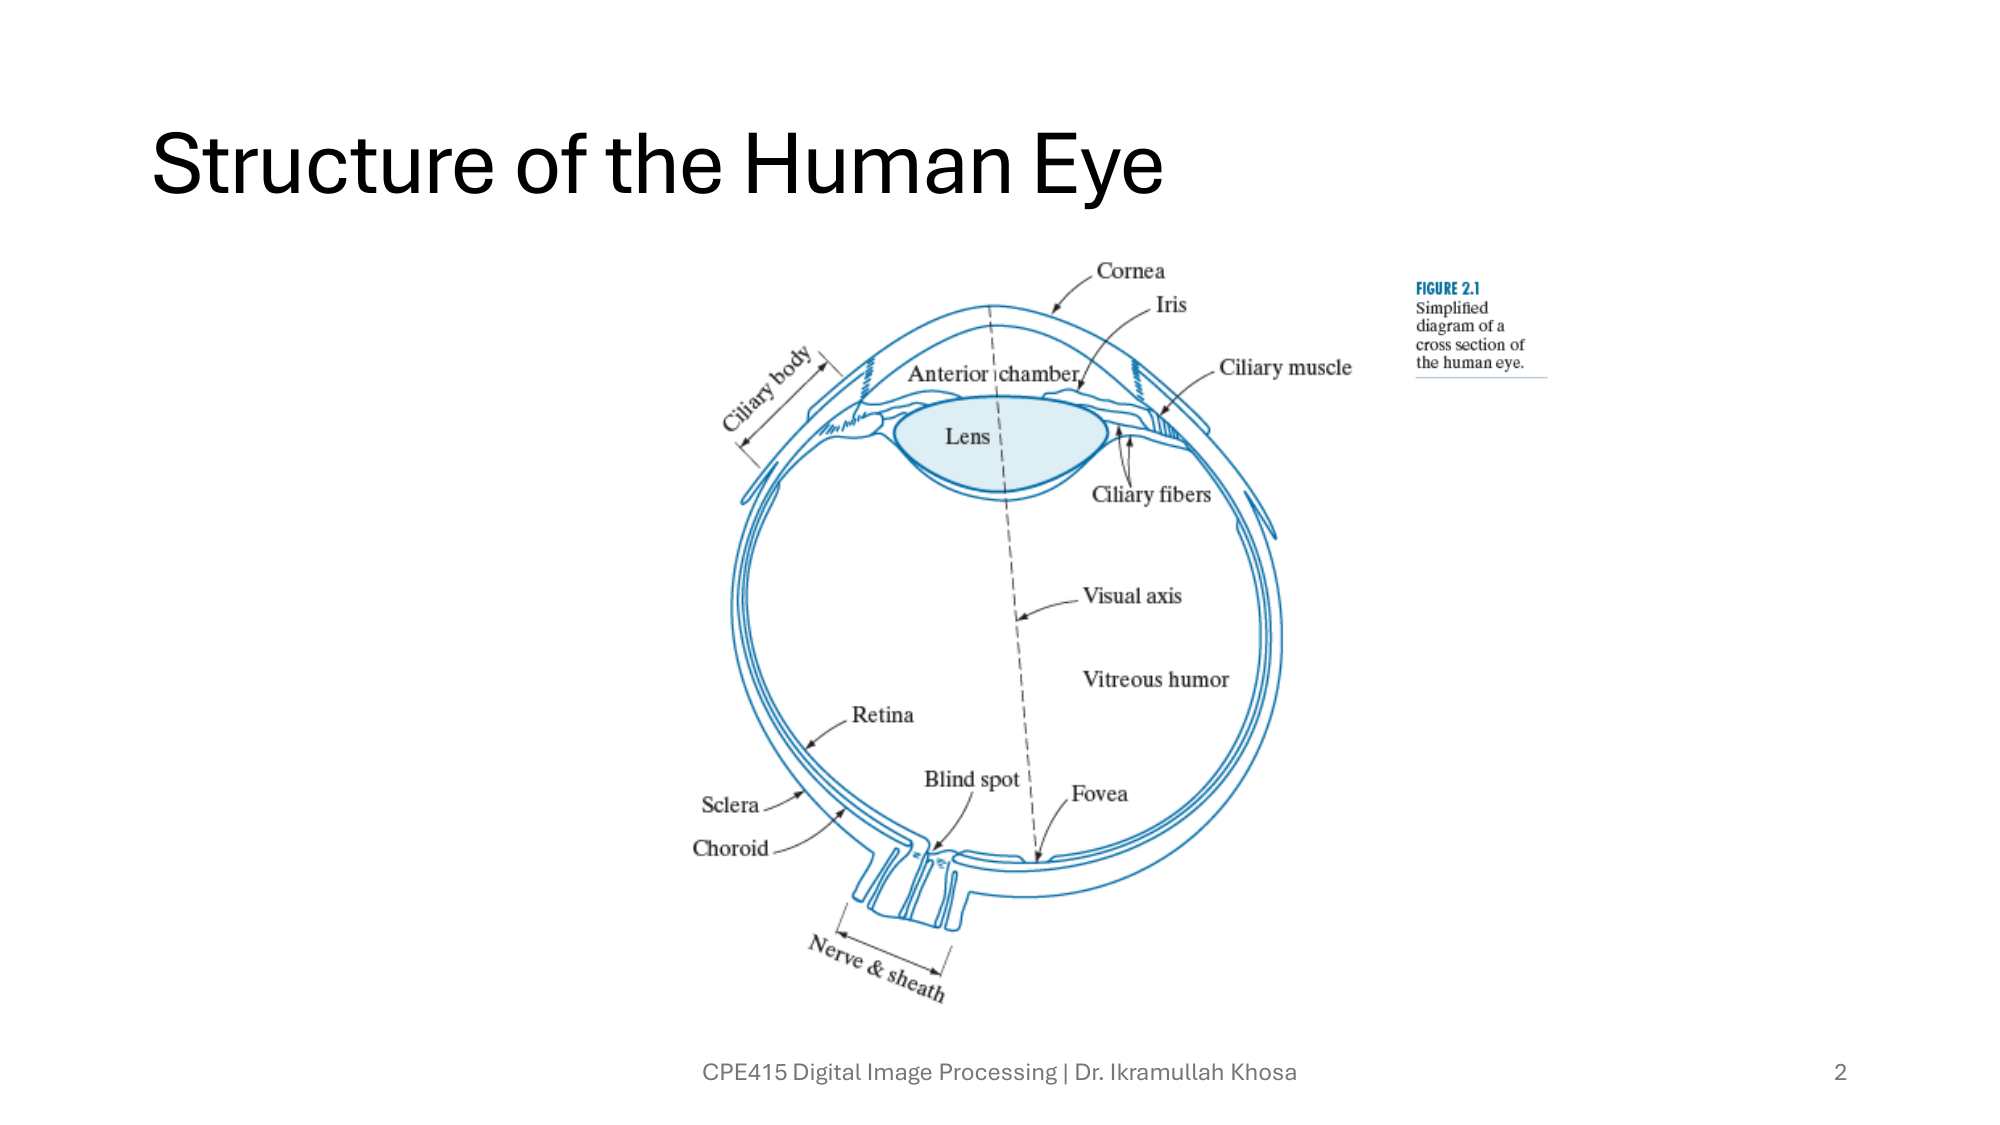
\includegraphics[width=0.85\textwidth]{images/slide2-02.png}
    \caption{Cross-section of the human eye showing major components}
    \label{fig:eye_structure}
\end{figure}

\begin{deepexplanation}
\textbf{DEEP ANALYSIS - Figure \ref{fig:eye_structure}: The Optical System of the Eye}

\textbf{Light Path Through the Eye:}
\begin{enumerate}
    \item \textbf{Cornea}: Transparent outer layer, provides \textbf{most of the focusing power} ($\approx 2/3$ of total). Fixed curvature means fixed focal length contribution.
    
    \item \textbf{Pupil \& Iris}: The pupil is the aperture (opening); the iris is the colored muscle that controls pupil size. Functions like a camera aperture:
    \begin{itemize}
        \item Bright light $\rightarrow$ small pupil (1.5--2 mm) $\rightarrow$ less light enters
        \item Dim light $\rightarrow$ large pupil (6--8 mm) $\rightarrow$ more light enters
        \item Range: $\approx$ 20:1 light intensity control
    \end{itemize}
    
    \item \textbf{Lens}: Flexible, provides \textbf{adjustable focus} (accommodation). Muscles change its shape:
    \begin{itemize}
        \item Relaxed: Flat lens $\rightarrow$ focuses distant objects
        \item Contracted: Rounded lens $\rightarrow$ focuses nearby objects
        \item This ability decreases with age (presbyopia)
    \end{itemize}
    
    \item \textbf{Vitreous Humor}: Gel-like substance filling the eye, maintains shape and transmits light.
    
    \item \textbf{Retina}: The ``sensor'' --- contains photoreceptor cells that convert light to neural signals.
\end{enumerate}

\textbf{Key Optical Properties:}
\begin{itemize}
    \item Total focal length: $\approx 17$ mm (when focused at infinity)
    \item Field of view: $\approx 180°$ horizontal, but high-resolution only in central $\approx 2°$
    \item Image is \textbf{inverted} on retina (brain corrects this)
\end{itemize}
\end{deepexplanation}

\begin{figure}[H]
    \centering
    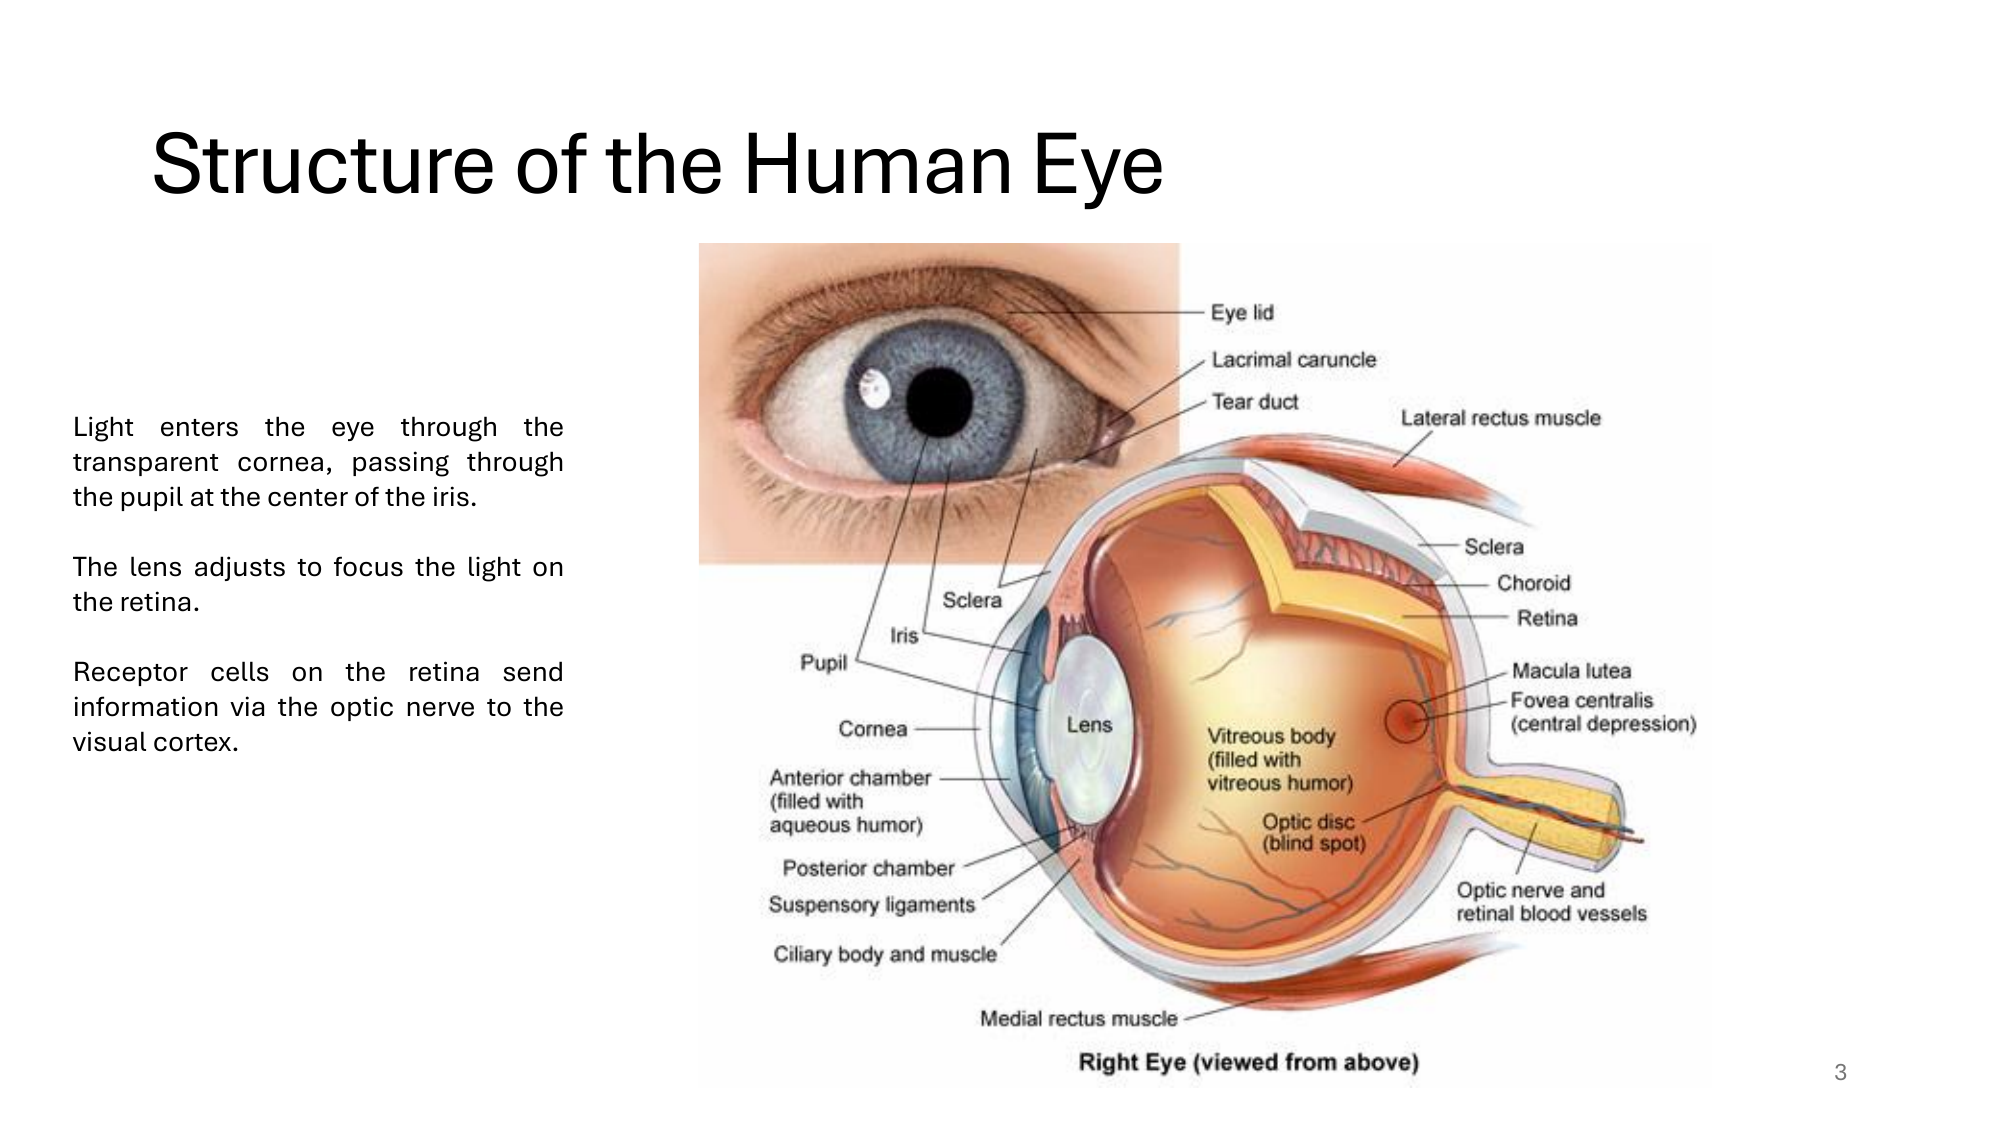
\includegraphics[width=0.85\textwidth]{images/slide2-03.png}
    \caption{Detailed view of eye structure}
    \label{fig:eye_detail}
\end{figure}

\begin{figure}[H]
    \centering
    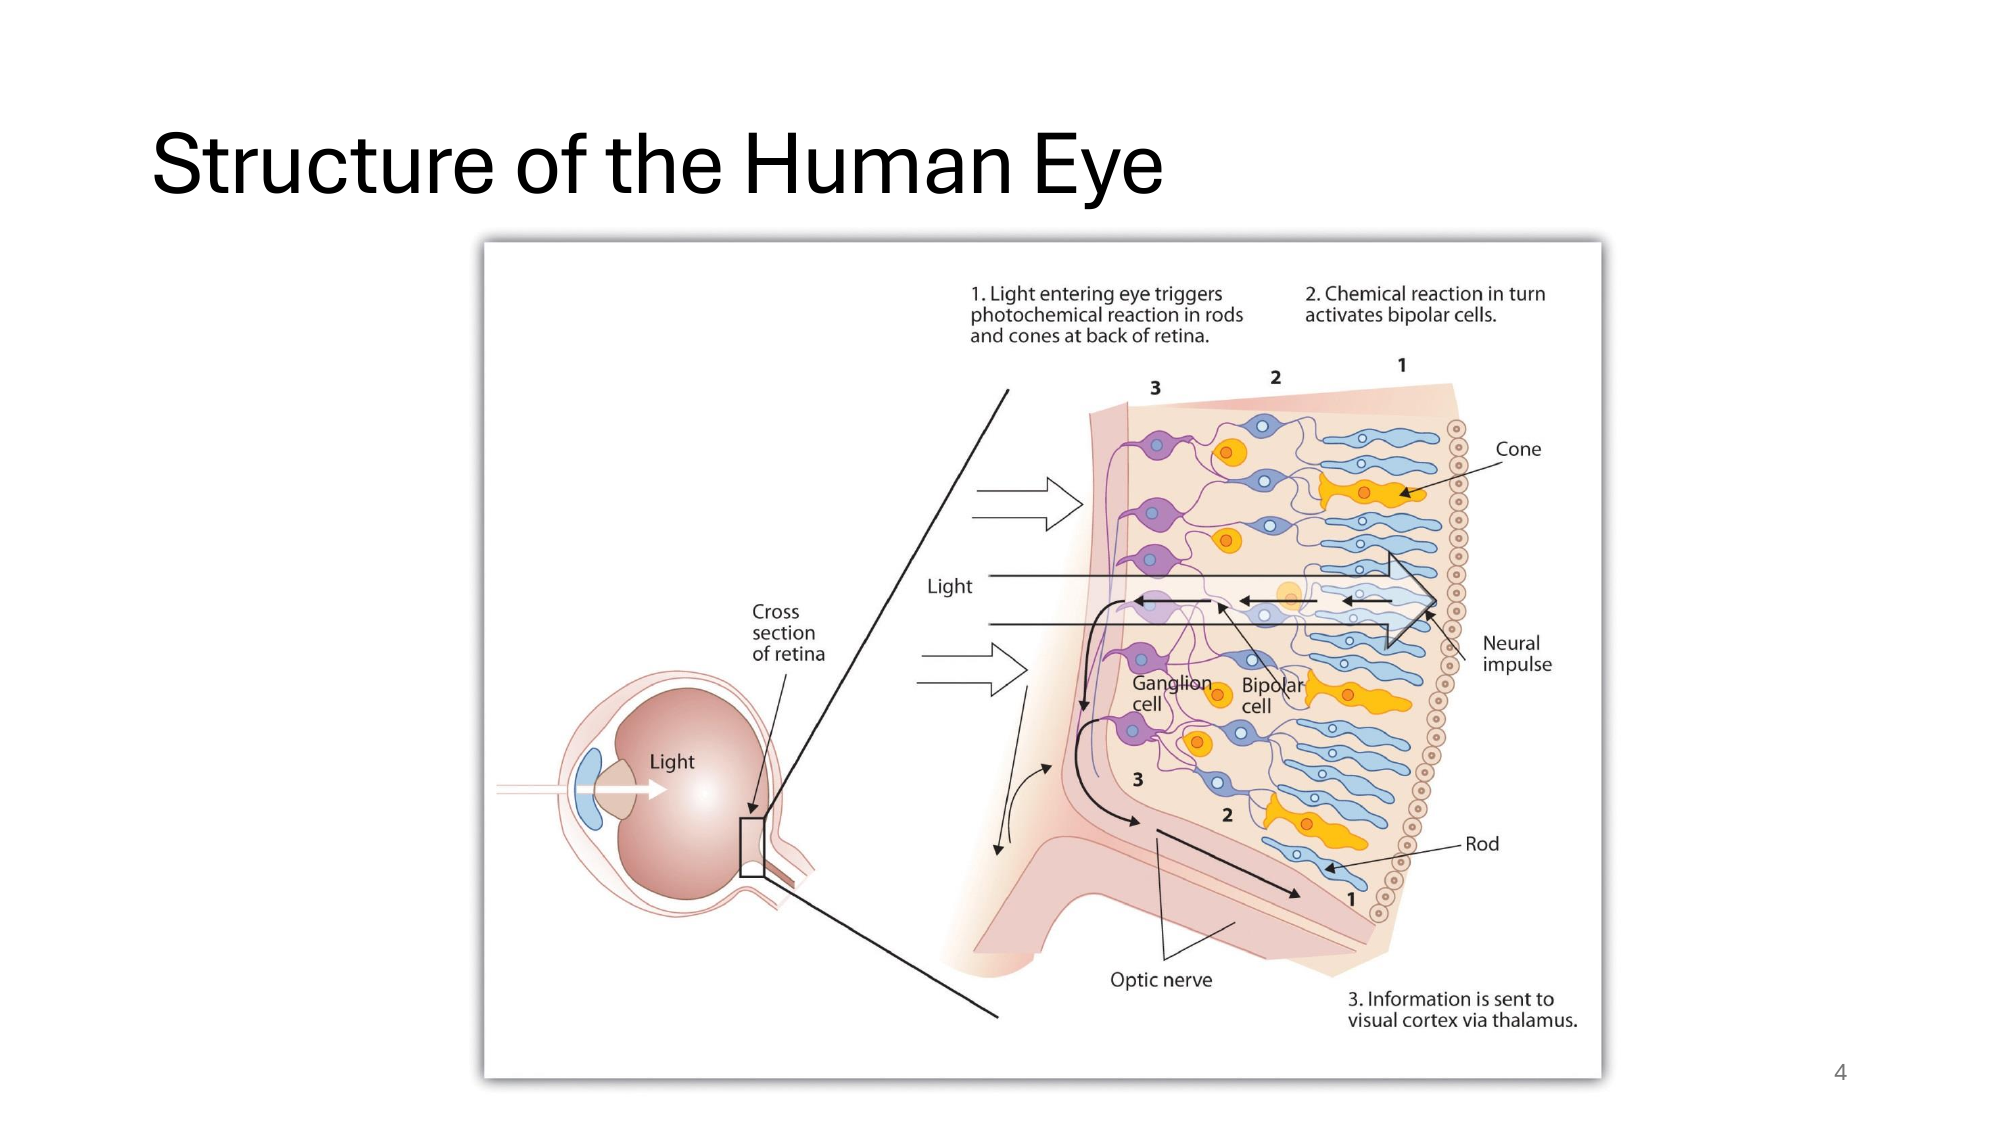
\includegraphics[width=0.9\textwidth]{images/slide2-04.png}
    \caption{Retinal photoreceptors: Cones and Rods}
    \label{fig:cones_rods}
\end{figure}

\begin{deepexplanation}
\textbf{DEEP ANALYSIS - Figure \ref{fig:cones_rods}: The Two Types of Photoreceptors}

\textbf{Cones (Color Vision):}
\begin{itemize}
    \item \textbf{Quantity}: 6--7 million per eye
    \item \textbf{Location}: Concentrated in the \textbf{fovea} (central retina)
    \item \textbf{Function}: Color vision and fine detail
    \item \textbf{Light sensitivity}: Require bright light (photopic vision)
    \item \textbf{Three types}: S (short/blue, $\approx 420$ nm), M (medium/green, $\approx 530$ nm), L (long/red, $\approx 560$ nm)
    \item \textbf{Acuity}: High --- responsible for sharp, detailed vision
\end{itemize}

\textbf{Rods (Low-Light Vision):}
\begin{itemize}
    \item \textbf{Quantity}: 75--150 million per eye (10-20× more than cones!)
    \item \textbf{Location}: Distributed across peripheral retina, \textbf{absent from fovea center}
    \item \textbf{Function}: Night vision and motion detection
    \item \textbf{Light sensitivity}: 1000× more sensitive than cones (scotopic vision)
    \item \textbf{Color}: \textbf{No color discrimination} --- only intensity (this is why colors are hard to see at night)
    \item \textbf{Acuity}: Low --- provides overall scene awareness, not detail
\end{itemize}

\textbf{Why Two Systems?}
Evolution optimized for both daylight (cones for color/detail) and night (rods for sensitivity). At twilight, both systems operate (mesopic vision).

\textbf{Implications for Image Processing:}
\begin{itemize}
    \item Color information is less important in peripheral vision
    \item Motion detection is highly sensitive (important for video compression)
    \item In dim images, color accuracy matters less than brightness
\end{itemize}
\end{deepexplanation}

\begin{figure}[H]
    \centering
    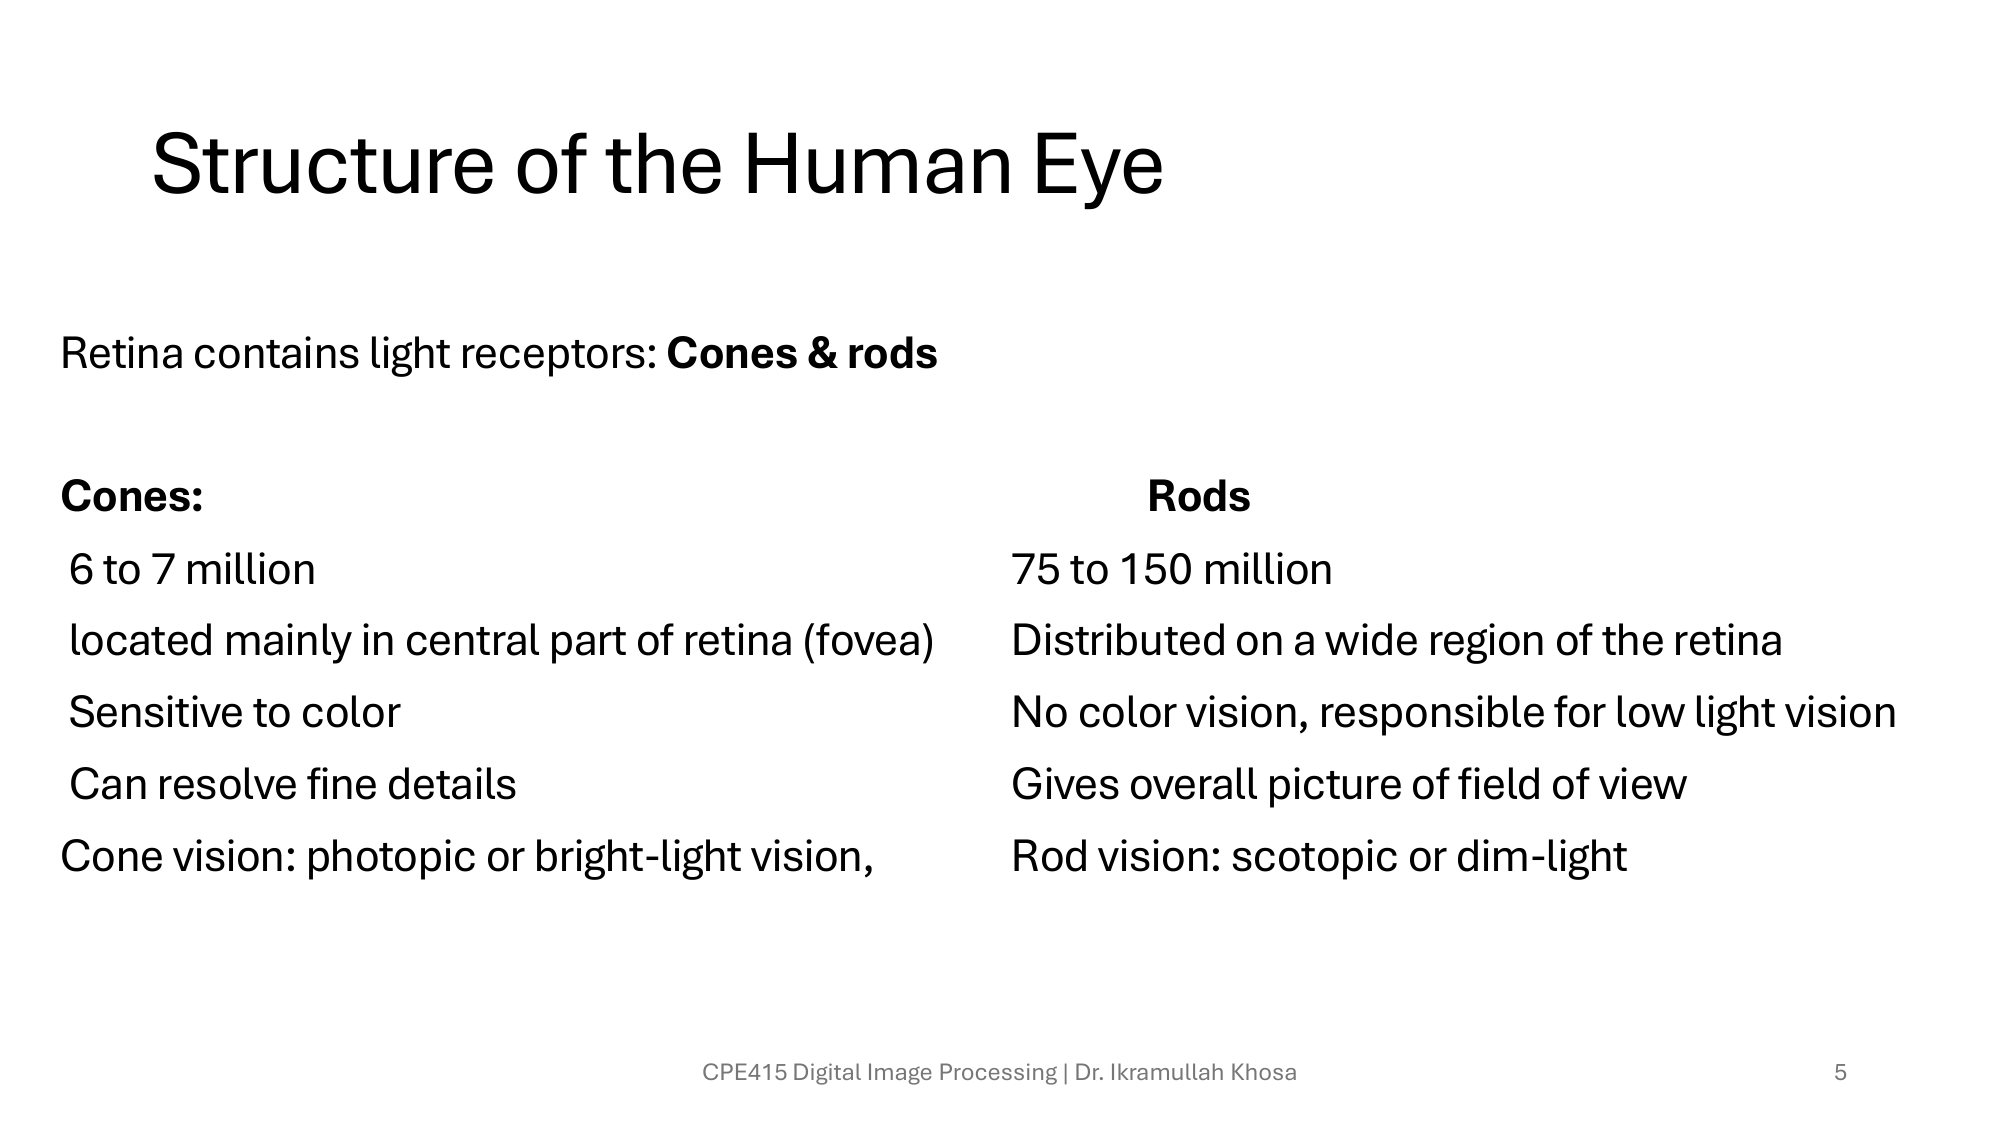
\includegraphics[width=0.85\textwidth]{images/slide2-05.png}
    \caption{Distribution of cones and rods across the retina}
    \label{fig:receptor_distribution}
\end{figure}

\begin{deepexplanation}
\textbf{DEEP ANALYSIS - Figure \ref{fig:receptor_distribution}: Spatial Distribution of Photoreceptors}

\textbf{What the Graph Shows:}
Density of cones and rods as a function of angular position from the fovea (center of vision).

\textbf{Key Observations:}

\textbf{1. The Fovea (0° position):}
\begin{itemize}
    \item Extremely high cone density: $\approx 150,000$ cones/mm²
    \item Zero or very few rods
    \item Diameter: $\approx 1.5$ mm ($\approx 1.77$ mm²)
    \item Total cones in fovea: $\approx 265,000$
    \item This is where you see fine detail (reading this text uses your fovea)
\end{itemize}

\textbf{2. The Blind Spot ($\approx 15°$ from fovea):}
\begin{itemize}
    \item Zero receptors of either type
    \item Location where optic nerve exits the eye
    \item Brain ``fills in'' this gap --- you don't perceive it
\end{itemize}

\textbf{3. Peripheral Retina:}
\begin{itemize}
    \item Dominated by rods
    \item Cone density drops rapidly away from fovea
    \item Rod density peaks at $\approx 20°$ from fovea
\end{itemize}

\textbf{Practical Implications:}
\begin{itemize}
    \item To see something clearly, you must look directly at it (foveate)
    \item Peripheral vision is good for motion, not detail
    \item Foveated rendering in VR: high resolution only where user looks
\end{itemize}

\textbf{Comparison with Digital Sensors:}
\begin{itemize}
    \item Fovea: $\approx 265,000$ ``pixels'' in 1.77 mm² = 150,000 pixels/mm²
    \item Modern cameras: Can exceed this density, but uniform across entire sensor
    \item Eye is spatially-variant; cameras are typically spatially-invariant
\end{itemize}
\end{deepexplanation}

\begin{figure}[H]
    \centering
    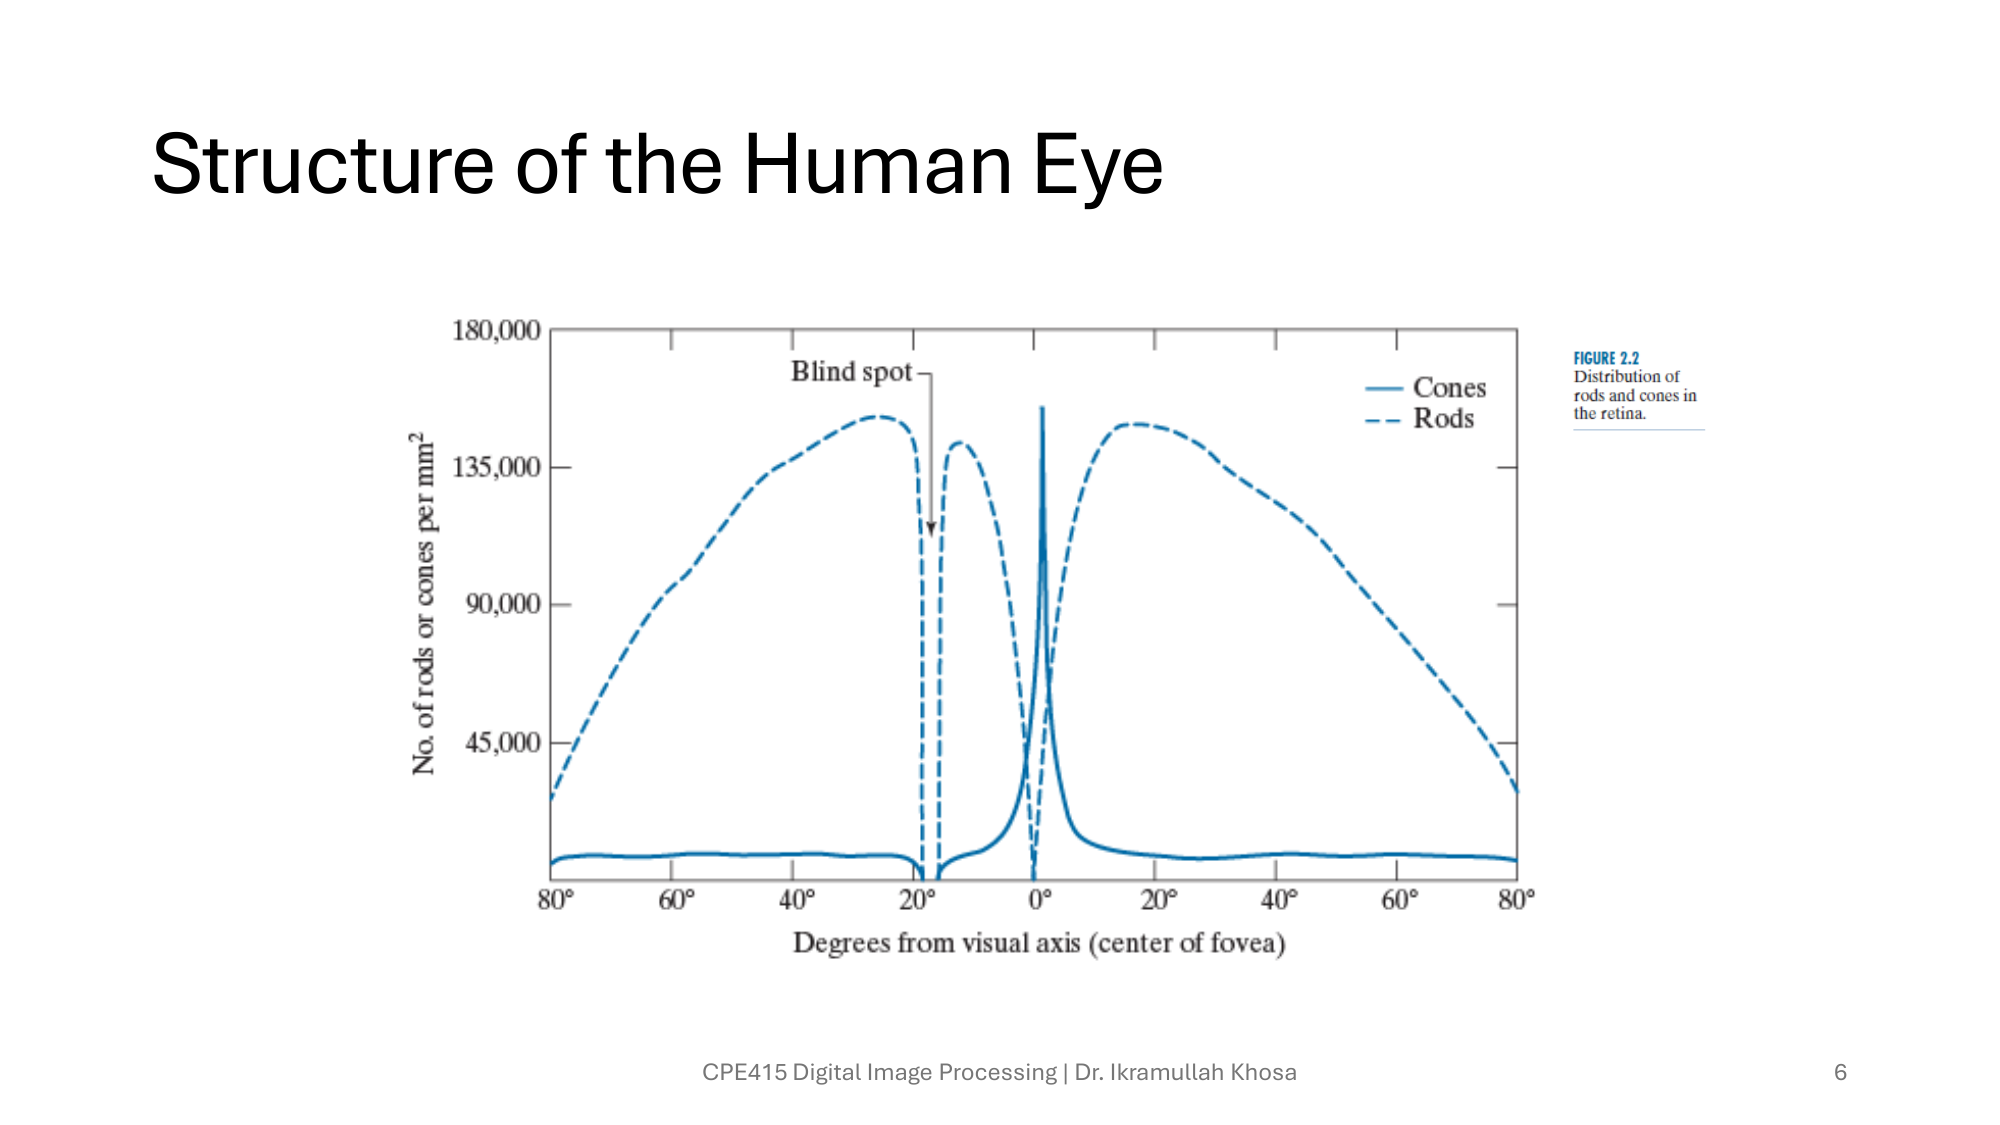
\includegraphics[width=0.8\textwidth]{images/slide2-06.png}
    \caption{Fovea structure and receptor density}
    \label{fig:fovea_detail}
\end{figure}

\subsection{Image Formation in the Eye}

\begin{figure}[H]
    \centering
    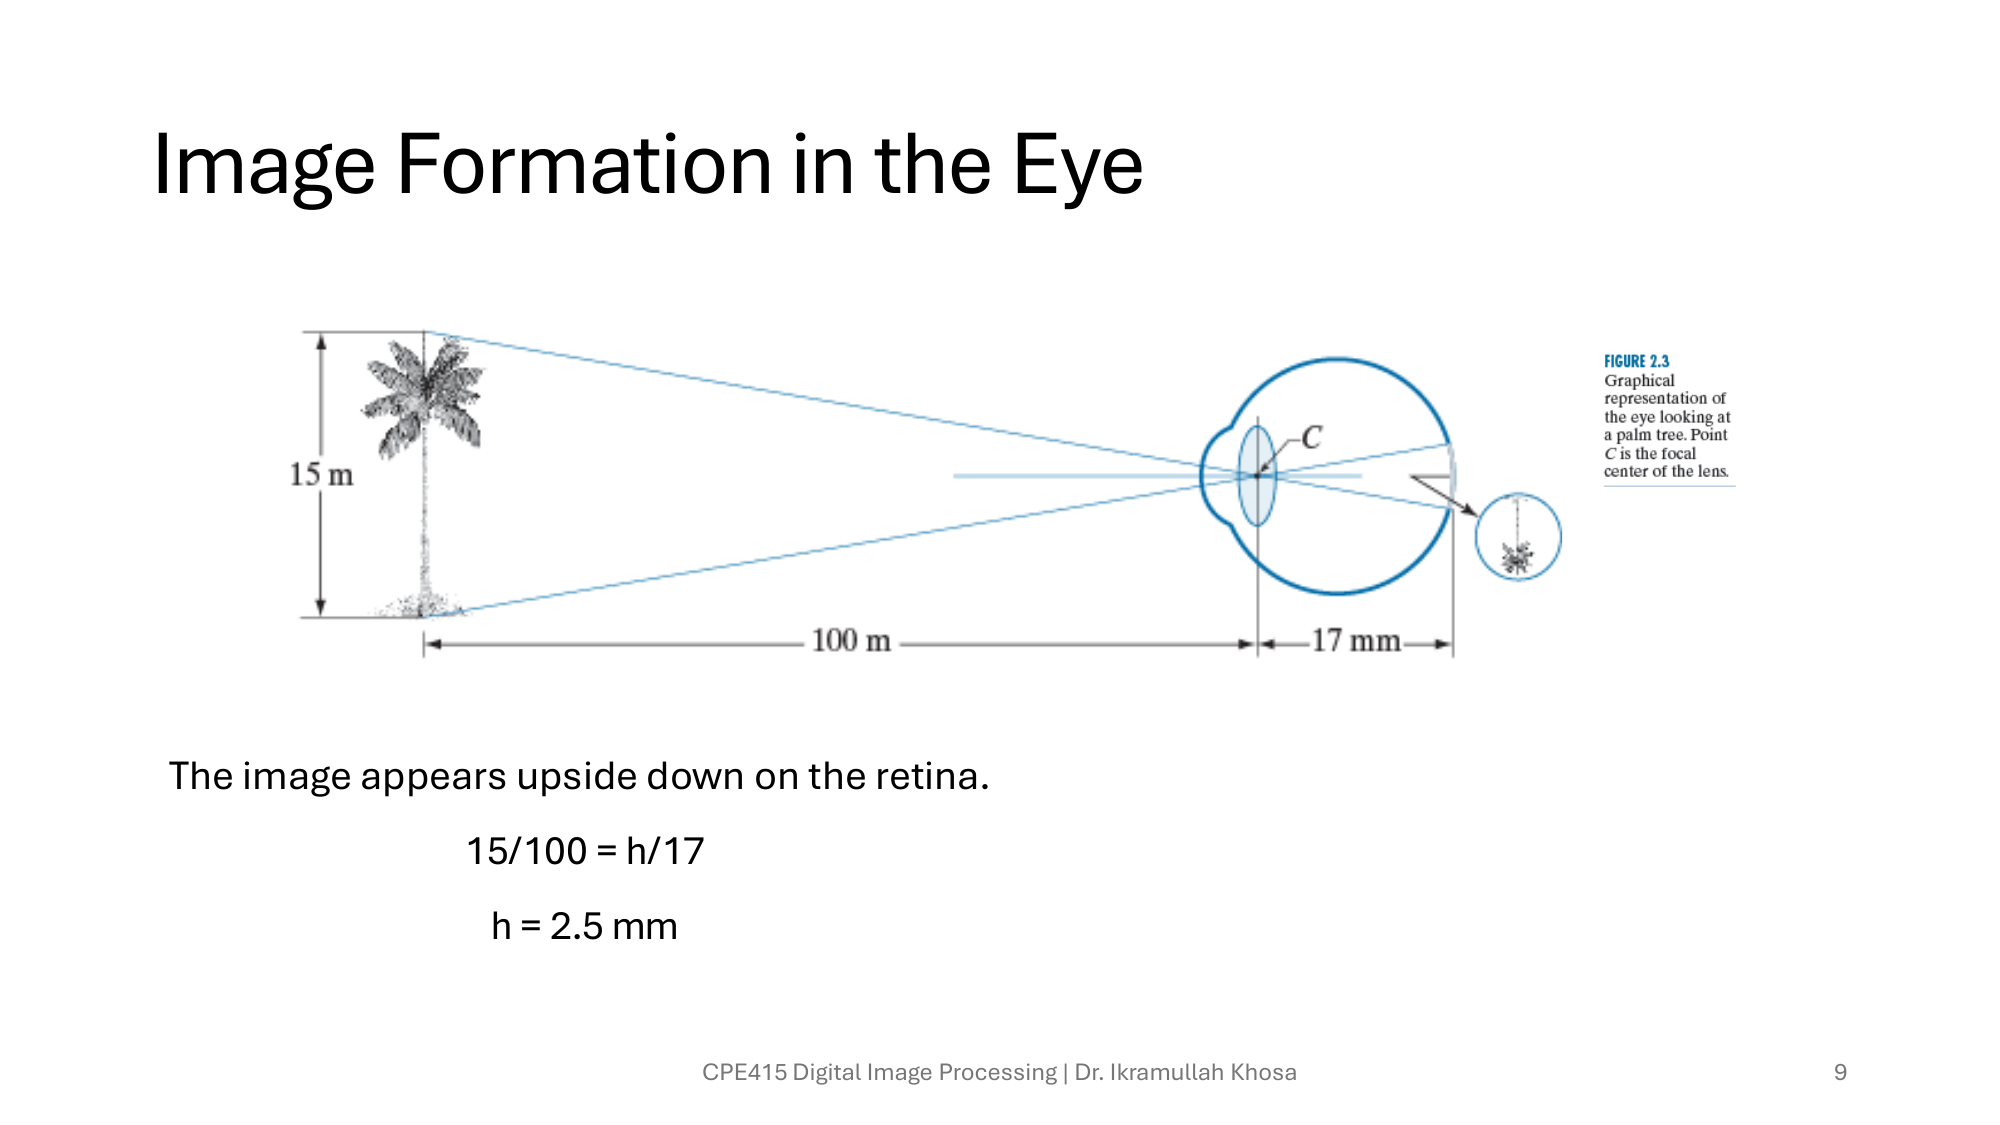
\includegraphics[width=0.85\textwidth]{images/slide2-09.png}
    \caption{Image formation on the retina}
    \label{fig:image_formation}
\end{figure}

\begin{deepexplanation}
\textbf{DEEP ANALYSIS - Figure \ref{fig:image_formation}: The Optics of Vision}

\textbf{The Thin Lens Equation:}
\[
\frac{1}{d_o} + \frac{1}{d_i} = \frac{1}{f}
\]
where $d_o$ = object distance, $d_i$ = image distance, $f$ = focal length.

For the eye: $d_i \approx 17$ mm (fixed), so the lens adjusts $f$ via accommodation.

\textbf{Image Size Calculation (from the figure):}
Given:
\begin{itemize}
    \item Object height: 15 cm
    \item Object distance: 100 cm (1 meter)
    \item Eye depth: 17 mm
\end{itemize}

Using similar triangles:
\[
\frac{\text{image height}}{\text{retinal distance}} = \frac{\text{object height}}{\text{object distance}}
\]
\[
\frac{h}{17 \text{ mm}} = \frac{15 \text{ cm}}{100 \text{ cm}} \implies h = 17 \times 0.15 = 2.55 \text{ mm}
\]

\textbf{Key Points:}
\begin{itemize}
    \item Image is \textbf{inverted} (upside down) on the retina
    \item Image is \textbf{real} (light actually focuses there, unlike virtual images)
    \item Brain interprets the inverted image correctly (learned from birth)
\end{itemize}

\textbf{Why This Matters:}
\begin{itemize}
    \item Camera sensors are designed similarly (real, inverted images)
    \item Optical aberrations in the eye affect image quality
    \item Understanding eye optics helps design better displays and imaging systems
\end{itemize}
\end{deepexplanation}

\subsection{Brightness Adaptation and Discrimination}

\begin{figure}[H]
    \centering
    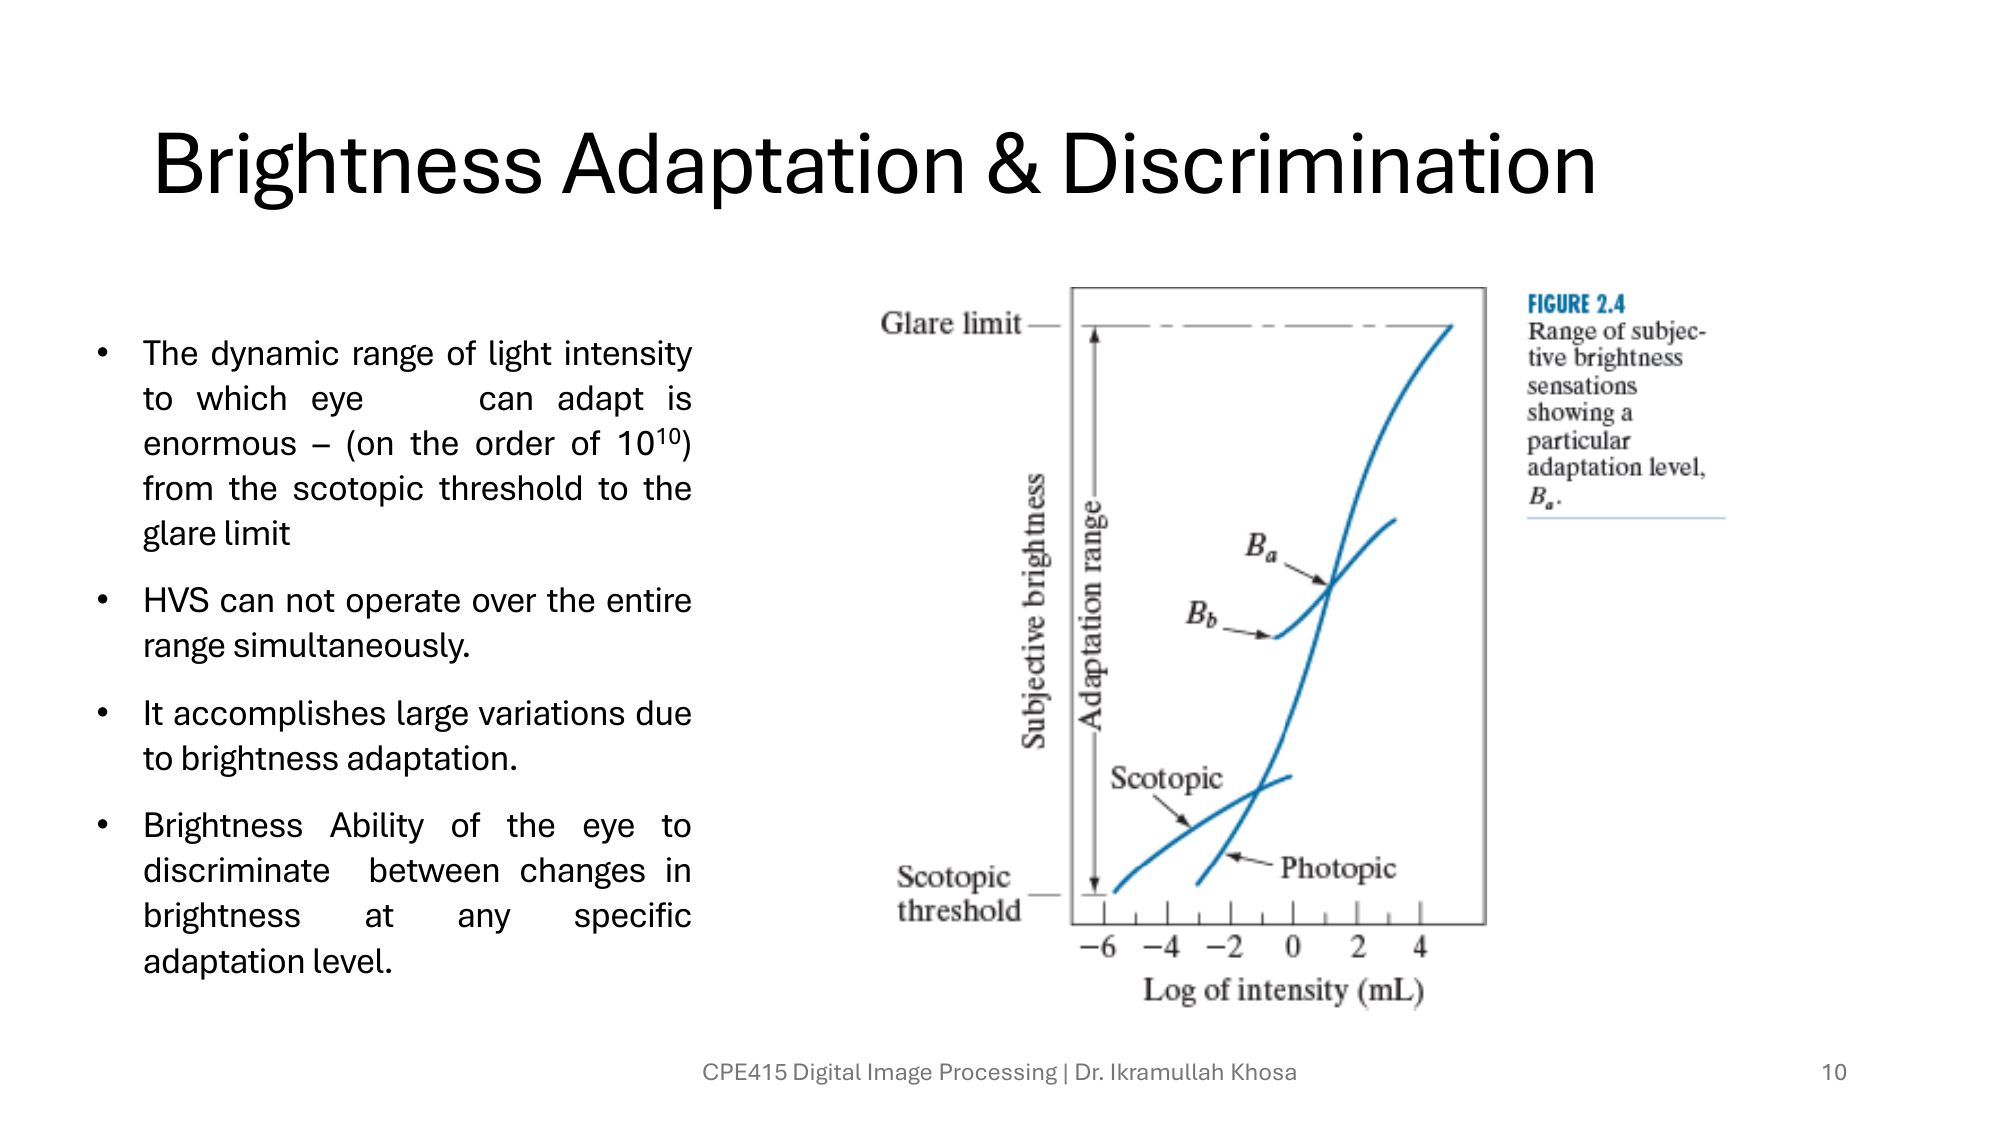
\includegraphics[width=0.9\textwidth]{images/slide2-10.png}
    \caption{Human visual system brightness adaptation range}
    \label{fig:brightness_adaptation}
\end{figure}

\begin{deepexplanation}
\textbf{DEEP ANALYSIS - Figure \ref{fig:brightness_adaptation}: The Enormous Dynamic Range of Vision}

\textbf{The Adaptation Range:}
The human visual system can respond to light intensities spanning \textbf{10 orders of magnitude} ($10^{10}$):
\begin{itemize}
    \item \textbf{Scotopic threshold}: $\approx 10^{-6}$ cd/m² (starlight, dark-adapted)
    \item \textbf{Glare limit}: $\approx 10^{4}$ cd/m² (painful brightness)
    \item Total range: $10^{4} / 10^{-6} = 10^{10}$
\end{itemize}

\textbf{But NOT Simultaneously!}
\begin{itemize}
    \item At any moment, the eye operates over only $\approx 2$--$3$ orders of magnitude
    \item The operating range \textbf{shifts} via brightness adaptation
    \item Adaptation takes time: Light-to-dark $\approx 30$ minutes; dark-to-light $\approx 5$ minutes
\end{itemize}

\textbf{How Adaptation Works:}
\begin{enumerate}
    \item \textbf{Pupil size}: Fast (seconds), limited range ($\approx 20:1$)
    \item \textbf{Photochemical}: Regeneration of photopigments (minutes)
    \item \textbf{Neural}: Gain control in retinal circuits
\end{enumerate}

\textbf{Implications for Image Processing:}
\begin{itemize}
    \item HDR imaging captures more than eye can see at once
    \item Tone mapping compresses HDR to displayable range
    \item Display brightness must match viewing conditions
    \item 8-bit images ($256$ levels) are sufficient for most displays because eye can only discriminate $\approx 100$--$200$ levels at any adaptation
\end{itemize}
\end{deepexplanation}

\begin{figure}[H]
    \centering
    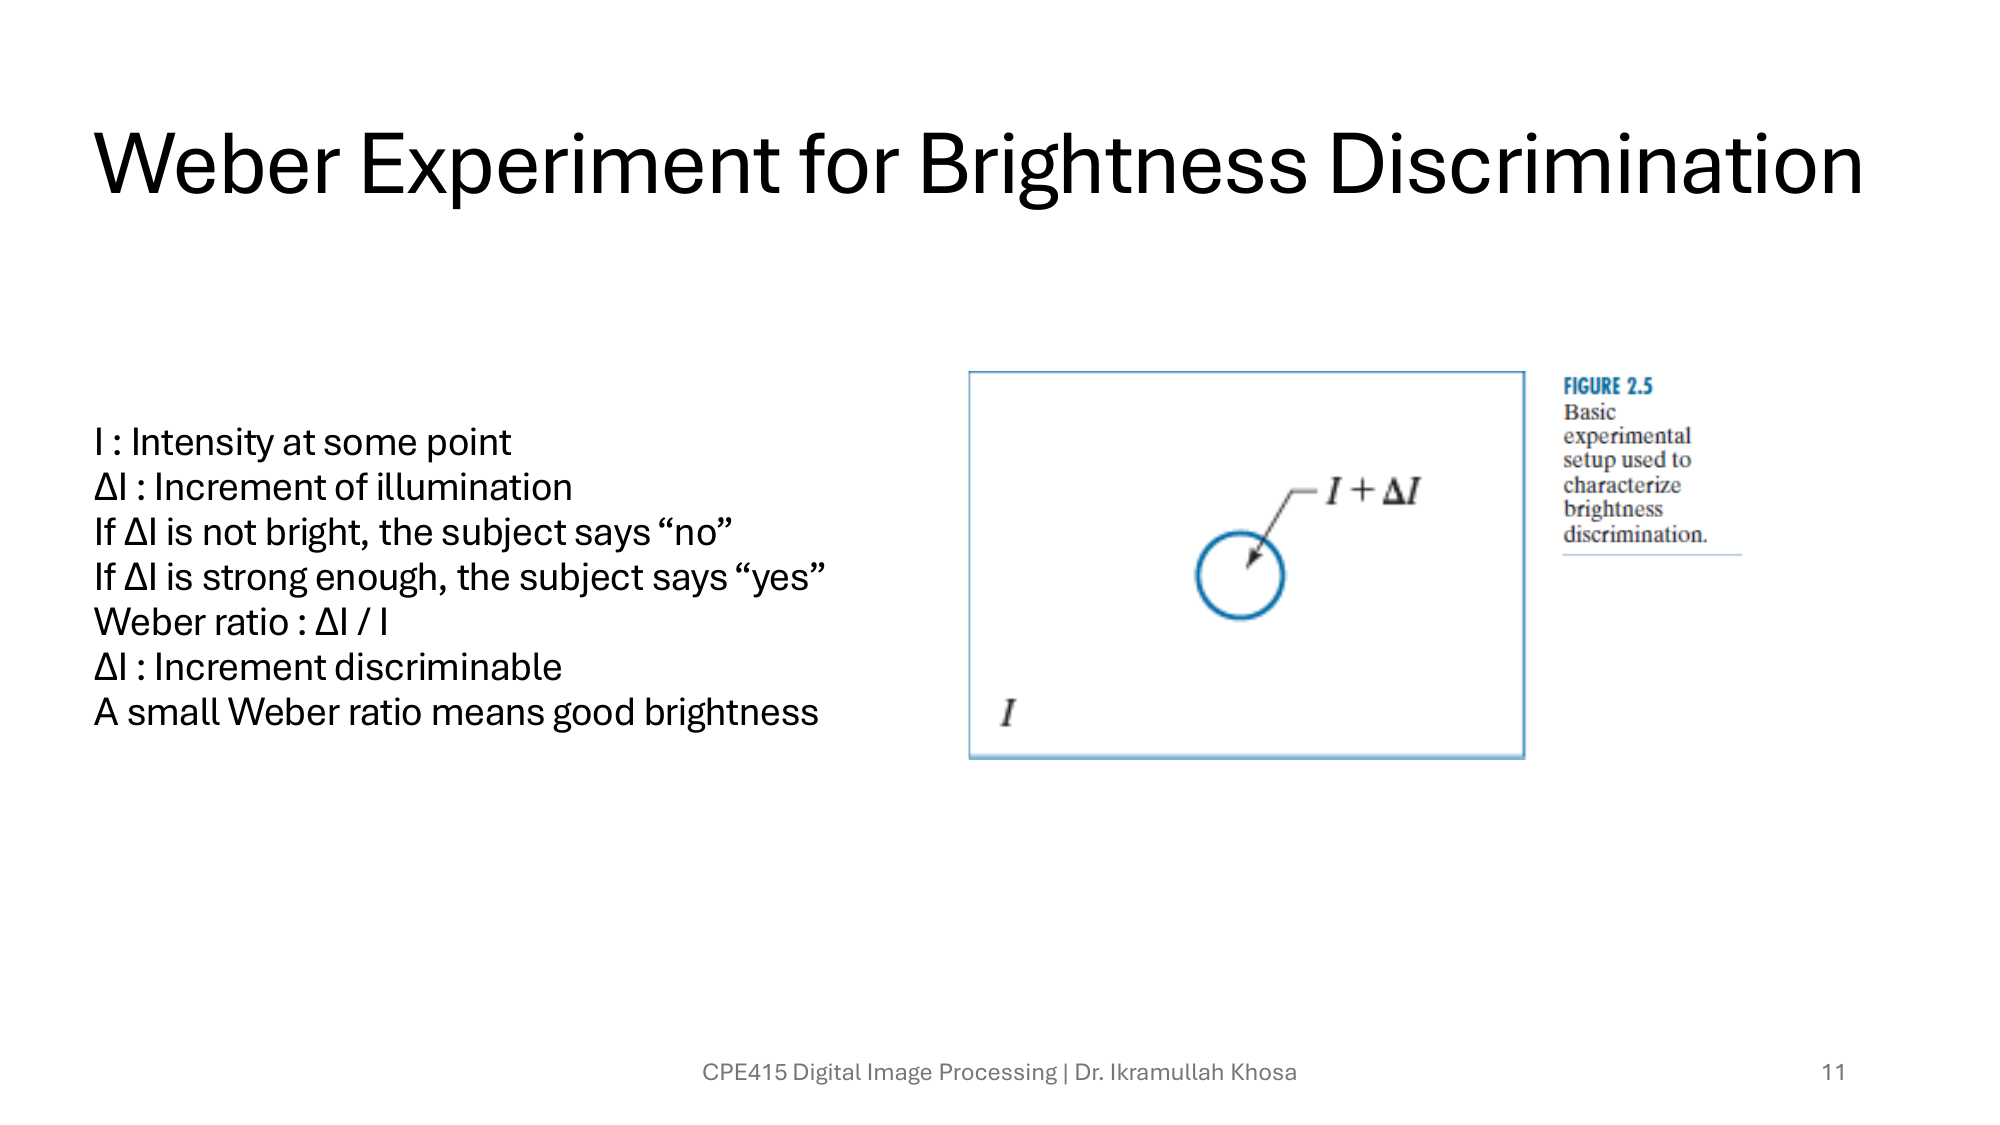
\includegraphics[width=0.85\textwidth]{images/slide2-11.png}
    \caption{Weber's experiment for brightness discrimination}
    \label{fig:weber_experiment}
\end{figure}

\begin{deepexplanation}
\textbf{DEEP ANALYSIS - Figure \ref{fig:weber_experiment}: Weber's Law and JND}

\textbf{The Experiment:}
\begin{enumerate}
    \item Subject views a uniform field at intensity $I$
    \item A small test spot with intensity $I + \Delta I$ is briefly shown
    \item Subject reports whether they can see the difference
    \item The minimum $\Delta I$ detectable is measured
\end{enumerate}

\textbf{Weber's Law:}
\[
\frac{\Delta I}{I} = k \approx 0.01 \text{ to } 0.02 \text{ (constant)}
\]

\textbf{What This Means:}
\begin{itemize}
    \item The \textbf{Just Noticeable Difference (JND)} is proportional to background intensity
    \item At $I = 100$, need $\Delta I \approx 1$--$2$ to notice a difference
    \item At $I = 1000$, need $\Delta I \approx 10$--$20$
    \item \textbf{Relative} change matters, not \textbf{absolute} change
\end{itemize}

\textbf{The Weber Ratio:}
A small Weber ratio = good brightness discrimination:
\[
\text{Weber ratio} = \frac{\Delta I_c}{I}
\]
where $\Delta I_c$ is the minimum discriminable increment.

\textbf{Practical Implications:}
\begin{itemize}
    \item \textbf{Logarithmic quantization}: Since perception is relative, using log-spaced intensity levels is efficient
    \item \textbf{Gamma encoding}: Allocates more bits to dark regions (where Weber ratio would otherwise waste precision)
    \item \textbf{Why 8 bits work}: $256$ levels with gamma encoding spans perceptual range adequately
\end{itemize}
\end{deepexplanation}

\begin{figure}[H]
    \centering
    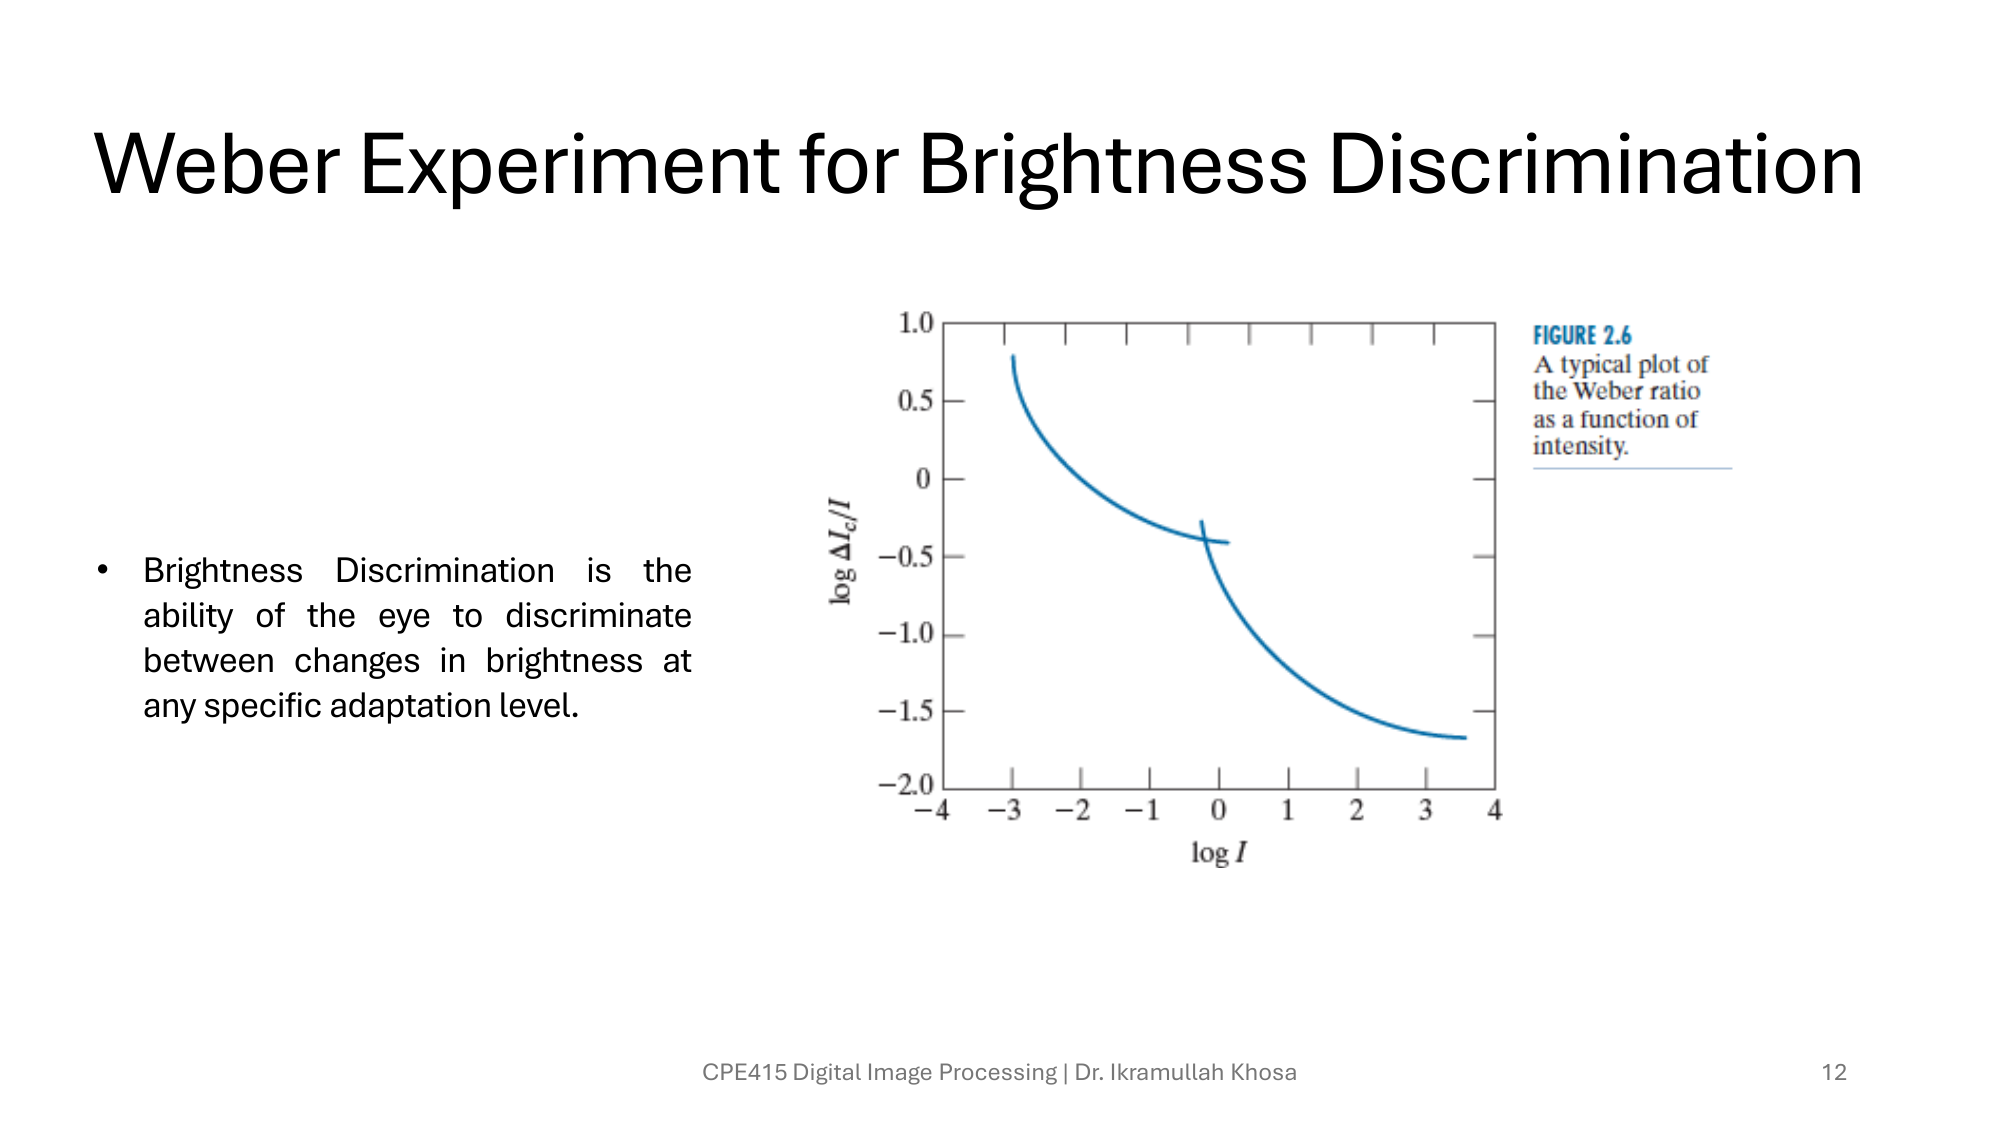
\includegraphics[width=0.85\textwidth]{images/slide2-12.png}
    \caption{Weber ratio as a function of intensity}
    \label{fig:weber_ratio}
\end{figure}

\subsection{Visual Phenomena: Mach Bands and Contrast}

\begin{figure}[H]
    \centering
    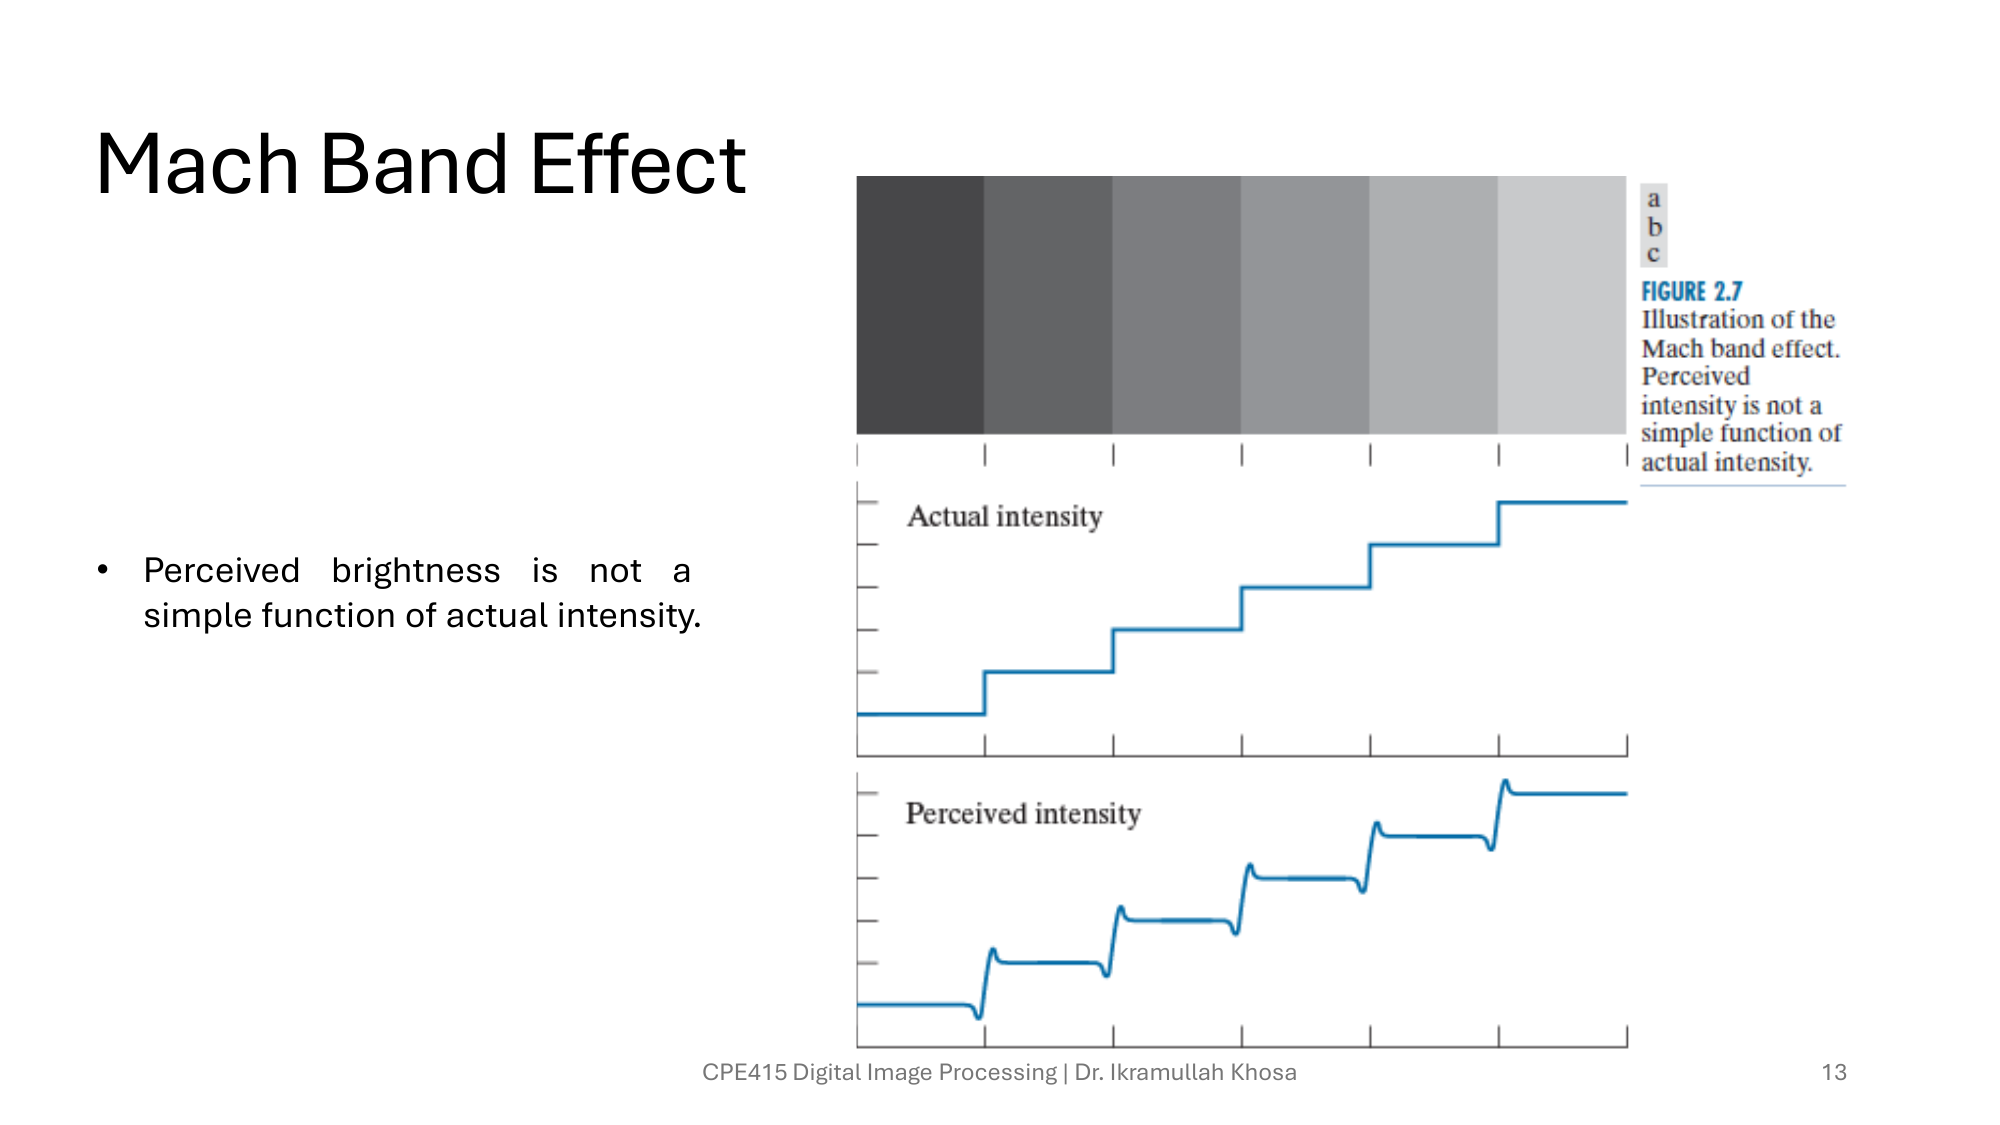
\includegraphics[width=0.85\textwidth]{images/slide2-13.png}
    \caption{Mach band effect demonstration}
    \label{fig:mach_bands}
\end{figure}

\begin{deepexplanation}
\textbf{DEEP ANALYSIS - Figure \ref{fig:mach_bands}: The Mach Band Illusion}

\textbf{What You See:}
At boundaries between regions of different intensity, you perceive:
\begin{itemize}
    \item A \textbf{bright band} on the lighter side of the edge
    \item A \textbf{dark band} on the darker side of the edge
\end{itemize}
These bands don't exist in the actual intensity profile!

\textbf{The Actual vs. Perceived Intensity:}
\begin{itemize}
    \item Actual: Step or ramp transition between two constant levels
    \item Perceived: Overshoot (bright band) and undershoot (dark band) at edges
\end{itemize}

\textbf{Why This Happens --- Lateral Inhibition:}
\begin{enumerate}
    \item Retinal ganglion cells have center-surround receptive fields
    \item Each cell is excited by light in its center, inhibited by light in its surround
    \item At an edge:
    \begin{itemize}
        \item Cells on bright side: Neighbors on dark side don't inhibit much $\rightarrow$ cell fires more $\rightarrow$ appears brighter
        \item Cells on dark side: Neighbors on bright side inhibit strongly $\rightarrow$ cell fires less $\rightarrow$ appears darker
    \end{itemize}
\end{enumerate}

\textbf{Why This Matters for Image Processing:}
\begin{itemize}
    \item \textbf{Edge enhancement}: Natural visual system already sharpens edges
    \item \textbf{Unsharp masking}: Mimics this effect artificially
    \item \textbf{Quantization}: Mach bands can appear at boundaries between quantization levels (contouring artifact)
    \item \textbf{Display calibration}: Must account for perceptual effects
\end{itemize}
\end{deepexplanation}

\begin{figure}[H]
    \centering
    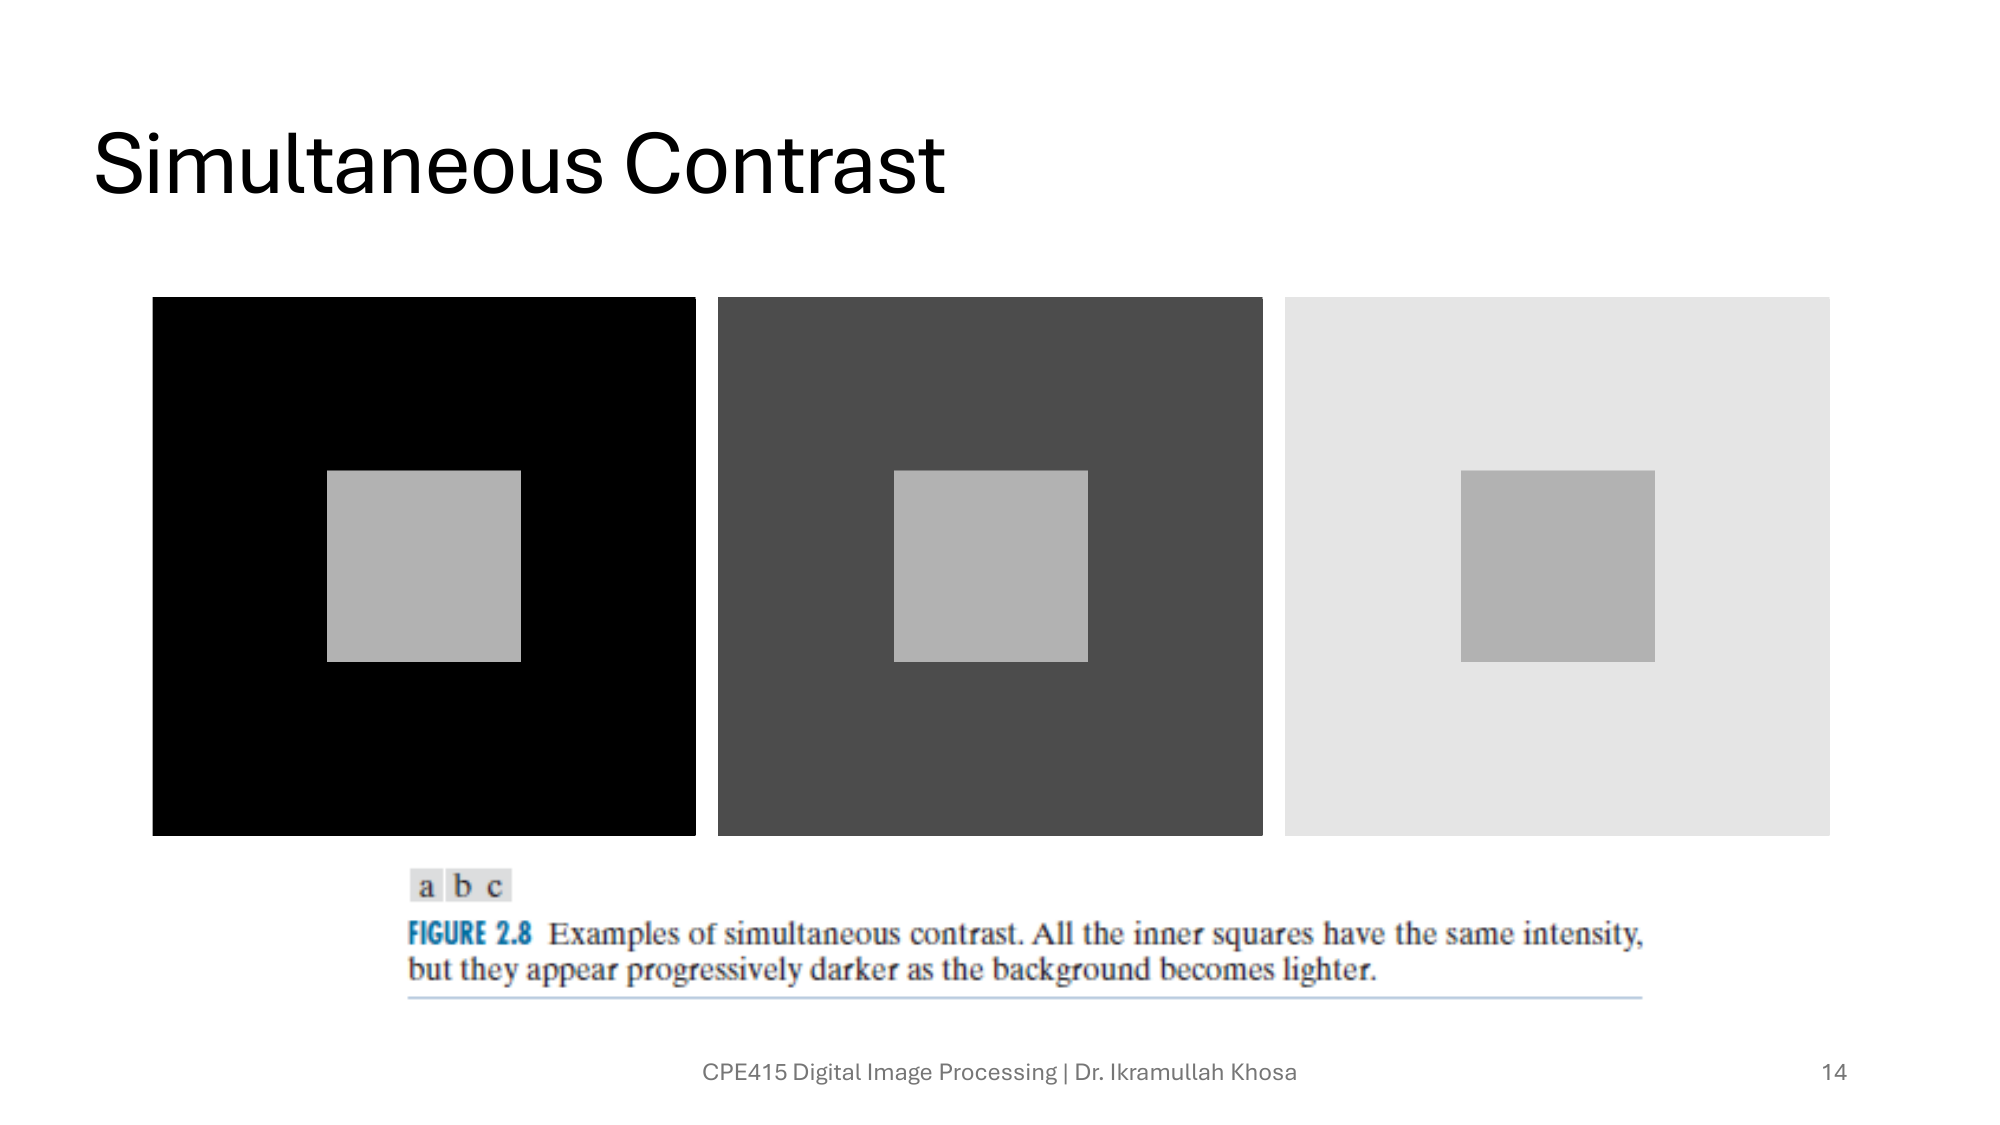
\includegraphics[width=0.85\textwidth]{images/slide2-14.png}
    \caption{Simultaneous contrast illusion}
    \label{fig:simultaneous_contrast}
\end{figure}

\begin{deepexplanation}
\textbf{DEEP ANALYSIS - Figure \ref{fig:simultaneous_contrast}: Context Affects Perception}

\textbf{The Illusion:}
Two squares of \textbf{identical gray level} appear different when placed on different backgrounds:
\begin{itemize}
    \item On a dark background: The gray square appears \textbf{lighter}
    \item On a light background: The same gray square appears \textbf{darker}
\end{itemize}

\textbf{The Neural Mechanism:}
Again, lateral inhibition is responsible:
\begin{itemize}
    \item Cells viewing the gray square on dark background: Little inhibition from dark surround $\rightarrow$ higher response $\rightarrow$ appears lighter
    \item Cells viewing the gray square on light background: Strong inhibition from bright surround $\rightarrow$ lower response $\rightarrow$ appears darker
\end{itemize}

\textbf{Why This Matters:}
\begin{itemize}
    \item \textbf{Color constancy}: Real-world perception compensates for illumination changes
    \item \textbf{Image display}: The same image looks different on different backgrounds (important for GUI design)
    \item \textbf{Histogram equalization}: Improves local contrast, compensating for simultaneous contrast limitations
    \item \textbf{Relative measurements}: In image analysis, \textbf{relative} rather than \textbf{absolute} intensity often matters
\end{itemize}

\textbf{Practical Demonstration:}
Cover the boundary between the two backgrounds with your finger --- the two gray squares will suddenly appear identical!
\end{deepexplanation}

\begin{figure}[H]
    \centering
    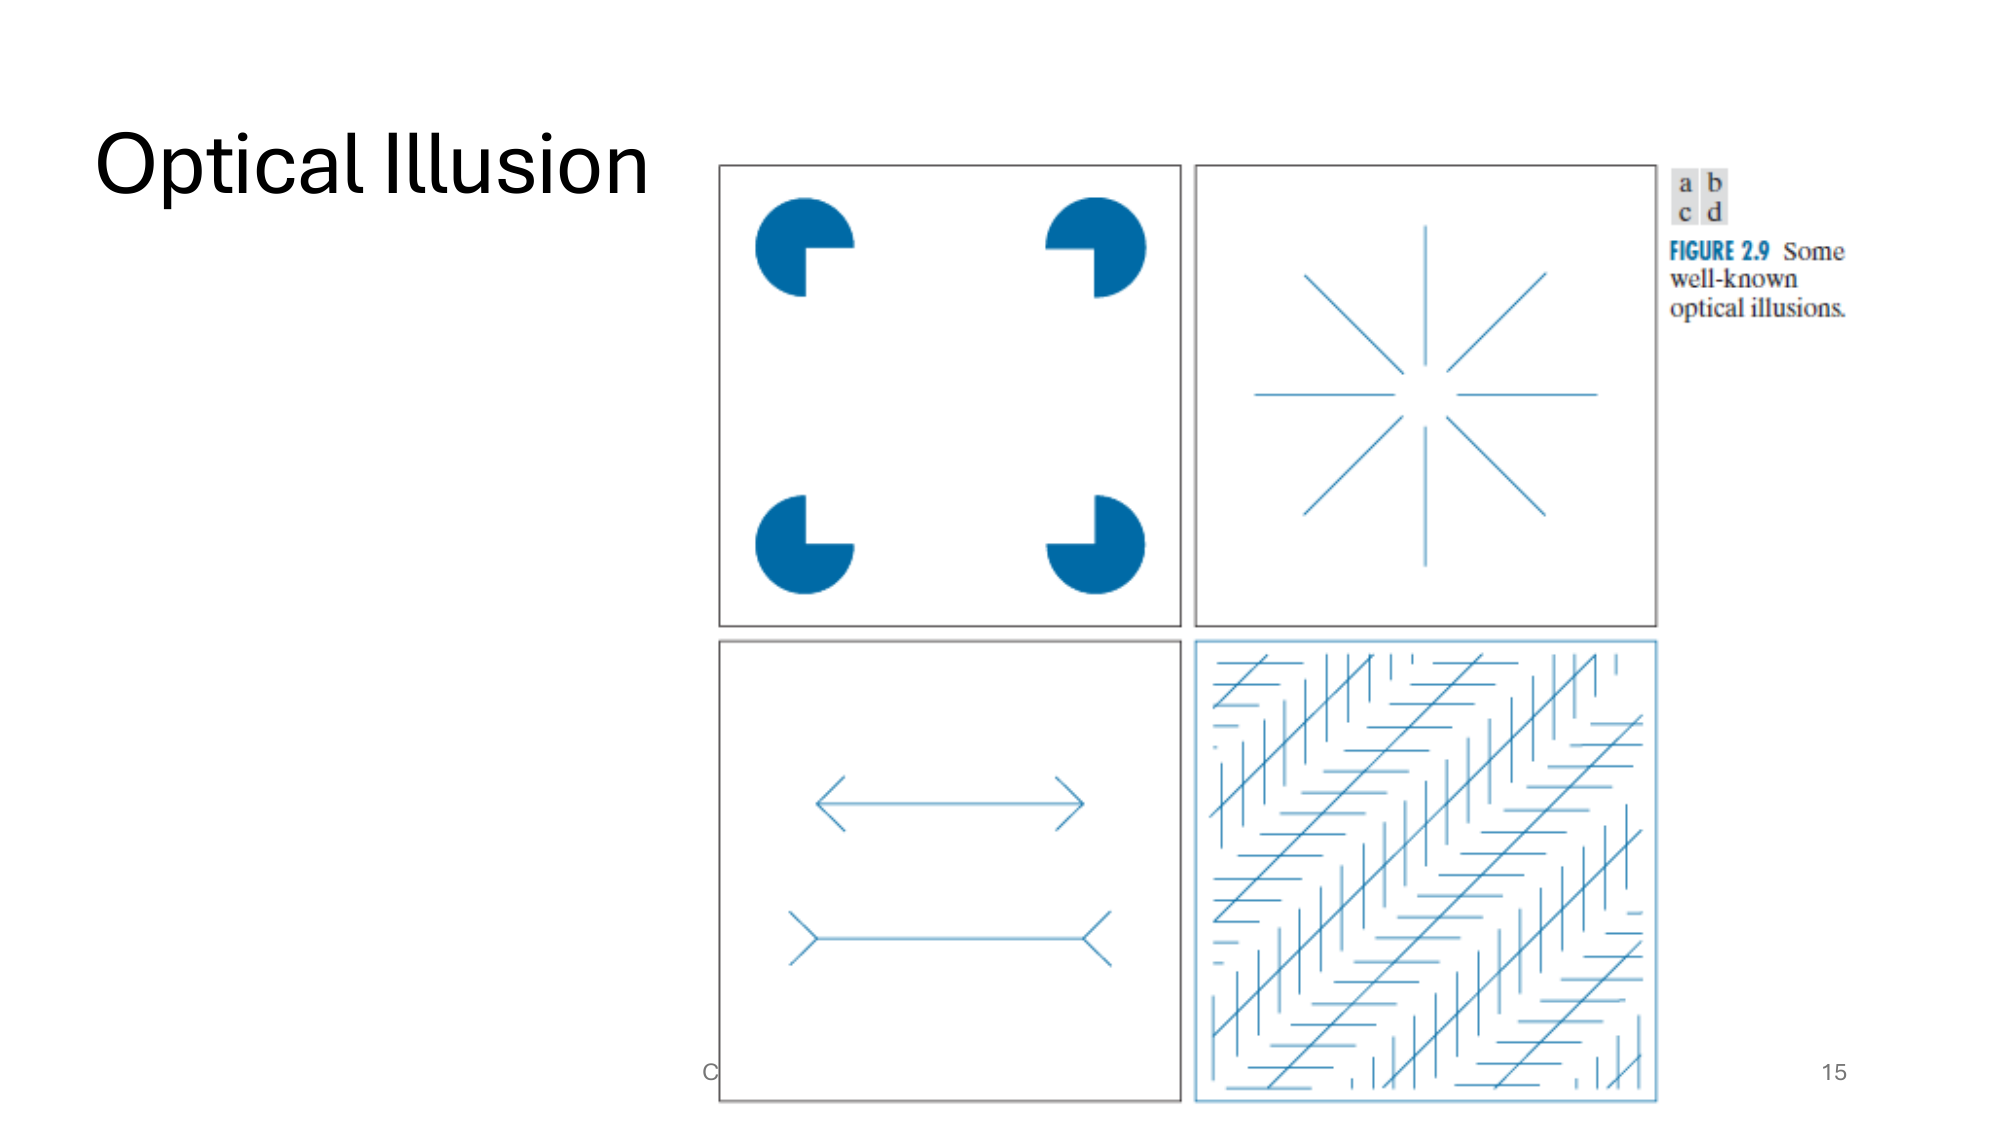
\includegraphics[width=0.85\textwidth]{images/slide2-15.png}
    \caption{Optical illusions demonstrating visual system characteristics}
    \label{fig:optical_illusions}
\end{figure}

\begin{deepexplanation}
\textbf{DEEP ANALYSIS - Figure \ref{fig:optical_illusions}: What Illusions Teach Us}

\textbf{Common Types of Visual Illusions:}

\textbf{1. Geometric Illusions (Müller-Lyer, Ponzo, etc.):}
\begin{itemize}
    \item Lines of equal length appear different due to context
    \item Visual system uses context for depth/size estimation
    \item These heuristics usually help but can mislead
\end{itemize}

\textbf{2. Motion Illusions:}
\begin{itemize}
    \item Static patterns appear to move
    \item Exploits motion detection circuits in visual cortex
\end{itemize}

\textbf{3. Brightness Illusions (Hermann Grid, etc.):}
\begin{itemize}
    \item Gray spots appear at intersections of white grid on black
    \item Caused by lateral inhibition in receptive fields
\end{itemize}

\textbf{Why Study Illusions?}
\begin{itemize}
    \item They reveal the \textbf{assumptions} built into visual processing
    \item Help us understand what image features the visual system emphasizes
    \item Guide design of more effective visualizations
    \item Explain why certain image artifacts are more/less noticeable
\end{itemize}

\textbf{Application to Image Processing:}
\begin{itemize}
    \item Compression exploits perceptual limitations (JPEG uses knowledge of contrast sensitivity)
    \item Image quality metrics should correlate with human perception
    \item Display technology must account for visual phenomena
\end{itemize}
\end{deepexplanation}

\subsection{Light and the Electromagnetic Spectrum}

\begin{figure}[H]
    \centering
    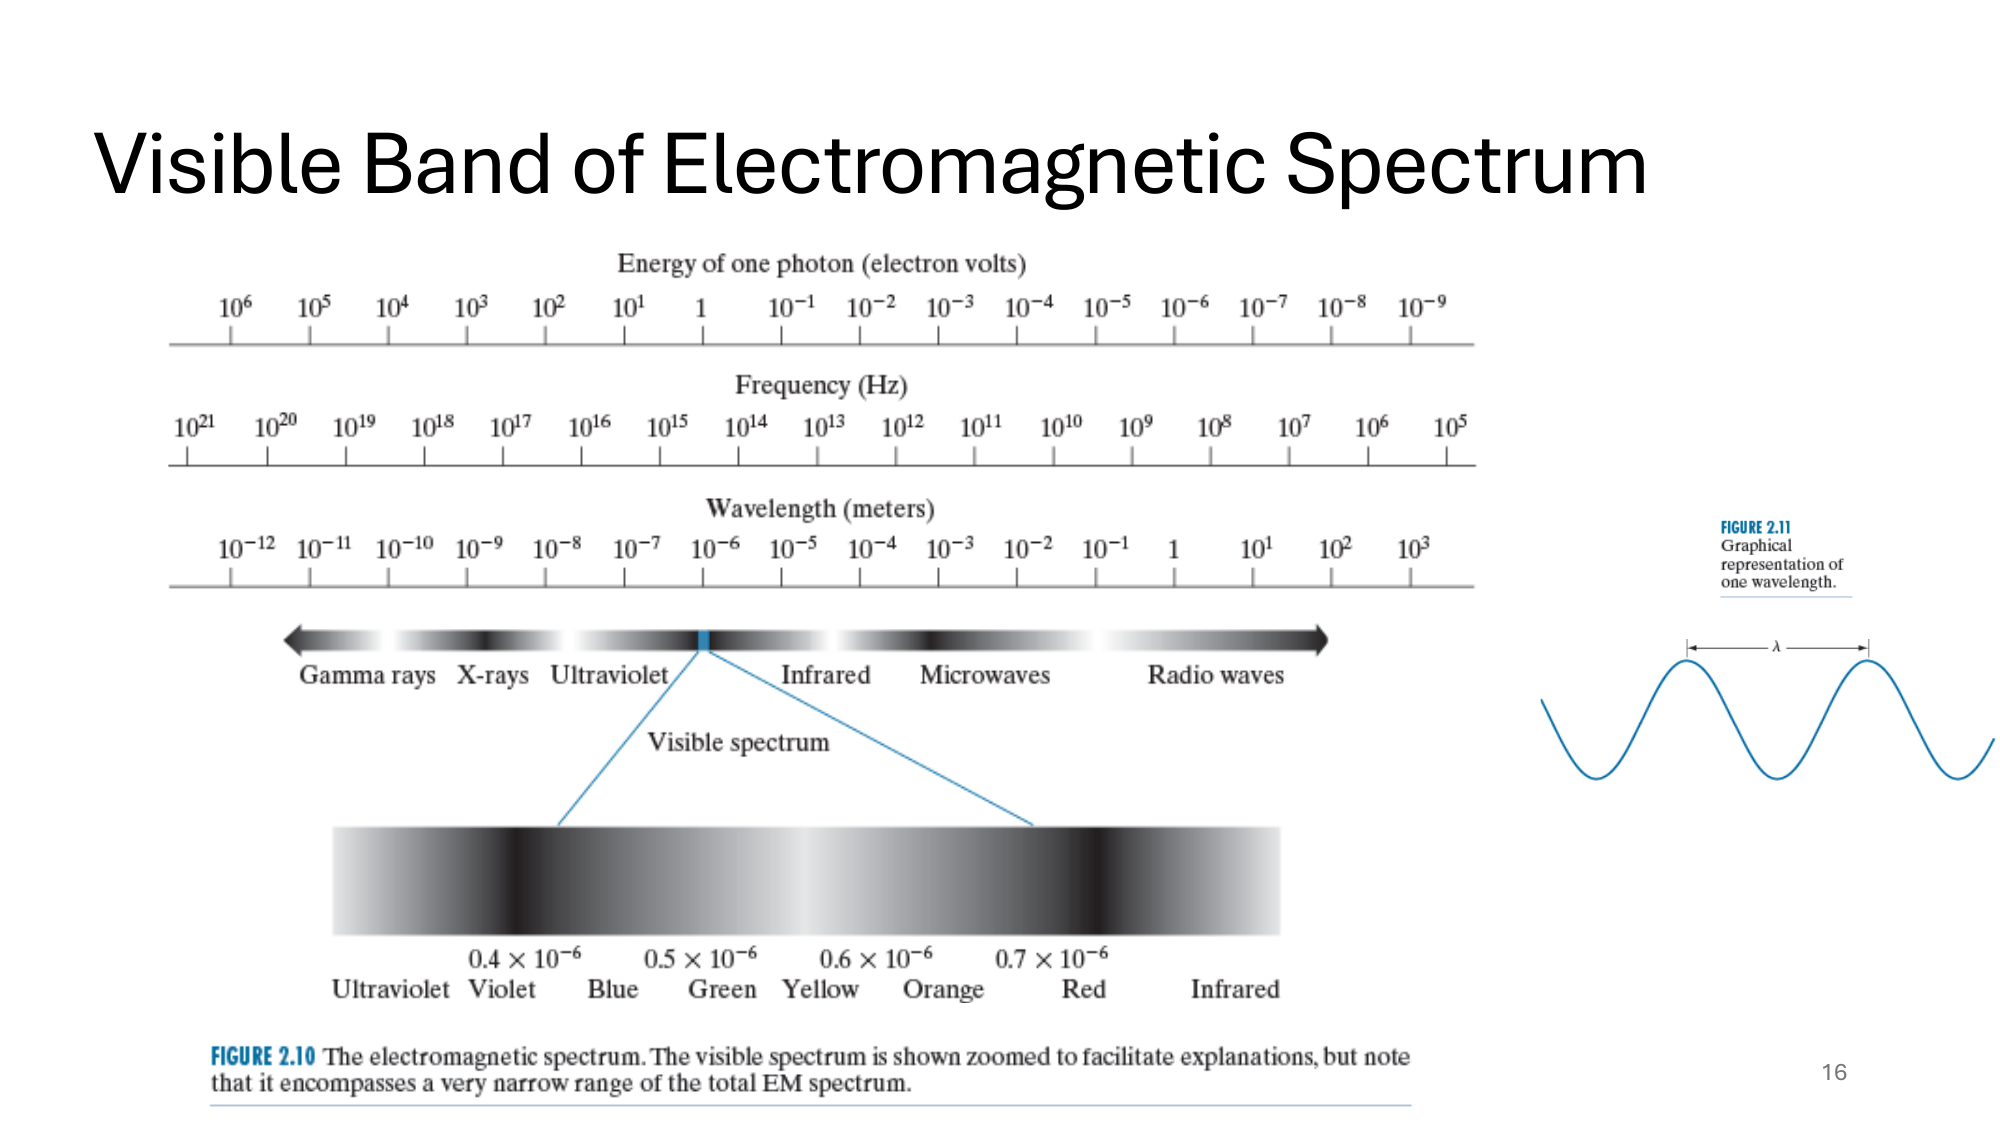
\includegraphics[width=0.9\textwidth]{images/slide2-16.png}
    \caption{The electromagnetic spectrum with visible light highlighted}
    \label{fig:em_spectrum}
\end{figure}

\begin{deepexplanation}
\textbf{DEEP ANALYSIS - Figure \ref{fig:em_spectrum}: Light in the EM Spectrum}

\textbf{The Full Electromagnetic Spectrum:}
\begin{center}
\begin{tabular}{|l|l|l|}
\hline
\textbf{Region} & \textbf{Wavelength} & \textbf{Imaging Application} \\
\hline
Gamma rays & $< 0.01$ nm & Medical (PET), nuclear inspection \\
X-rays & $0.01$--$10$ nm & Medical, security, materials \\
Ultraviolet & $10$--$400$ nm & Fluorescence, lithography \\
\textbf{Visible} & \textbf{400--700 nm} & \textbf{Photography, microscopy} \\
Near Infrared & $700$ nm--$1$ µm & Night vision, communication \\
Thermal IR & $3$--$15$ µm & Thermal imaging, remote sensing \\
Microwave & $1$ mm--$1$ m & Radar, SAR imaging \\
Radio & $> 1$ m & Radio astronomy, MRI \\
\hline
\end{tabular}
\end{center}

\textbf{Visible Light Details:}
\begin{itemize}
    \item Violet: $\approx 400$--$450$ nm
    \item Blue: $\approx 450$--$495$ nm
    \item Green: $\approx 495$--$570$ nm
    \item Yellow: $\approx 570$--$590$ nm
    \item Orange: $\approx 590$--$620$ nm
    \item Red: $\approx 620$--$700$ nm
\end{itemize}

\textbf{Key Physical Relationships:}
\[
c = \lambda \cdot \nu, \quad E = h\nu = \frac{hc}{\lambda}
\]
where $c$ = speed of light, $\lambda$ = wavelength, $\nu$ = frequency, $h$ = Planck's constant.

Shorter wavelength $\rightarrow$ higher frequency $\rightarrow$ higher energy.

\textbf{Why Wavelength Matters for Imaging:}
\begin{itemize}
    \item To ``see'' an object, wavelength must be $\leq$ object size
    \item Visible light: Can image features $\geq 200$ nm (diffraction limit)
    \item X-rays needed for atomic/molecular scale
    \item Different wavelengths reveal different information (multispectral imaging)
\end{itemize}
\end{deepexplanation}

\subsection{Radiometric Quantities}

\begin{figure}[H]
    \centering
    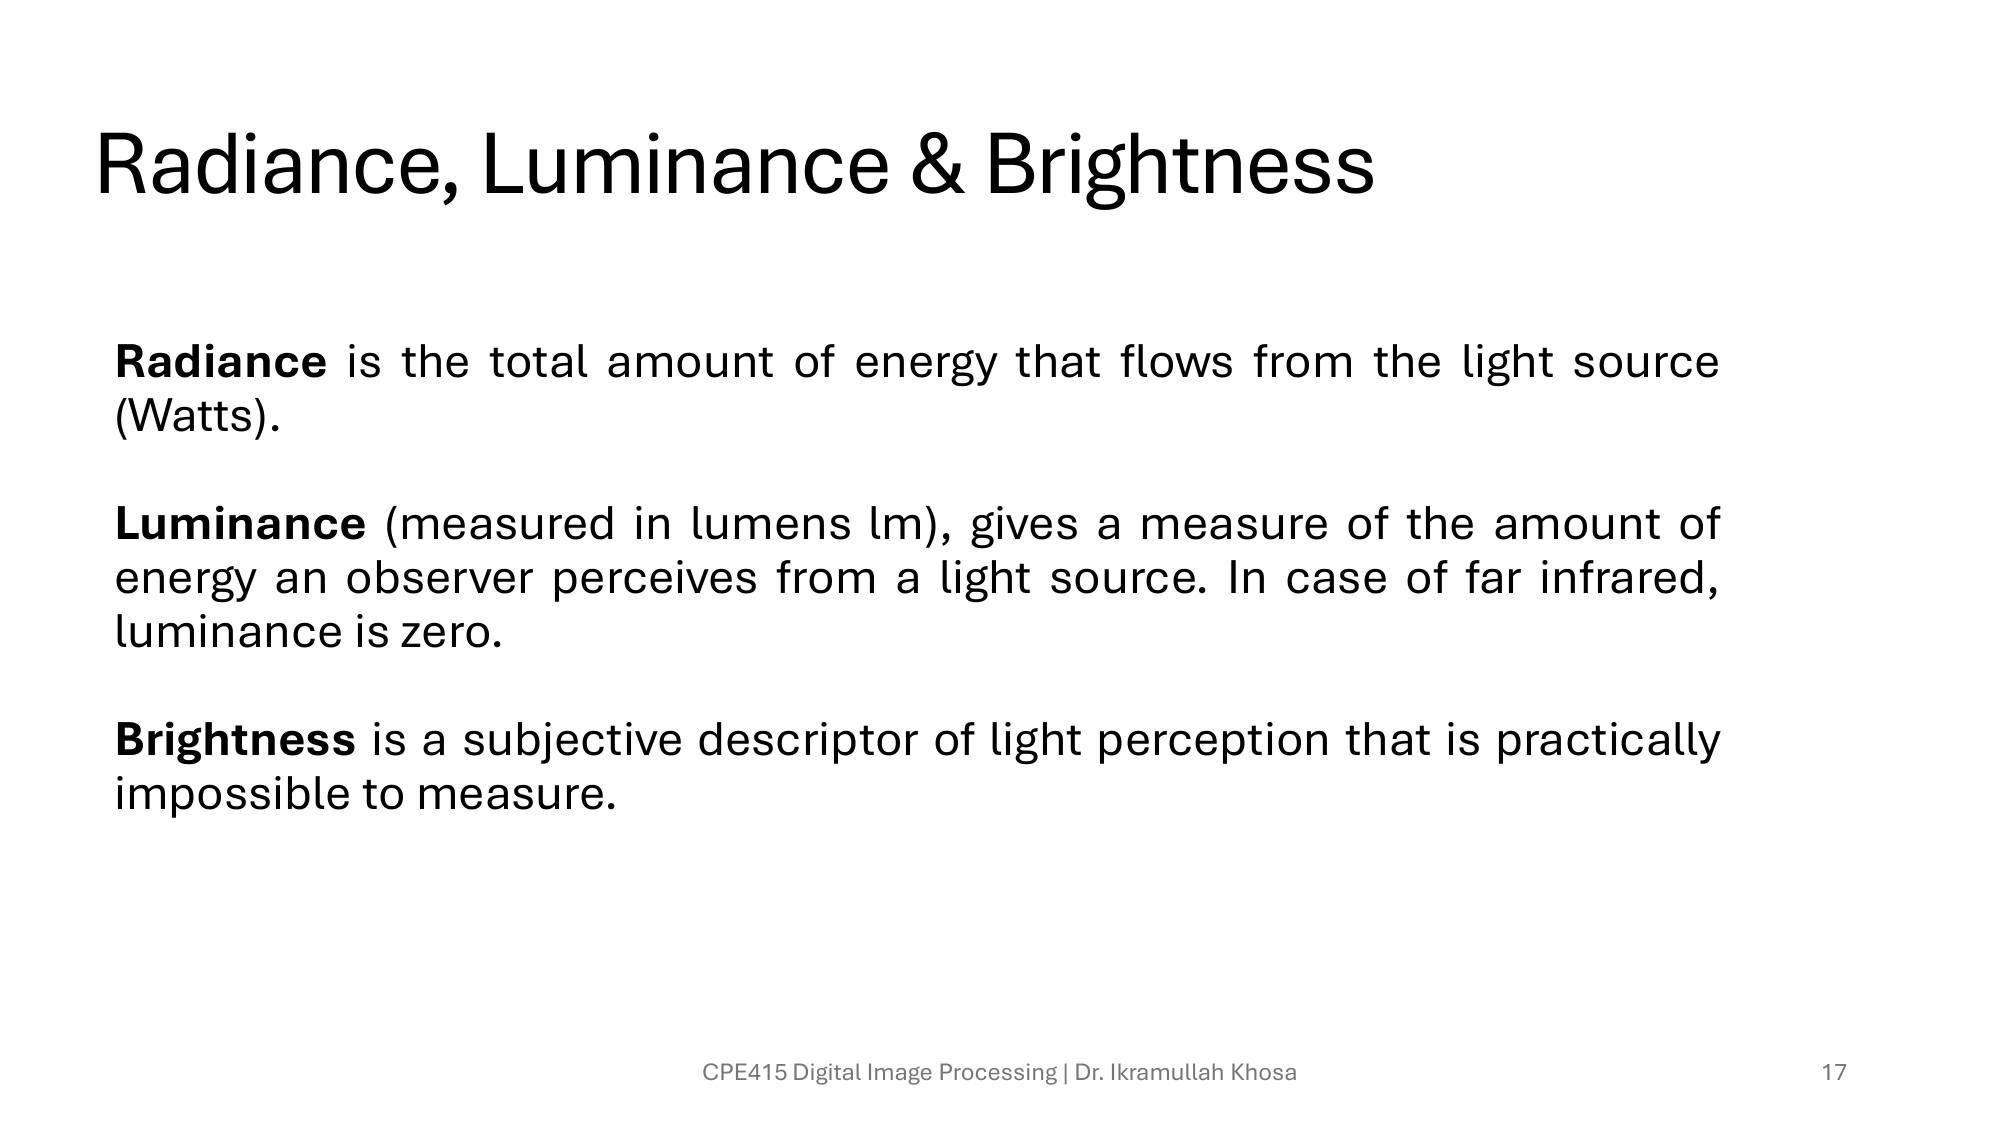
\includegraphics[width=0.85\textwidth]{images/slide2-17.png}
    \caption{Radiance, luminance, and brightness definitions}
    \label{fig:radiometric}
\end{figure}

\begin{deepexplanation}
\textbf{DEEP ANALYSIS - Figure \ref{fig:radiometric}: Measuring Light}

\textbf{Three Related but Distinct Quantities:}

\textbf{1. Radiance (Physical --- Watts):}
\begin{itemize}
    \item Total power (energy/time) emitted or reflected by a source
    \item Measured in Watts (W) or W/m²/sr (per area per solid angle)
    \item \textbf{Objective}: Can be measured with instruments
    \item Includes all wavelengths, even those invisible to humans
\end{itemize}

\textbf{2. Luminance (Perceptual-Weighted --- Lumens):}
\begin{itemize}
    \item Radiance weighted by human eye sensitivity $V(\lambda)$
    \item Measured in lumens (lm) or candela/m² (cd/m²)
    \item Accounts for wavelength-dependent sensitivity (peak at $\approx 555$ nm, green)
    \item Far-infrared has zero luminance (we can't see it)
\end{itemize}

\textbf{3. Brightness (Subjective):}
\begin{itemize}
    \item Perceived intensity --- what you ``see''
    \item Cannot be directly measured (subjective experience)
    \item Affected by adaptation, context, surrounding intensities
    \item Related to luminance but not linearly
\end{itemize}

\textbf{The Relationship:}
\[
\text{Brightness} \propto (\text{Luminance})^{1/3} \text{ to } (\text{Luminance})^{1/2}
\]
(Approximately --- varies with conditions)

\textbf{Why This Matters:}
\begin{itemize}
    \item Camera sensors measure radiance (or approximation)
    \item Display brightness should match luminance perception
    \item Gamma correction bridges physical and perceptual domains
\end{itemize}
\end{deepexplanation}


%==============================================================================
\section{Image Sensing and Acquisition}
%==============================================================================

\subsection{Image Formation Model}

\begin{conceptbox}[The Fundamental Image Formation Equation]
\[
f(x,y) = i(x,y) \cdot r(x,y)
\]
where:
\begin{itemize}
    \item $f(x,y)$ = image intensity (what the sensor records)
    \item $i(x,y)$ = \textbf{illumination} (light falling on the scene) --- $0 < i(x,y) < \infty$
    \item $r(x,y)$ = \textbf{reflectance} (fraction of light reflected by surface) --- $0 < r(x,y) < 1$
\end{itemize}
\end{conceptbox}

\begin{figure}[H]
    \centering
    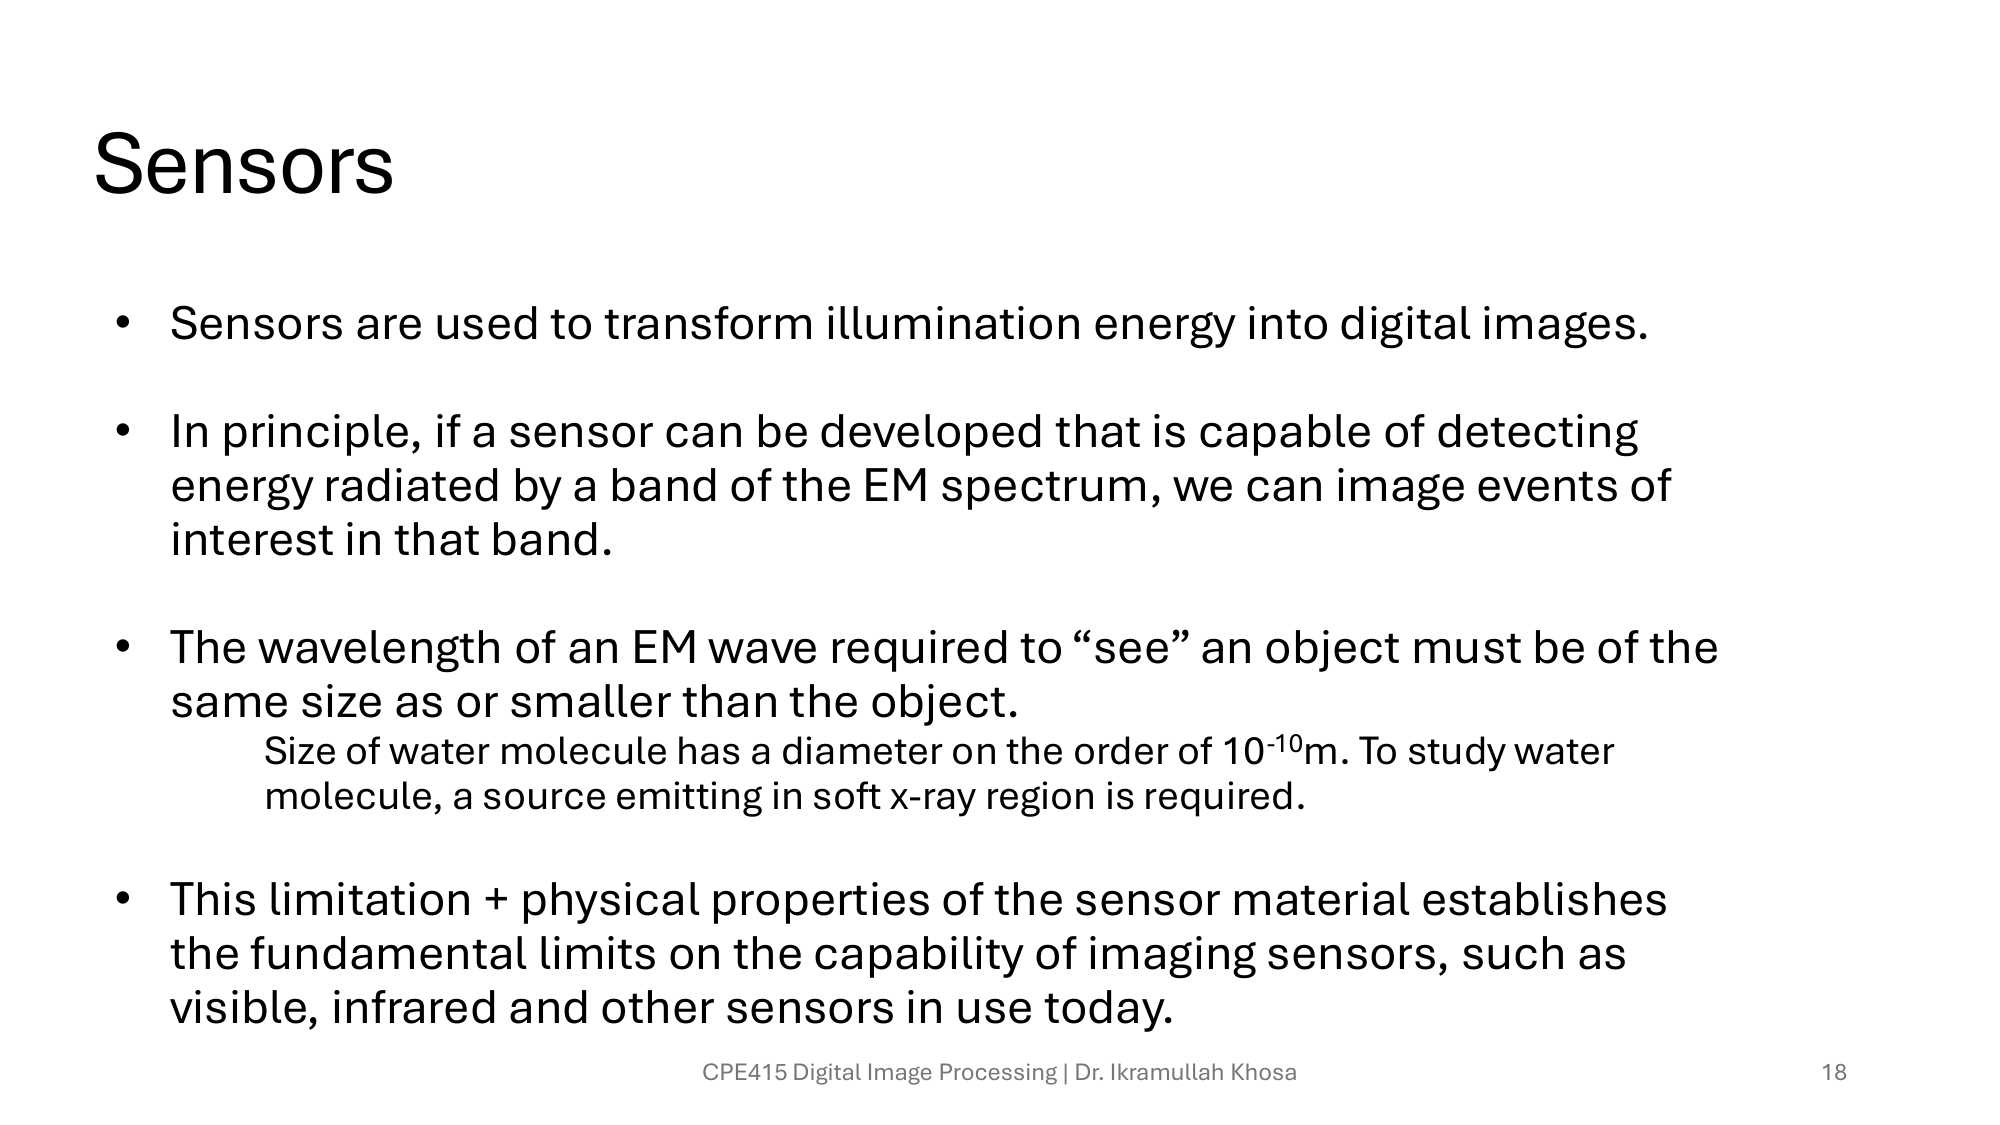
\includegraphics[width=0.85\textwidth]{images/slide2-18.png}
    \caption{Single sensor image acquisition}
    \label{fig:single_sensor}
\end{figure}

\begin{deepexplanation}
\textbf{DEEP ANALYSIS - Figure \ref{fig:single_sensor}: The Simplest Image Acquisition}

\textbf{Single Sensor Configuration:}
A single photodetector (e.g., photodiode) can only measure one intensity value at a time. To form an image:

\textbf{1. Mechanical Scanning:}
\begin{itemize}
    \item Move the sensor (or object) in a raster pattern
    \item At each position, record one intensity value
    \item Extremely slow but high precision possible
    \item Used in: Drum scanners, some satellite sensors
\end{itemize}

\textbf{2. Component Parts:}
\begin{itemize}
    \item \textbf{Filter}: Selects wavelength range (optical bandpass)
    \item \textbf{Lens}: Focuses light onto the sensor
    \item \textbf{Sensor}: Converts photons to electrical signal (photoelectric effect)
\end{itemize}

\textbf{Photoelectric Effect:}
\[
\text{Signal voltage} \propto \int_0^T I(t) \, dt
\]
where $T$ = exposure time, $I(t)$ = instantaneous light intensity.

\textbf{Limitations:}
\begin{itemize}
    \item Speed: Scanning takes time
    \item Moving parts: Mechanical complexity
    \item For 2D images: Need motion in both x and y
\end{itemize}

\textbf{Modern Use Cases:}
\begin{itemize}
    \item Flatbed scanners (single linear array + motion)
    \item Push-broom satellite sensors (linear array + spacecraft motion)
    \item Confocal microscopy (point-by-point scanning)
\end{itemize}
\end{deepexplanation}

\begin{figure}[H]
    \centering
    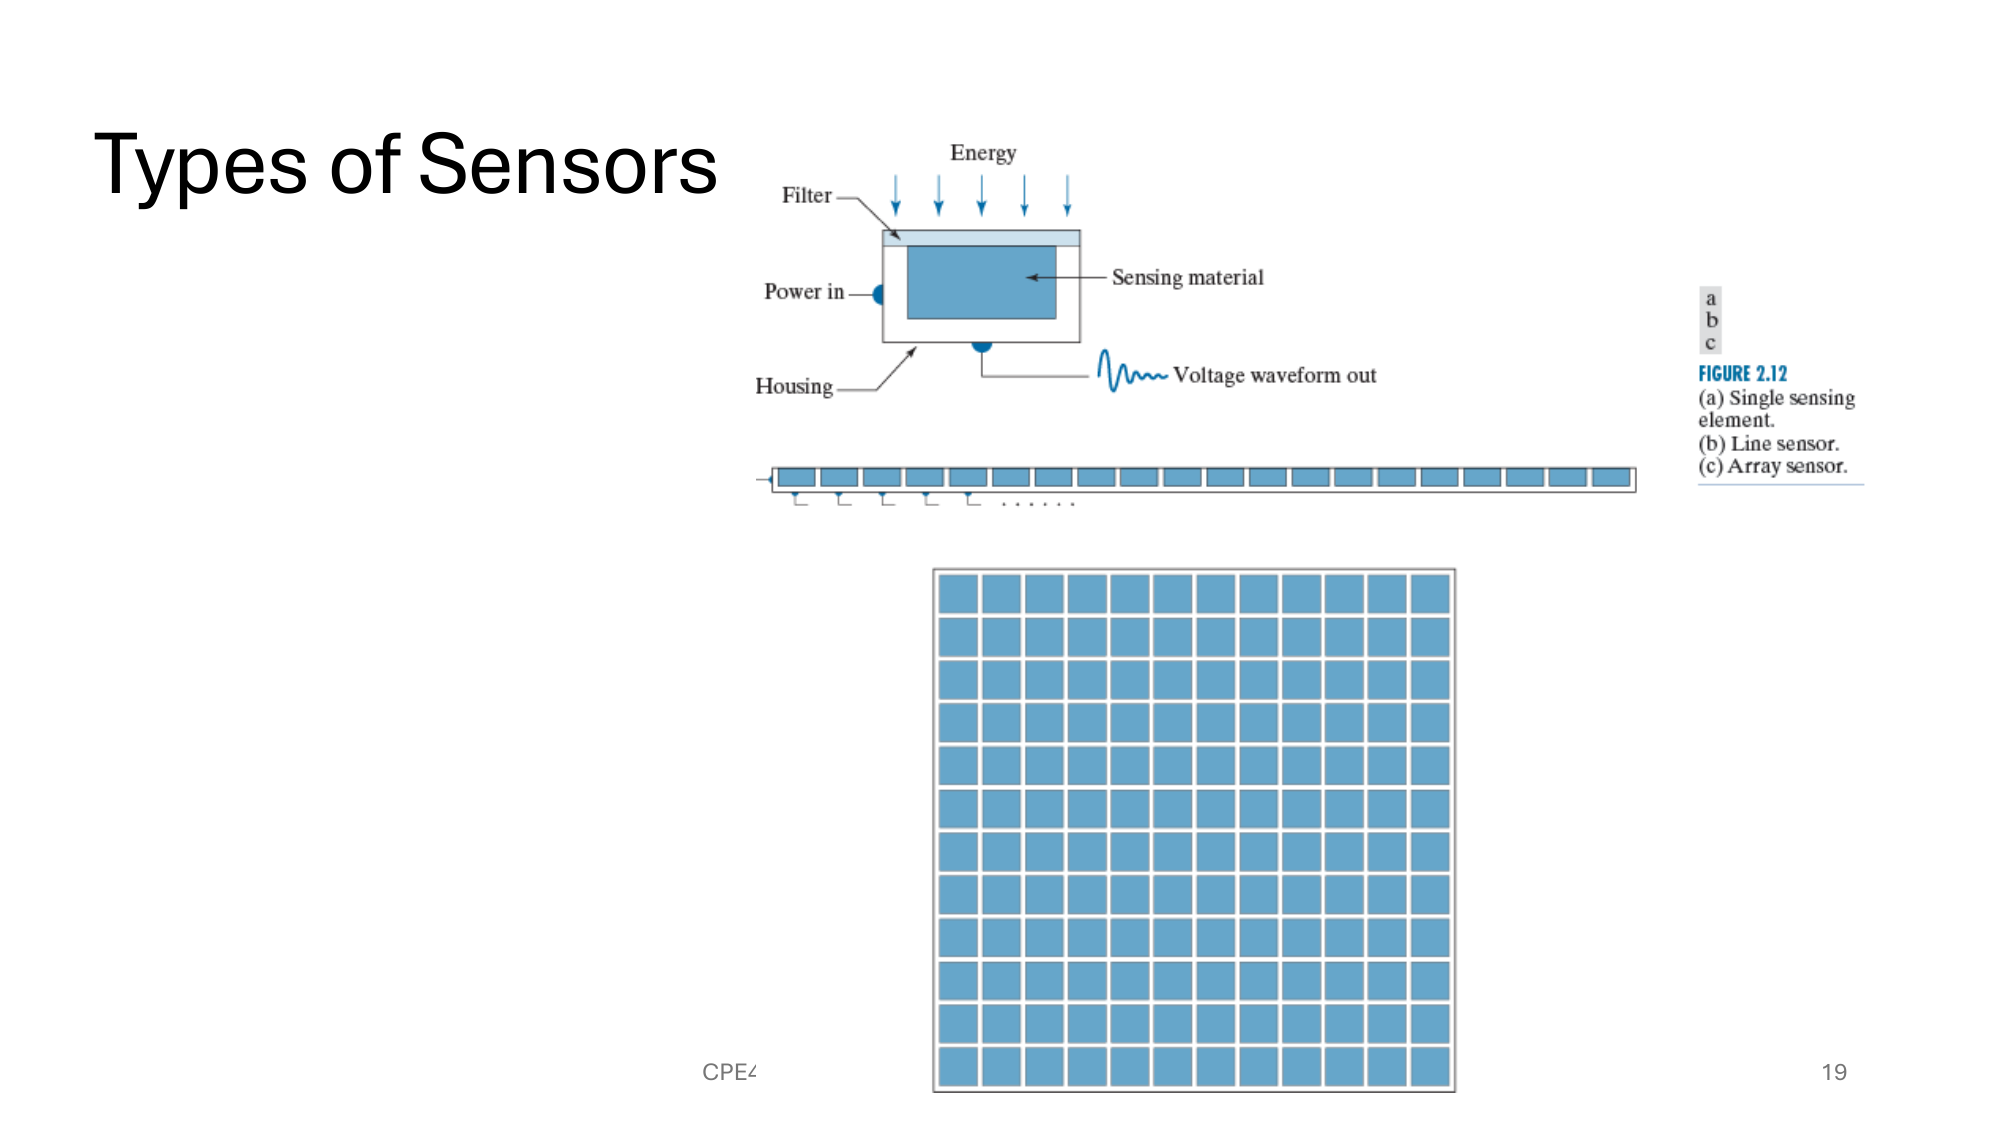
\includegraphics[width=0.85\textwidth]{images/slide2-19.png}
    \caption{Line sensor (linear array) image acquisition}
    \label{fig:line_sensor}
\end{figure}

\begin{deepexplanation}
\textbf{DEEP ANALYSIS - Figure \ref{fig:line_sensor}: Linear Array Sensors}

\textbf{How It Works:}
\begin{itemize}
    \item A row of individual sensors arranged in a line
    \item Captures one entire line of the image simultaneously
    \item Need only 1D motion (perpendicular to the array) to build 2D image
\end{itemize}

\textbf{Resolution Considerations:}
If the array has $N$ sensors and spans physical width $W$:
\begin{itemize}
    \item Sensor pitch: $p = W/N$
    \item Maximum spatial frequency: $f_{max} = 1/(2p)$ (Nyquist)
    \item Typical arrays: 4096--12000+ elements
\end{itemize}

\textbf{Applications:}
\begin{itemize}
    \item \textbf{Document scanners}: Page moves under fixed linear sensor
    \item \textbf{Satellite imaging}: Spacecraft motion provides ``scan''
    \item \textbf{Industrial inspection}: Products on conveyor belt
    \item \textbf{Barcode readers}: Linear array reads stripes
\end{itemize}

\textbf{Advantages over Single Sensor:}
\begin{itemize}
    \item Much faster (capture entire line at once)
    \item Only 1D motion required
    \item Good compromise between speed and complexity
\end{itemize}

\textbf{Comparison:}
\begin{center}
\begin{tabular}{|l|c|c|c|}
\hline
\textbf{Type} & \textbf{Speed} & \textbf{Cost} & \textbf{Motion} \\
\hline
Single sensor & Slowest & Lowest & 2D \\
Linear array & Medium & Medium & 1D \\
Area array & Fastest & Highest & None \\
\hline
\end{tabular}
\end{center}
\end{deepexplanation}

\begin{figure}[H]
    \centering
    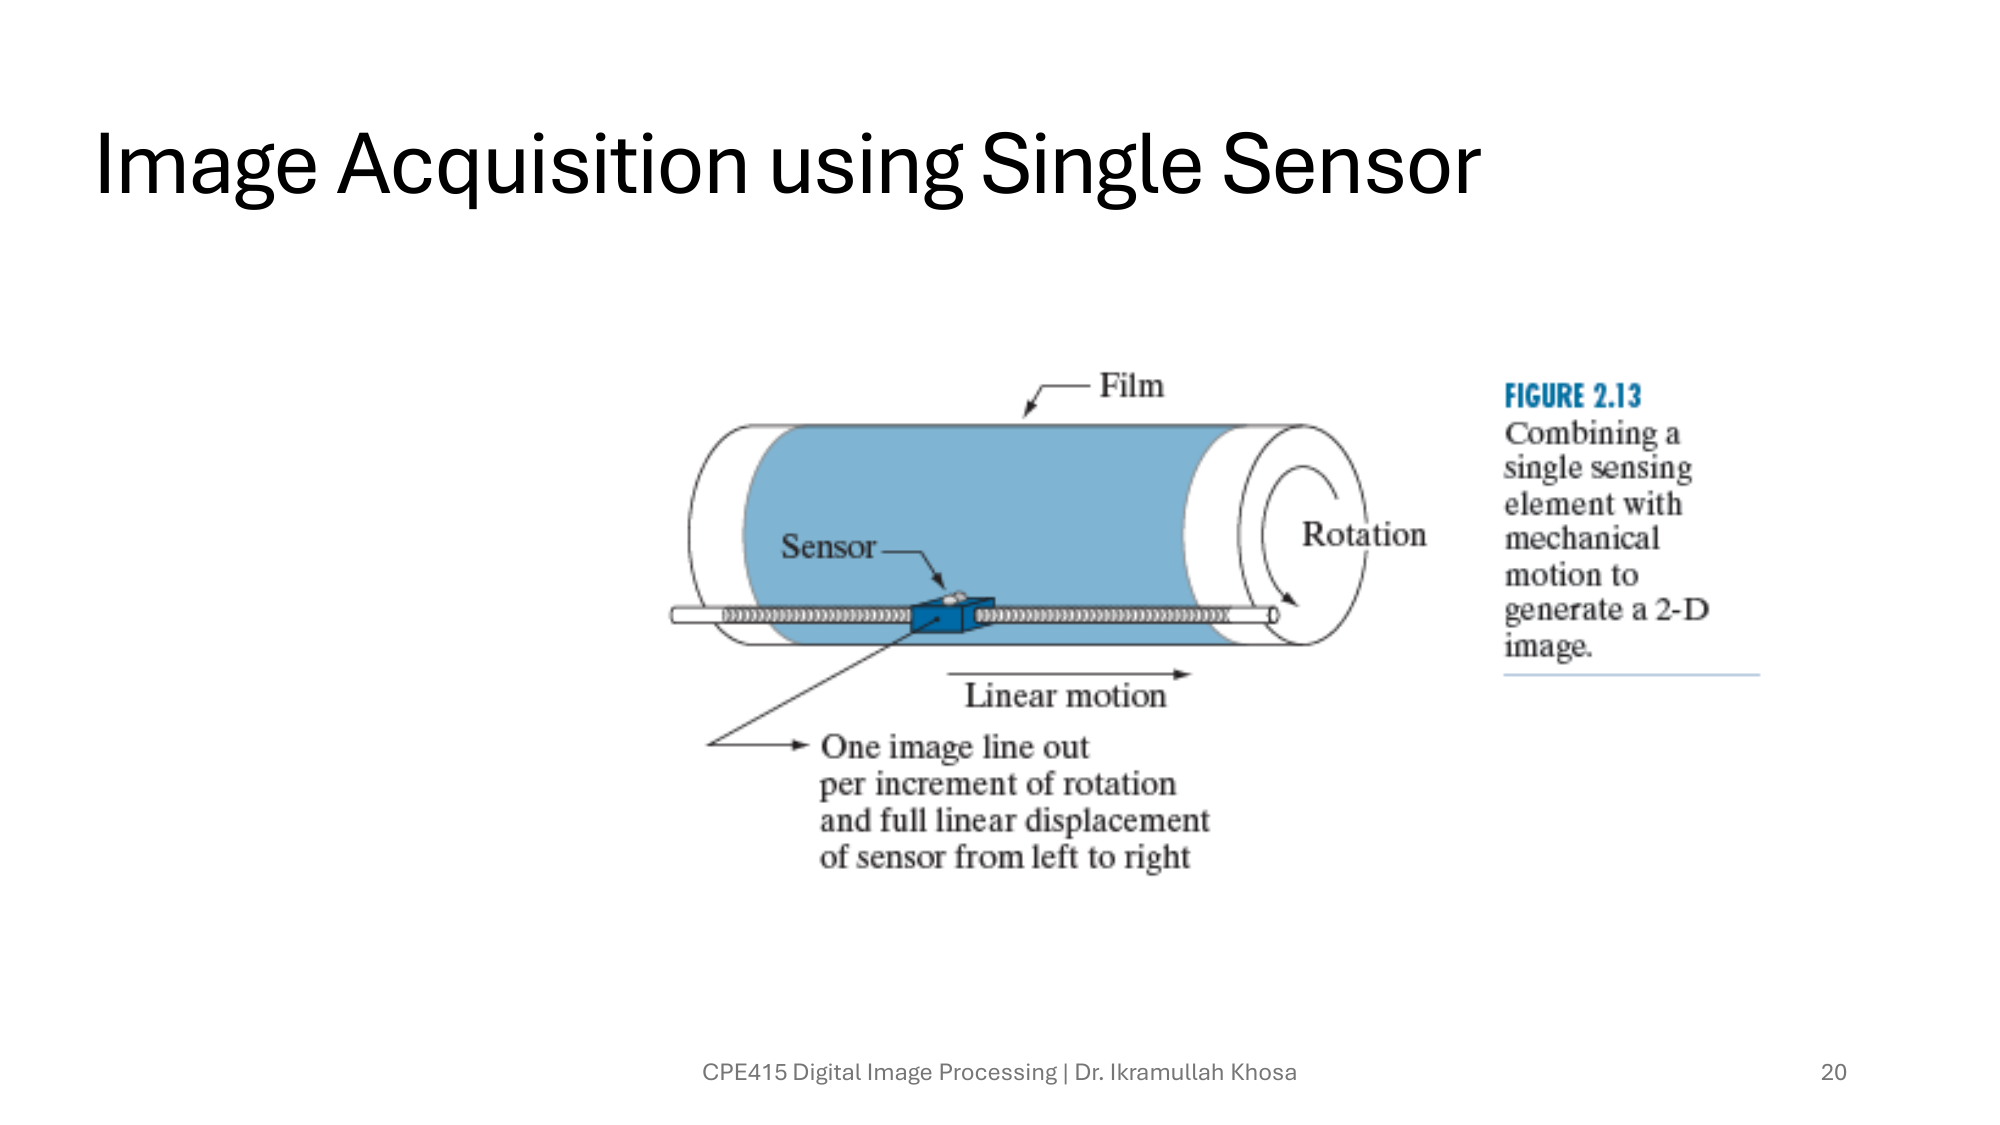
\includegraphics[width=0.85\textwidth]{images/slide2-20.png}
    \caption{2D array sensor for instantaneous image capture}
    \label{fig:array_sensor}
\end{figure}

\begin{deepexplanation}
\textbf{DEEP ANALYSIS - Figure \ref{fig:array_sensor}: 2D Area Array Sensors}

\textbf{The Technology:}
\begin{itemize}
    \item Grid of photosensitive elements (pixels)
    \item Captures entire image in one exposure
    \item Two main technologies: CCD and CMOS
\end{itemize}

\textbf{CCD (Charge-Coupled Device):}
\begin{enumerate}
    \item Photons generate electrons in each pixel
    \item Charges are shifted row-by-row to readout register
    \item Serial readout through single amplifier
    \item \textbf{Pros}: Uniform response, low noise
    \item \textbf{Cons}: Slow readout, high power, specialized fabrication
\end{enumerate}

\textbf{CMOS (Active Pixel Sensor):}
\begin{enumerate}
    \item Each pixel has its own amplifier and readout circuit
    \item Random access possible (read any pixel)
    \item Parallel readout through column buses
    \item \textbf{Pros}: Fast, low power, integrable with other circuits
    \item \textbf{Cons}: More noise (historically), fixed pattern noise
\end{enumerate}

\textbf{Resolution Examples:}
\begin{itemize}
    \item Smartphone: 12--108 megapixels
    \item DSLR: 24--60 megapixels
    \item Medium format: 100+ megapixels
    \item Scientific: $4k \times 4k$ is common
\end{itemize}

\textbf{Fill Factor:}
Not all pixel area is light-sensitive:
\[
\text{Fill factor} = \frac{\text{Photosensitive area}}{\text{Total pixel area}}
\]
Microlenses improve effective fill factor in modern sensors.
\end{deepexplanation}

\begin{figure}[H]
    \centering
    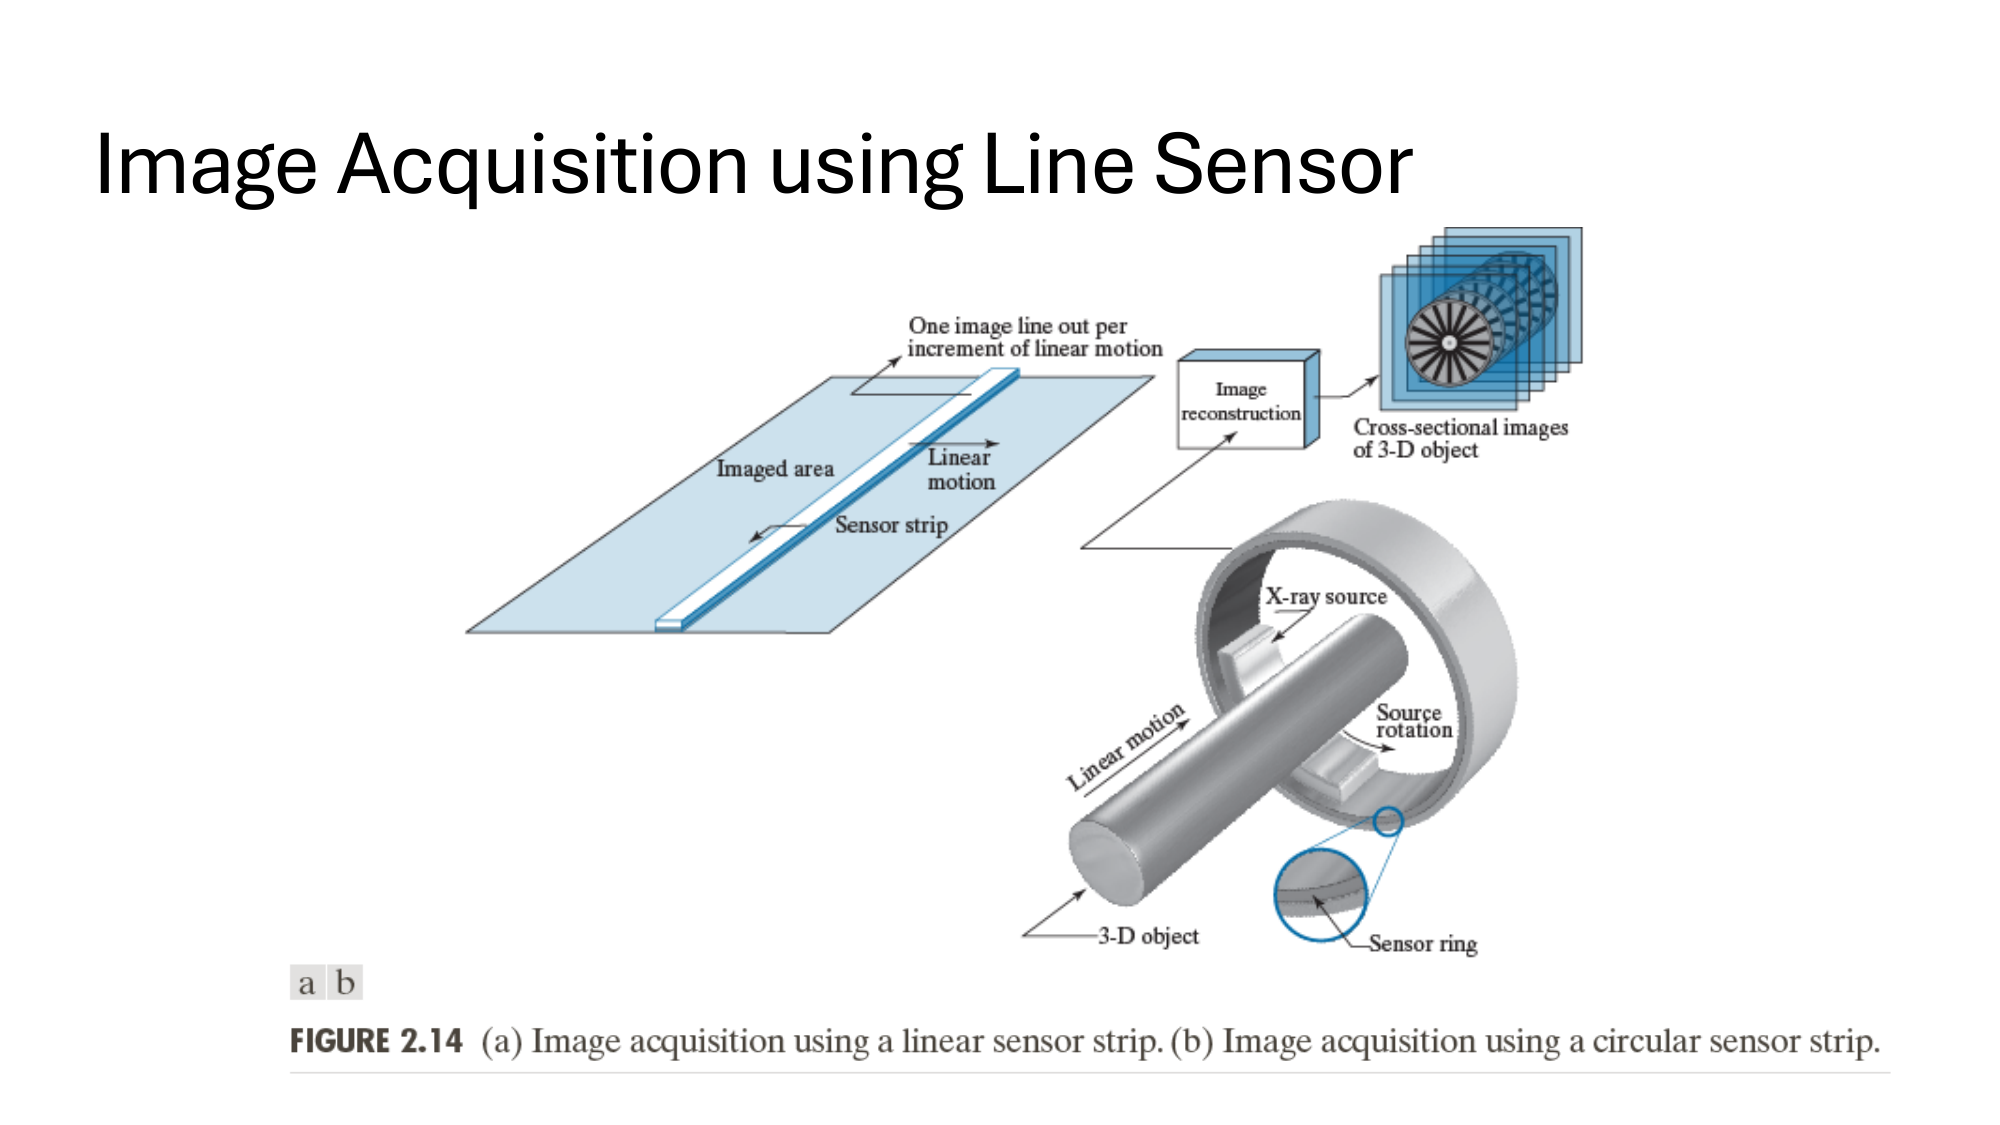
\includegraphics[width=0.85\textwidth]{images/slide2-21.png}
    \caption{Simple image acquisition process}
    \label{fig:acquisition_process}
\end{figure}

\begin{figure}[H]
    \centering
    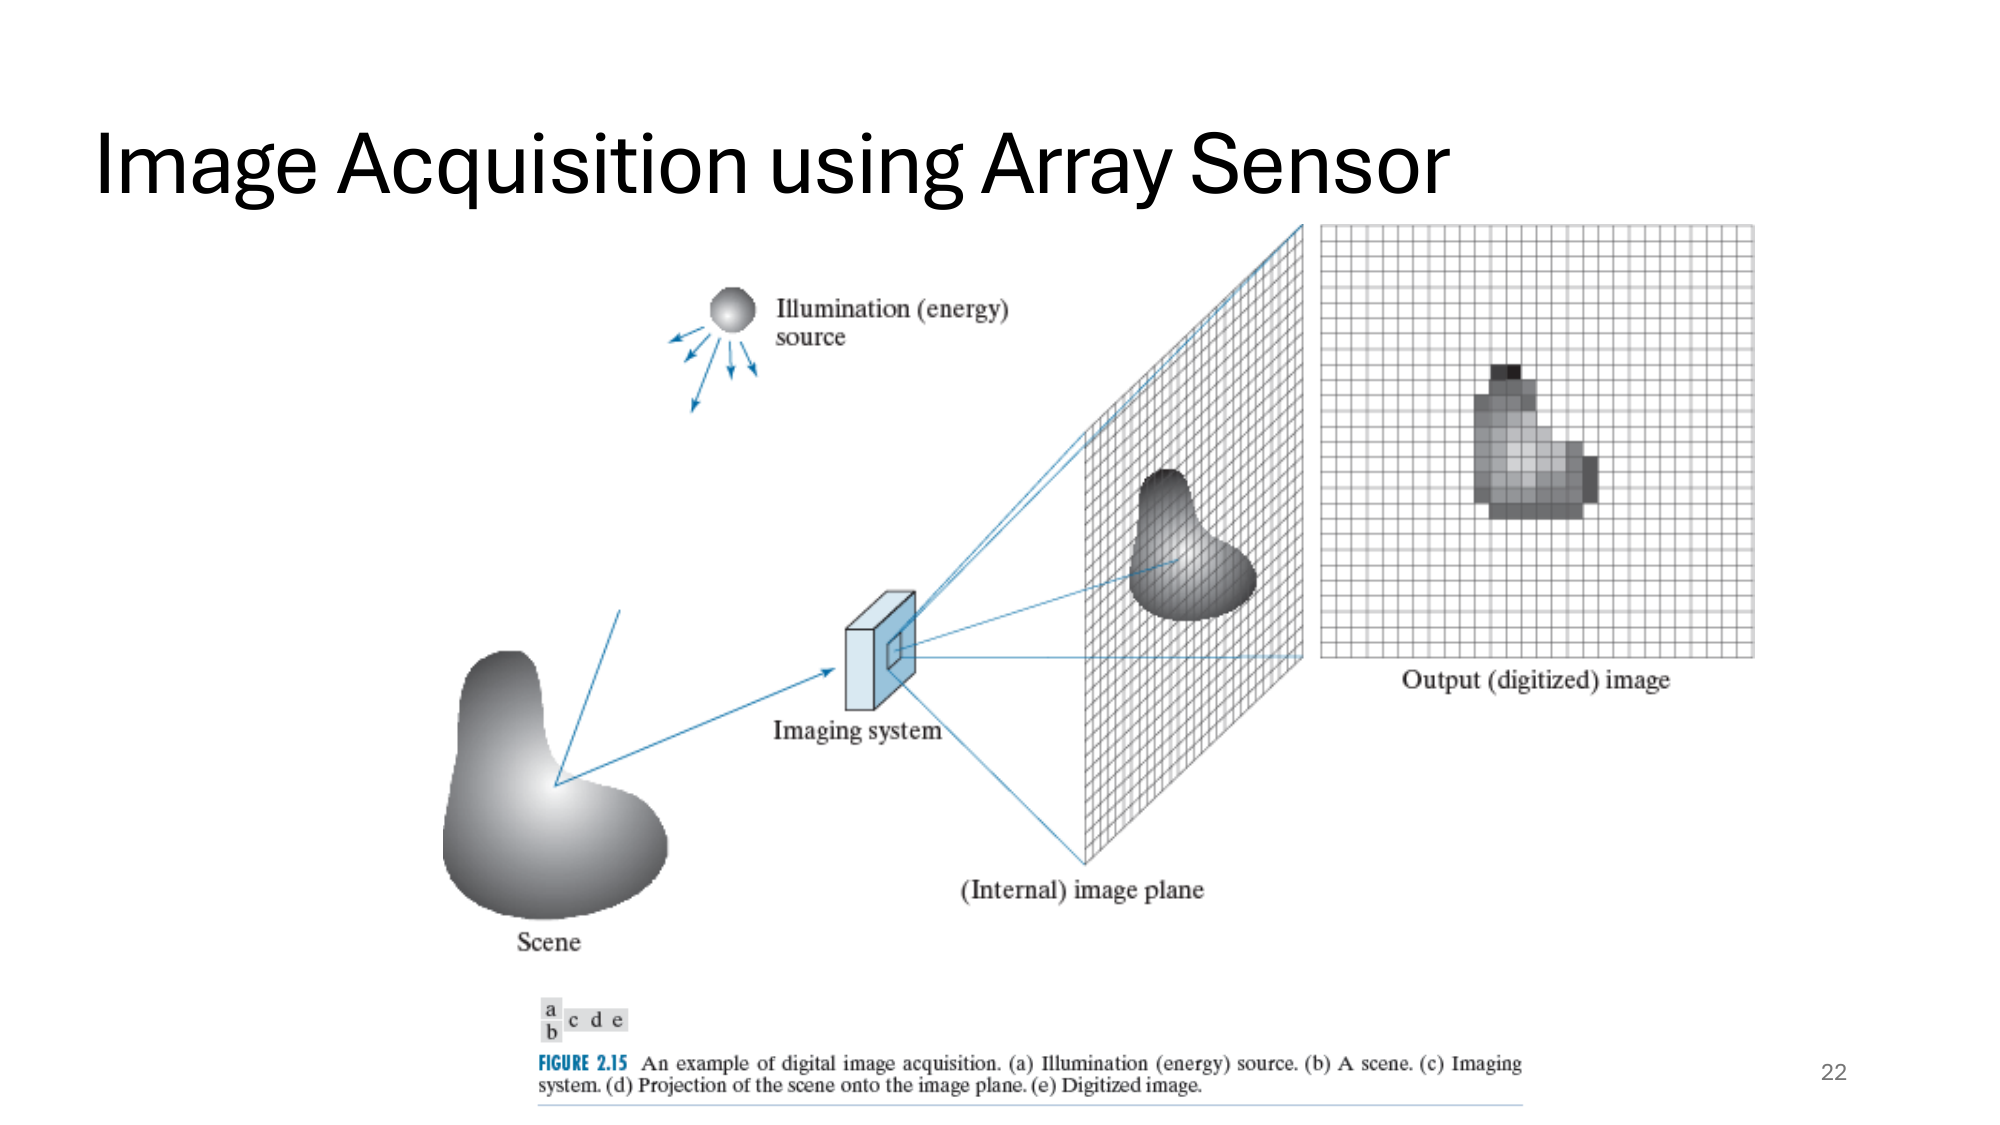
\includegraphics[width=0.85\textwidth]{images/slide2-22.png}
    \caption{Illumination and reflectance model}
    \label{fig:illumination_reflectance}
\end{figure}

\begin{deepexplanation}
\textbf{DEEP ANALYSIS - Figure \ref{fig:illumination_reflectance}: Separating Illumination and Reflectance}

\textbf{The Multiplicative Model:}
\[
f(x,y) = i(x,y) \cdot r(x,y)
\]

\textbf{Physical Interpretation:}
\begin{itemize}
    \item \textbf{Illumination} $i(x,y)$: Determined by light source(s)
    \begin{itemize}
        \item Varies slowly (smooth) --- typically low spatial frequency
        \item Indoor: $100$--$1000$ lux typical
        \item Outdoor: $10,000$--$100,000$ lux (sunlight)
    \end{itemize}
    \item \textbf{Reflectance} $r(x,y)$: Property of the object surface
    \begin{itemize}
        \item Can vary rapidly (edges, textures) --- high spatial frequency
        \item Black velvet: $r \approx 0.01$ (1\%)
        \item White paper: $r \approx 0.90$ (90\%)
        \item Snow: $r \approx 0.93$
        \item Human skin: $r \approx 0.35$--$0.50$
    \end{itemize}
\end{itemize}

\textbf{Why This Model Matters:}

\textbf{1. Homomorphic Filtering:}
Taking the logarithm:
\[
\ln f(x,y) = \ln i(x,y) + \ln r(x,y)
\]
Now it's \textbf{additive}! Can filter illumination and reflectance separately:
\begin{itemize}
    \item High-pass filter: Enhances reflectance (details)
    \item Low-pass filter: Smooths illumination
\end{itemize}

\textbf{2. Retinex Theory:}
Human vision uses a similar decomposition for color constancy.

\textbf{3. Shading Correction:}
If we know $i(x,y)$ (from a reference image), we can correct:
\[
r(x,y) = \frac{f(x,y)}{i(x,y)}
\]
\end{deepexplanation}

%==============================================================================
\section{Sampling and Quantization}
%==============================================================================

\subsection{The Digitization Process}

\begin{conceptbox}[From Continuous to Discrete]
Converting a continuous image to digital form requires two processes:
\begin{enumerate}
    \item \textbf{Sampling}: Discretizing the \textbf{spatial coordinates} $(x, y)$
    \item \textbf{Quantization}: Discretizing the \textbf{intensity values} (gray levels)
\end{enumerate}
\end{conceptbox}

\begin{figure}[H]
    \centering
    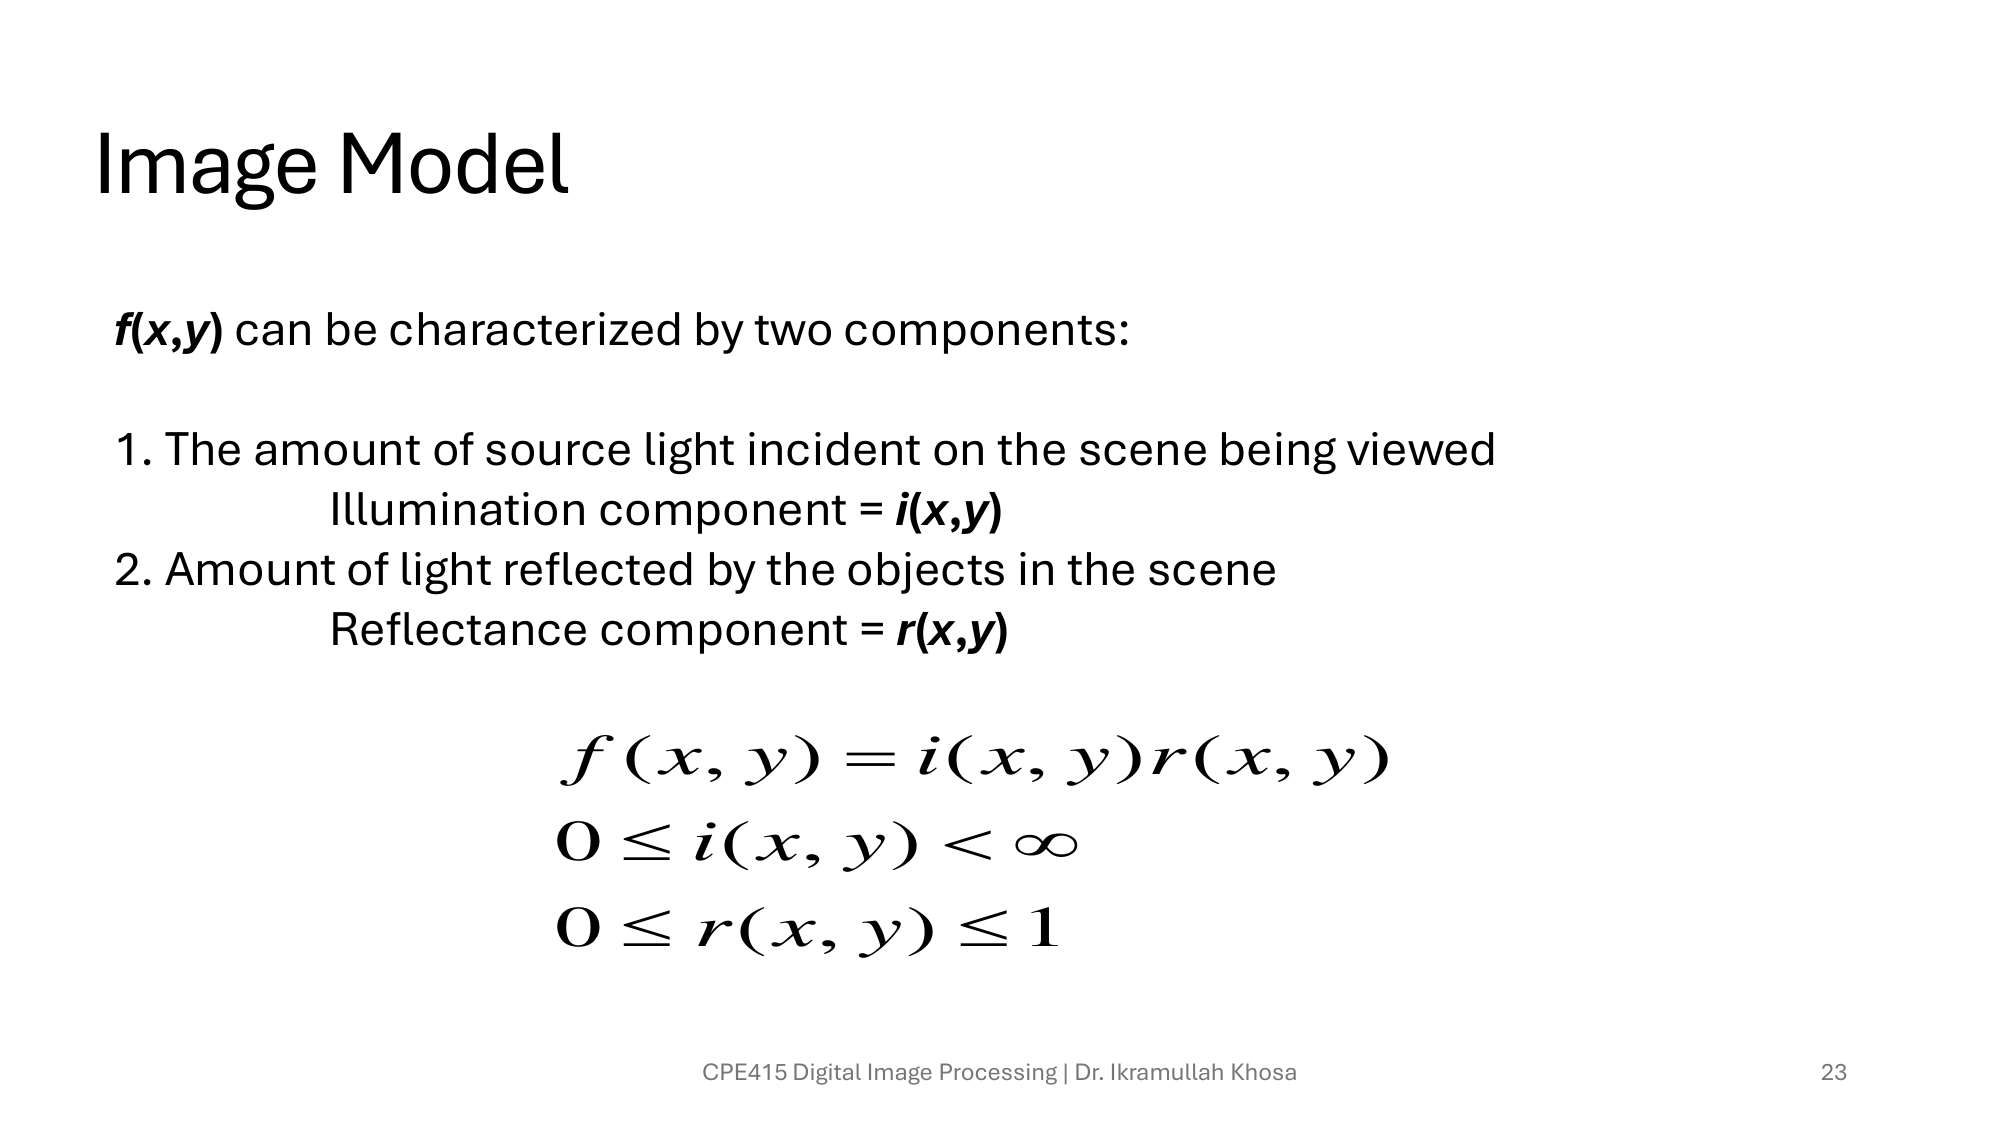
\includegraphics[width=0.9\textwidth]{images/slide2-23.png}
    \caption{Sampling and quantization process}
    \label{fig:sampling_quantization}
\end{figure}

\begin{deepexplanation}
\textbf{DEEP ANALYSIS - Figure \ref{fig:sampling_quantization}: The Two-Step Digitization}

\textbf{Step 1: Sampling (Spatial Discretization)}
\begin{itemize}
    \item Continuous: $f(x, y)$ defined for all real $(x, y)$ in some domain
    \item Sampled: $f(m\Delta x, n\Delta y)$ for integers $m, n$
    \item $\Delta x, \Delta y$ = sampling intervals (pixel spacing)
    \item Result: $M \times N$ grid of samples
\end{itemize}

\textbf{Step 2: Quantization (Intensity Discretization)}
\begin{itemize}
    \item Continuous: Intensity can be any real value in $[0, L_{max}]$
    \item Quantized: Intensity mapped to one of $L$ discrete levels
    \item Typically $L = 2^k$ (k bits): $L = 256$ for 8-bit
    \item Quantization interval: $\Delta q = L_{max} / L$
\end{itemize}

\textbf{Mathematical Representation:}
\begin{itemize}
    \item Sampling: Multiplication by 2D impulse train
    \[
    f_s(x,y) = f(x,y) \cdot \sum_{m=-\infty}^{\infty} \sum_{n=-\infty}^{\infty} \delta(x - m\Delta x, y - n\Delta y)
    \]
    \item Quantization: Rounding function
    \[
    f_q = \Delta q \cdot \text{round}\left(\frac{f}{\Delta q}\right)
    \]
\end{itemize}

\textbf{Errors Introduced:}
\begin{itemize}
    \item \textbf{Sampling}: Aliasing (if sampling theorem violated)
    \item \textbf{Quantization}: Quantization noise (information loss)
\end{itemize}
\end{deepexplanation}

\subsection{Sampling and the Nyquist Theorem}

\begin{figure}[H]
    \centering
    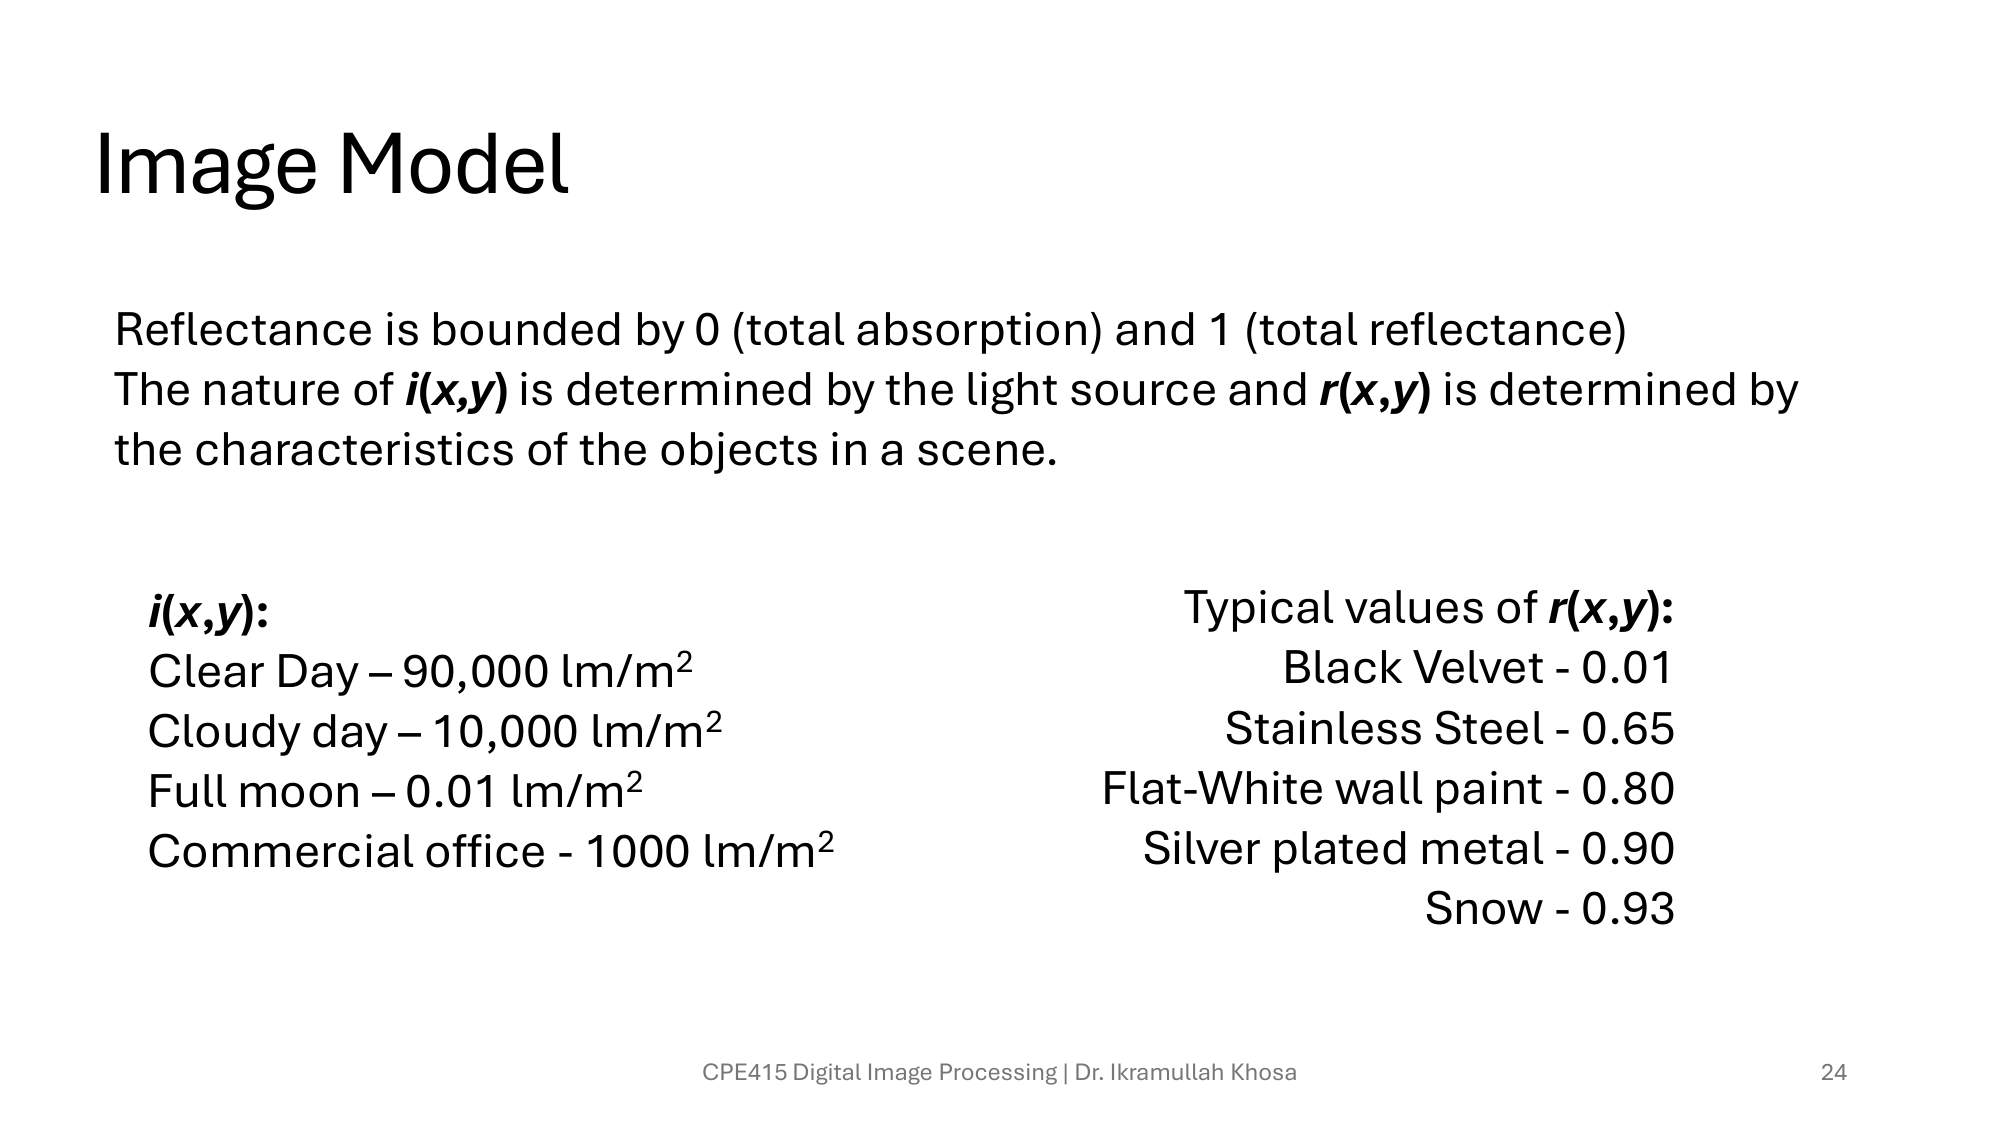
\includegraphics[width=0.85\textwidth]{images/slide2-24.png}
    \caption{1D sampling illustration}
    \label{fig:1d_sampling}
\end{figure}

\begin{deepexplanation}
\textbf{DEEP ANALYSIS - Figure \ref{fig:1d_sampling}: Understanding Sampling in 1D}

\textbf{The Sampling Process Visualized:}
\begin{enumerate}
    \item Start with continuous signal $f(x)$
    \item Sample at regular intervals $\Delta x$
    \item Obtain discrete sequence $f[n] = f(n \cdot \Delta x)$
\end{enumerate}

\textbf{The Nyquist-Shannon Sampling Theorem:}

\begin{importantbox}
A bandlimited signal with maximum frequency $f_{max}$ can be \textbf{perfectly reconstructed} from its samples if:
\[
f_s \geq 2 f_{max}
\]
where $f_s = 1/\Delta x$ is the sampling frequency.

$f_N = f_s/2 = 1/(2\Delta x)$ is called the \textbf{Nyquist frequency}.
\end{importantbox}

\textbf{What Happens in Frequency Domain:}
Sampling causes the spectrum to be \textbf{replicated} at multiples of $f_s$:
\[
F_s(u) = \frac{1}{\Delta x} \sum_{k=-\infty}^{\infty} F(u - k \cdot f_s)
\]

If $f_{max} < f_s/2$: Replicas don't overlap $\rightarrow$ can recover original.

If $f_{max} > f_s/2$: Replicas overlap $\rightarrow$ \textbf{aliasing} $\rightarrow$ information lost!

\textbf{For Images (2D):}
Need to satisfy Nyquist in \textbf{both} $x$ and $y$ directions:
\[
f_{s,x} \geq 2 f_{max,x} \quad \text{and} \quad f_{s,y} \geq 2 f_{max,y}
\]
\end{deepexplanation}

\begin{figure}[H]
    \centering
    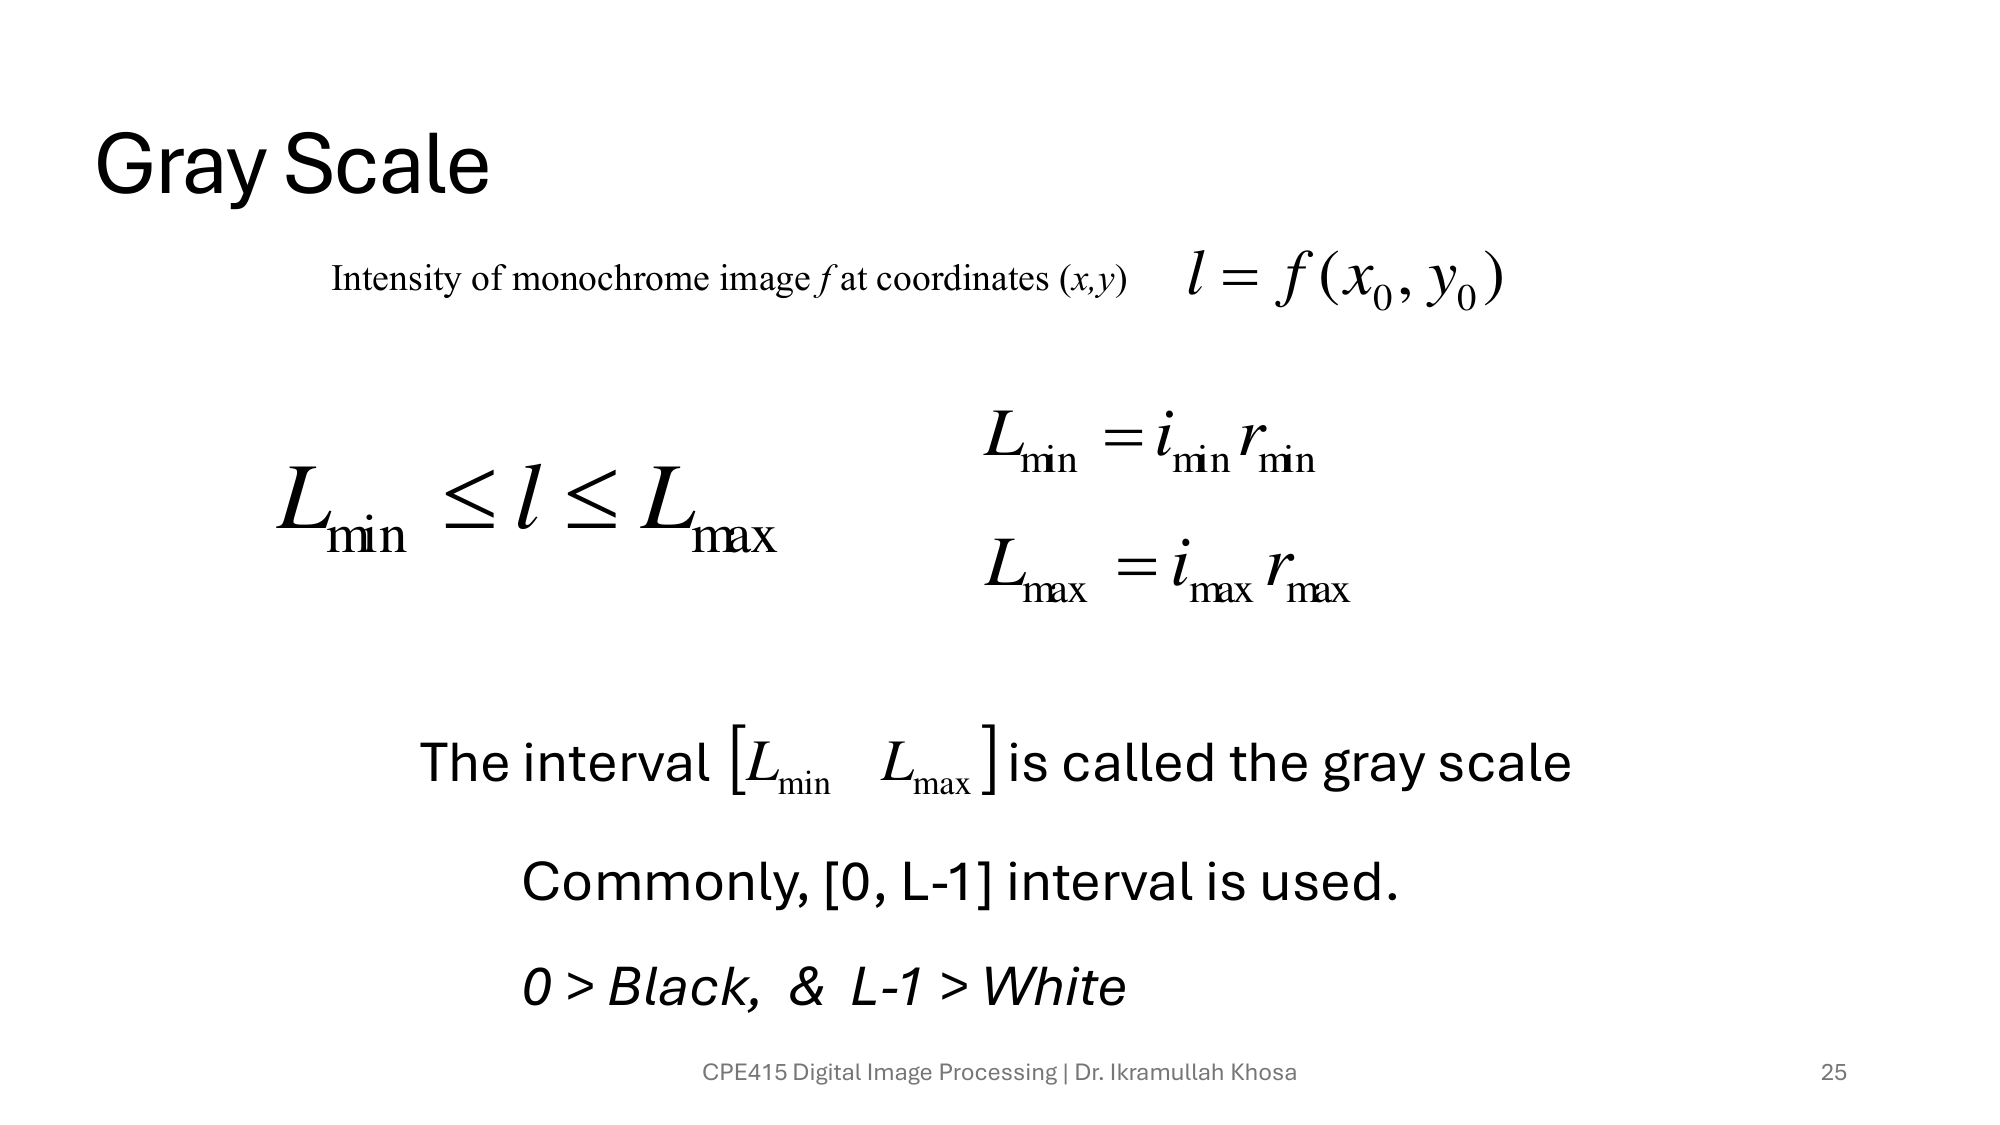
\includegraphics[width=0.85\textwidth]{images/slide2-25.png}
    \caption{Aliasing artifacts due to undersampling}
    \label{fig:aliasing}
\end{figure}

\begin{deepexplanation}
\textbf{DEEP ANALYSIS - Figure \ref{fig:aliasing}: The Aliasing Phenomenon}

\textbf{What Is Aliasing?}
When high-frequency components ``masquerade'' as lower frequencies due to insufficient sampling.

\textbf{Mathematical Cause:}
\begin{itemize}
    \item Signal contains frequency $f_{signal} > f_s/2$
    \item After sampling, this appears as frequency:
    \[
    f_{alias} = |f_{signal} - k \cdot f_s|
    \]
    where $k$ is chosen so $f_{alias} < f_s/2$
\end{itemize}

\textbf{Visual Examples:}

\textbf{1. Wagon Wheel Effect (Temporal Aliasing):}
\begin{itemize}
    \item Wheel spins at 30 rotations/second
    \item Video records at 24 frames/second
    \item Nyquist: Need $> 60$ fps to capture correctly
    \item Wheel appears to spin \textbf{backwards} at 6 rotations/second!
    \item $f_{alias} = |30 - 24| = 6$
\end{itemize}

\textbf{2. Moiré Patterns (Spatial Aliasing):}
\begin{itemize}
    \item Fabric with fine stripes (high spatial frequency)
    \item Sampled by camera sensor
    \item Creates wavy patterns that don't exist in original
\end{itemize}

\textbf{3. Jagged Edges (``Jaggies''):}
\begin{itemize}
    \item Diagonal lines in digital images
    \item Step-like appearance due to pixel grid
    \item Spatial aliasing of high-frequency edge
\end{itemize}

\textbf{How to Prevent Aliasing:}
\begin{enumerate}
    \item \textbf{Increase sampling rate}: Use higher resolution
    \item \textbf{Anti-aliasing filter}: Low-pass filter \textbf{before} sampling to remove frequencies $> f_s/2$
    \item \textbf{Optical low-pass filter}: Blur lens (common in cameras)
\end{enumerate}
\end{deepexplanation}

\begin{figure}[H]
    \centering
    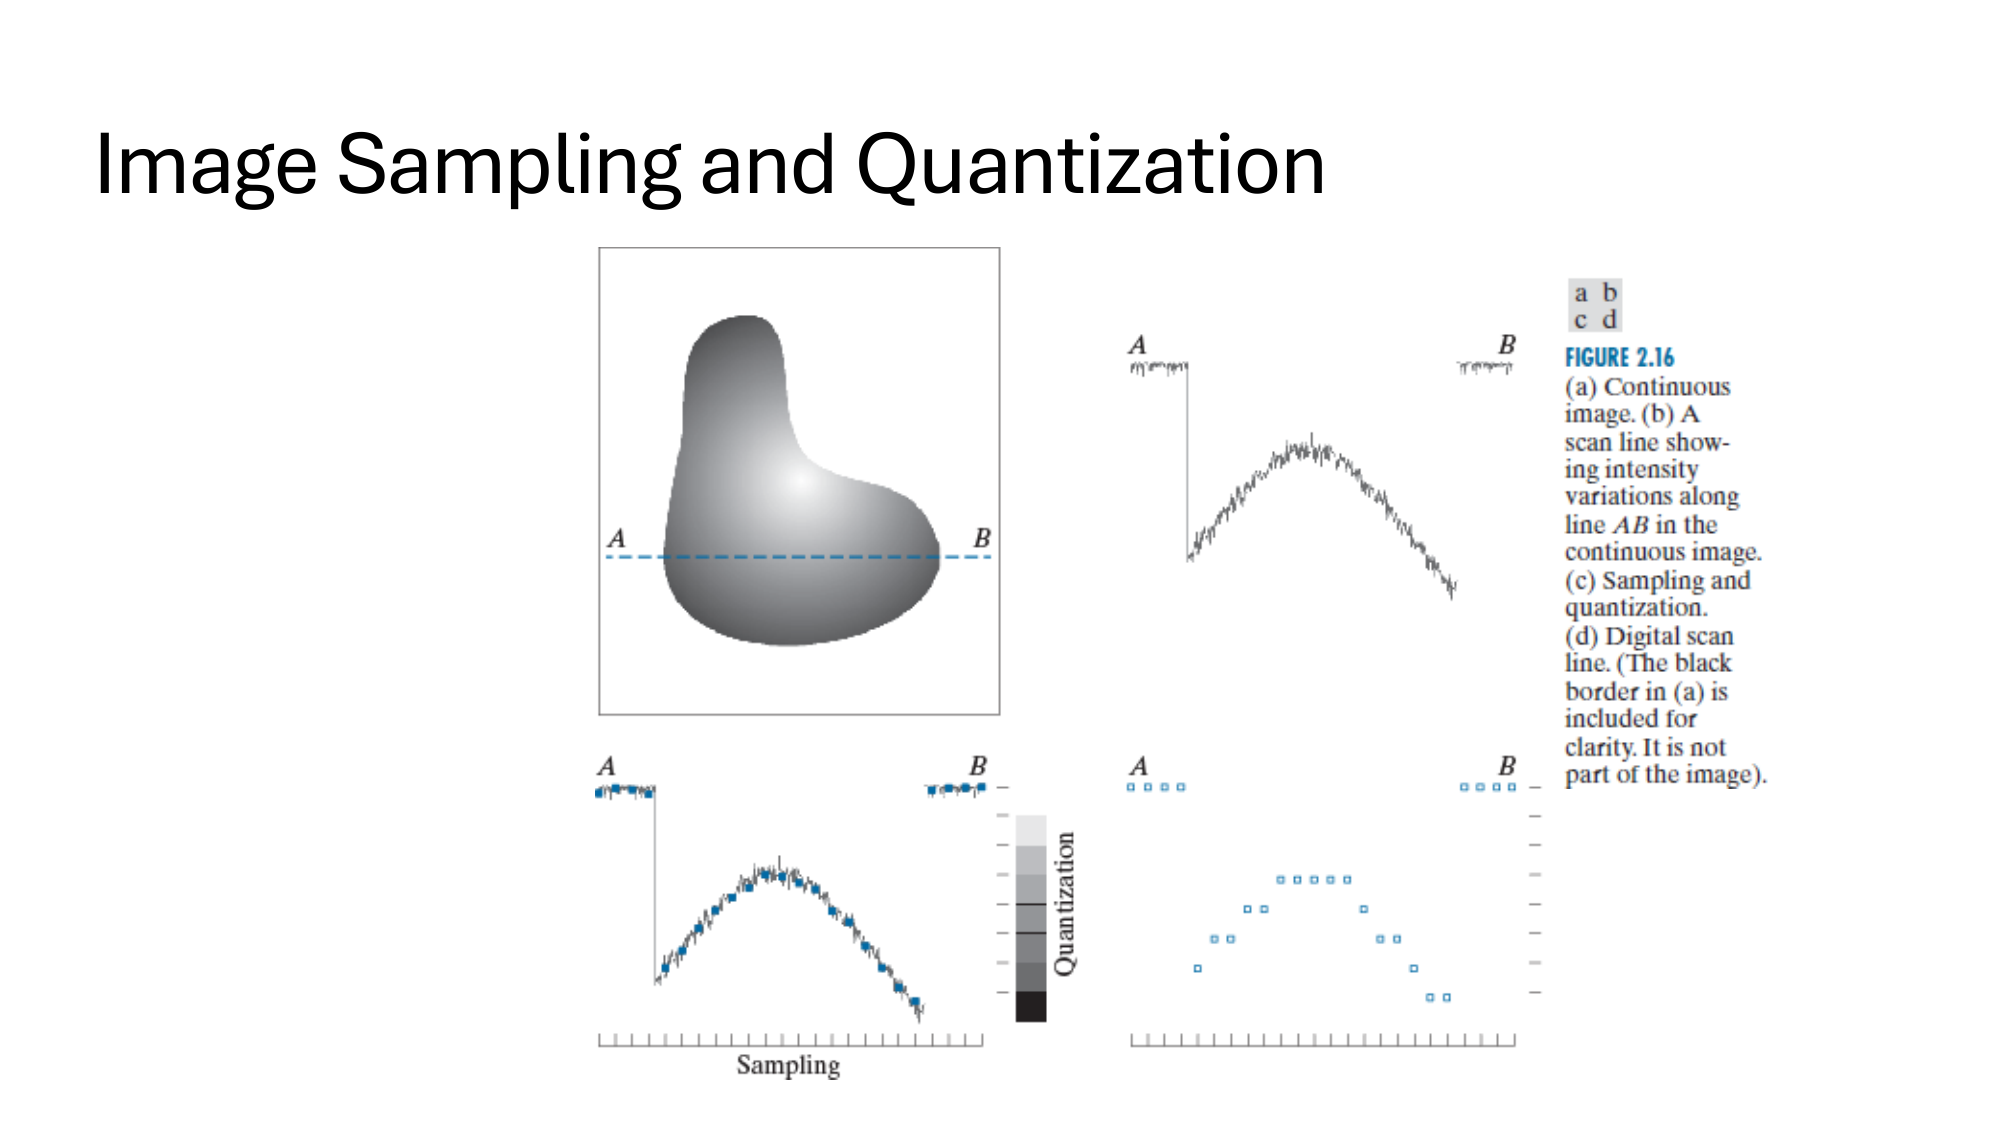
\includegraphics[width=0.85\textwidth]{images/slide2-26.png}
    \caption{Quantization levels and gray scale representation}
    \label{fig:quantization_levels}
\end{figure}

\begin{deepexplanation}
\textbf{DEEP ANALYSIS - Figure \ref{fig:quantization_levels}: Intensity Quantization}

\textbf{The Quantization Function:}
Map continuous intensity range $[0, L_{max}]$ to $L$ discrete levels:
\[
q(f) = \text{round}\left(\frac{f \cdot (L-1)}{L_{max}}\right)
\]

\textbf{Quantization Error:}
\begin{itemize}
    \item Maximum error: $\pm \Delta q/2$ where $\Delta q = L_{max}/L$
    \item Uniform quantization: All intervals equal
    \item Non-uniform quantization: Smaller intervals where precision needed more
\end{itemize}

\textbf{How Many Bits Are Enough?}

\textbf{Perceptual Argument:}
\begin{itemize}
    \item Weber's Law: JND $\approx 1$--$2\%$ of intensity
    \item 256 levels (8 bits): Steps $\approx 0.4\%$ --- smaller than JND
    \item 128 levels (7 bits): Steps $\approx 0.8\%$ --- still acceptable
    \item 64 levels (6 bits): Steps $\approx 1.6\%$ --- visible banding in smooth gradients
\end{itemize}

\textbf{Quantization Noise:}
\begin{itemize}
    \item Treat quantization error as additive noise
    \item For uniform quantization over $[0, 1]$ with $L$ levels:
    \[
    \sigma_q^2 = \frac{1}{12L^2} \quad \text{(variance)}
    \]
    \item Signal-to-Quantization-Noise Ratio (SQNR):
    \[
    \text{SQNR} \approx 6.02 \cdot k \text{ dB} \quad \text{for } k \text{ bits}
    \]
    8 bits $\rightarrow$ SQNR $\approx 48$ dB
\end{itemize}

\textbf{False Contouring:}
When quantization is too coarse, smooth gradients show visible ``steps'' --- especially noticeable due to Mach band effect.
\end{deepexplanation}

\begin{figure}[H]
    \centering
    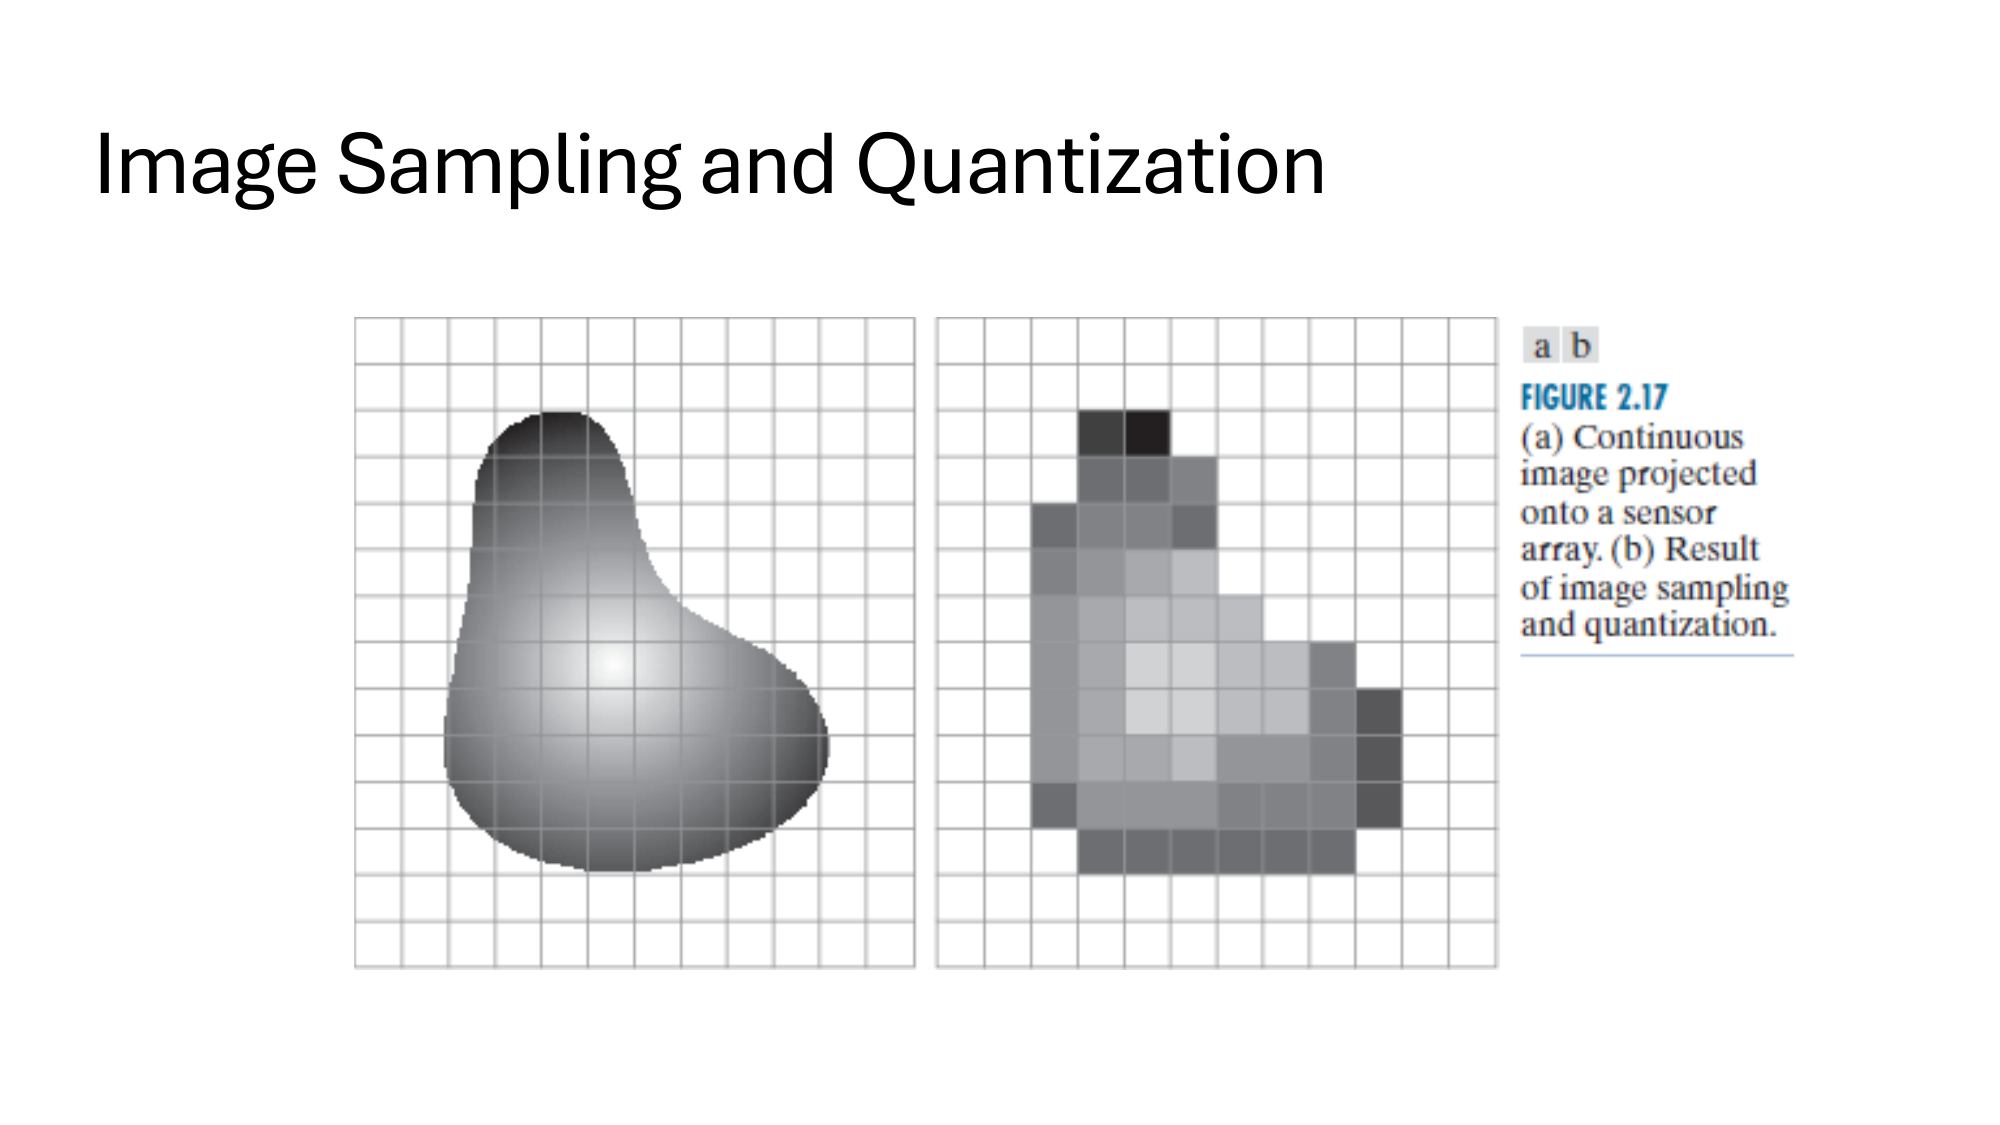
\includegraphics[width=0.85\textwidth]{images/slide2-27.png}
    \caption{Effect of different quantization levels on image quality}
    \label{fig:quantization_effects}
\end{figure}

\begin{deepexplanation}
\textbf{DEEP ANALYSIS - Figure \ref{fig:quantization_effects}: Visual Impact of Bit Depth}

\textbf{What the Figure Shows:}
Same image quantized to different numbers of gray levels, demonstrating quality degradation.

\textbf{Expected Observations:}
\begin{center}
\begin{tabular}{|c|c|l|}
\hline
\textbf{Bits} & \textbf{Levels} & \textbf{Quality} \\
\hline
8 & 256 & Excellent --- indistinguishable from original \\
7 & 128 & Very good --- minor banding possible \\
6 & 64 & Good --- slight banding in gradients \\
5 & 32 & Acceptable --- visible banding \\
4 & 16 & Poor --- obvious contouring \\
3 & 8 & Bad --- severe posterization \\
2 & 4 & Very bad --- nearly cartoon-like \\
1 & 2 & Binary --- only black and white \\
\hline
\end{tabular}
\end{center}

\textbf{Why Smooth Regions Show Artifacts First:}
\begin{itemize}
    \item Smooth gradients span many quantization levels
    \item Each ``jump'' between levels creates a visible edge (false contour)
    \item Mach bands amplify these false contours
    \item High-detail regions mask quantization artifacts
\end{itemize}

\textbf{Dithering Solution:}
Add small random noise before quantization:
\begin{itemize}
    \item Breaks up false contours
    \item Trade spatial resolution for tonal resolution
    \item Used extensively in printing (halftoning)
\end{itemize}
\end{deepexplanation}

%==============================================================================
\section{Digital Image Representation}
%==============================================================================

\subsection{Image as a Matrix}

\begin{figure}[H]
    \centering
    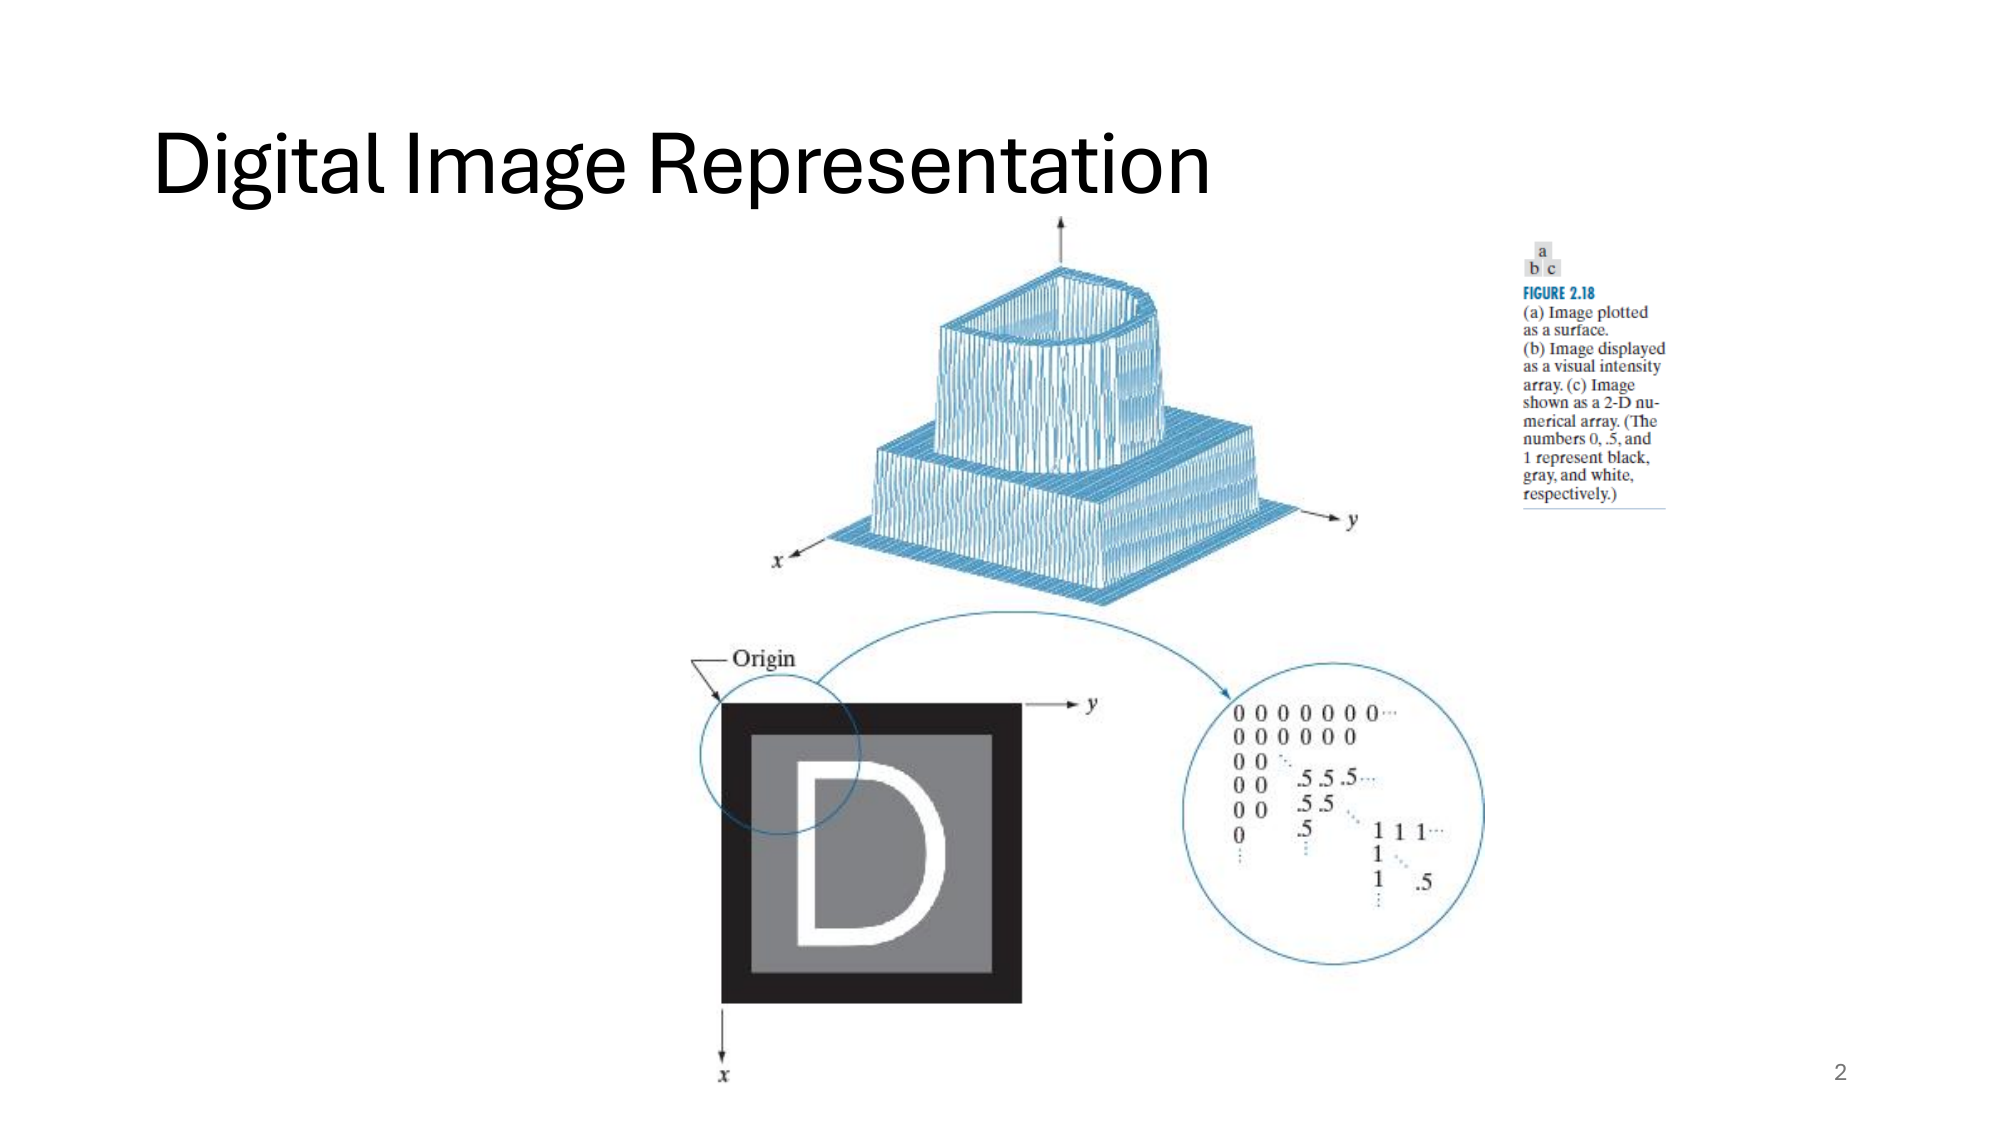
\includegraphics[width=0.9\textwidth]{images/slide3-02.png}
    \caption{Digital image as a 2D array of pixels}
    \label{fig:image_matrix}
\end{figure}

\begin{deepexplanation}
\textbf{DEEP ANALYSIS - Figure \ref{fig:image_matrix}: The Matrix Representation}

\textbf{Mathematical Notation:}
An $M \times N$ image with $L$ gray levels:
\[
f(x,y) = \begin{bmatrix}
f(0,0) & f(0,1) & \cdots & f(0,N-1) \\
f(1,0) & f(1,1) & \cdots & f(1,N-1) \\
\vdots & \vdots & \ddots & \vdots \\
f(M-1,0) & f(M-1,1) & \cdots & f(M-1,N-1)
\end{bmatrix}
\]

\textbf{Coordinate Convention (Important!):}
\begin{itemize}
    \item Origin $(0,0)$ at \textbf{top-left} (image processing convention)
    \item $x$ increases \textbf{downward} (row index)
    \item $y$ increases \textbf{rightward} (column index)
    \item Different from mathematical $(x,y)$ convention!
\end{itemize}

\textbf{Index Ranges:}
\begin{itemize}
    \item Rows: $x \in \{0, 1, 2, \ldots, M-1\}$
    \item Columns: $y \in \{0, 1, 2, \ldots, N-1\}$
    \item Intensity: $f(x,y) \in \{0, 1, 2, \ldots, L-1\}$
\end{itemize}

\textbf{Typical Values:}
\begin{itemize}
    \item For $k$-bit image: $L = 2^k$ (e.g., 256 for 8-bit)
    \item Often $M = N = 2^n$ (power of 2) for FFT efficiency
    \item Common sizes: $256 \times 256$, $512 \times 512$, $1024 \times 1024$
\end{itemize}

\textbf{Memory Layout:}
\begin{itemize}
    \item Row-major order: Rows stored contiguously (C, Python)
    \item Column-major order: Columns stored contiguously (MATLAB, Fortran)
    \item This affects memory access efficiency!
\end{itemize}
\end{deepexplanation}

\subsection{Storage Requirements}

\begin{figure}[H]
    \centering
    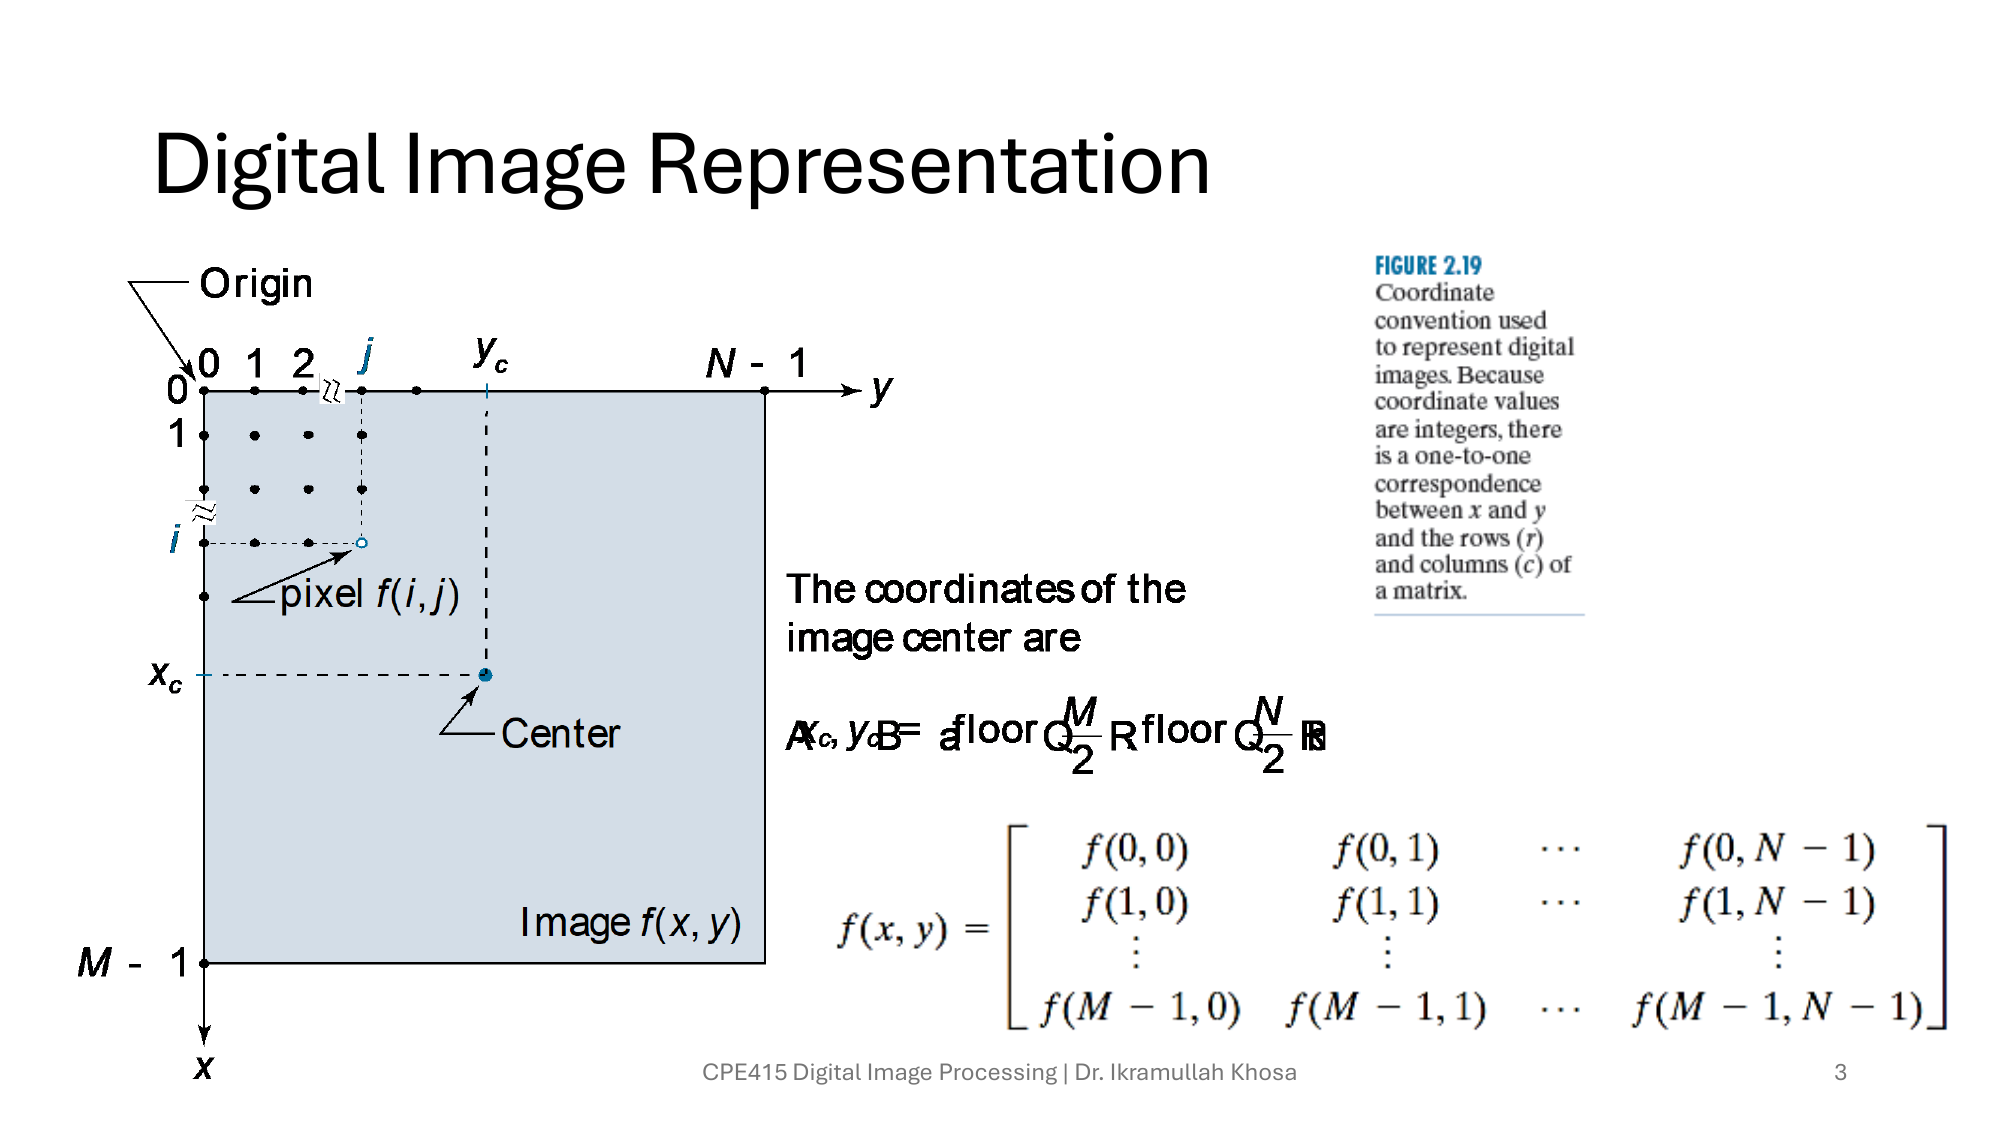
\includegraphics[width=0.85\textwidth]{images/slide3-03.png}
    \caption{Image storage requirements calculation}
    \label{fig:storage}
\end{figure}

\begin{deepexplanation}
\textbf{DEEP ANALYSIS - Figure \ref{fig:storage}: Calculating Image Size}

\textbf{The Formula:}
\[
b = M \times N \times k \text{ bits}
\]
where $M \times N$ = number of pixels, $k$ = bits per pixel.

\textbf{Example Calculations:}
\begin{center}
\begin{tabular}{|l|c|c|c|}
\hline
\textbf{Image Size} & \textbf{Bits/Pixel} & \textbf{Total Bits} & \textbf{Bytes} \\
\hline
$256 \times 256$ & 8 & $524,288$ & 64 KB \\
$512 \times 512$ & 8 & $2,097,152$ & 256 KB \\
$1024 \times 1024$ & 8 & $8,388,608$ & 1 MB \\
$1920 \times 1080$ (HD) & 24 (RGB) & $49,766,400$ & 5.9 MB \\
$4096 \times 3072$ (12MP) & 24 (RGB) & $301,989,888$ & 36 MB \\
\hline
\end{tabular}
\end{center}

\textbf{Color Images:}
\begin{itemize}
    \item RGB: 3 channels $\times$ 8 bits = 24 bits/pixel (true color)
    \item RGBA: 4 channels $\times$ 8 bits = 32 bits/pixel (with alpha)
    \item High dynamic range: 16 or 32 bits/channel
\end{itemize}

\textbf{Why Compression Is Essential:}
\begin{itemize}
    \item 1 minute of uncompressed HD video (30 fps):
    \[
    1920 \times 1080 \times 3 \times 30 \times 60 = 11.2 \text{ GB}
    \]
    \item JPEG typically achieves 10:1 compression (lossy)
    \item PNG achieves 2:1 to 5:1 (lossless)
\end{itemize}
\end{deepexplanation}

\subsection{Dynamic Range}

\begin{figure}[H]
    \centering
    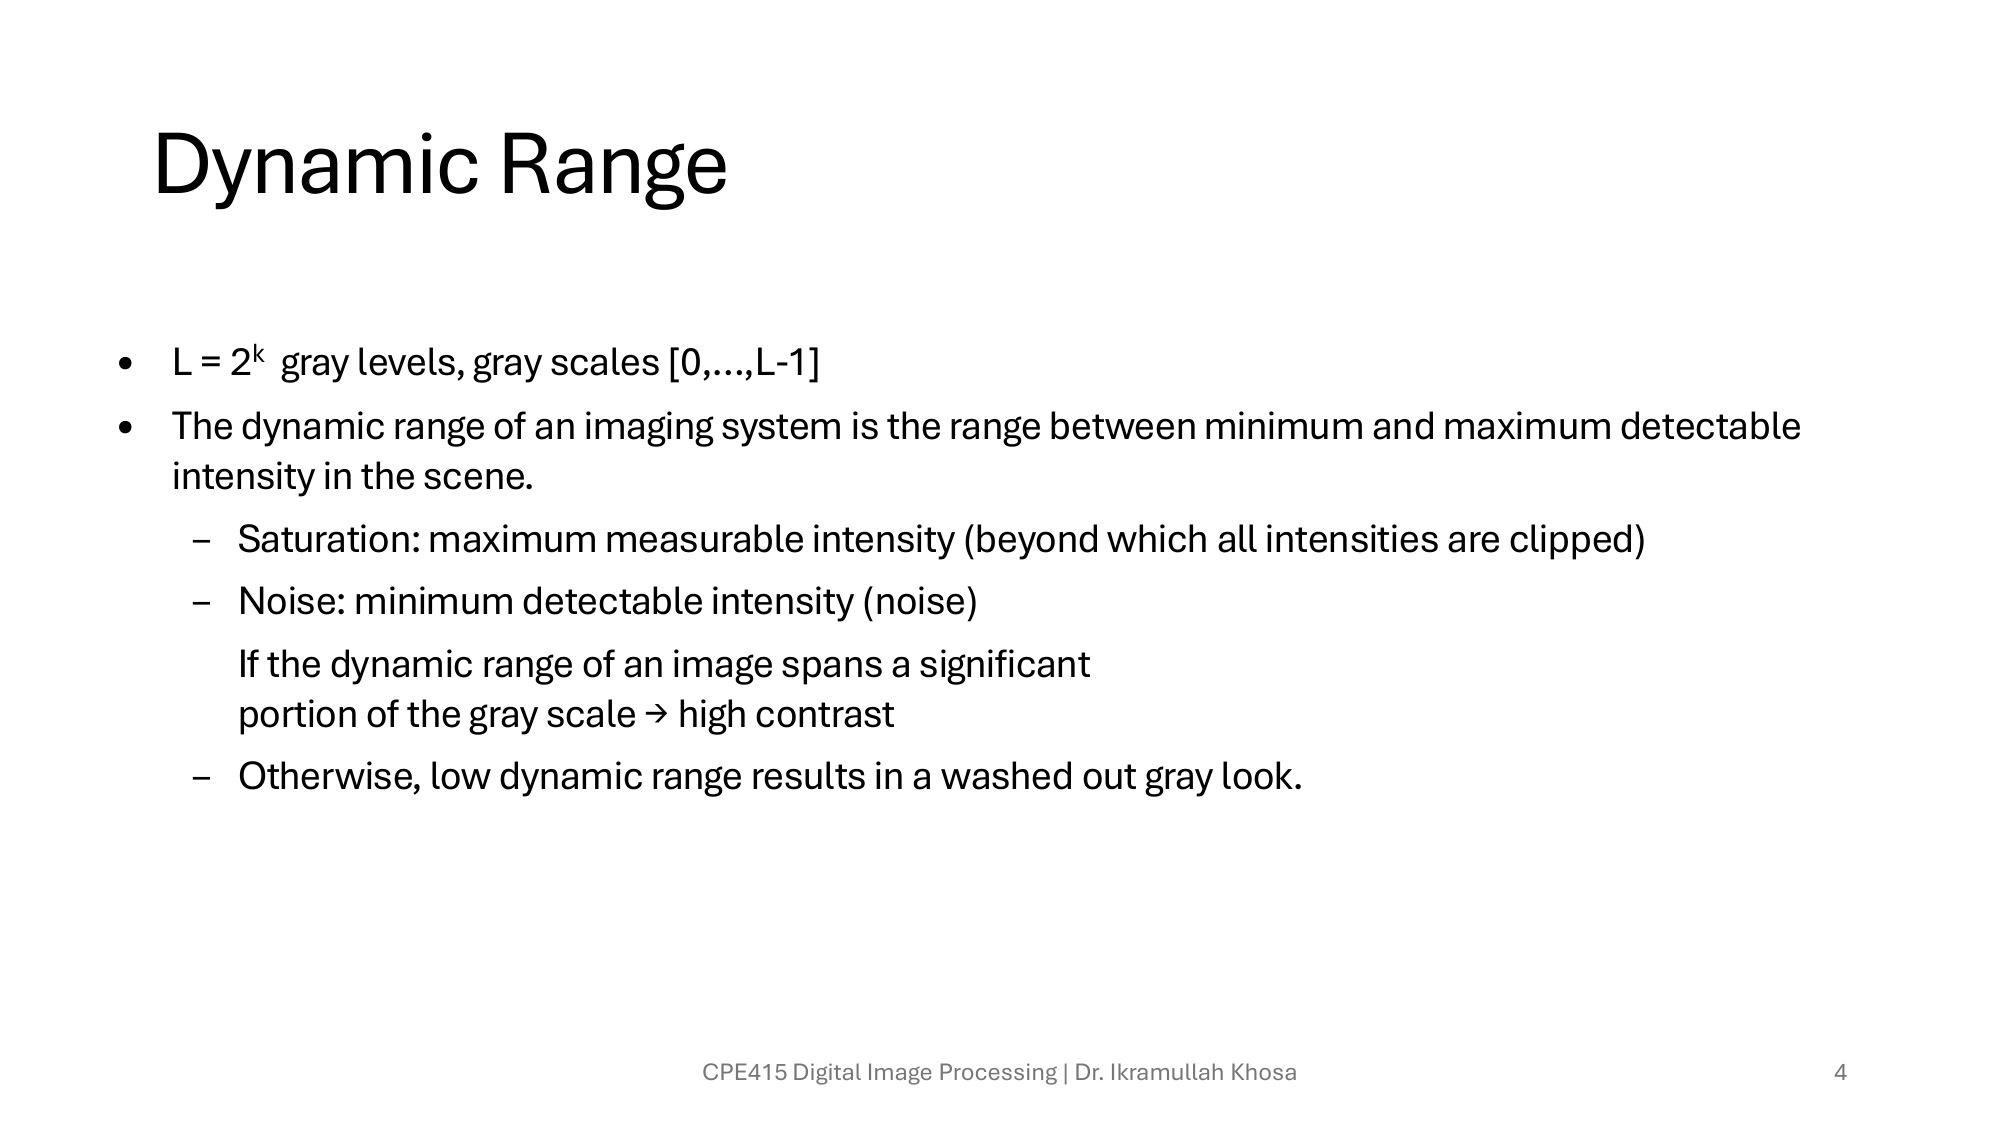
\includegraphics[width=0.85\textwidth]{images/slide3-04.png}
    \caption{Dynamic range and contrast in images}
    \label{fig:dynamic_range}
\end{figure}

\begin{deepexplanation}
\textbf{DEEP ANALYSIS - Figure \ref{fig:dynamic_range}: Understanding Dynamic Range}

\textbf{Definition:}
\[
\text{Dynamic Range} = \frac{I_{max}}{I_{min}}
\]
or in decibels:
\[
\text{DR (dB)} = 20 \log_{10}\left(\frac{I_{max}}{I_{min}}\right)
\]

\textbf{Contrast:}
\[
\text{Contrast} = \frac{I_{max} - I_{min}}{I_{max} + I_{min}}
\]
(Michelson contrast, ranges from 0 to 1)

\textbf{Comparison of Dynamic Ranges:}
\begin{center}
\begin{tabular}{|l|c|c|}
\hline
\textbf{Medium} & \textbf{DR Ratio} & \textbf{DR (dB)} \\
\hline
Human eye (adapted) & $10^{10}$ : 1 & 200 dB \\
Human eye (instantaneous) & 1000 : 1 & 60 dB \\
Real-world scene (sunny day) & 100,000 : 1 & 100 dB \\
Standard camera & 1000 : 1 & 60 dB \\
HDR camera & 100,000 : 1 & 100 dB \\
8-bit display & 256 : 1 & 48 dB \\
HDR display & 10,000 : 1 & 80 dB \\
Printed paper & 100 : 1 & 40 dB \\
\hline
\end{tabular}
\end{center}

\textbf{The HDR Problem:}
\begin{itemize}
    \item Real scenes have higher DR than displays can show
    \item Solution: Tone mapping --- compress HDR to displayable range
    \item Goal: Preserve \textbf{perceptual} appearance of contrast
\end{itemize}
\end{deepexplanation}


%==============================================================================
\section{Spatial and Intensity Resolution}
%==============================================================================

\subsection{Spatial Resolution}

\begin{conceptbox}[Resolution Definitions]
\textbf{Spatial Resolution}: The smallest discernible detail in an image.
\begin{itemize}
    \item Measured in: pixels per unit length (dpi, ppi), line pairs per mm (lp/mm)
    \item Higher resolution = finer detail captured
\end{itemize}

\textbf{Intensity (Gray-Level) Resolution}: The smallest discernible change in gray level.
\begin{itemize}
    \item Measured in: bits per pixel or number of gray levels
    \item Higher resolution = more shades distinguishable
\end{itemize}
\end{conceptbox}

\begin{figure}[H]
    \centering
    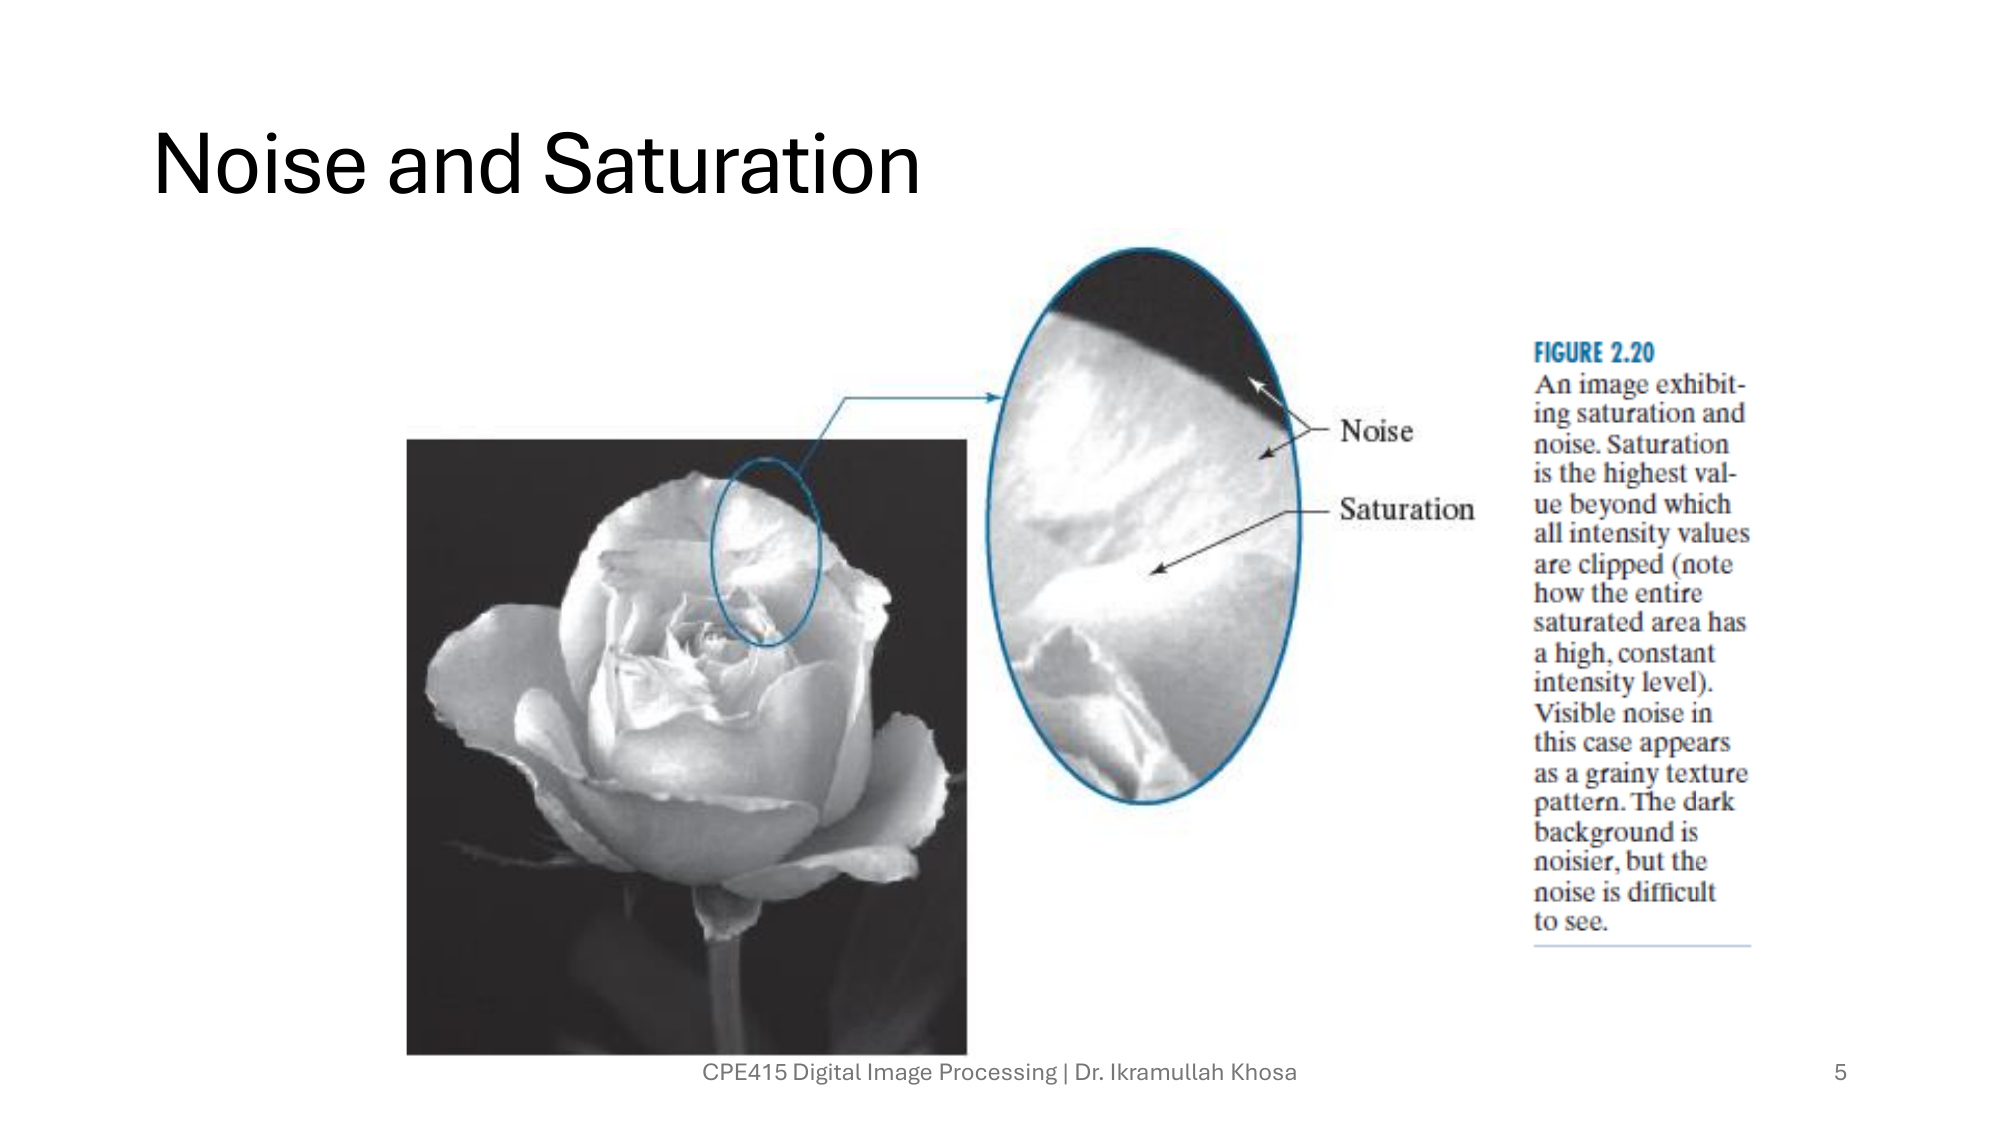
\includegraphics[width=0.9\textwidth]{images/slide3-05.png}
    \caption{Effect of reducing spatial resolution}
    \label{fig:spatial_resolution}
\end{figure}

\begin{deepexplanation}
\textbf{DEEP ANALYSIS - Figure \ref{fig:spatial_resolution}: Spatial Resolution Effects}

\textbf{What Happens When Resolution Decreases:}
\begin{enumerate}
    \item $1024 \times 1024$: Full detail visible --- hair strands, skin texture
    \item $512 \times 512$: Good quality --- most features preserved
    \item $256 \times 256$: Acceptable --- some fine detail lost
    \item $128 \times 128$: Degraded --- features become blocky
    \item $64 \times 64$: Poor --- face barely recognizable
    \item $32 \times 32$: Very poor --- major features as colored blocks
\end{enumerate}

\textbf{The Physics:}
When we reduce resolution by factor $k$:
\begin{itemize}
    \item Each new pixel averages $k \times k$ original pixels
    \item Effective sampling frequency reduced by $k$
    \item Frequencies above new Nyquist are lost (or aliased)
\end{itemize}

\textbf{Minimum Resolution for Recognition:}
\begin{itemize}
    \item Face recognition: $\approx 32 \times 32$ minimum
    \item License plate: $\approx 10$--$15$ pixels per character height
    \item General rule: Feature must span several pixels
\end{itemize}

\textbf{Resolution Units:}
\begin{center}
\begin{tabular}{|l|l|l|}
\hline
\textbf{Unit} & \textbf{Full Name} & \textbf{Typical Use} \\
\hline
dpi & dots per inch & Printing \\
ppi & pixels per inch & Displays, scanning \\
lp/mm & line pairs per mm & Optical systems \\
\hline
\end{tabular}
\end{center}

Conversion: $1 \text{ lp/mm} = 25.4 \text{ dpi} \times 2$ (need 2 pixels per line pair)
\end{deepexplanation}

\begin{figure}[H]
    \centering
    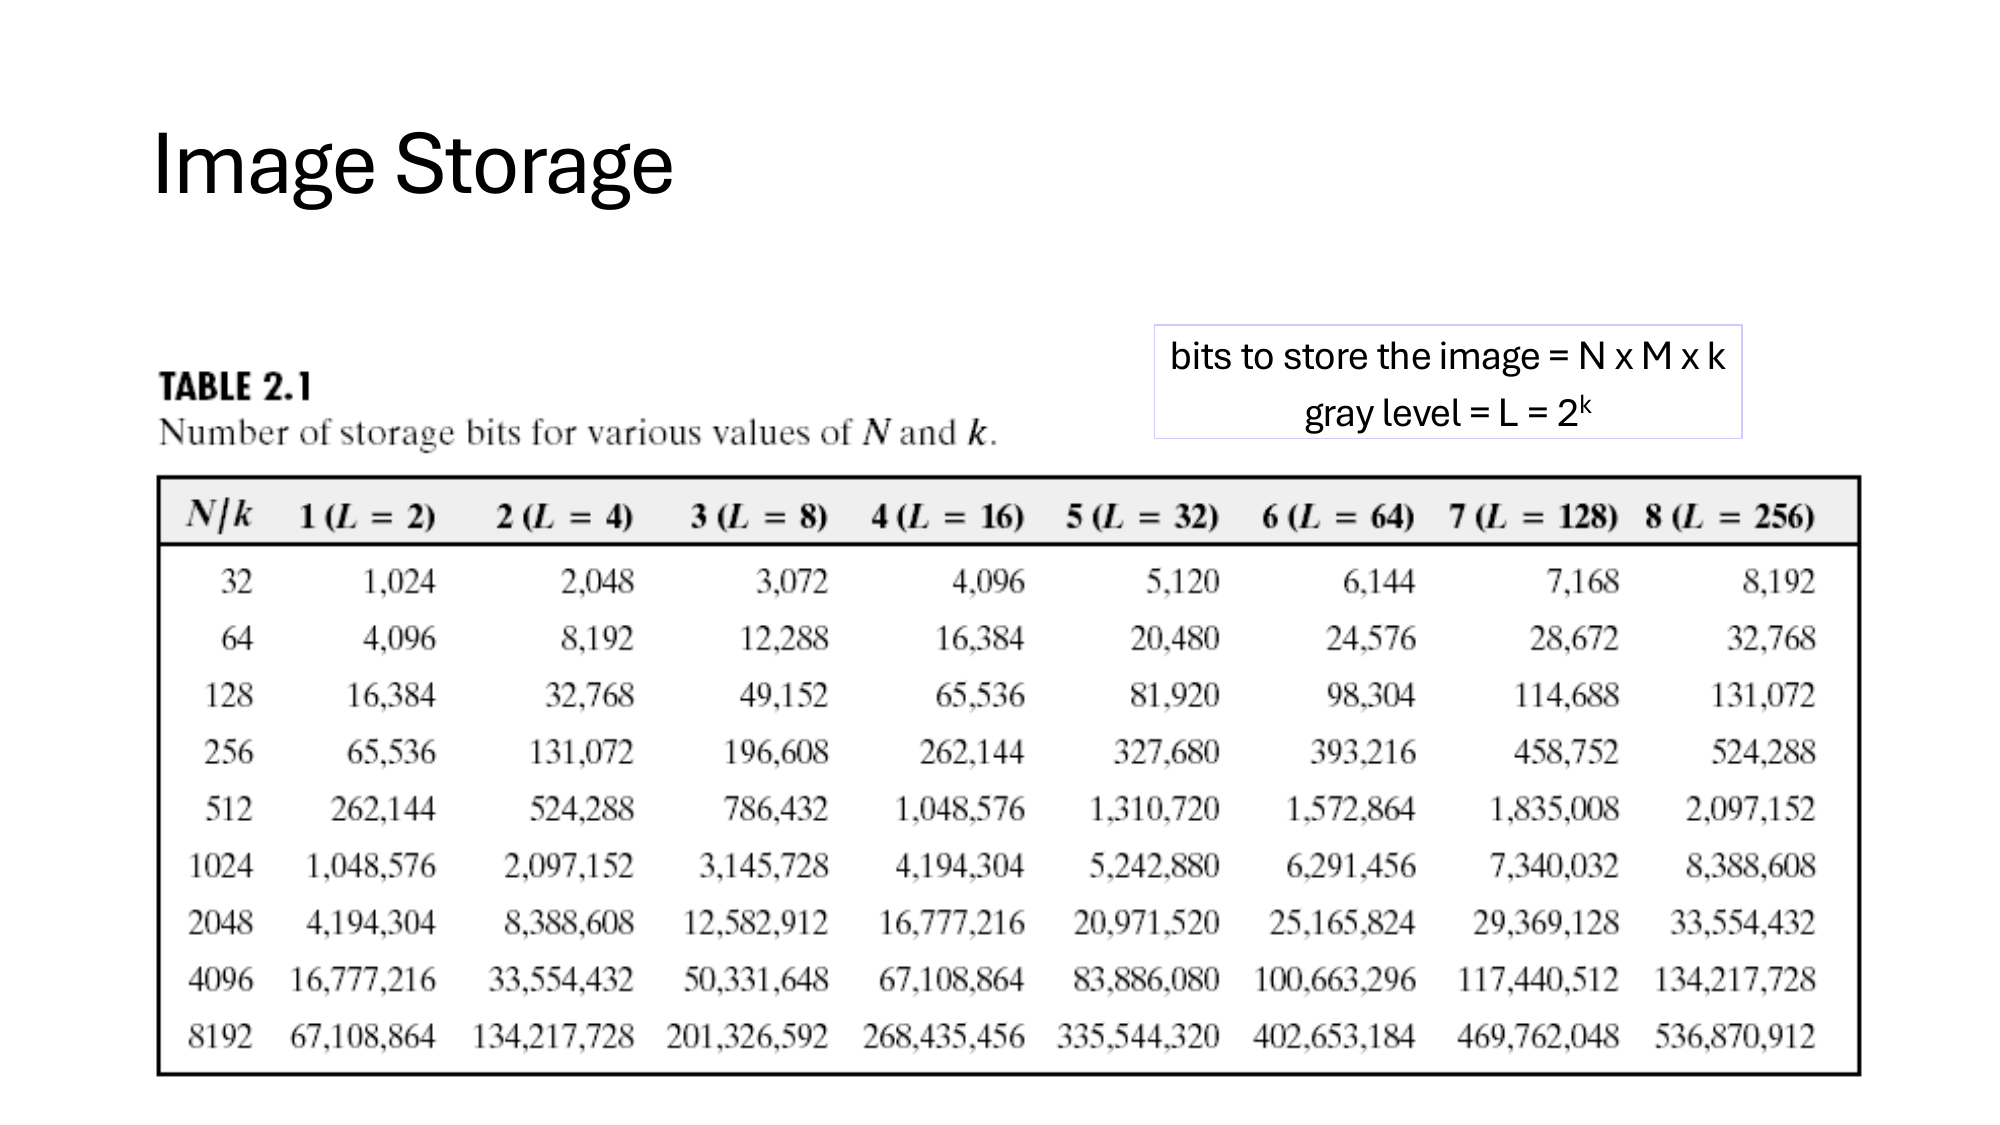
\includegraphics[width=0.85\textwidth]{images/slide3-06.png}
    \caption{Effect of reducing intensity (gray-level) resolution}
    \label{fig:intensity_resolution}
\end{figure}

\begin{deepexplanation}
\textbf{DEEP ANALYSIS - Figure \ref{fig:intensity_resolution}: Gray-Level Resolution Effects}

\textbf{What Happens When Bit Depth Decreases:}
\begin{enumerate}
    \item 8 bits (256 levels): Smooth gradients, photorealistic
    \item 7 bits (128 levels): Virtually identical to 8-bit
    \item 6 bits (64 levels): Minor banding in smooth areas
    \item 5 bits (32 levels): Noticeable false contours
    \item 4 bits (16 levels): Significant posterization
    \item 3 bits (8 levels): Severe banding, cartoon-like
    \item 2 bits (4 levels): Very coarse quantization
    \item 1 bit (2 levels): Binary --- black and white only
\end{enumerate}

\textbf{False Contouring Mechanism:}
\begin{itemize}
    \item Smooth gradient in original image
    \item Quantization creates ``steps'' at level boundaries
    \item Mach band effect amplifies perceived step edges
    \item Creates visible ``bands'' or ``contours''
\end{itemize}

\textbf{Which Images Are Most Affected?}
\begin{itemize}
    \item \textbf{Most sensitive}: Images with smooth gradients (sky, skin)
    \item \textbf{Least sensitive}: High-detail/textured images (foliage, fabric)
\end{itemize}

The texture masks the quantization artifacts!

\textbf{Practical Implications:}
\begin{itemize}
    \item 8 bits usually sufficient for photographic images
    \item Medical/scientific imaging may need 12--16 bits
    \item HDR imaging: 32-bit floating point common
\end{itemize}
\end{deepexplanation}

\subsection{Isopreference Curves}

\begin{figure}[H]
    \centering
    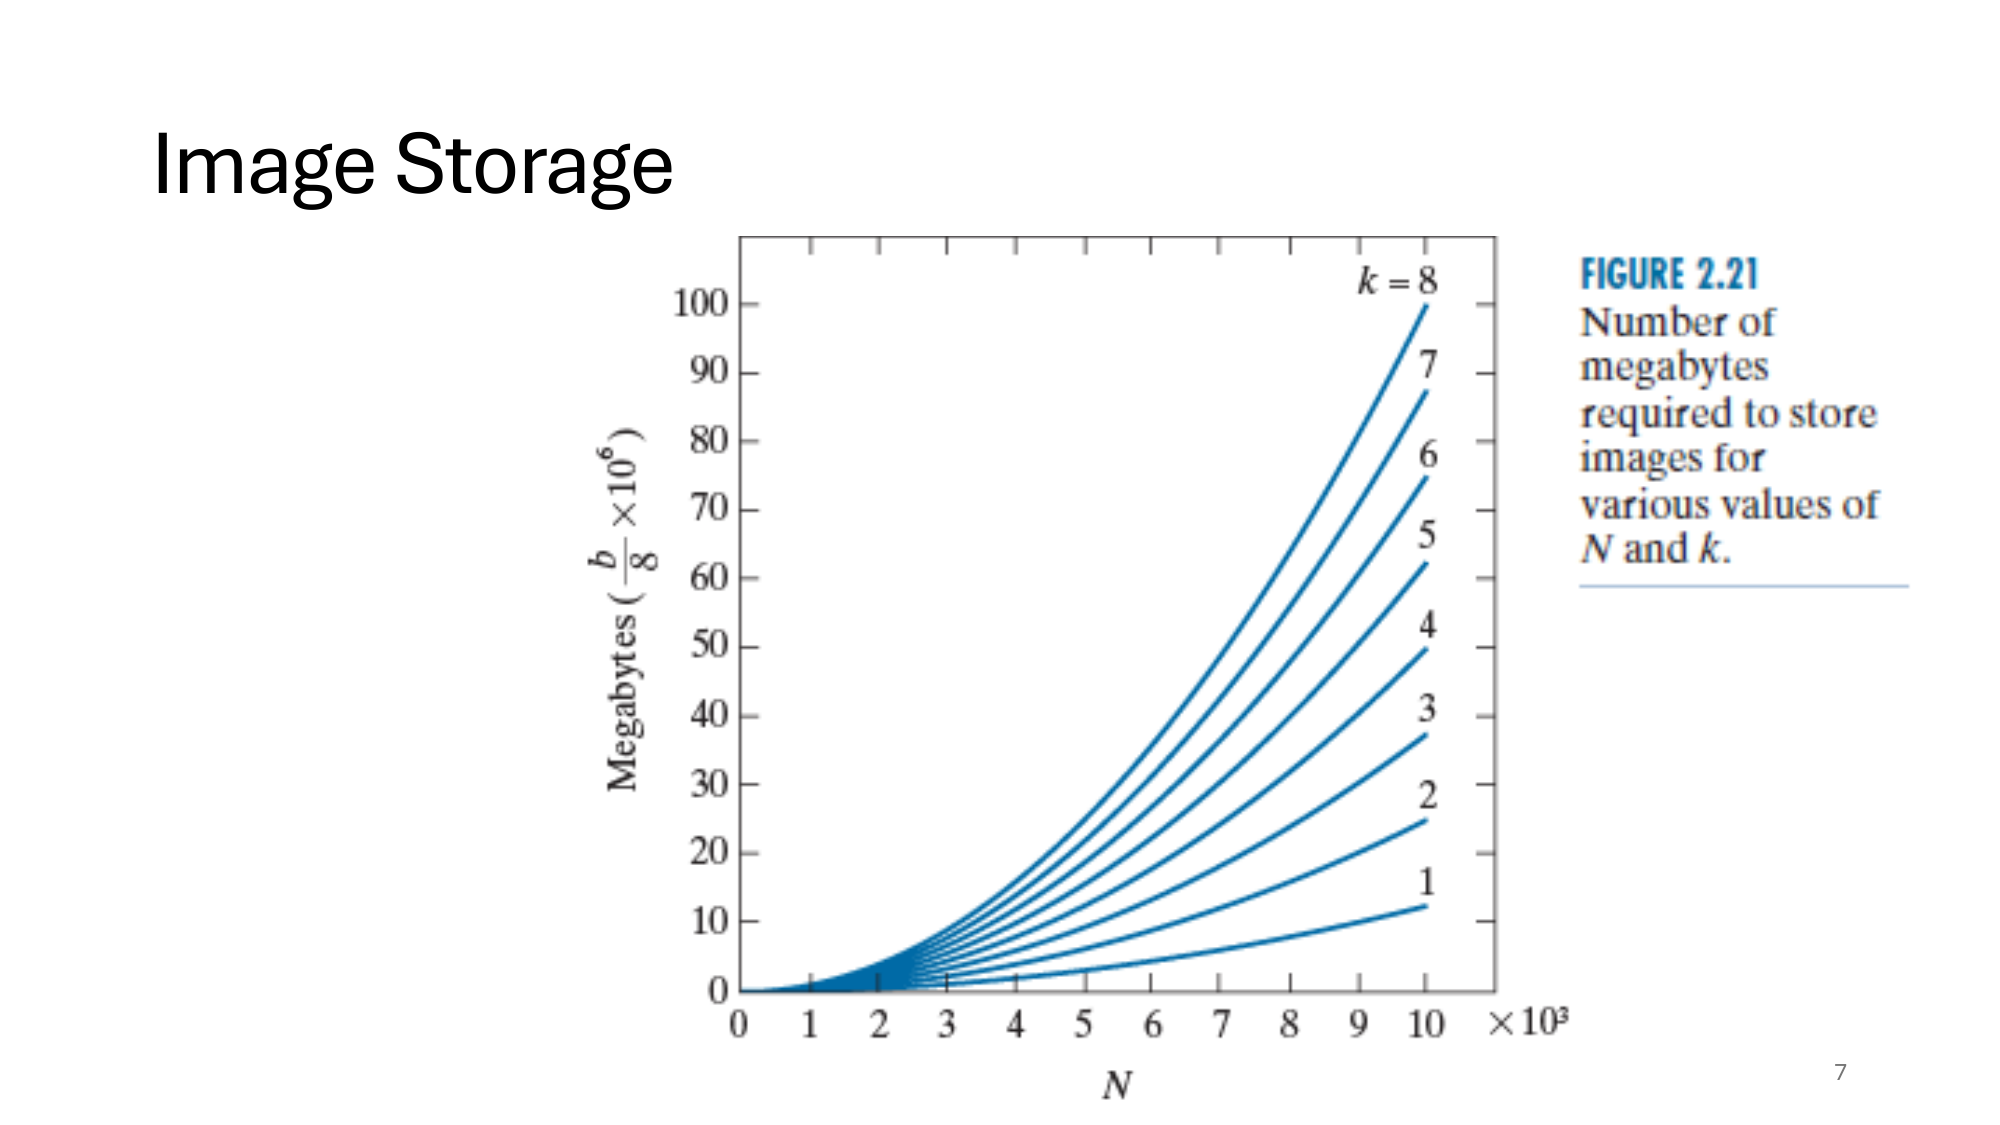
\includegraphics[width=0.85\textwidth]{images/slide3-07.png}
    \caption{Isopreference curves showing trade-off between spatial and intensity resolution}
    \label{fig:isopreference}
\end{figure}

\begin{deepexplanation}
\textbf{DEEP ANALYSIS - Figure \ref{fig:isopreference}: Resolution Trade-offs}

\textbf{What Isopreference Curves Show:}
Each curve connects combinations of (spatial resolution, gray-level resolution) that produce images of \textbf{equal subjective quality}.

\textbf{How They're Obtained:}
\begin{enumerate}
    \item Present subjects with images at various $(N, L)$ combinations
    \item Subject rates perceived quality
    \item Plot curves connecting equal-quality points
\end{enumerate}

\textbf{Key Observations:}

\textbf{1. Trade-off Exists:}
\begin{itemize}
    \item Can reduce gray levels if spatial resolution increases
    \item Can reduce spatial resolution if gray levels increase
    \item Total ``quality'' roughly constant along a curve
\end{itemize}

\textbf{2. Image Content Matters:}
\begin{itemize}
    \item High-detail images (crowds, foliage): Prefer spatial resolution
    \item Smooth images (portraits, sky): Prefer gray-level resolution
    \item Curves differ for different image types!
\end{itemize}

\textbf{3. Non-linear Trade-off:}
\begin{itemize}
    \item Not a simple $N \times L = \text{constant}$ relationship
    \item Below certain thresholds, quality drops rapidly
    \item Minimum practical: $\approx 4$--$5$ bits, $\approx 64 \times 64$ pixels
\end{itemize}

\textbf{Application:}
\begin{itemize}
    \item Compression: Allocate bits where they matter most
    \item Transmission: Adapt resolution to bandwidth/content
    \item Display: Match resolution to viewing distance
\end{itemize}
\end{deepexplanation}

%==============================================================================
\section{Image Interpolation}
%==============================================================================

\begin{conceptbox}[Why Interpolation?]
Interpolation is needed when:
\begin{itemize}
    \item \textbf{Zooming/scaling} an image
    \item \textbf{Rotating} an image (pixels don't align to grid)
    \item \textbf{Geometric correction} (removing lens distortion)
    \item \textbf{Image registration} (aligning images)
\end{itemize}
We need to estimate pixel values at \textbf{non-integer coordinates}.
\end{conceptbox}

\subsection{Nearest Neighbor Interpolation}

\begin{figure}[H]
    \centering
    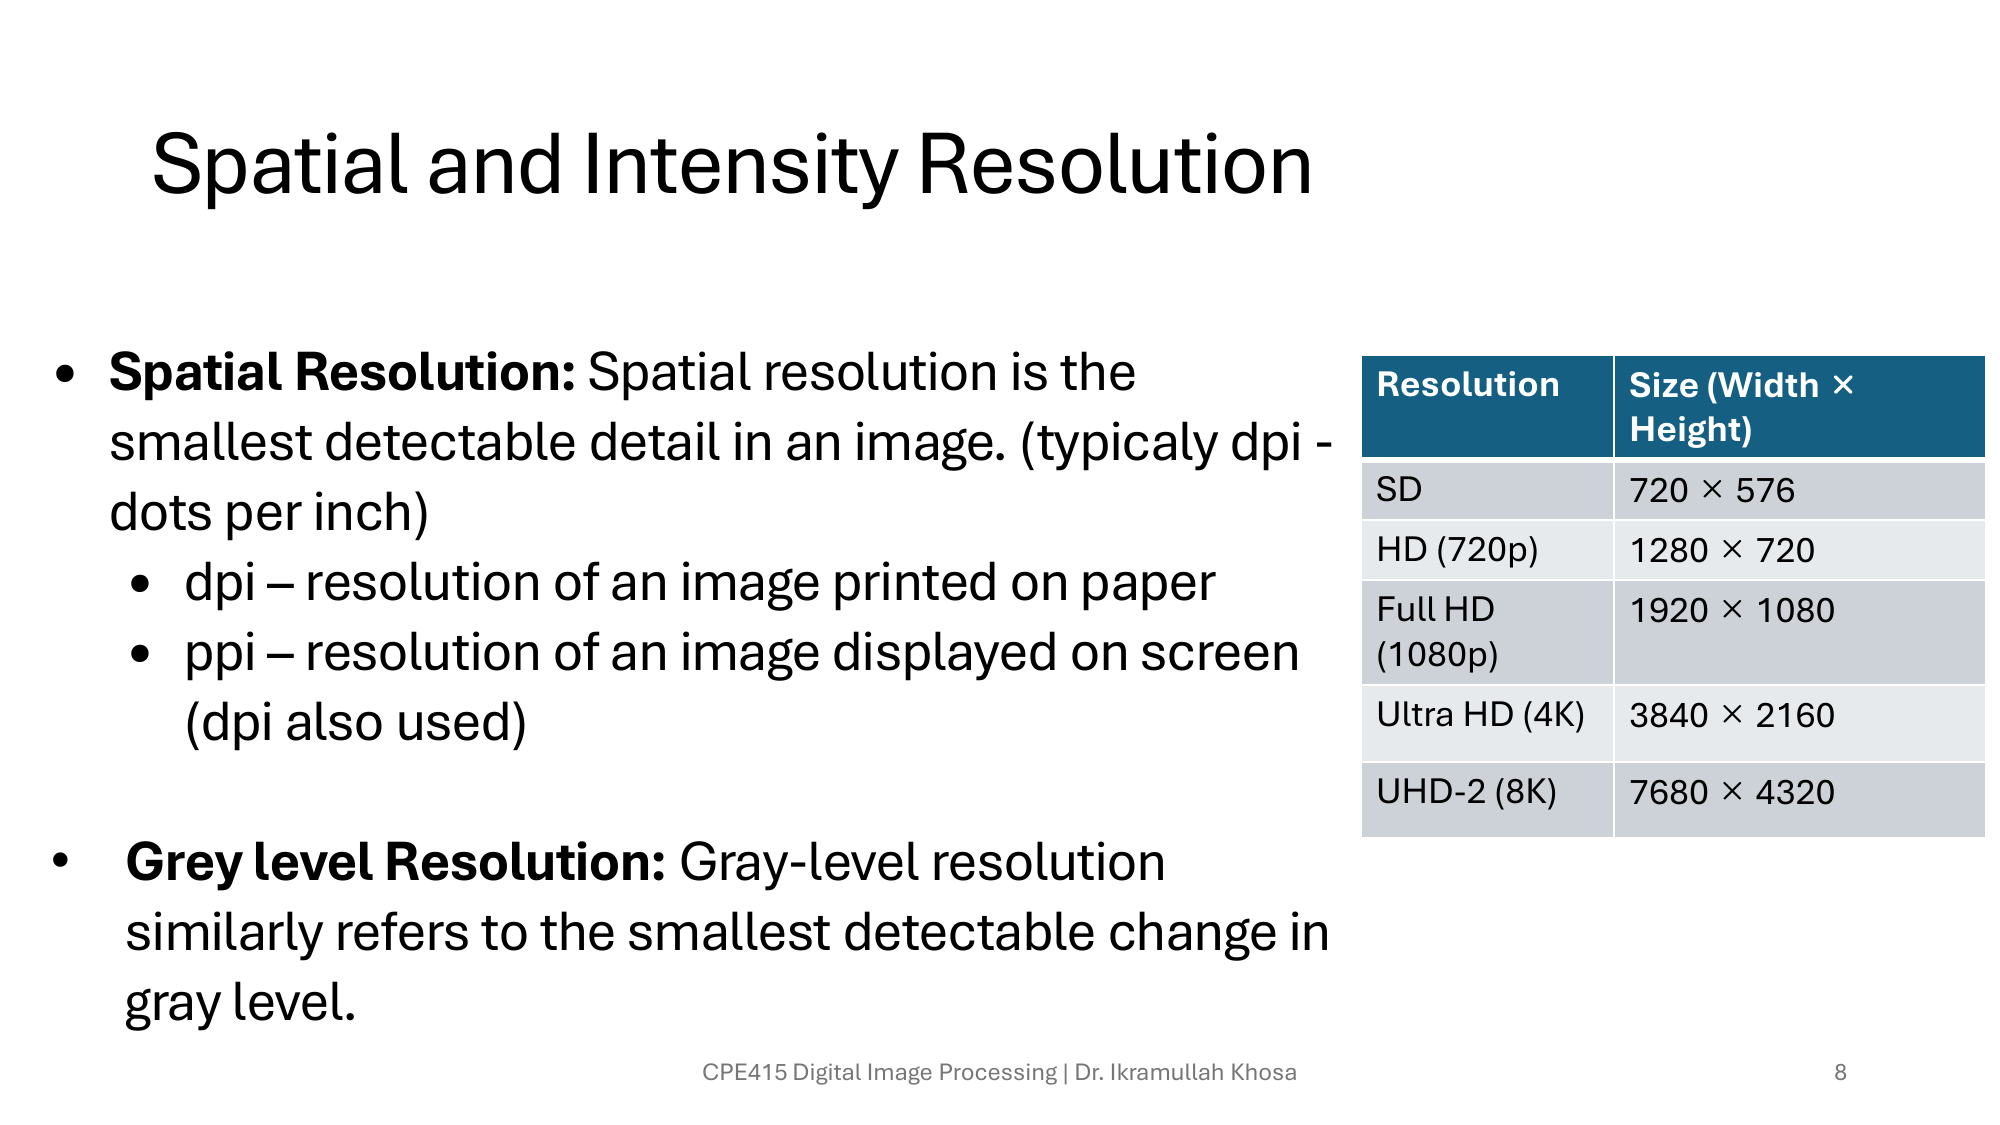
\includegraphics[width=0.85\textwidth]{images/slide3-08.png}
    \caption{Nearest neighbor interpolation}
    \label{fig:nn_interp}
\end{figure}

\begin{deepexplanation}
\textbf{DEEP ANALYSIS - Figure \ref{fig:nn_interp}: Nearest Neighbor Interpolation}

\textbf{The Algorithm:}
For a point at non-integer coordinates $(x, y)$:
\[
f(x, y) = f(\text{round}(x), \text{round}(y))
\]
Simply use the value of the \textbf{closest} pixel.

\textbf{Step-by-Step for Zooming by Factor $k$:}
\begin{enumerate}
    \item Create output image of size $kM \times kN$
    \item For each output pixel at $(i, j)$:
    \begin{itemize}
        \item Calculate corresponding input position: $(i/k, j/k)$
        \item Round to nearest integer: $(\text{round}(i/k), \text{round}(j/k))$
        \item Copy that input pixel to output
    \end{itemize}
\end{enumerate}

\textbf{Characteristics:}
\begin{center}
\begin{tabular}{|l|l|}
\hline
\textbf{Advantages} & \textbf{Disadvantages} \\
\hline
Fastest (simplest calculation) & Blocky appearance (``pixelation'') \\
Preserves original values & Jagged edges \\
No smoothing/blurring & Spatial aliasing artifacts \\
Sharp edges preserved & Poor for continuous-tone images \\
\hline
\end{tabular}
\end{center}

\textbf{When to Use:}
\begin{itemize}
    \item Zooming images for pixel-level inspection
    \item Binary or indexed-color images
    \item When speed is critical and quality is secondary
    \item When you want to see individual pixels clearly
\end{itemize}

\textbf{Mathematical Properties:}
\begin{itemize}
    \item Zero-order hold (piecewise constant)
    \item Frequency response: sinc function (poor anti-aliasing)
    \item Does not introduce new gray values
\end{itemize}
\end{deepexplanation}

\subsection{Bilinear Interpolation}

\begin{figure}[H]
    \centering
    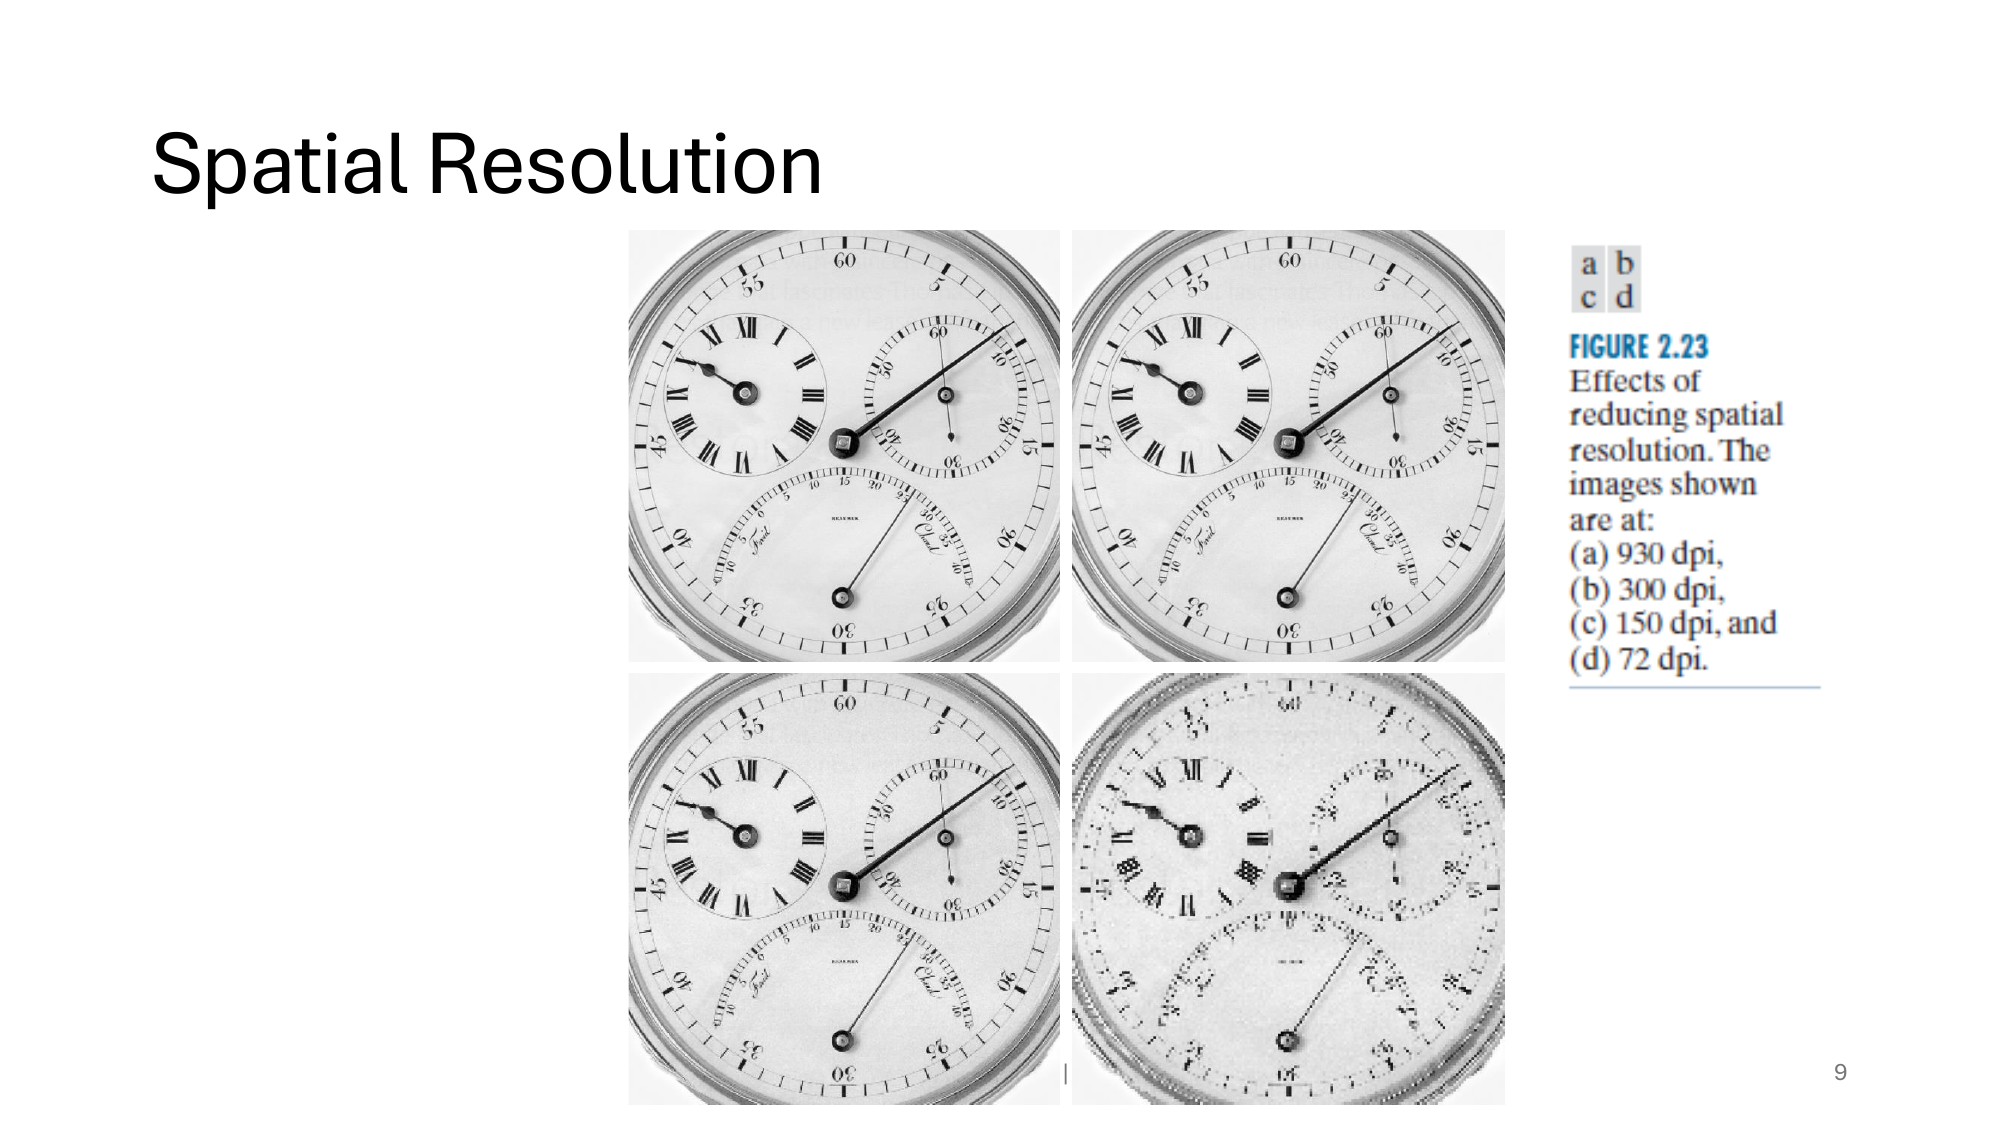
\includegraphics[width=0.85\textwidth]{images/slide3-09.png}
    \caption{Bilinear interpolation method}
    \label{fig:bilinear}
\end{figure}

\begin{deepexplanation}
\textbf{DEEP ANALYSIS - Figure \ref{fig:bilinear}: Bilinear Interpolation}

\textbf{The Concept:}
Use the \textbf{four nearest neighbors} and interpolate linearly in both $x$ and $y$ directions.

\textbf{The Formula:}
For point $(x, y)$ where $x = i + a$ and $y = j + b$ (with $0 \leq a, b < 1$):

Let the four neighbors be:
\begin{itemize}
    \item $f_{00} = f(i, j)$ --- top-left
    \item $f_{01} = f(i, j+1)$ --- top-right
    \item $f_{10} = f(i+1, j)$ --- bottom-left
    \item $f_{11} = f(i+1, j+1)$ --- bottom-right
\end{itemize}

Then:
\[
f(x, y) = (1-a)(1-b)f_{00} + (1-a)b \cdot f_{01} + a(1-b)f_{10} + ab \cdot f_{11}
\]

\textbf{Step-by-Step Process:}
\begin{enumerate}
    \item Interpolate in $x$ direction at top: $f_{top} = (1-b)f_{00} + b \cdot f_{01}$
    \item Interpolate in $x$ direction at bottom: $f_{bot} = (1-b)f_{10} + b \cdot f_{11}$
    \item Interpolate in $y$ direction: $f(x,y) = (1-a)f_{top} + a \cdot f_{bot}$
\end{enumerate}

\textbf{Characteristics:}
\begin{center}
\begin{tabular}{|l|l|}
\hline
\textbf{Advantages} & \textbf{Disadvantages} \\
\hline
Smooth results & Slight blurring \\
No blocky artifacts & Some loss of sharpness \\
Reasonably fast & Edges become slightly soft \\
Good quality/speed trade-off & Linear artifacts possible \\
\hline
\end{tabular}
\end{center}

\textbf{When to Use:}
\begin{itemize}
    \item General-purpose image resizing
    \item Real-time applications (video, games)
    \item When some blur is acceptable
    \item Good default choice for most applications
\end{itemize}
\end{deepexplanation}

\subsection{Bicubic Interpolation}

\begin{figure}[H]
    \centering
    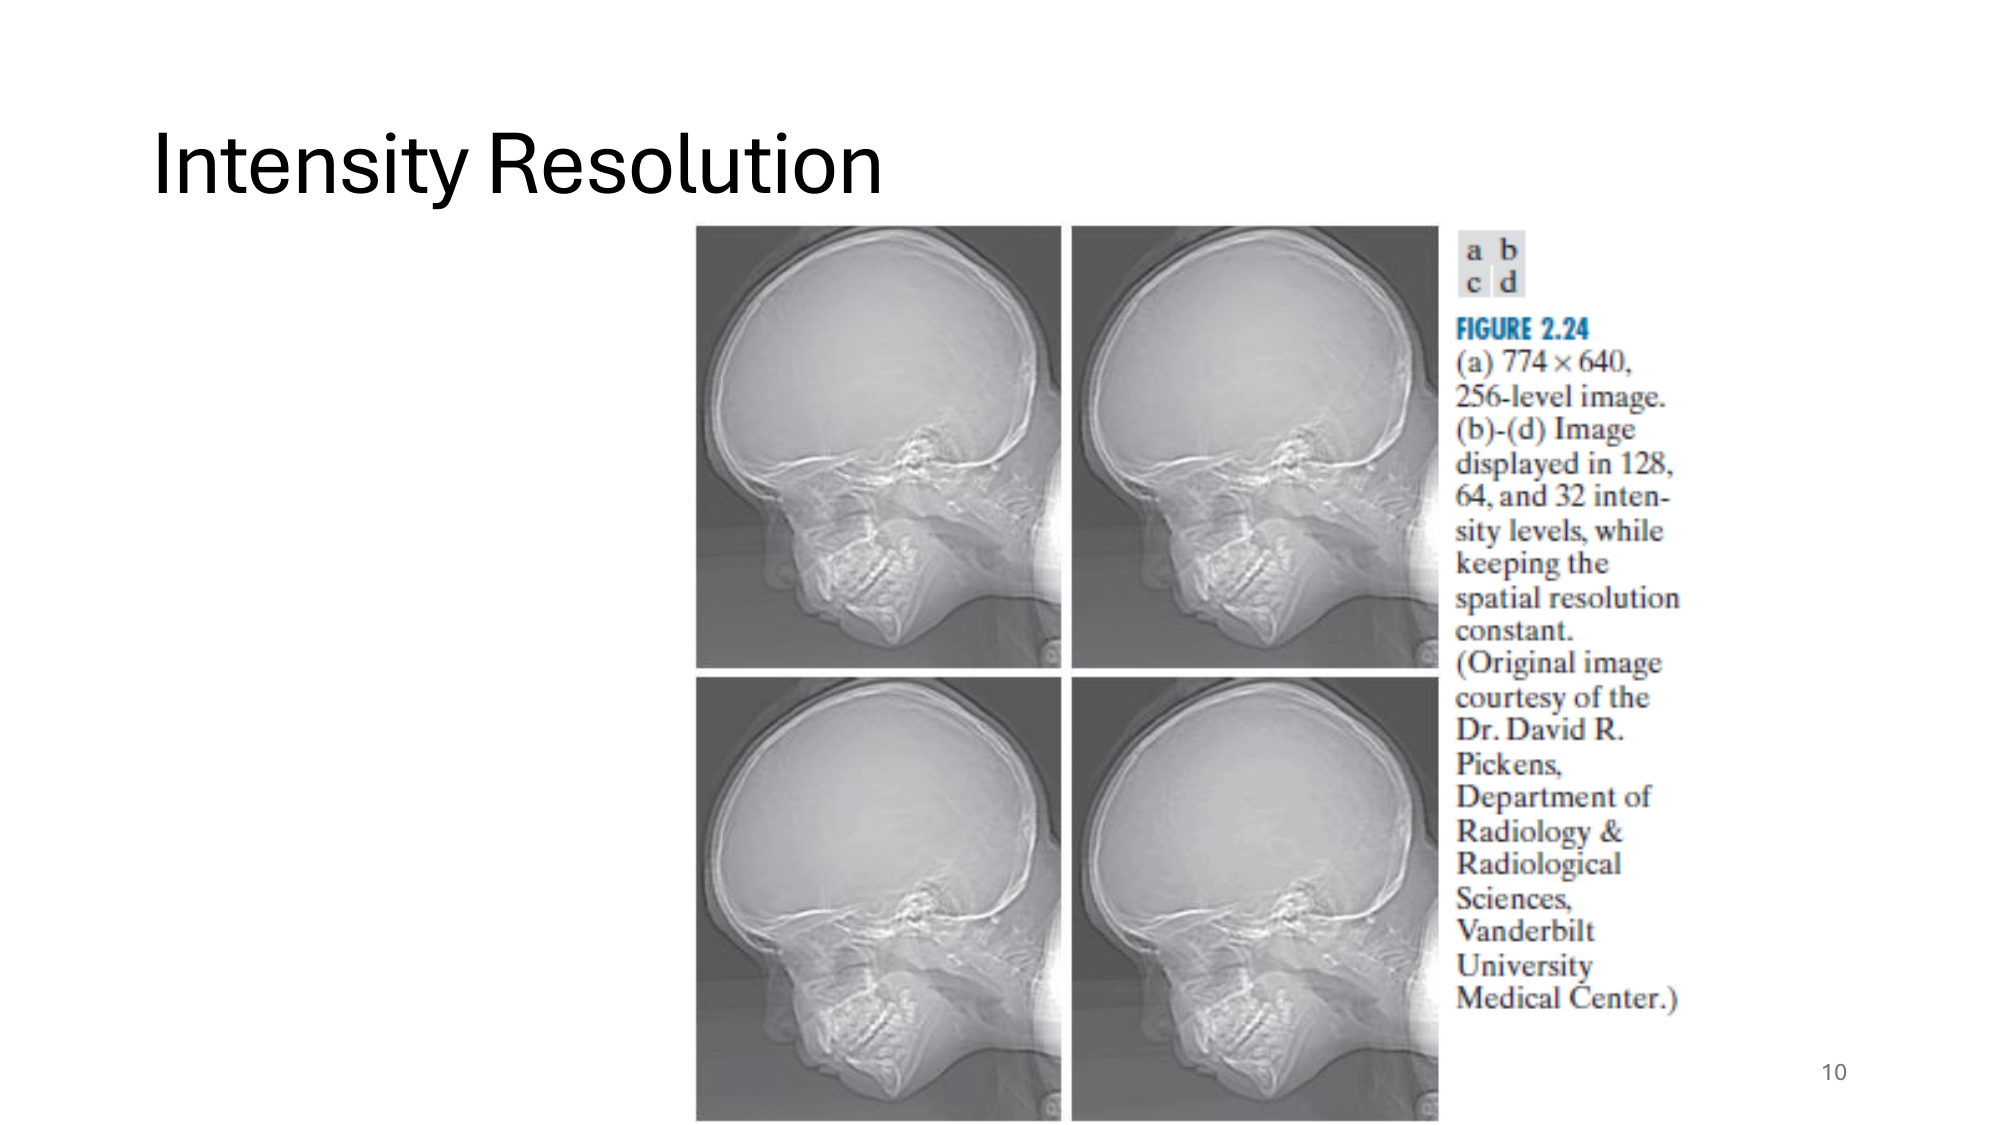
\includegraphics[width=0.85\textwidth]{images/slide3-10.png}
    \caption{Bicubic interpolation using 16 neighbors}
    \label{fig:bicubic}
\end{figure}

\begin{deepexplanation}
\textbf{DEEP ANALYSIS - Figure \ref{fig:bicubic}: Bicubic Interpolation}

\textbf{The Concept:}
Use \textbf{16 nearest neighbors} (4×4 grid) and fit a cubic polynomial surface.

\textbf{The Formula:}
\[
f(x, y) = \sum_{m=0}^{3} \sum_{n=0}^{3} a_{mn} x^m y^n
\]

Or using separable cubic convolution:
\[
f(x, y) = \sum_{i=-1}^{2} \sum_{j=-1}^{2} f(i, j) \cdot w(x-i) \cdot w(y-j)
\]

where $w(t)$ is the cubic weighting function:
\[
w(t) = \begin{cases}
(a+2)|t|^3 - (a+3)|t|^2 + 1 & \text{if } |t| \leq 1 \\
a|t|^3 - 5a|t|^2 + 8a|t| - 4a & \text{if } 1 < |t| < 2 \\
0 & \text{otherwise}
\end{cases}
\]
Typically $a = -0.5$ (Catmull-Rom) or $a = -1$ (cubic B-spline approximation).

\textbf{Characteristics:}
\begin{center}
\begin{tabular}{|l|l|}
\hline
\textbf{Advantages} & \textbf{Disadvantages} \\
\hline
Smoothest results & Slowest (16 samples) \\
Preserves edges better & Slight ringing at edges \\
Continuous first derivatives & More computation \\
Best quality for photos & Can create values outside input range \\
\hline
\end{tabular}
\end{center}

\textbf{Comparison Summary:}
\begin{center}
\begin{tabular}{|l|c|c|c|c|}
\hline
\textbf{Method} & \textbf{Neighbors} & \textbf{Speed} & \textbf{Quality} & \textbf{Blur} \\
\hline
Nearest & 1 & Fastest & Low & None \\
Bilinear & 4 & Fast & Medium & Some \\
Bicubic & 16 & Slow & High & Least \\
\hline
\end{tabular}
\end{center}

\textbf{When to Use:}
\begin{itemize}
    \item High-quality image enlargement
    \item Professional photo editing
    \item When computational cost is acceptable
    \item Printing/publication applications
\end{itemize}
\end{deepexplanation}

\begin{figure}[H]
    \centering
    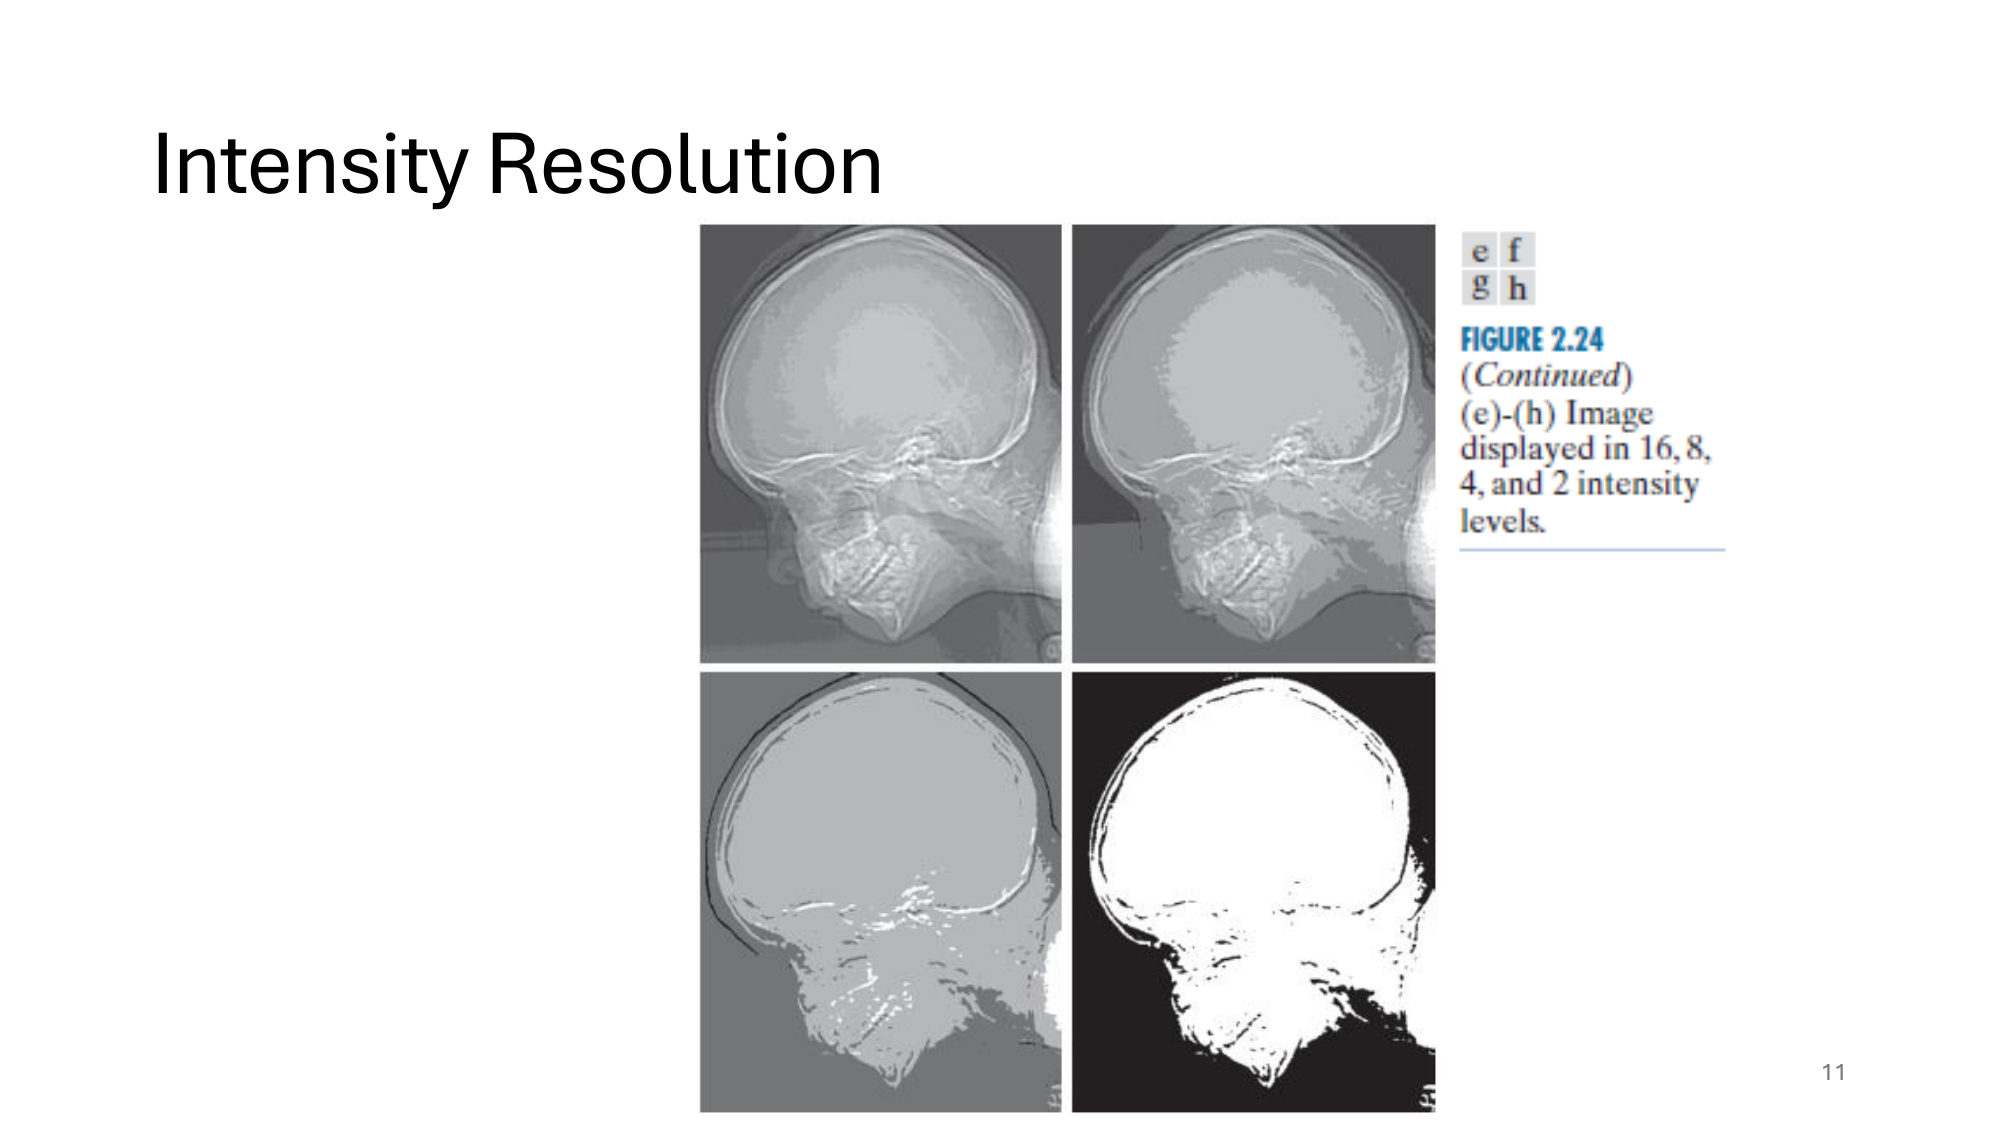
\includegraphics[width=0.9\textwidth]{images/slide3-11.png}
    \caption{Comparison of interpolation methods}
    \label{fig:interp_comparison}
\end{figure}

\begin{deepexplanation}
\textbf{DEEP ANALYSIS - Figure \ref{fig:interp_comparison}: Visual Comparison}

\textbf{What to Look For:}

\textbf{1. Nearest Neighbor:}
\begin{itemize}
    \item Blocky, stair-step appearance
    \item Original pixel boundaries clearly visible
    \item Diagonal lines show severe ``jaggies''
    \item Each enlarged ``pixel'' is a visible square
\end{itemize}

\textbf{2. Bilinear:}
\begin{itemize}
    \item Smoother than nearest neighbor
    \item Edges are slightly blurred
    \item No visible pixel blocks
    \item Good compromise appearance
\end{itemize}

\textbf{3. Bicubic:}
\begin{itemize}
    \item Smoothest overall appearance
    \item Edges remain relatively sharp
    \item May show slight ``ringing'' at high-contrast edges
    \item Most photorealistic result
\end{itemize}

\textbf{Why Bicubic Works Better:}
\begin{itemize}
    \item Uses more data points (16 vs. 4 vs. 1)
    \item Fits smoother function (cubic vs. linear vs. constant)
    \item Accounts for rate of change (derivative continuity)
\end{itemize}

\textbf{The Trade-off Triangle:}
\begin{itemize}
    \item Speed $\leftrightarrow$ Quality
    \item Sharpness $\leftrightarrow$ Smoothness
    \item Simplicity $\leftrightarrow$ Accuracy
\end{itemize}

No single method is best for all applications!
\end{deepexplanation}


%==============================================================================
\section{Relationships Between Pixels}
%==============================================================================

\subsection{Pixel Neighborhoods}

\begin{figure}[H]
    \centering
    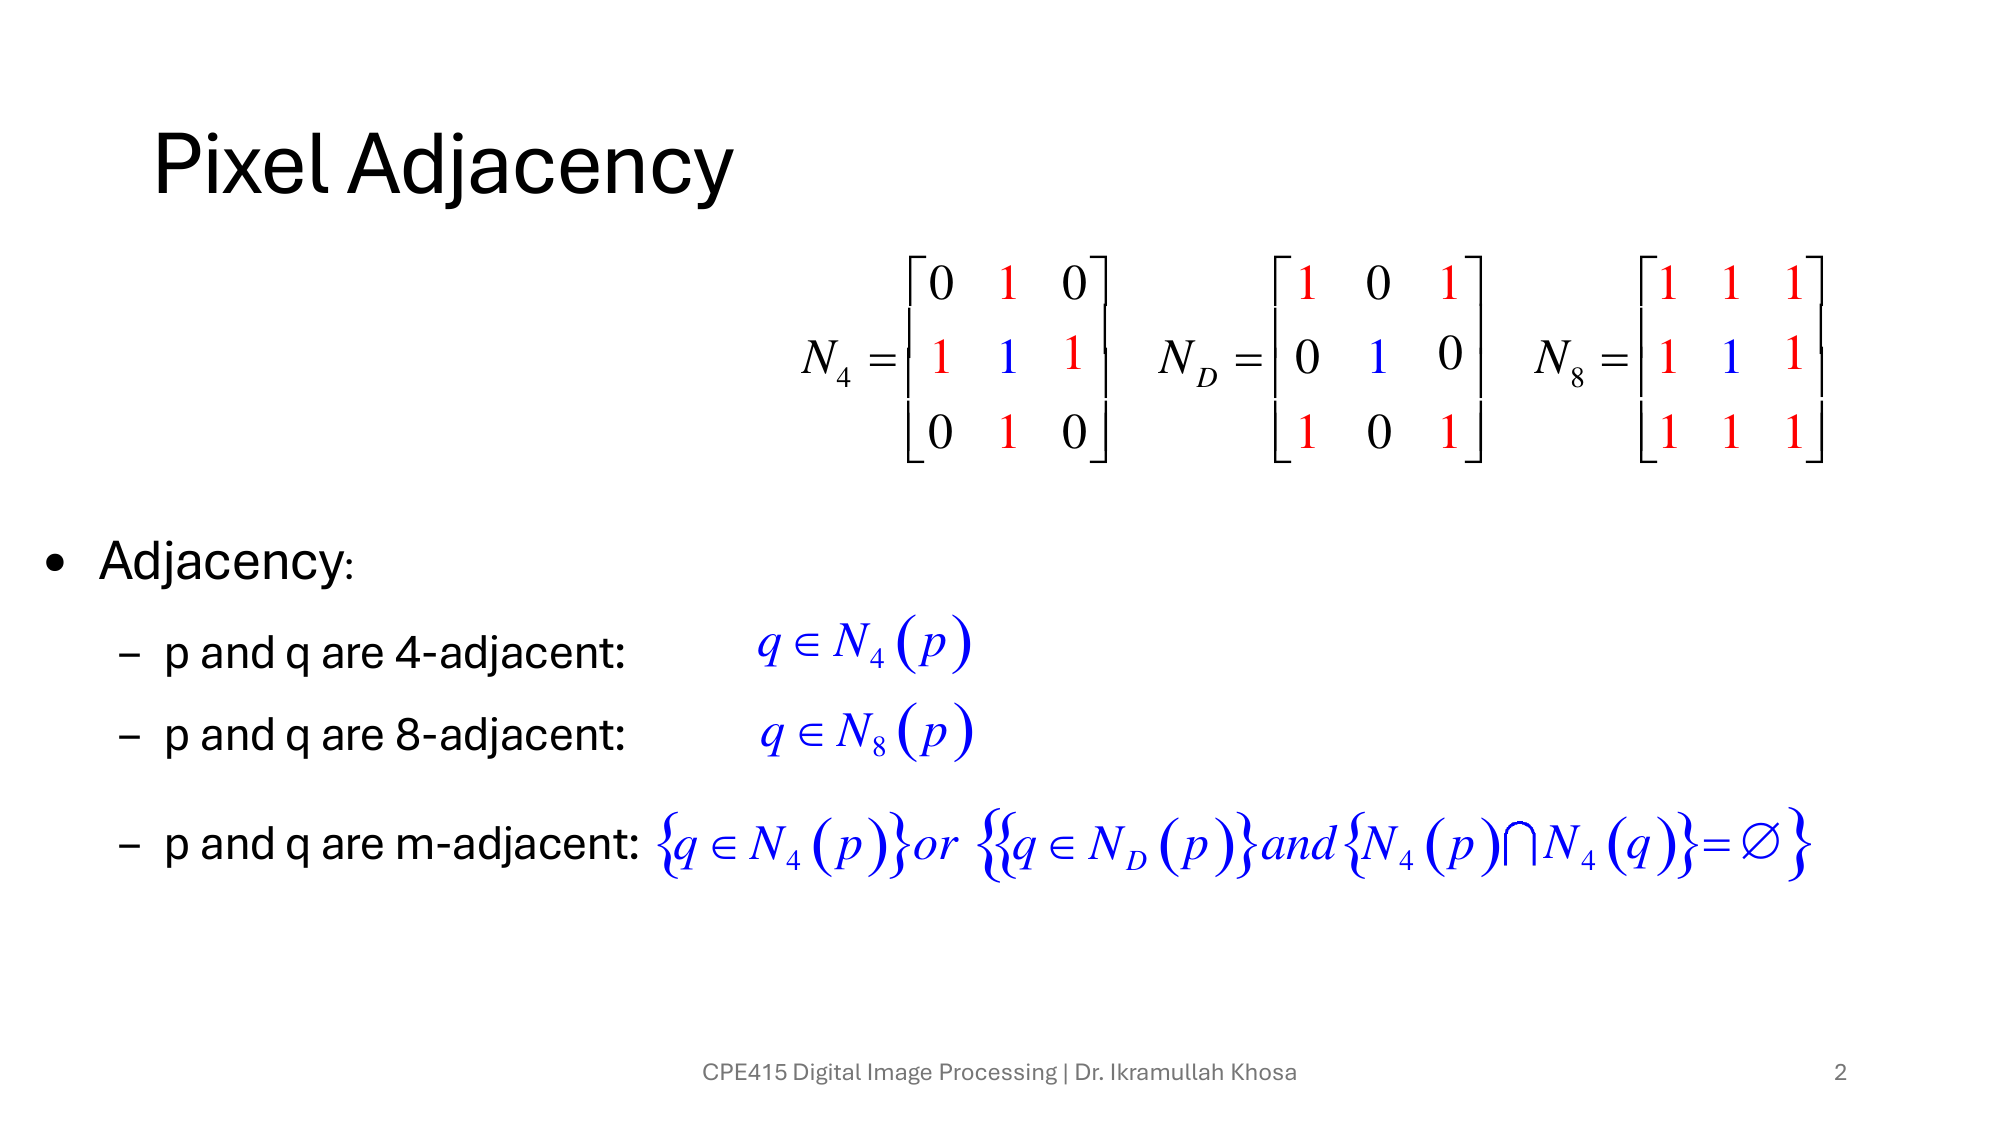
\includegraphics[width=0.85\textwidth]{images/slide4-02.png}
    \caption{4-neighborhood and 8-neighborhood of a pixel}
    \label{fig:neighborhoods}
\end{figure}

\begin{deepexplanation}
\textbf{DEEP ANALYSIS - Figure \ref{fig:neighborhoods}: Defining Pixel Neighbors}

\textbf{The Three Neighborhood Types:}

\textbf{1. 4-Neighborhood $N_4(p)$:}
For pixel $p$ at $(x, y)$, the 4-neighbors are:
\[
N_4(p) = \{(x-1, y), (x+1, y), (x, y-1), (x, y+1)\}
\]
\begin{itemize}
    \item Horizontally and vertically adjacent pixels
    \item Also called ``direct neighbors'' or ``von Neumann neighborhood''
    \item Distance from $p$: exactly 1 pixel
\end{itemize}

\textbf{2. Diagonal Neighbors $N_D(p)$:}
\[
N_D(p) = \{(x-1, y-1), (x-1, y+1), (x+1, y-1), (x+1, y+1)\}
\]
\begin{itemize}
    \item The four diagonal neighbors
    \item Distance from $p$: $\sqrt{2} \approx 1.414$ pixels
\end{itemize}

\textbf{3. 8-Neighborhood $N_8(p)$:}
\[
N_8(p) = N_4(p) \cup N_D(p)
\]
\begin{itemize}
    \item All surrounding pixels (both direct and diagonal)
    \item Also called ``Moore neighborhood''
    \item 8 pixels total (or fewer at image boundaries)
\end{itemize}

\textbf{Visual Representation:}
\begin{center}
\begin{tabular}{|c|c|c|}
\hline
$N_D$ & $N_4$ & $N_D$ \\
\hline
$N_4$ & $p$ & $N_4$ \\
\hline
$N_D$ & $N_4$ & $N_D$ \\
\hline
\end{tabular}
\end{center}

\textbf{Why These Definitions Matter:}
\begin{itemize}
    \item Connectivity (what counts as ``connected'')
    \item Edge detection and contour following
    \item Region growing and segmentation
    \item Morphological operations
\end{itemize}
\end{deepexplanation}

\subsection{Pixel Adjacency and Connectivity}

\begin{figure}[H]
    \centering
    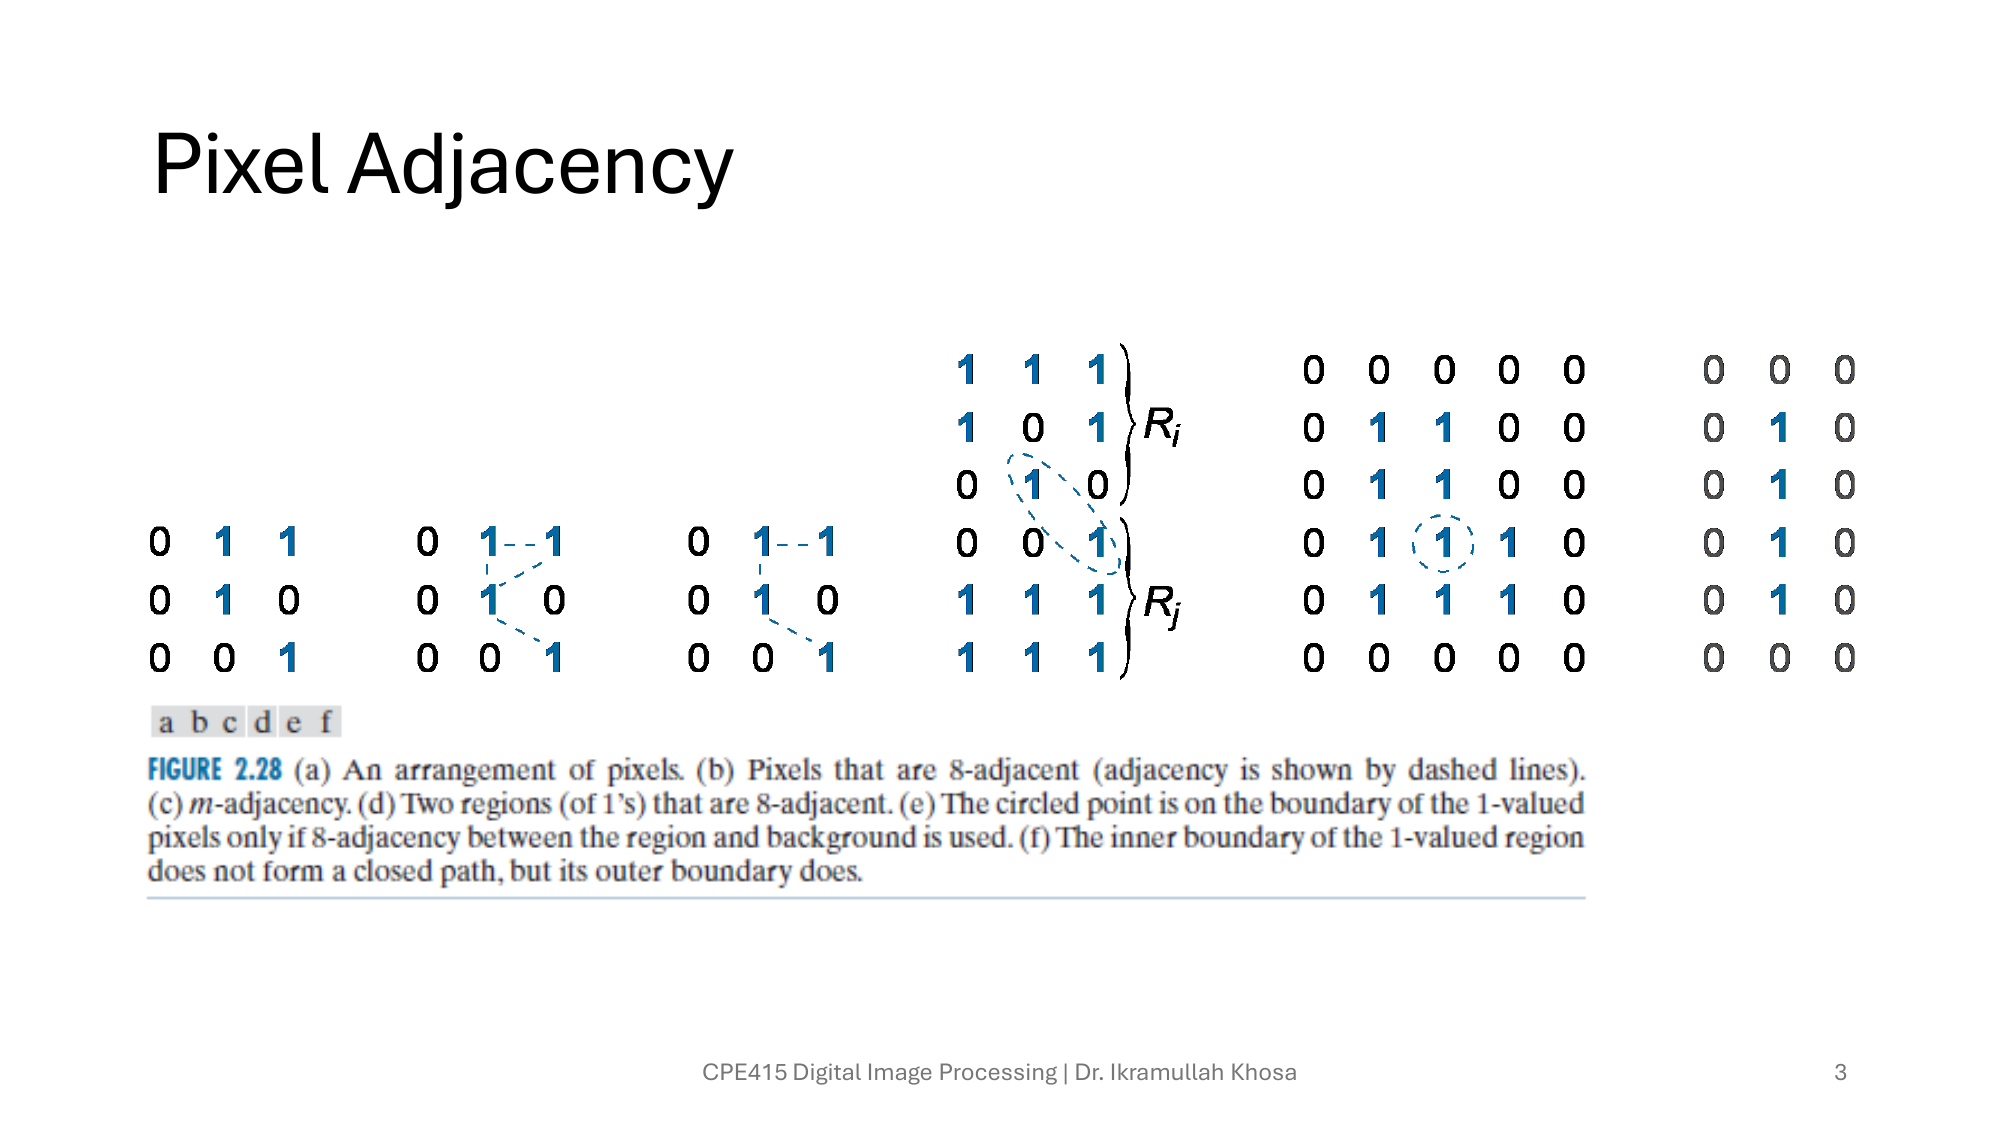
\includegraphics[width=0.85\textwidth]{images/slide4-03.png}
    \caption{Different types of adjacency}
    \label{fig:adjacency}
\end{figure}

\begin{deepexplanation}
\textbf{DEEP ANALYSIS - Figure \ref{fig:adjacency}: Adjacency Types}

\textbf{The Definition of Adjacency:}
Two pixels $p$ and $q$ are \textbf{adjacent} if:
\begin{enumerate}
    \item They are neighbors (in some neighborhood sense)
    \item Their values satisfy a similarity criterion $V$
\end{enumerate}

\textbf{The Similarity Set $V$:}
\begin{itemize}
    \item $V$ = set of intensity values that define ``similar''
    \item Example: $V = \{1\}$ (both pixels must have value 1)
    \item Example: $V = \{100, 101, 102\}$ (values within 2 of each other)
    \item For binary images: $V = \{1\}$ (the foreground value)
\end{itemize}

\textbf{Three Types of Adjacency:}

\textbf{1. 4-Adjacency:}
\begin{itemize}
    \item $p$ and $q$ are 4-adjacent if $q \in N_4(p)$ and their values are in $V$
\end{itemize}

\textbf{2. 8-Adjacency:}
\begin{itemize}
    \item $p$ and $q$ are 8-adjacent if $q \in N_8(p)$ and their values are in $V$
\end{itemize}

\textbf{3. m-Adjacency (Mixed):}
\begin{itemize}
    \item $p$ and $q$ are m-adjacent if:
    \begin{enumerate}
        \item $q \in N_4(p)$ and values in $V$, OR
        \item $q \in N_D(p)$ and values in $V$, AND $N_4(p) \cap N_4(q) \cap V = \emptyset$
    \end{enumerate}
\end{itemize}

\textbf{Why m-Adjacency?}
Eliminates \textbf{ambiguous connectivity} that can occur with 8-adjacency.
\end{deepexplanation}

\begin{figure}[H]
    \centering
    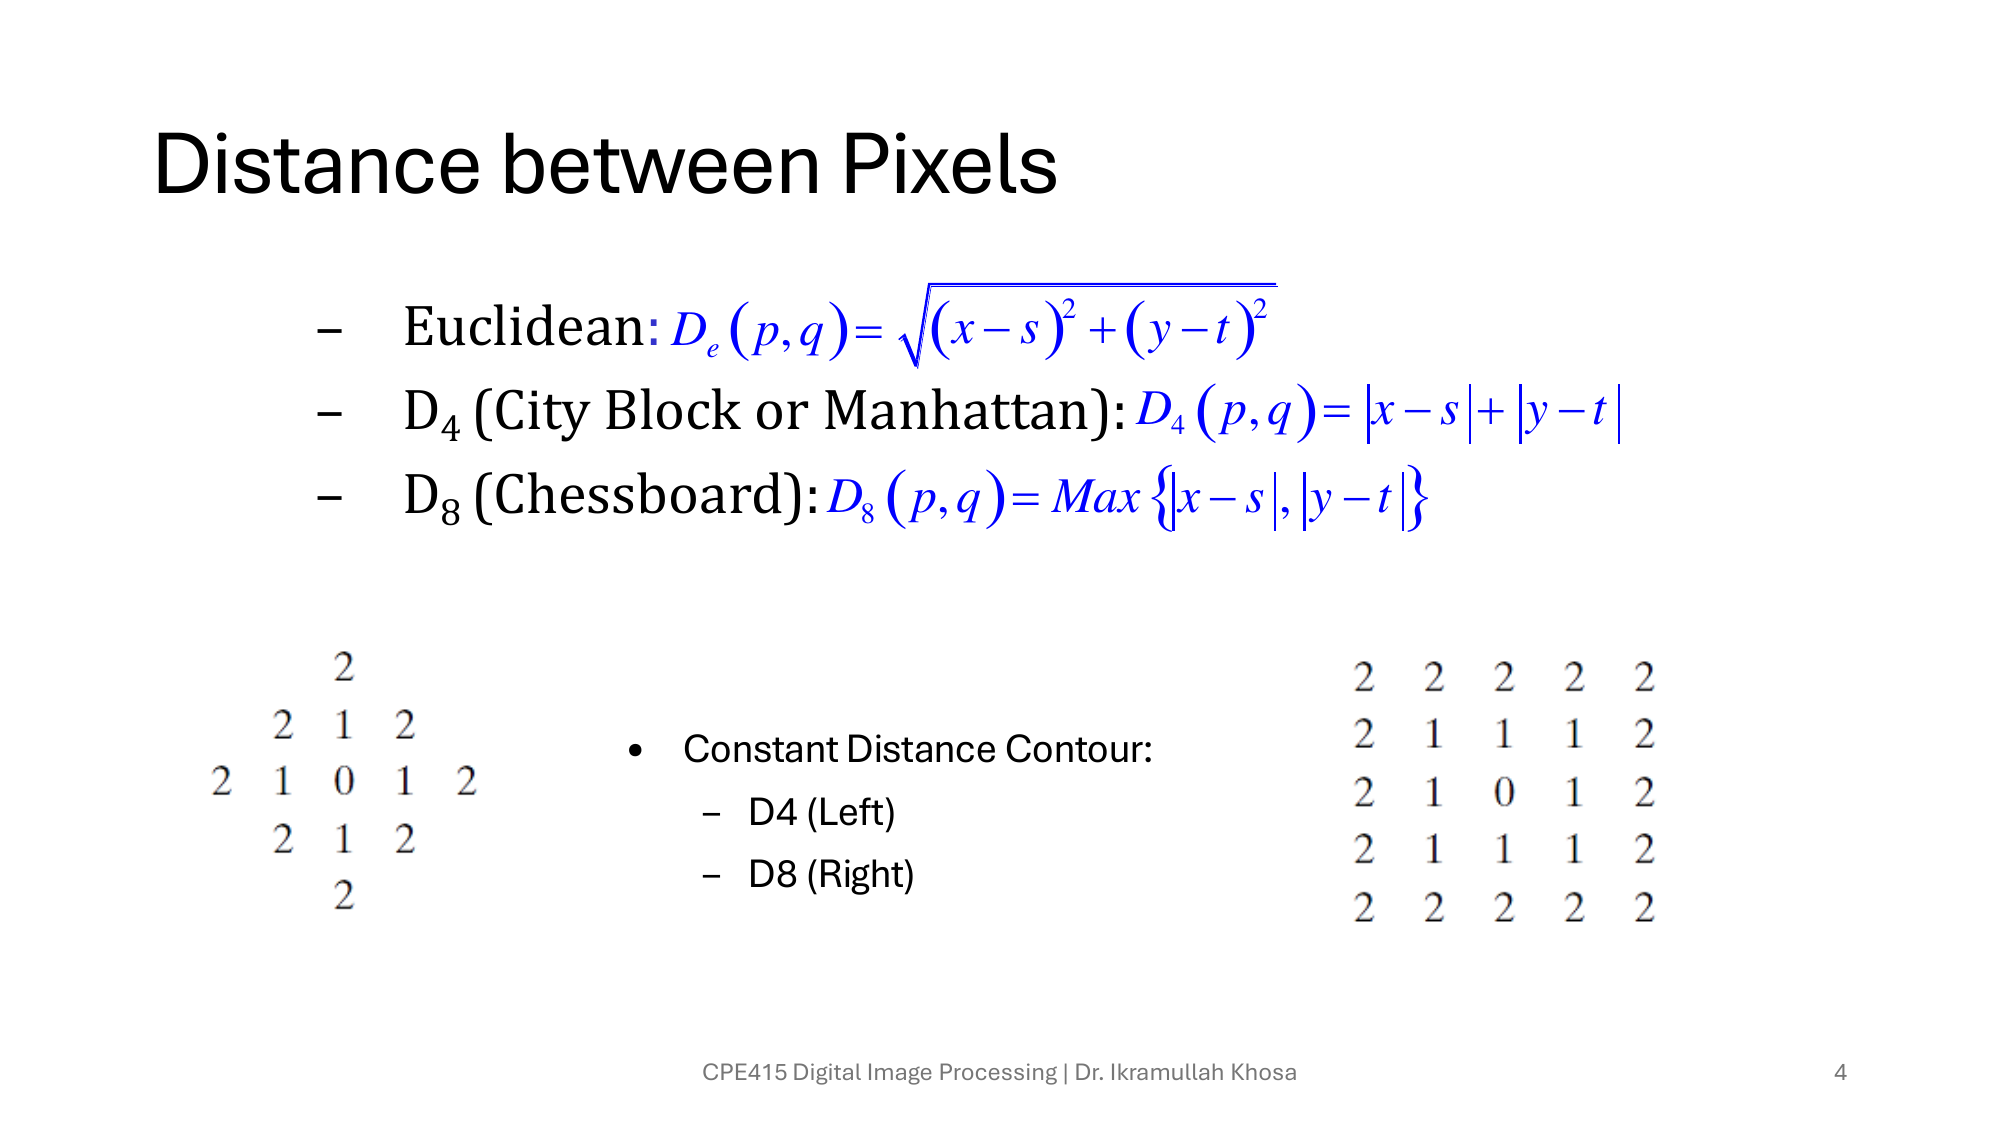
\includegraphics[width=0.85\textwidth]{images/slide4-04.png}
    \caption{m-adjacency explained}
    \label{fig:m_adjacency}
\end{figure}

\begin{deepexplanation}
\textbf{DEEP ANALYSIS - Figure \ref{fig:m_adjacency}: The m-Adjacency Problem and Solution}

\textbf{The Problem with 8-Adjacency:}
Consider four pixels in a 2×2 square, all with value in $V$:
\begin{center}
\begin{tabular}{|c|c|}
\hline
1 & 1 \\
\hline
1 & 1 \\
\hline
\end{tabular}
\end{center}

With 8-adjacency, there are \textbf{multiple paths} between corners:
\begin{itemize}
    \item Top-left to bottom-right: Direct diagonal, OR via top-right, OR via bottom-left
    \item This creates \textbf{ambiguous connectivity}
\end{itemize}

\textbf{The m-Adjacency Solution:}
\begin{itemize}
    \item Only allow diagonal connection when NO 4-connected path exists
    \item In the 2×2 example: Top-left and bottom-right are NOT m-adjacent
    \item Why? They share 4-neighbors (top-right and bottom-left) that are also in $V$
\end{itemize}

\textbf{m-Adjacency Rule:}
``Use diagonal connections only when necessary --- prefer 4-connectivity when possible.''

\textbf{Formal Definition:}
$p$ and $q$ are m-adjacent if both values are in $V$ AND either:
\begin{enumerate}
    \item $q \in N_4(p)$ (they're 4-neighbors), OR
    \item $q \in N_D(p)$ AND they have no common 4-neighbor with value in $V$
\end{enumerate}

\textbf{Benefit:}
\begin{itemize}
    \item Unique path between any two connected points
    \item No ambiguity in connectivity
    \item Better for algorithms that trace boundaries or count objects
\end{itemize}
\end{deepexplanation}

\subsection{Connectivity and Paths}

\begin{figure}[H]
    \centering
    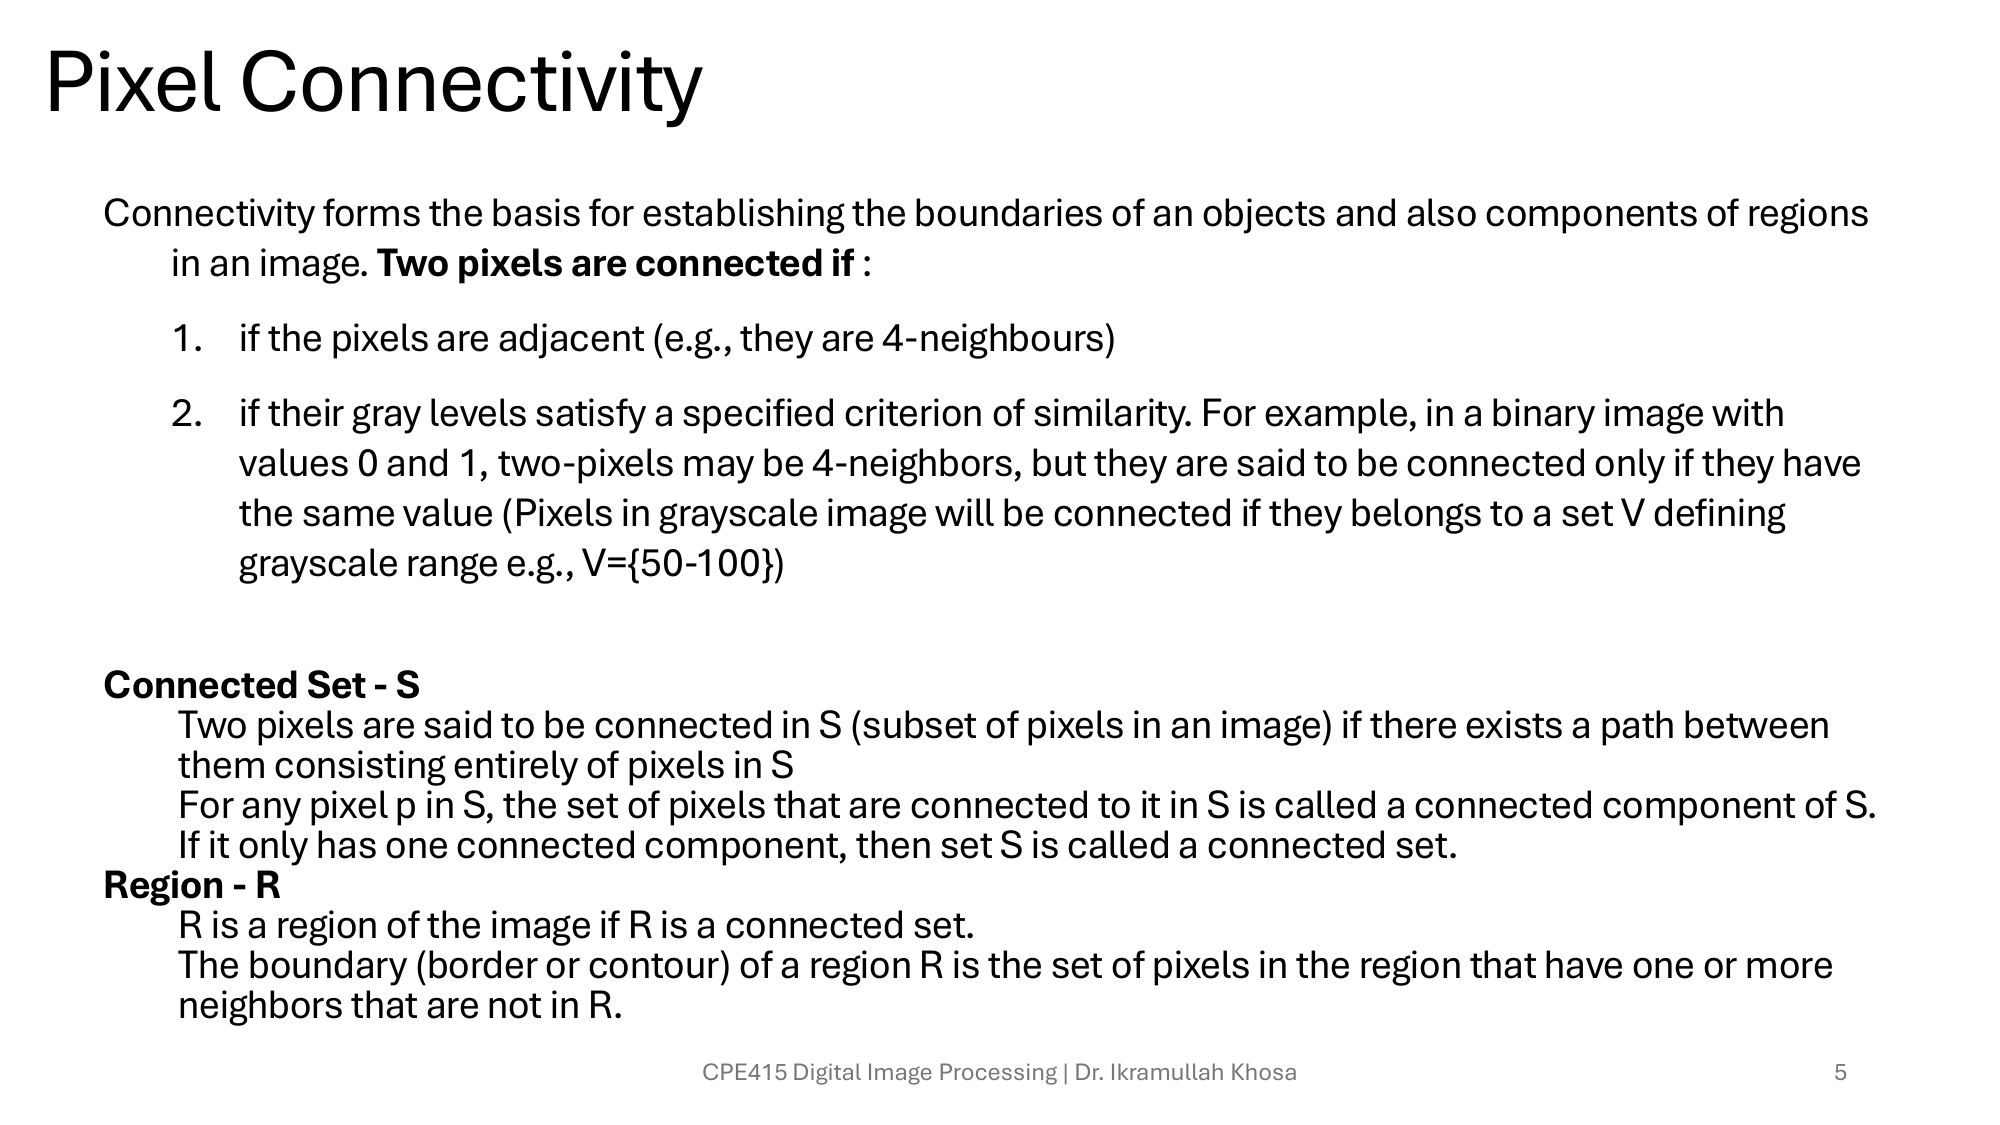
\includegraphics[width=0.85\textwidth]{images/slide4-05.png}
    \caption{Paths and connectivity in images}
    \label{fig:paths}
\end{figure}

\begin{deepexplanation}
\textbf{DEEP ANALYSIS - Figure \ref{fig:paths}: Paths Through Pixels}

\textbf{Definition of a Path:}
A \textbf{path} from pixel $p = (x_0, y_0)$ to pixel $q = (x_n, y_n)$ is a sequence of pixels:
\[
(x_0, y_0), (x_1, y_1), \ldots, (x_n, y_n)
\]
where $(x_i, y_i)$ and $(x_{i+1}, y_{i+1})$ are adjacent for all $i$.

\textbf{Types of Paths (Based on Adjacency):}
\begin{itemize}
    \item \textbf{4-path}: Uses only 4-adjacency (horizontal/vertical moves)
    \item \textbf{8-path}: Uses 8-adjacency (can move diagonally)
    \item \textbf{m-path}: Uses m-adjacency
\end{itemize}

\textbf{Path Length:}
\begin{itemize}
    \item The number of pixels in the path (including endpoints)
    \item Or: The number of steps (path length minus 1)
\end{itemize}

\textbf{Closed Path:}
A path where $(x_0, y_0) = (x_n, y_n)$ --- forms a loop.

\textbf{Connectivity (The Key Concept):}
Two pixels $p$ and $q$ are \textbf{connected} if there exists a path between them (with all pixels in $V$).

\textbf{Connected Component:}
\begin{itemize}
    \item A maximal set of mutually connected pixels
    \item Every pixel in the set is connected to every other
    \item No pixel outside the set is connected to pixels inside
\end{itemize}

\textbf{Application Examples:}
\begin{itemize}
    \item Object counting: Each connected component = one object
    \item Region labeling: Assign unique ID to each component
    \item Hole detection: Background components inside objects
\end{itemize}
\end{deepexplanation}

\subsection{Distance Measures}

\begin{figure}[H]
    \centering
    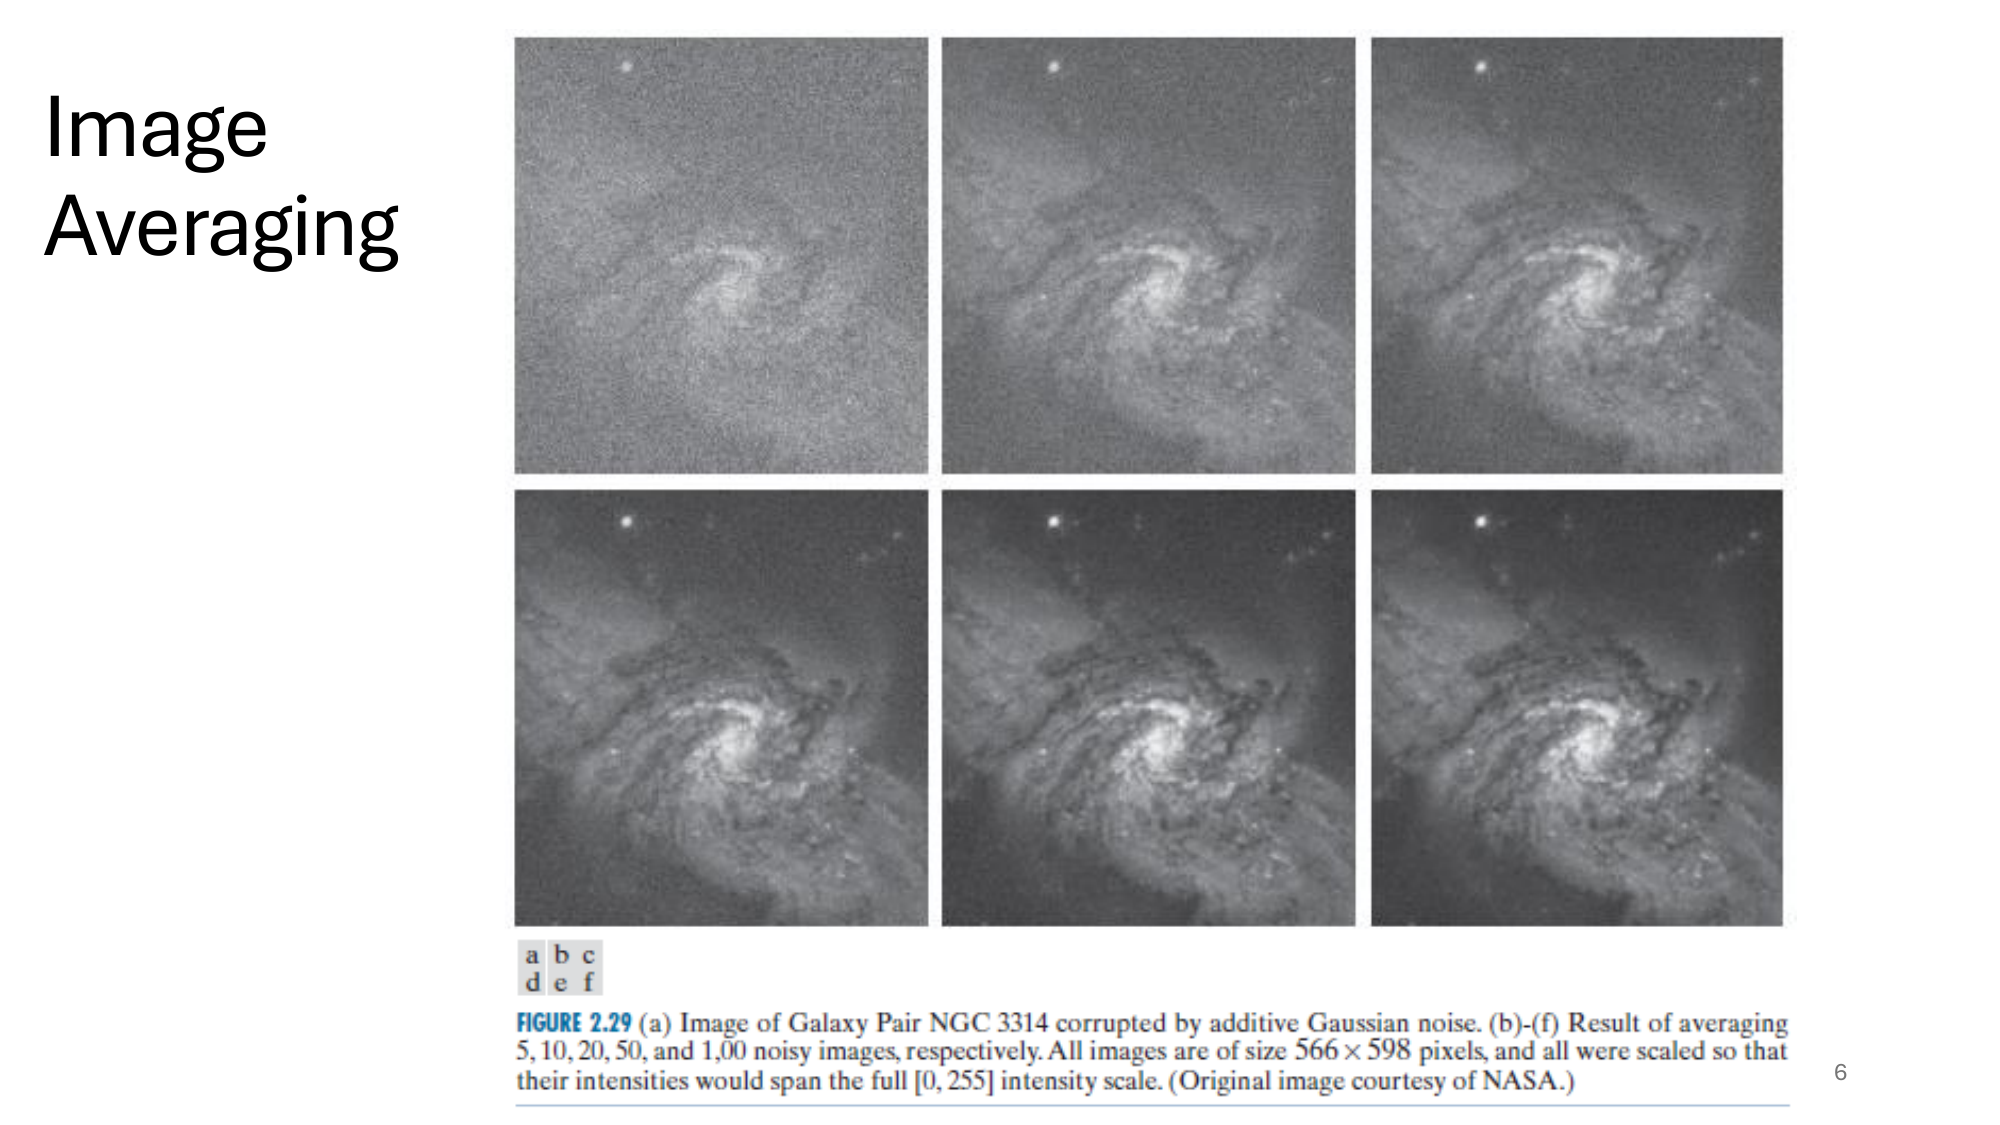
\includegraphics[width=0.85\textwidth]{images/slide4-06.png}
    \caption{Different distance metrics}
    \label{fig:distances}
\end{figure}

\begin{deepexplanation}
\textbf{DEEP ANALYSIS - Figure \ref{fig:distances}: Measuring Distance Between Pixels}

\textbf{Three Common Distance Metrics:}

For pixels $p = (x_1, y_1)$ and $q = (x_2, y_2)$:

\textbf{1. Euclidean Distance $D_E$:}
\[
D_E(p, q) = \sqrt{(x_1 - x_2)^2 + (y_1 - y_2)^2}
\]
\begin{itemize}
    \item The ``ordinary'' straight-line distance
    \item Can be any non-negative real number
    \item Computationally expensive (square root)
\end{itemize}

\textbf{2. City-Block Distance $D_4$ (Manhattan Distance):}
\[
D_4(p, q) = |x_1 - x_2| + |y_1 - y_2|
\]
\begin{itemize}
    \item Distance traveling only horizontally/vertically
    \item Like walking on a city grid
    \item Always an integer for integer coordinates
    \item Pixels with $D_4 = 1$ are the 4-neighbors
\end{itemize}

\textbf{3. Chessboard Distance $D_8$ (Chebyshev Distance):}
\[
D_8(p, q) = \max(|x_1 - x_2|, |y_1 - y_2|)
\]
\begin{itemize}
    \item Minimum moves for a chess king
    \item Can move diagonally (counts as 1 step)
    \item Pixels with $D_8 = 1$ are the 8-neighbors
\end{itemize}

\textbf{Comparison for Point $(3, 0)$ from Origin:}
\begin{center}
\begin{tabular}{|l|c|}
\hline
\textbf{Metric} & \textbf{Distance} \\
\hline
$D_E$ & $\sqrt{9} = 3.0$ \\
$D_4$ & $3 + 0 = 3$ \\
$D_8$ & $\max(3, 0) = 3$ \\
\hline
\end{tabular}
\end{center}

\textbf{For Point $(3, 3)$ from Origin:}
\begin{center}
\begin{tabular}{|l|c|}
\hline
$D_E$ & $\sqrt{18} \approx 4.24$ \\
$D_4$ & $3 + 3 = 6$ \\
$D_8$ & $\max(3, 3) = 3$ \\
\hline
\end{tabular}
\end{center}

\textbf{Relationship:}
\[
D_8(p, q) \leq D_E(p, q) \leq D_4(p, q)
\]
(Chessboard is always smallest, city-block always largest or equal)
\end{deepexplanation}

\begin{figure}[H]
    \centering
    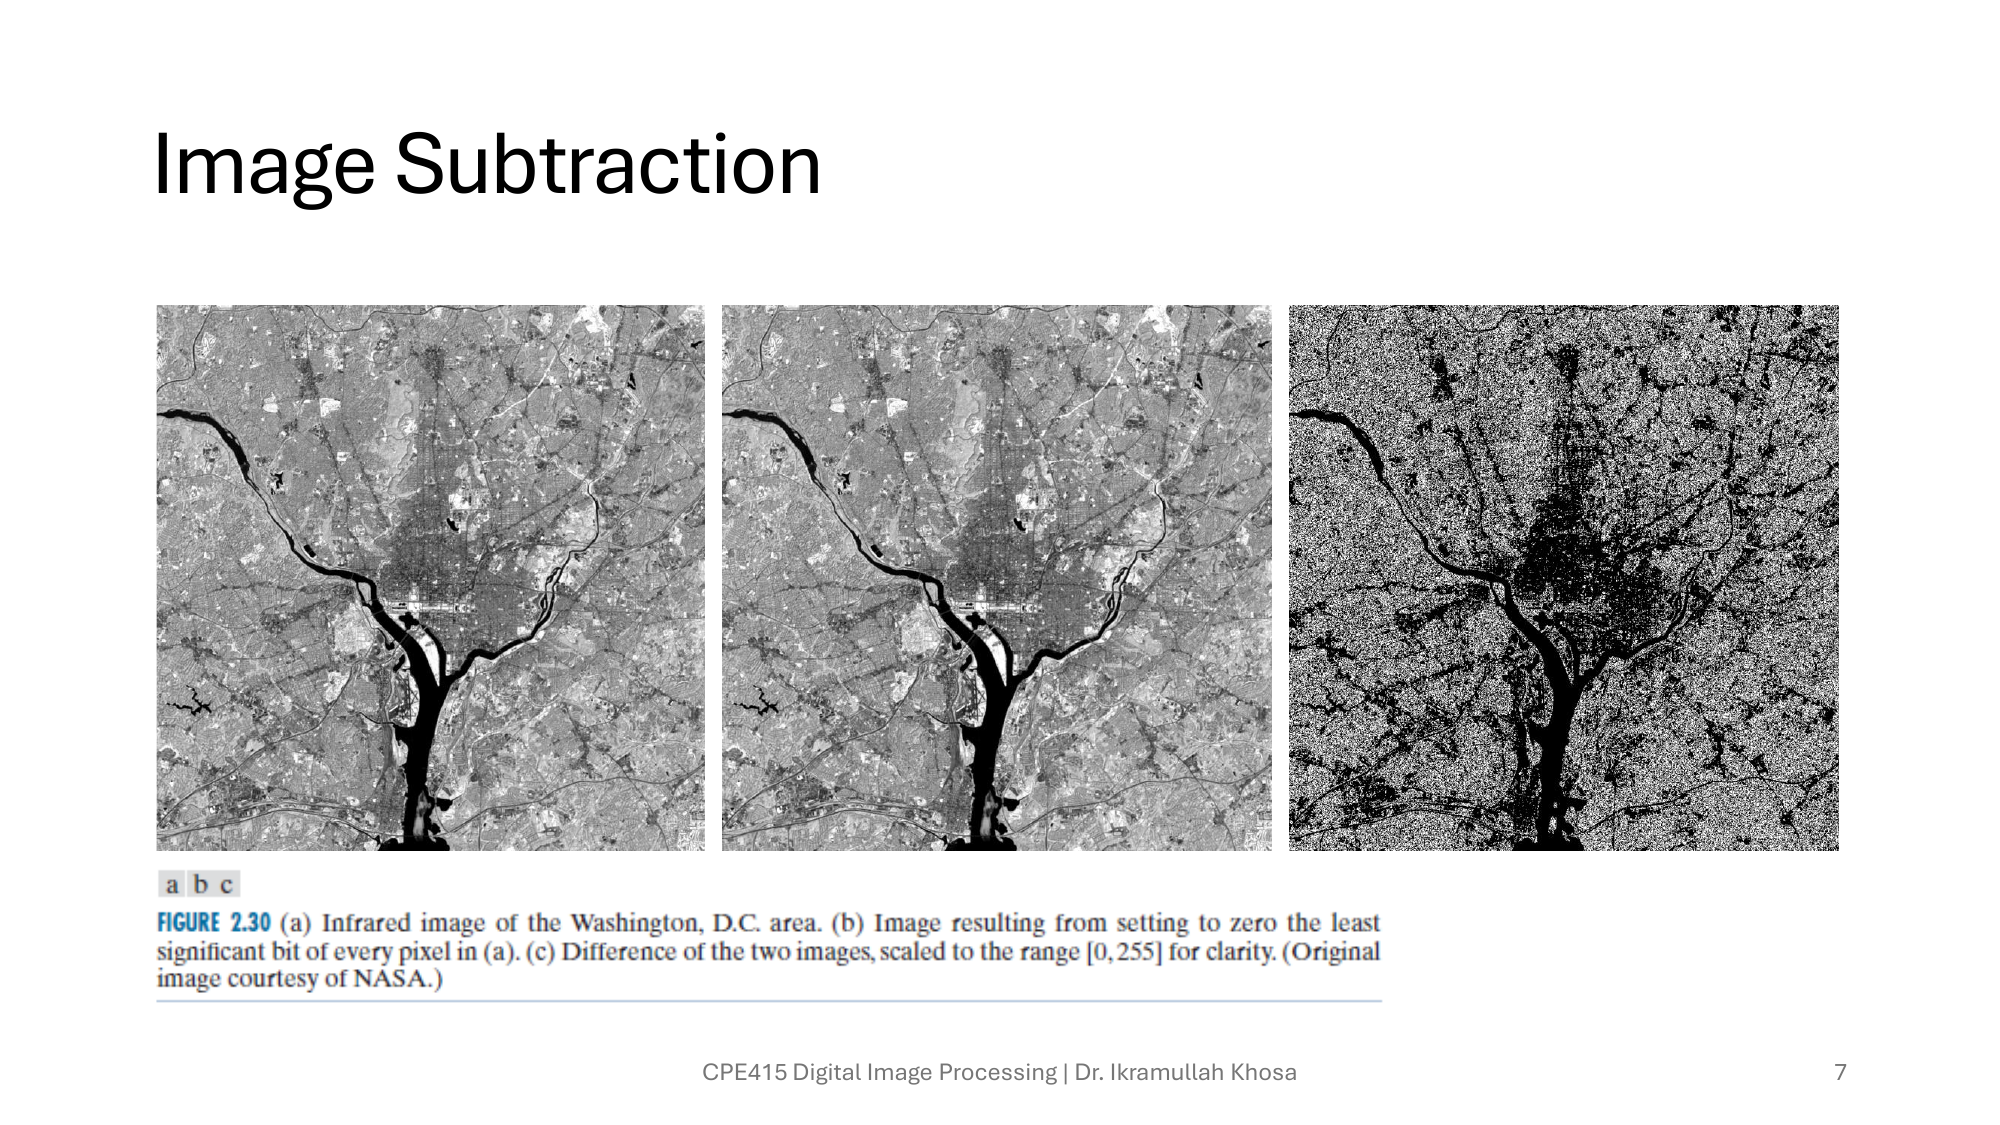
\includegraphics[width=0.85\textwidth]{images/slide4-07.png}
    \caption{Distance ``circles'' for different metrics}
    \label{fig:distance_circles}
\end{figure}

\begin{deepexplanation}
\textbf{DEEP ANALYSIS - Figure \ref{fig:distance_circles}: Shape of Distance Balls}

\textbf{What the Figure Shows:}
All pixels at distance $\leq r$ from a center point (``distance ball'' or ``disk'').

\textbf{Euclidean Distance ($D_E$):}
\begin{itemize}
    \item Produces a true \textbf{circle}
    \item Rotationally symmetric
    \item Most intuitive geometrically
\end{itemize}

\textbf{City-Block Distance ($D_4$):}
\begin{itemize}
    \item Produces a \textbf{diamond} (rotated square)
    \item Axes aligned with coordinate axes
    \item Points on boundary: $|x| + |y| = r$
\end{itemize}

\textbf{Chessboard Distance ($D_8$):}
\begin{itemize}
    \item Produces a \textbf{square}
    \item Axes aligned with coordinate axes
    \item Points on boundary: $\max(|x|, |y|) = r$
\end{itemize}

\textbf{Practical Implications:}
\begin{itemize}
    \item $D_E$: Use for accurate geometric measurements
    \item $D_4$: Fast computation, used in distance transforms
    \item $D_8$: Good for morphological operations, region growing
\end{itemize}

\textbf{The Distance Transform:}
Replace each pixel with its distance to the nearest boundary:
\begin{itemize}
    \item Useful for skeletonization
    \item Finding medial axis
    \item Object separation
\end{itemize}
\end{deepexplanation}

%==============================================================================
\section{Basic Image Operations}
%==============================================================================

\subsection{Arithmetic Operations}

\begin{figure}[H]
    \centering
    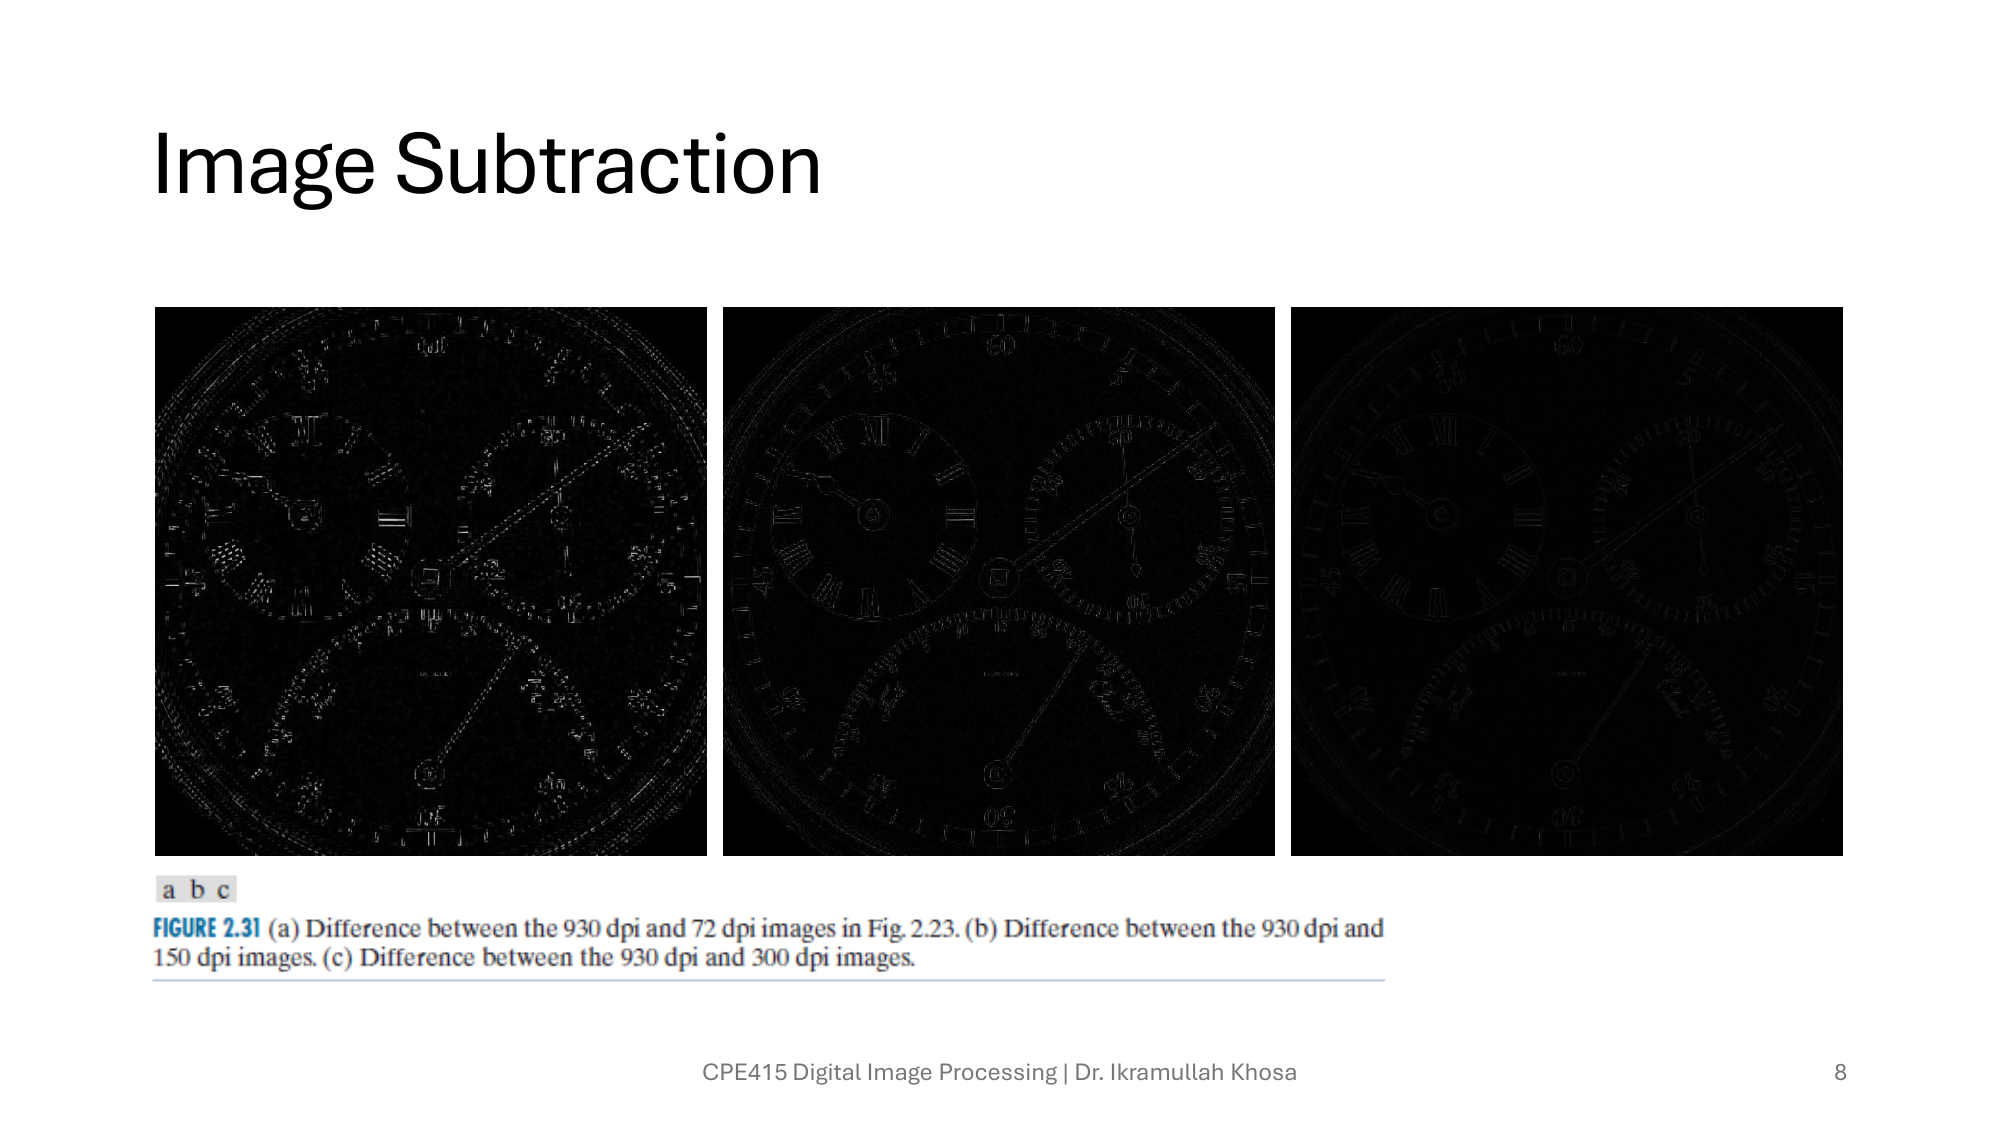
\includegraphics[width=0.85\textwidth]{images/slide4-08.png}
    \caption{Image arithmetic operations}
    \label{fig:arithmetic}
\end{figure}

\begin{deepexplanation}
\textbf{DEEP ANALYSIS - Figure \ref{fig:arithmetic}: Pixel-Wise Operations}

\textbf{The Basic Operations:}

\textbf{1. Addition:}
\[
g(x, y) = f_1(x, y) + f_2(x, y)
\]
\begin{itemize}
    \item Used for: Image averaging, combining images
    \item Caution: May exceed maximum value (overflow)
    \item Solution: Clip to max, or scale appropriately
\end{itemize}

\textbf{2. Subtraction:}
\[
g(x, y) = f_1(x, y) - f_2(x, y)
\]
\begin{itemize}
    \item Used for: Change detection, background removal
    \item Caution: May produce negative values (underflow)
    \item Solution: Take absolute value, or add offset
\end{itemize}

\textbf{3. Multiplication:}
\[
g(x, y) = f_1(x, y) \times f_2(x, y)
\]
\begin{itemize}
    \item Used for: Masking, shading correction
    \item Often with normalization: $g = f_1 \times f_2 / 255$
\end{itemize}

\textbf{4. Division:}
\[
g(x, y) = f_1(x, y) / f_2(x, y)
\]
\begin{itemize}
    \item Used for: Ratio images, illumination correction
    \item Caution: Division by zero!
    \item Solution: Add small constant to denominator
\end{itemize}

\textbf{Handling Overflow/Underflow:}
\begin{itemize}
    \item \textbf{Clipping}: $g = \min(\max(g, 0), 255)$
    \item \textbf{Scaling}: $g = g \times 255 / g_{max}$
    \item \textbf{Modular}: $g = g \mod 256$ (wraps around)
\end{itemize}
\end{deepexplanation}

\subsection{Image Averaging for Noise Reduction}

\begin{figure}[H]
    \centering
    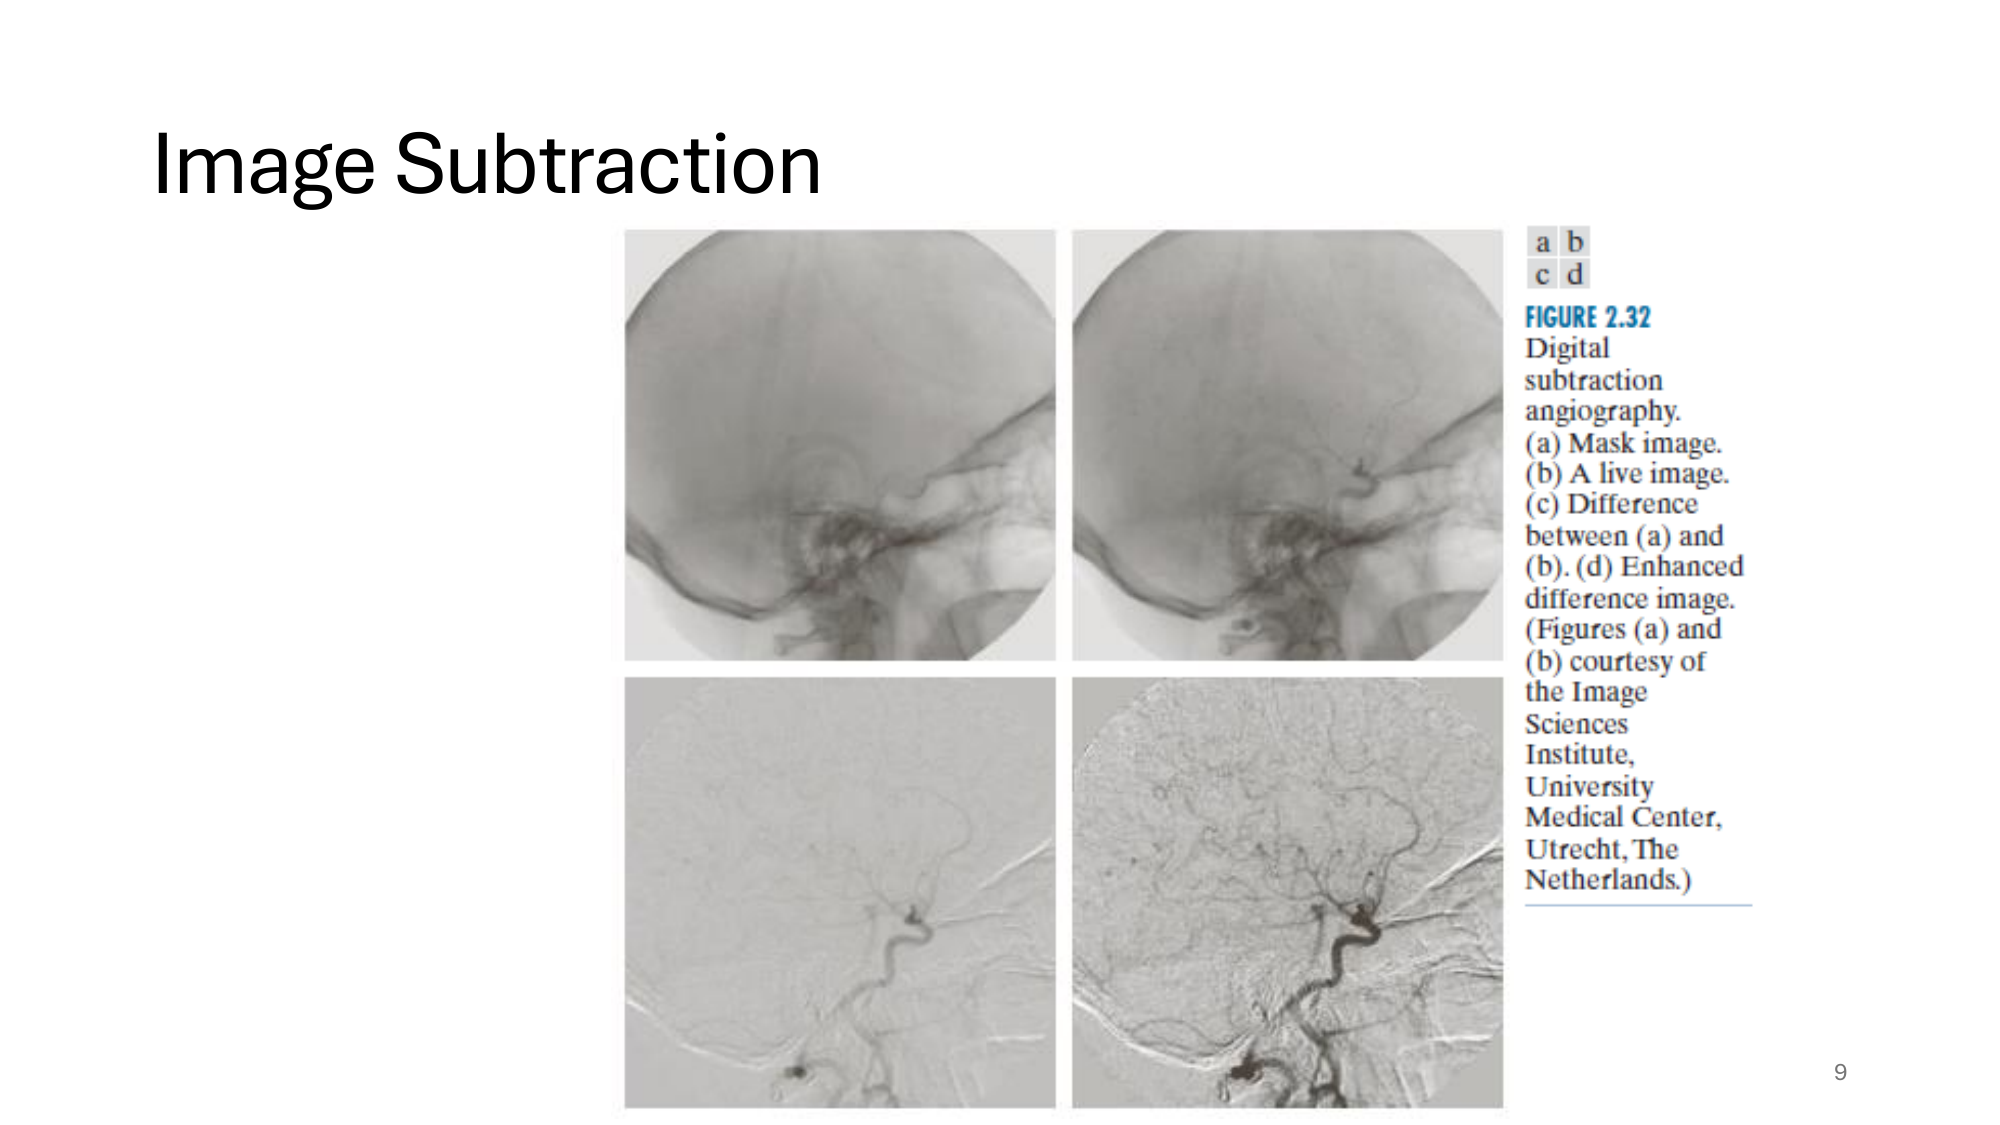
\includegraphics[width=0.9\textwidth]{images/slide4-09.png}
    \caption{Image averaging to reduce random noise}
    \label{fig:averaging}
\end{figure}

\begin{deepexplanation}
\textbf{DEEP ANALYSIS - Figure \ref{fig:averaging}: The Mathematics of Averaging}

\textbf{The Noise Model:}
Assume the observed image is:
\[
g(x, y) = f(x, y) + \eta(x, y)
\]
where $f$ = true image, $\eta$ = additive noise (zero-mean, random).

\textbf{The Averaging Process:}
Given $K$ noisy observations $g_1, g_2, \ldots, g_K$ of the same scene:
\[
\bar{g}(x, y) = \frac{1}{K} \sum_{i=1}^{K} g_i(x, y)
\]

\textbf{Why It Works:}
\begin{itemize}
    \item Signal $f(x, y)$: Same in every image $\rightarrow$ adds coherently
    \item Noise $\eta_i(x, y)$: Random, independent $\rightarrow$ partially cancels
\end{itemize}

\textbf{The Mathematics:}
Let noise variance in single image be $\sigma_\eta^2$.

After averaging $K$ images:
\[
\text{Var}(\bar{\eta}) = \frac{\sigma_\eta^2}{K}
\]
\[
\text{StdDev}(\bar{\eta}) = \frac{\sigma_\eta}{\sqrt{K}}
\]

\textbf{Signal-to-Noise Ratio Improvement:}
\[
\text{SNR improvement} = \sqrt{K}
\]
\begin{itemize}
    \item 4 images $\rightarrow$ 2× improvement
    \item 16 images $\rightarrow$ 4× improvement
    \item 100 images $\rightarrow$ 10× improvement
\end{itemize}

\textbf{Requirements:}
\begin{itemize}
    \item Multiple images of the \textbf{same} scene (no motion!)
    \item Noise must be \textbf{independent} between images
    \item Noise must be \textbf{zero-mean}
\end{itemize}
\end{deepexplanation}

\subsection{Image Subtraction}

\begin{figure}[H]
    \centering
    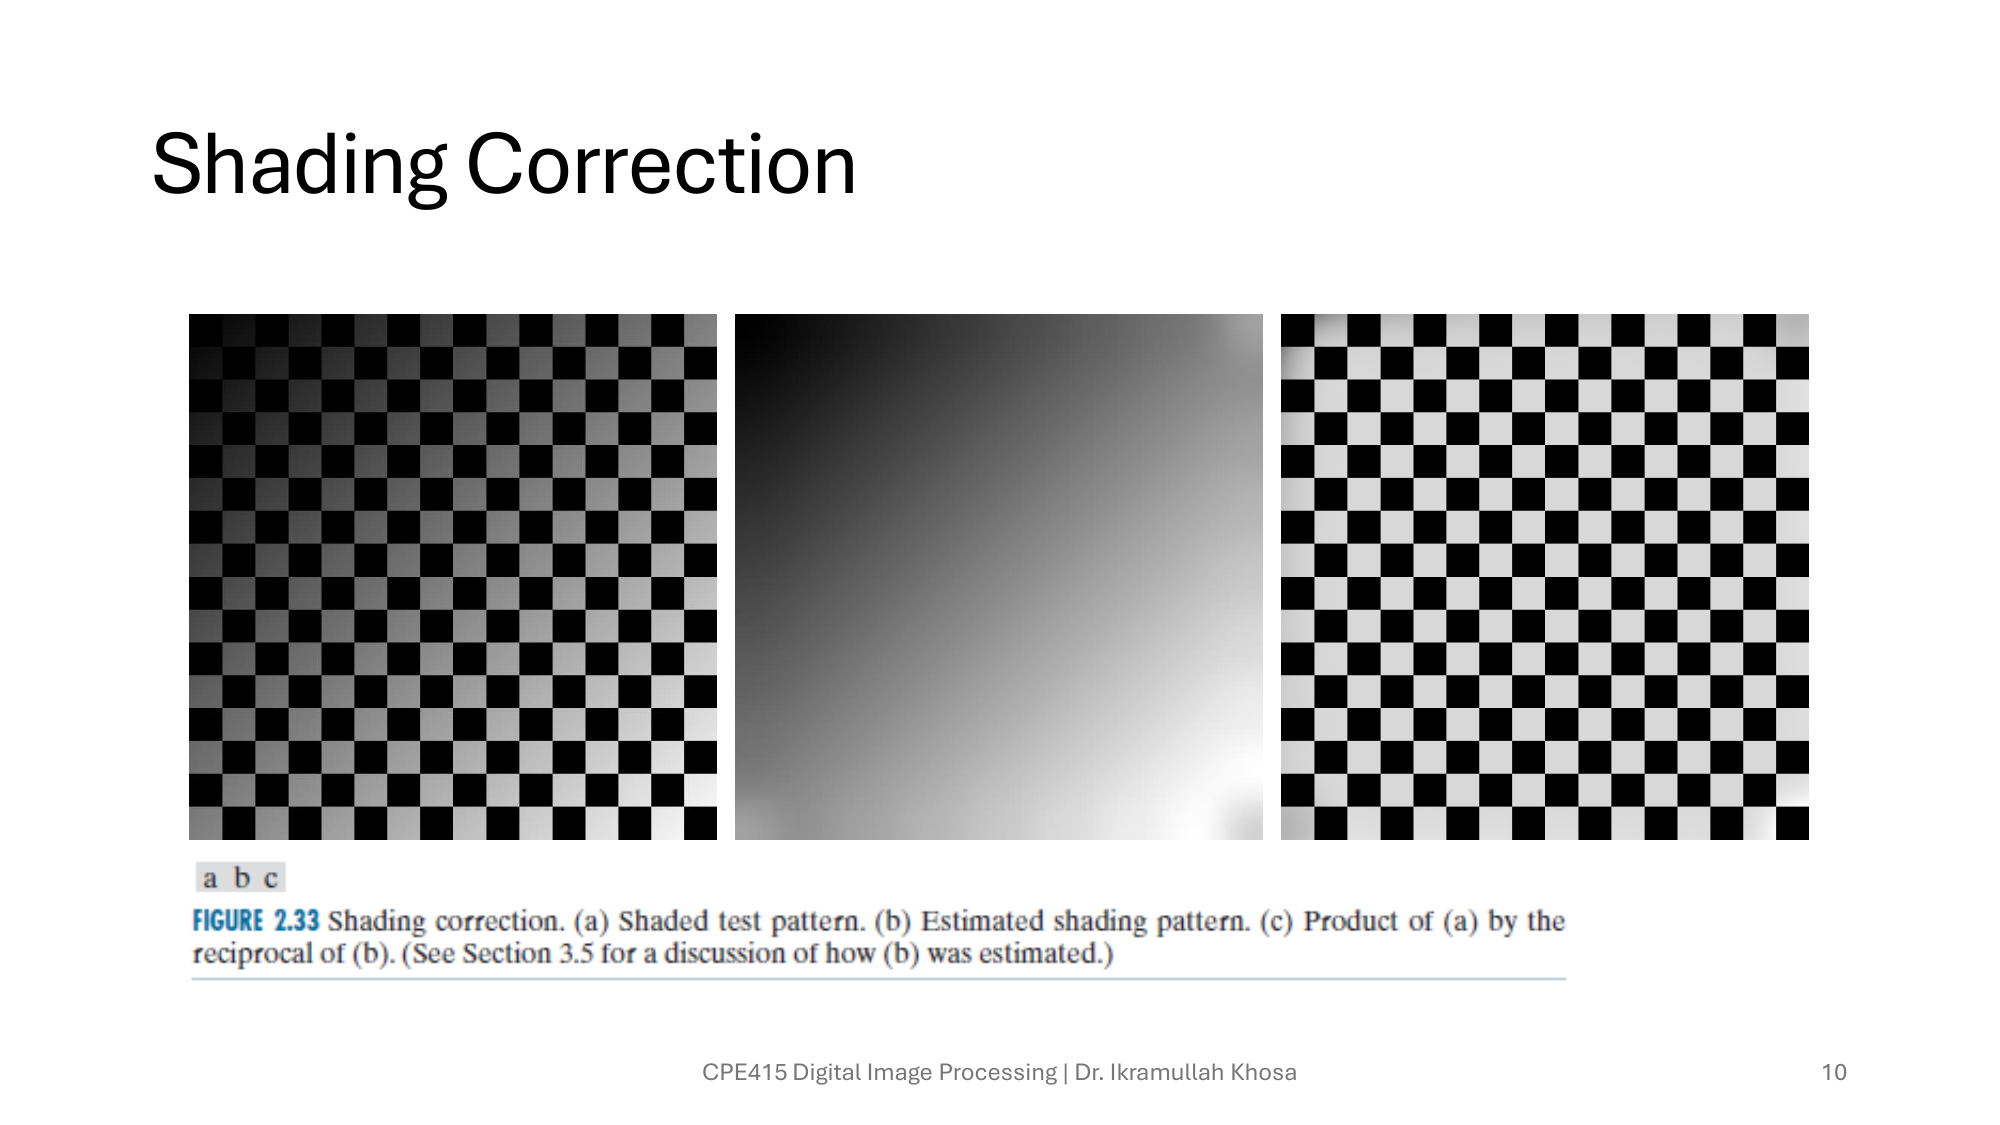
\includegraphics[width=0.9\textwidth]{images/slide4-10.png}
    \caption{Image subtraction for change detection}
    \label{fig:subtraction}
\end{figure}

\begin{deepexplanation}
\textbf{DEEP ANALYSIS - Figure \ref{fig:subtraction}: Difference Images}

\textbf{The Operation:}
\[
d(x, y) = f_1(x, y) - f_2(x, y)
\]

\textbf{Applications:}

\textbf{1. Change Detection:}
\begin{itemize}
    \item $f_1$ = current frame, $f_2$ = reference (background)
    \item $d(x, y) \neq 0$ indicates change/motion
    \item Threshold to get binary change mask
\end{itemize}

\textbf{2. Background Subtraction (Video):}
\begin{itemize}
    \item Maintain background model $B(x, y)$
    \item Foreground: $|f - B| > T$ (threshold)
    \item Commonly used in surveillance, traffic monitoring
\end{itemize}

\textbf{3. Medical Imaging (DSA --- Digital Subtraction Angiography):}
\begin{itemize}
    \item $f_1$ = image with contrast agent (blood vessels visible)
    \item $f_2$ = image without contrast (baseline)
    \item $d$ = only blood vessels visible (anatomy subtracted!)
\end{itemize}

\textbf{Practical Considerations:}
\begin{itemize}
    \item Results can be negative $\rightarrow$ use signed type or add offset
    \item Illumination changes cause false positives
    \item Registration must be precise
    \item Noise appears in difference image (adds in quadrature)
\end{itemize}

\textbf{Noise Behavior:}
If $f_1$ and $f_2$ have independent noise with variance $\sigma^2$:
\[
\text{Var}(d) = 2\sigma^2
\]
Difference images are \textbf{noisier} than originals!
\end{deepexplanation}

\subsection{Shading Correction}

\begin{figure}[H]
    \centering
    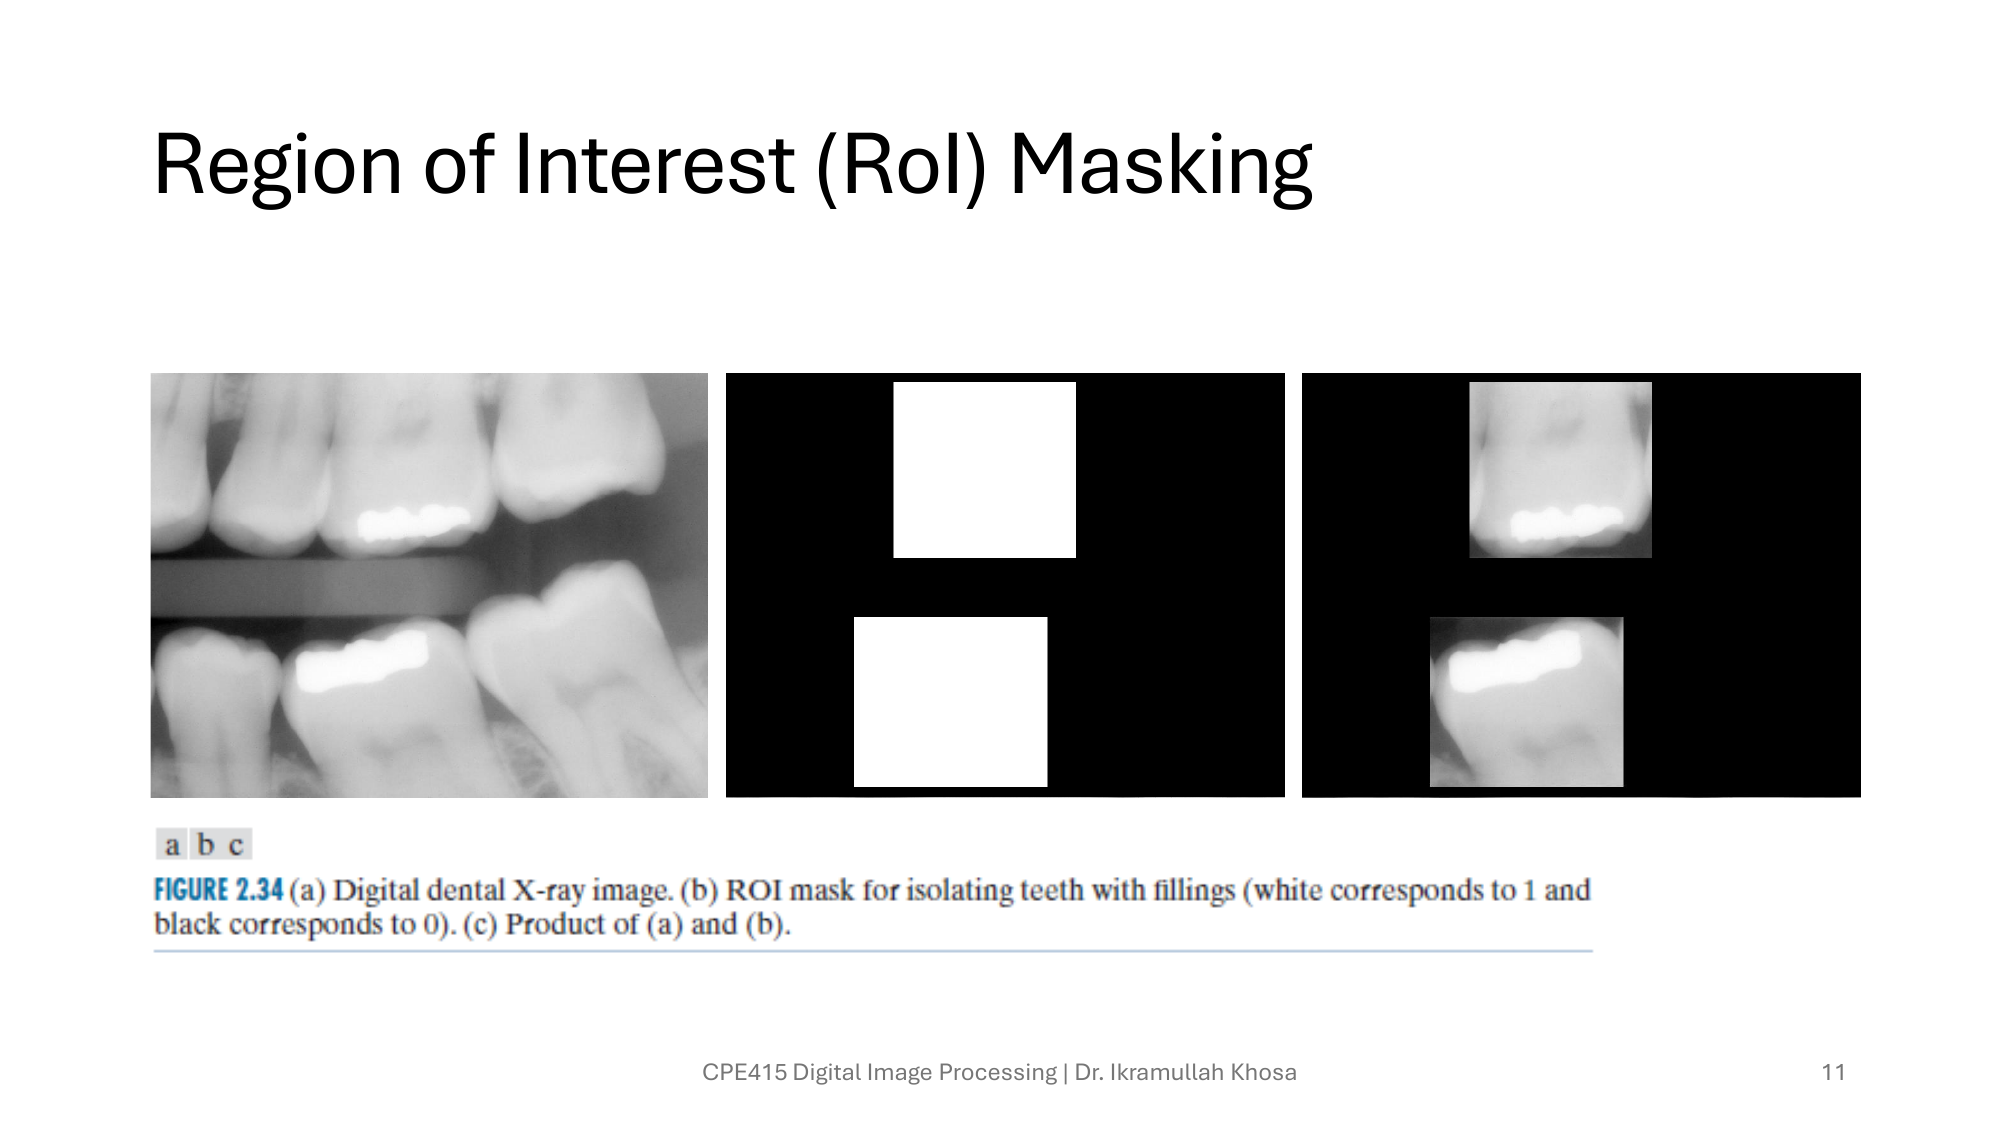
\includegraphics[width=0.85\textwidth]{images/slide4-11.png}
    \caption{Shading correction using division}
    \label{fig:shading}
\end{figure}

\begin{deepexplanation}
\textbf{DEEP ANALYSIS - Figure \ref{fig:shading}: Correcting Non-Uniform Illumination}

\textbf{The Problem:}
Images often have non-uniform brightness due to:
\begin{itemize}
    \item Uneven illumination
    \item Lens vignetting (darker corners)
    \item Sensor non-uniformity
\end{itemize}

\textbf{The Model:}
\[
f(x, y) = r(x, y) \cdot i(x, y)
\]
where $r$ = reflectance (what we want), $i$ = illumination (unwanted variation).

\textbf{The Solution --- Flat-Field Correction:}
\begin{enumerate}
    \item Capture a ``flat field'' image $i_{ref}(x, y)$:
    \begin{itemize}
        \item Image of uniform white surface
        \item Shows only illumination pattern
    \end{itemize}
    \item Correct the image:
    \[
    r(x, y) = \frac{f(x, y)}{i_{ref}(x, y)} \times C
    \]
    where $C$ is a normalization constant.
\end{enumerate}

\textbf{Practical Implementation:}
\begin{enumerate}
    \item Image a uniformly white/gray target $\rightarrow$ get $i_{ref}$
    \item For each pixel: $\text{corrected} = \text{original} \times \frac{\text{mean}(i_{ref})}{i_{ref}(x,y)}$
\end{enumerate}

\textbf{Alternative --- Polynomial Fitting:}
\begin{itemize}
    \item Fit low-order polynomial to background
    \item Subtract polynomial from image
    \item Works without reference image if background is smooth
\end{itemize}

\textbf{Common in:}
\begin{itemize}
    \item Microscopy (correct for uneven illumination)
    \item Photography (lens vignetting correction)
    \item Satellite imaging (sensor calibration)
\end{itemize}
\end{deepexplanation}

\subsection{Masking and ROI Operations}

\begin{figure}[H]
    \centering
    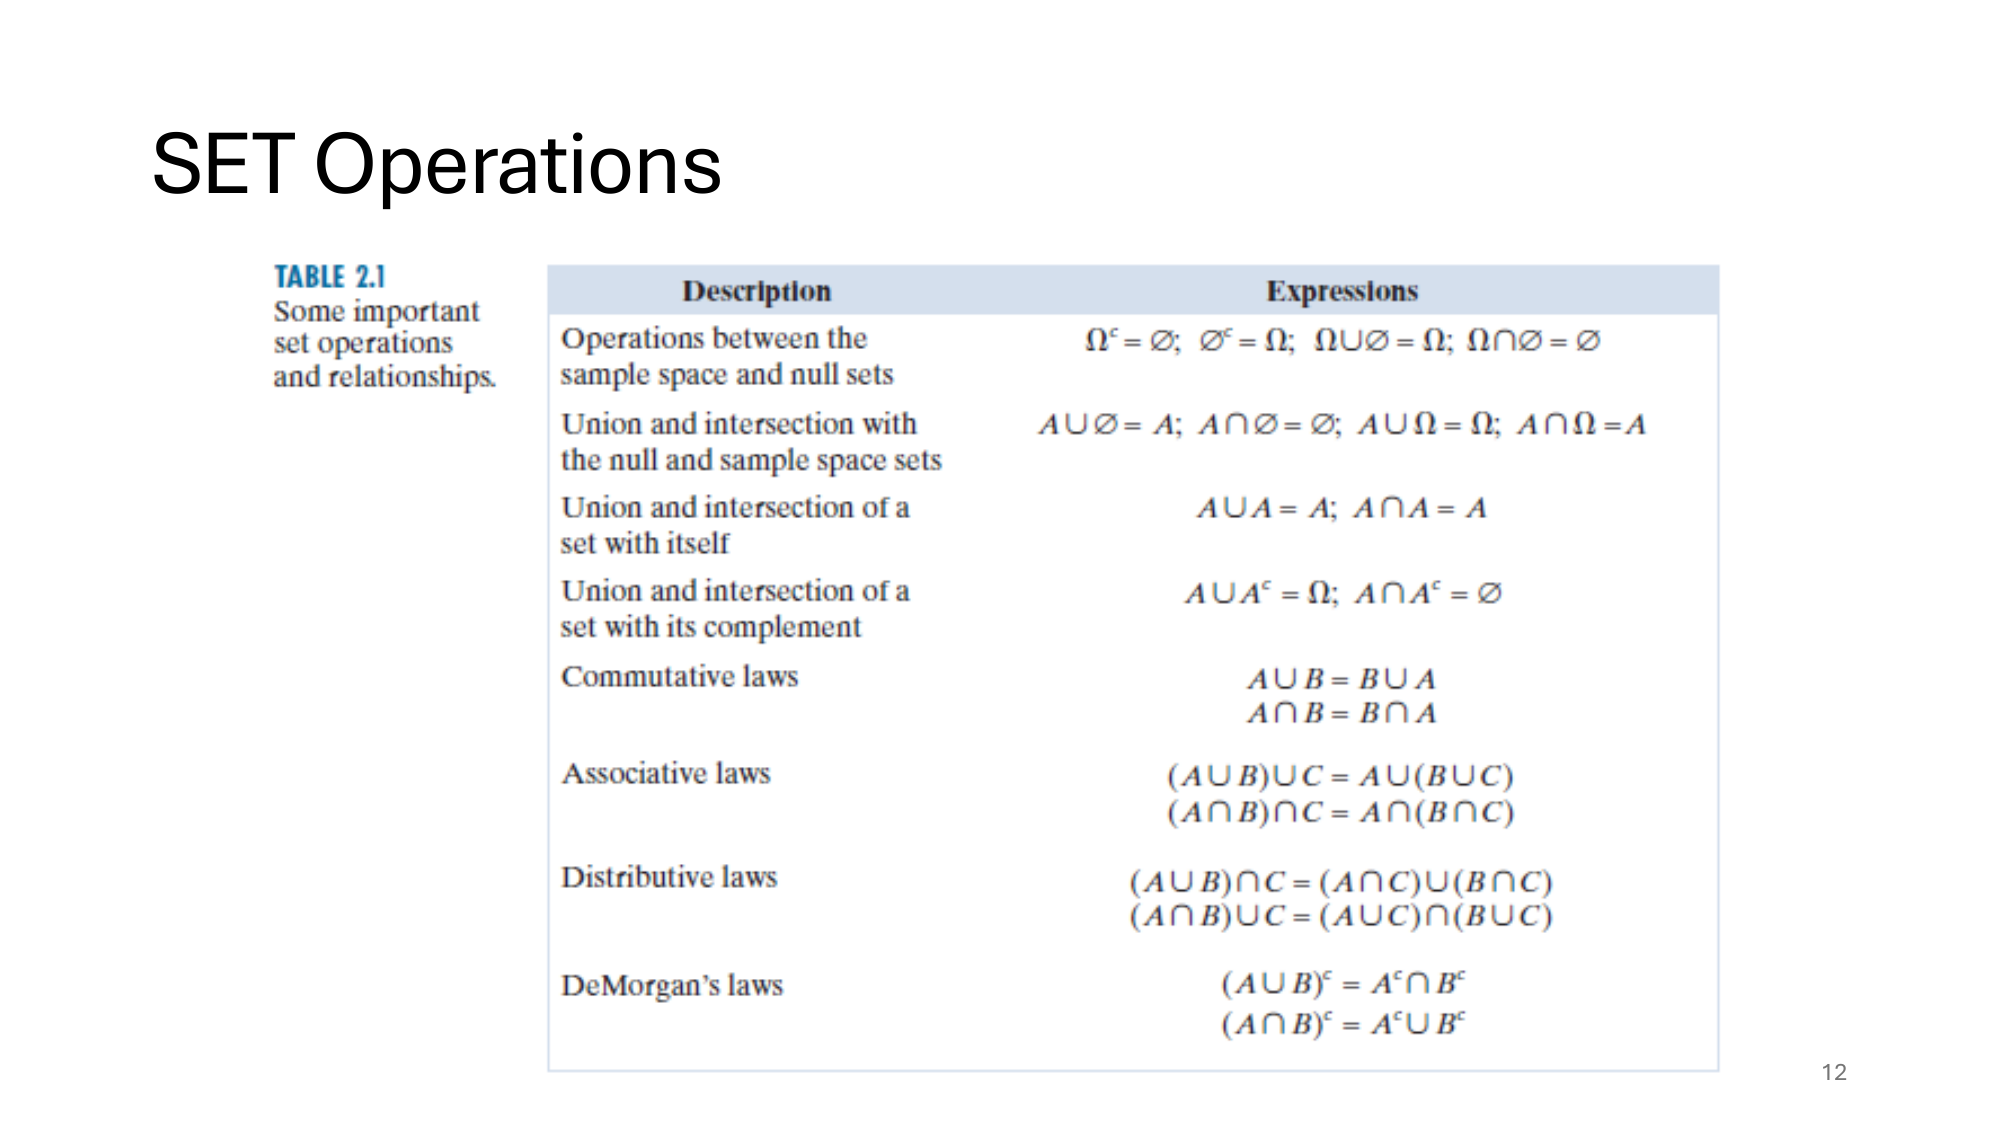
\includegraphics[width=0.85\textwidth]{images/slide4-12.png}
    \caption{Region of interest masking}
    \label{fig:masking}
\end{figure}

\begin{deepexplanation}
\textbf{DEEP ANALYSIS - Figure \ref{fig:masking}: Selective Processing with Masks}

\textbf{What Is a Mask?}
A binary image $M(x, y)$ where:
\begin{itemize}
    \item $M(x, y) = 1$ for pixels in the Region of Interest (ROI)
    \item $M(x, y) = 0$ for pixels outside the ROI
\end{itemize}

\textbf{Applying a Mask:}
\[
g(x, y) = f(x, y) \times M(x, y)
\]
\begin{itemize}
    \item ROI pixels: Preserved ($f \times 1 = f$)
    \item Background pixels: Set to zero ($f \times 0 = 0$)
\end{itemize}

\textbf{Common Mask Shapes:}
\begin{itemize}
    \item Rectangular (simple, axis-aligned)
    \item Circular (centered at point, specified radius)
    \item Polygonal (arbitrary shape)
    \item Arbitrary (from segmentation, user drawing)
\end{itemize}

\textbf{Operations with Masks:}
\begin{itemize}
    \item \textbf{Extract}: Get only ROI pixels
    \item \textbf{Replace}: Put processed ROI back into original
    \item \textbf{Statistics}: Compute mean, variance only in ROI
    \item \textbf{Selective processing}: Apply filter only to ROI
\end{itemize}

\textbf{Alternative Formulation:}
To blend/composite:
\[
g = M \cdot f_1 + (1 - M) \cdot f_2
\]
Puts $f_1$ in ROI, $f_2$ elsewhere (feathered edges if $M$ has intermediate values).
\end{deepexplanation}


\subsection{Set Operations on Images}

\begin{figure}[H]
    \centering
    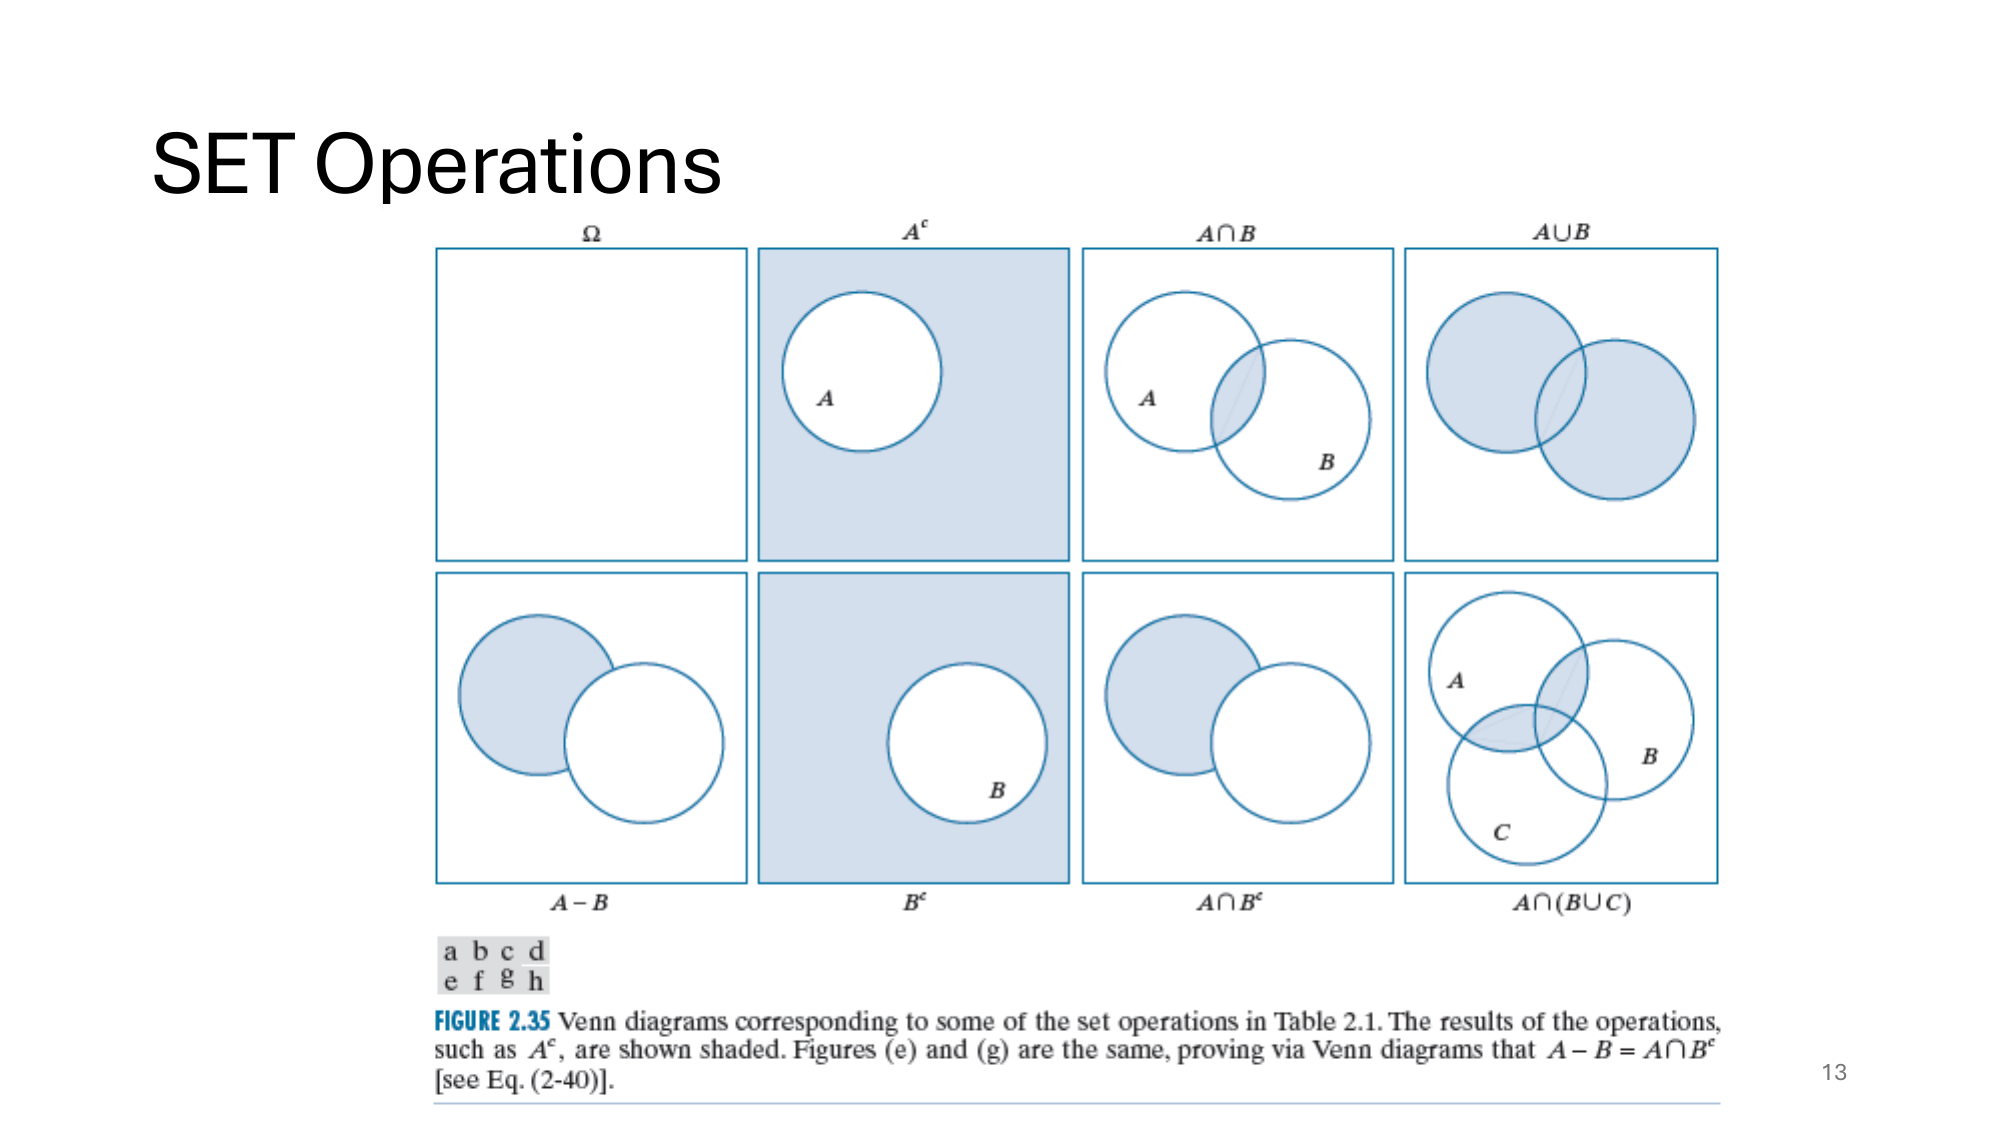
\includegraphics[width=0.85\textwidth]{images/slide4-13.png}
    \caption{Set operations: union, intersection, complement}
    \label{fig:set_operations}
\end{figure}

\begin{deepexplanation}
\textbf{DEEP ANALYSIS - Figure \ref{fig:set_operations}: Logical Operations on Binary Images}

\textbf{Binary Images as Sets:}
In a binary image, foreground pixels form a set $A$:
\[
A = \{(x, y) : f(x, y) = 1\}
\]

\textbf{Set Operations:}

\textbf{1. Complement (NOT):}
\[
A^c = \{(x, y) : f(x, y) = 0\} = \text{background}
\]
\begin{itemize}
    \item Swaps foreground and background
    \item $f^c(x, y) = 1 - f(x, y)$ (or $255 - f$ for grayscale)
\end{itemize}

\textbf{2. Union (OR):}
\[
A \cup B = \{(x, y) : f_A(x, y) = 1 \text{ OR } f_B(x, y) = 1\}
\]
\begin{itemize}
    \item Combines foregrounds from both images
    \item Pixel is 1 if it's 1 in either image
    \item $g(x, y) = \max(f_A(x, y), f_B(x, y))$
\end{itemize}

\textbf{3. Intersection (AND):}
\[
A \cap B = \{(x, y) : f_A(x, y) = 1 \text{ AND } f_B(x, y) = 1\}
\]
\begin{itemize}
    \item Keeps only pixels that are 1 in both images
    \item $g(x, y) = \min(f_A(x, y), f_B(x, y))$
\end{itemize}

\textbf{4. Difference (A but not B):}
\[
A - B = A \cap B^c = \{(x, y) : f_A = 1 \text{ AND } f_B = 0\}
\]
\begin{itemize}
    \item Pixels in $A$ that are not in $B$
    \item $g = f_A \cdot (1 - f_B)$
\end{itemize}

\textbf{Applications:}
\begin{itemize}
    \item Combining multiple segmentation results
    \item Removing regions (set difference)
    \item Finding overlap between regions
    \item Morphological operations build on these
\end{itemize}
\end{deepexplanation}

\begin{figure}[H]
    \centering
    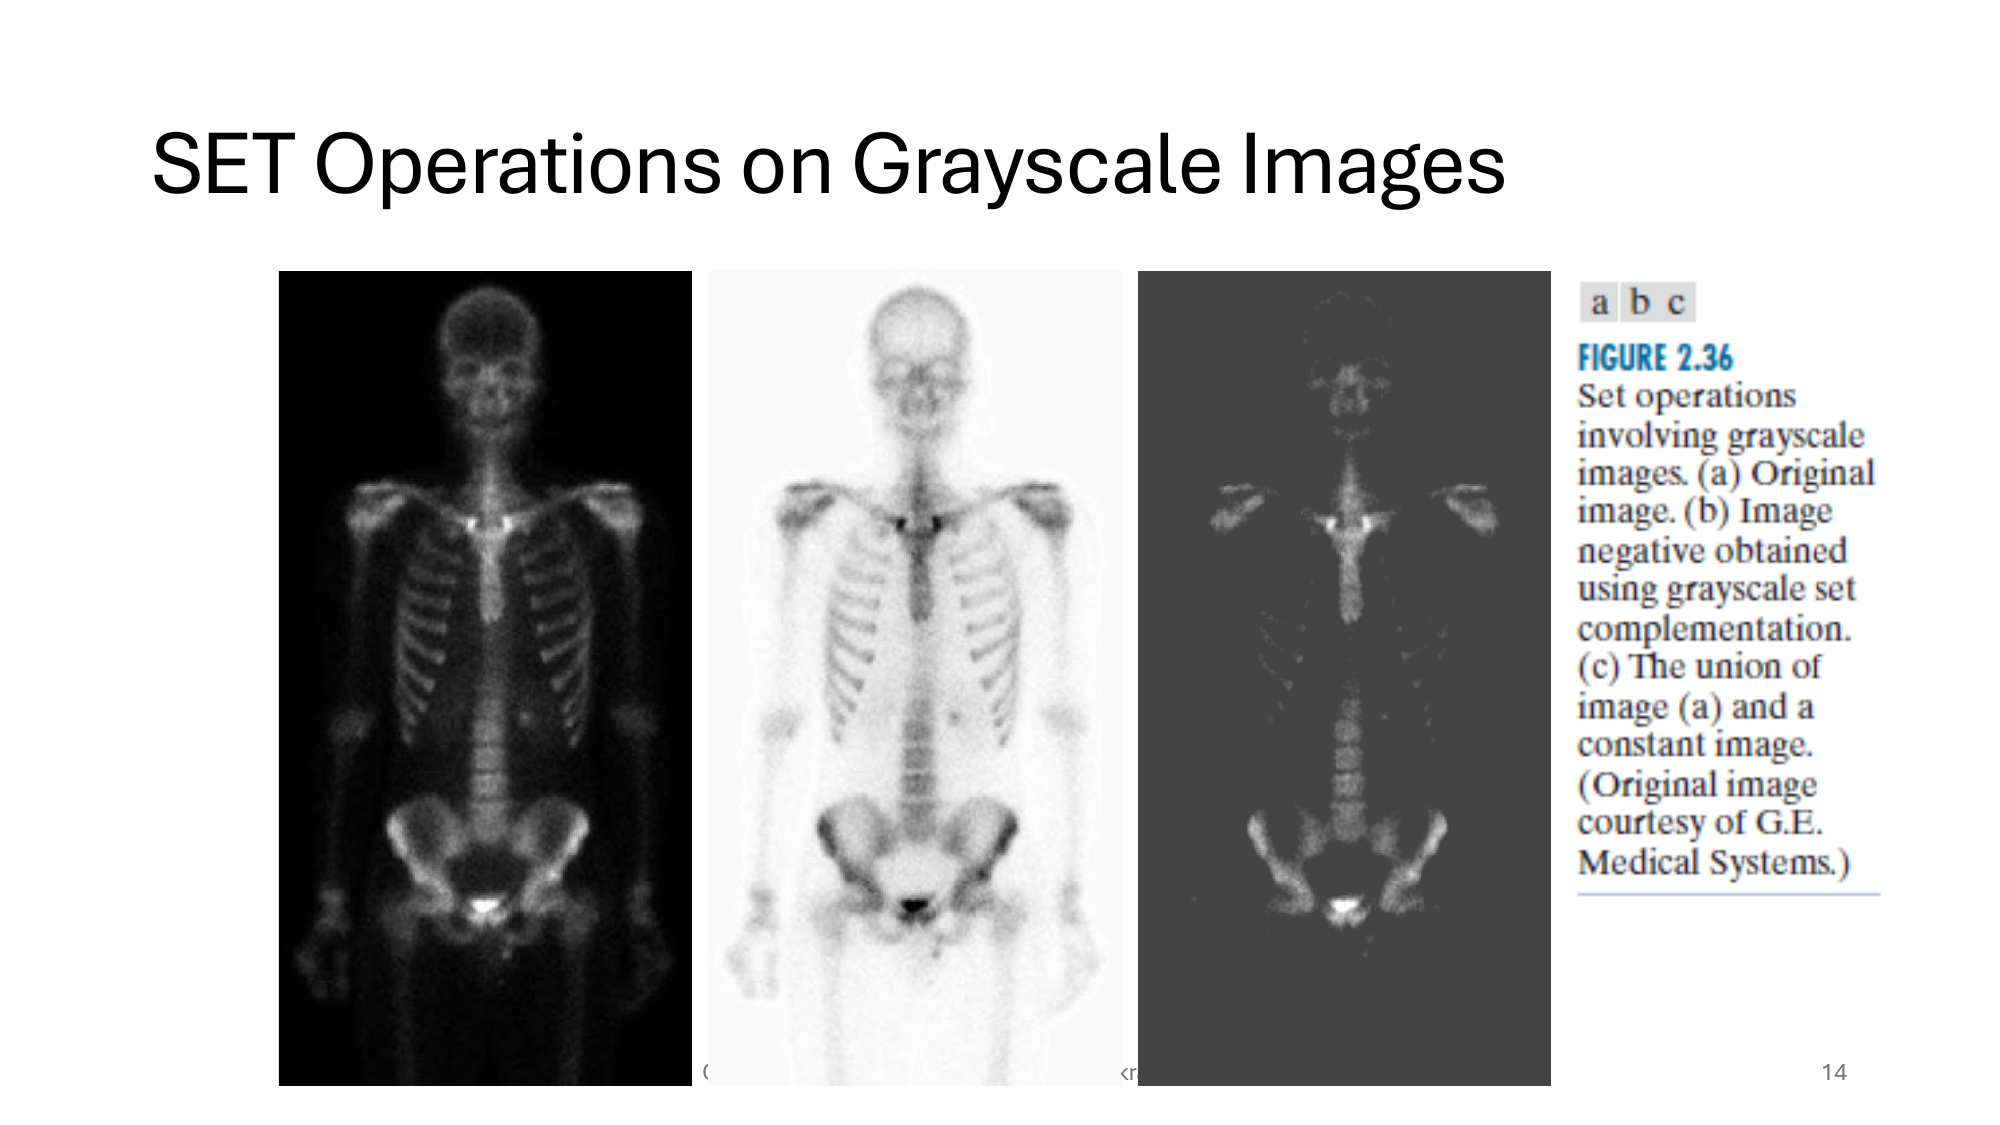
\includegraphics[width=0.85\textwidth]{images/slide4-14.png}
    \caption{Set difference and symmetric difference}
    \label{fig:set_diff}
\end{figure}

%==============================================================================
\section{Geometric Transformations}
%==============================================================================

\subsection{Basic Spatial Transformations}

\begin{figure}[H]
    \centering
    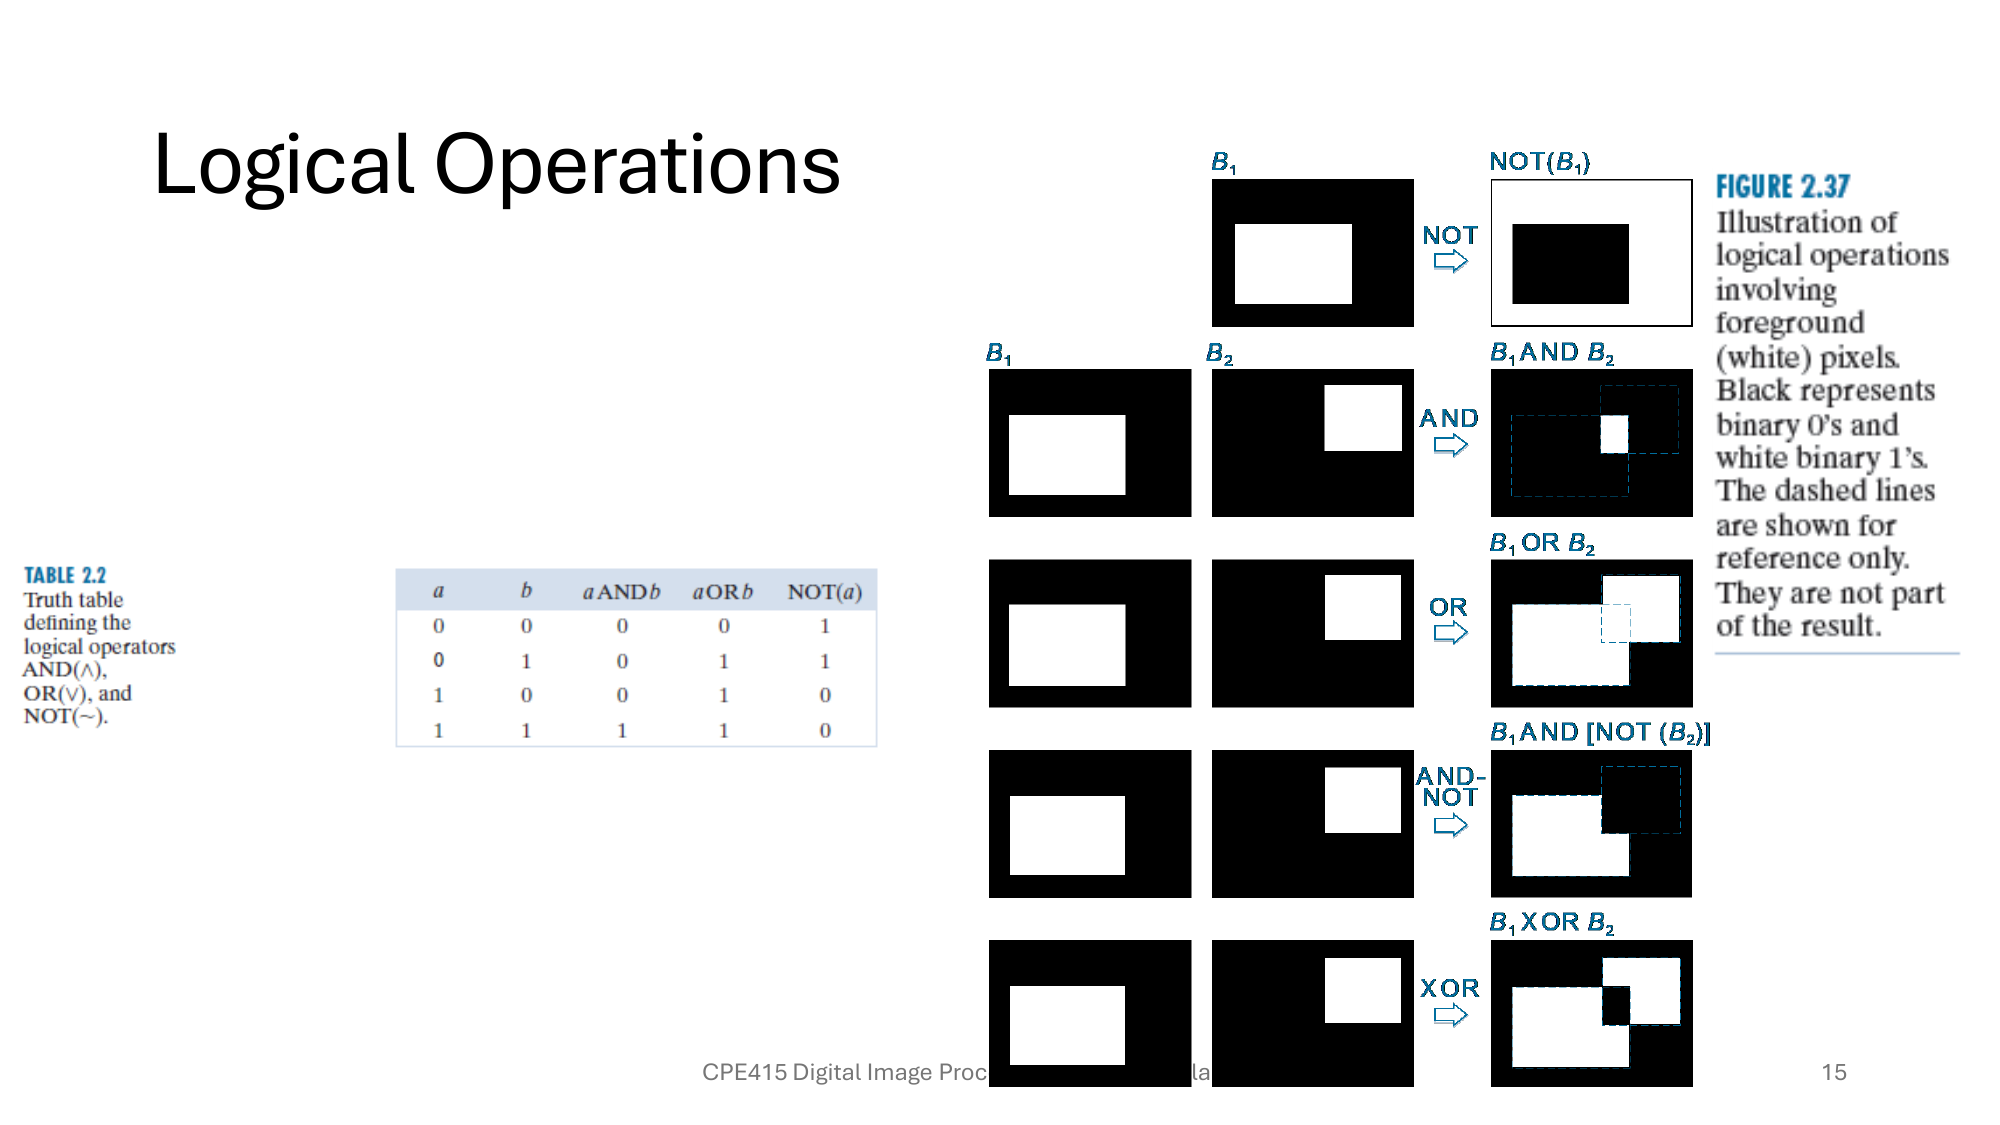
\includegraphics[width=0.9\textwidth]{images/slide4-15.png}
    \caption{Basic geometric transformations: translation, rotation, scaling}
    \label{fig:geometric_transforms}
\end{figure}

\begin{deepexplanation}
\textbf{DEEP ANALYSIS - Figure \ref{fig:geometric_transforms}: Coordinate Transformations}

\textbf{General Form:}
A geometric transformation maps input coordinates $(x, y)$ to output coordinates $(x', y')$:
\[
(x', y') = T(x, y)
\]

\textbf{1. Translation (Shift):}
\[
x' = x + t_x, \quad y' = y + t_y
\]
\begin{itemize}
    \item Moves image by $(t_x, t_y)$
    \item Shape and size unchanged
\end{itemize}

\textbf{2. Scaling:}
\[
x' = s_x \cdot x, \quad y' = s_y \cdot y
\]
\begin{itemize}
    \item $s > 1$: Enlargement
    \item $s < 1$: Shrinking
    \item $s_x \neq s_y$: Non-uniform (stretching)
\end{itemize}

\textbf{3. Rotation (about origin):}
\[
x' = x\cos\theta - y\sin\theta
\]
\[
y' = x\sin\theta + y\cos\theta
\]
\begin{itemize}
    \item Rotates by angle $\theta$ counterclockwise
    \item Preserves shape and size
\end{itemize}

\textbf{4. Shear:}
\[
x' = x + sh_x \cdot y, \quad y' = y + sh_y \cdot x
\]
\begin{itemize}
    \item ``Slants'' the image
    \item Vertical lines become diagonal
\end{itemize}

\textbf{Homogeneous Coordinates:}
All these can be written as $3 \times 3$ matrix:
\[
\begin{bmatrix} x' \\ y' \\ 1 \end{bmatrix} = 
\begin{bmatrix} a & b & c \\ d & e & f \\ 0 & 0 & 1 \end{bmatrix}
\begin{bmatrix} x \\ y \\ 1 \end{bmatrix}
\]

This allows \textbf{composing} transformations by matrix multiplication!
\end{deepexplanation}

\begin{figure}[H]
    \centering
    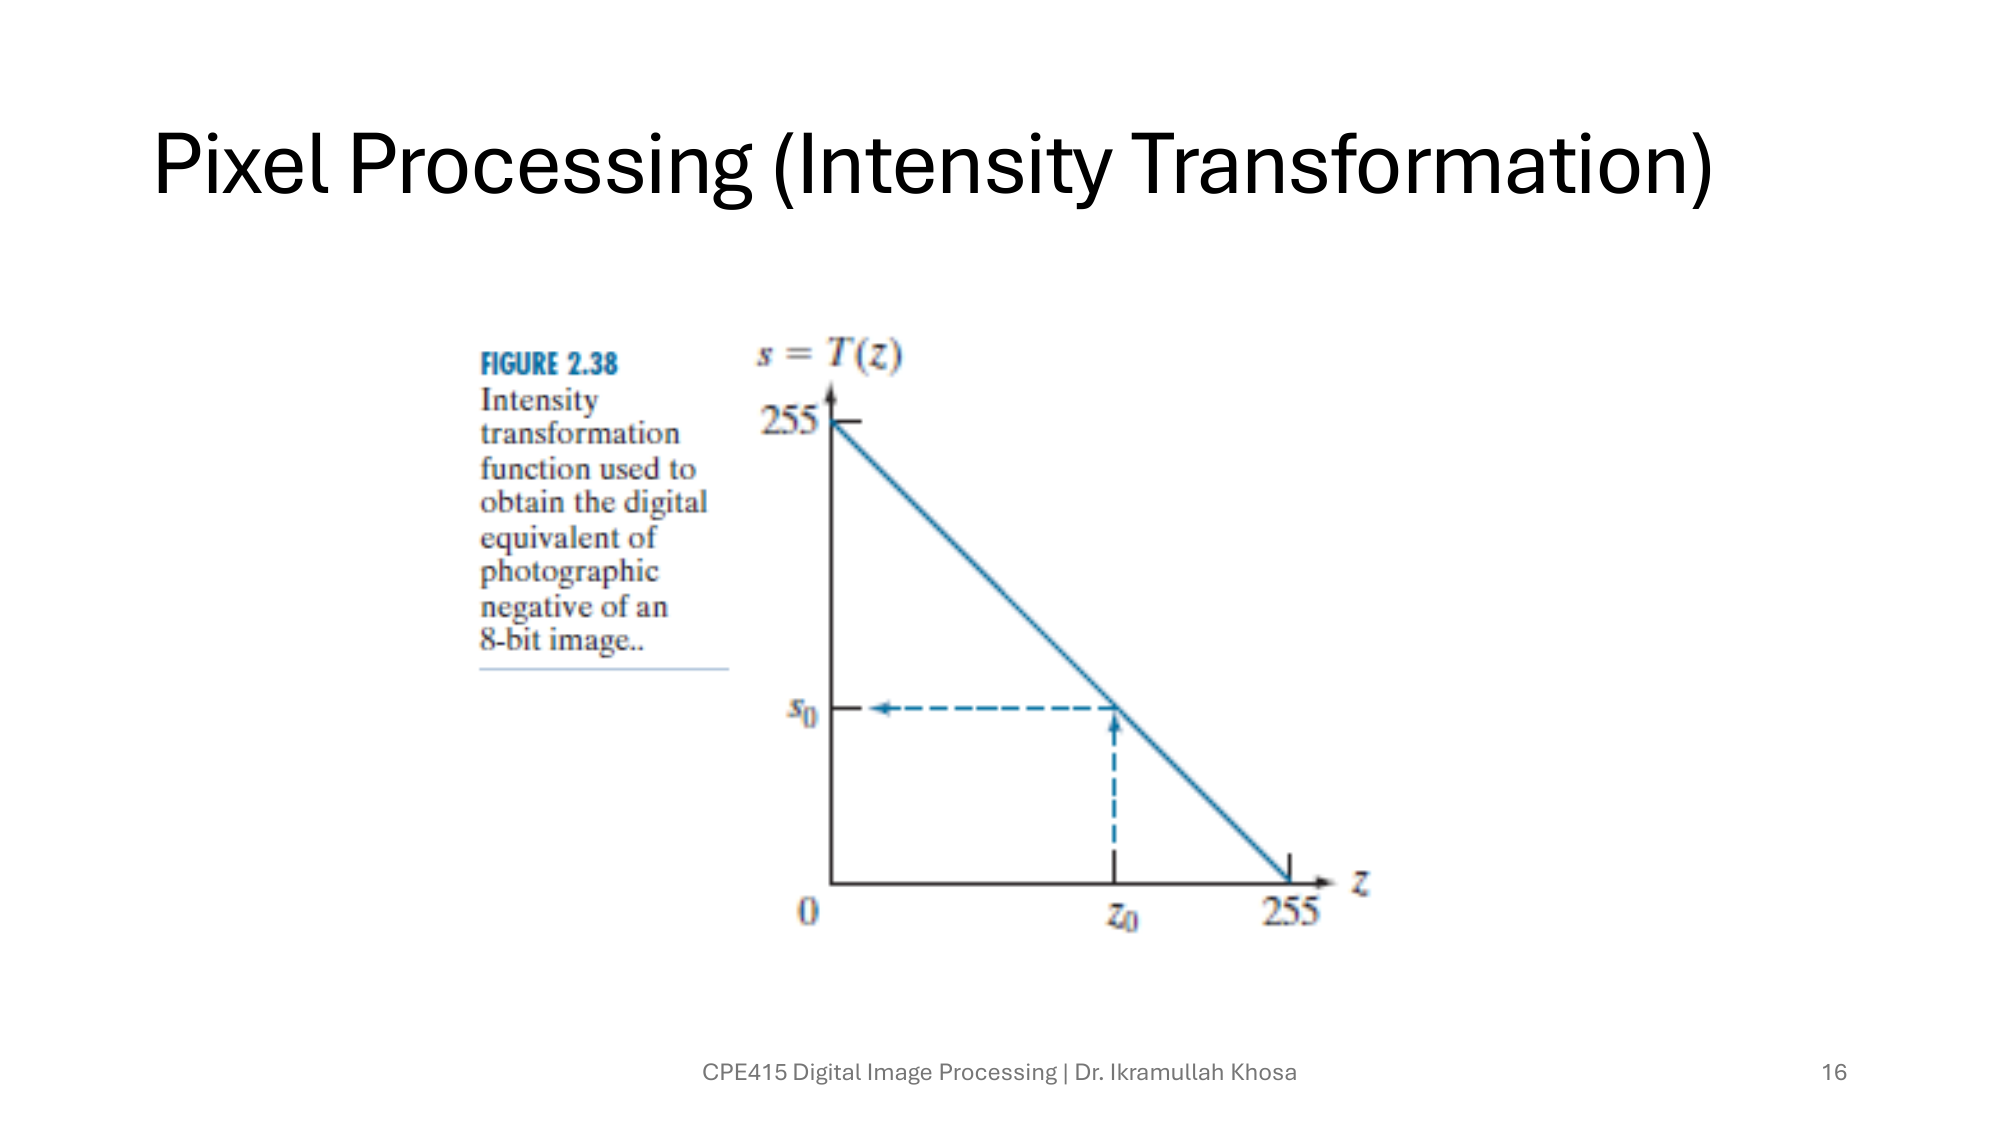
\includegraphics[width=0.85\textwidth]{images/slide4-16.png}
    \caption{Affine transformation matrix}
    \label{fig:affine}
\end{figure}

\begin{deepexplanation}
\textbf{DEEP ANALYSIS - Figure \ref{fig:affine}: Affine Transformations}

\textbf{The General Affine Transformation:}
\[
\begin{bmatrix} x' \\ y' \end{bmatrix} = 
\begin{bmatrix} a_{11} & a_{12} \\ a_{21} & a_{22} \end{bmatrix}
\begin{bmatrix} x \\ y \end{bmatrix} +
\begin{bmatrix} b_1 \\ b_2 \end{bmatrix}
\]

Or in homogeneous coordinates:
\[
\begin{bmatrix} x' \\ y' \\ 1 \end{bmatrix} = 
\begin{bmatrix} a_{11} & a_{12} & b_1 \\ a_{21} & a_{22} & b_2 \\ 0 & 0 & 1 \end{bmatrix}
\begin{bmatrix} x \\ y \\ 1 \end{bmatrix}
\]

\textbf{Properties of Affine Transformations:}
\begin{itemize}
    \item Lines remain lines (straight lines stay straight)
    \item Parallel lines remain parallel
    \item Ratios of distances along lines are preserved
    \item Areas are scaled uniformly
\end{itemize}

\textbf{What Is NOT Preserved:}
\begin{itemize}
    \item Angles (in general)
    \item Lengths (unless pure rotation/translation)
    \item Circular shapes (become ellipses under general affine)
\end{itemize}

\textbf{Degrees of Freedom:}
\begin{itemize}
    \item 6 parameters: $a_{11}, a_{12}, a_{21}, a_{22}, b_1, b_2$
    \item Need 3 point correspondences to determine transformation
    \item Each point gives 2 equations $(x', y')$
\end{itemize}

\textbf{Finding Affine Parameters:}
Given 3 corresponding point pairs $(x_i, y_i) \leftrightarrow (x'_i, y'_i)$:

Solve the system:
\[
\begin{bmatrix} 
x_1 & y_1 & 1 & 0 & 0 & 0 \\
0 & 0 & 0 & x_1 & y_1 & 1 \\
x_2 & y_2 & 1 & 0 & 0 & 0 \\
0 & 0 & 0 & x_2 & y_2 & 1 \\
x_3 & y_3 & 1 & 0 & 0 & 0 \\
0 & 0 & 0 & x_3 & y_3 & 1 \\
\end{bmatrix}
\begin{bmatrix} a_{11} \\ a_{12} \\ b_1 \\ a_{21} \\ a_{22} \\ b_2 \end{bmatrix} = 
\begin{bmatrix} x'_1 \\ y'_1 \\ x'_2 \\ y'_2 \\ x'_3 \\ y'_3 \end{bmatrix}
\]
\end{deepexplanation}

\subsection{Image Registration}

\begin{figure}[H]
    \centering
    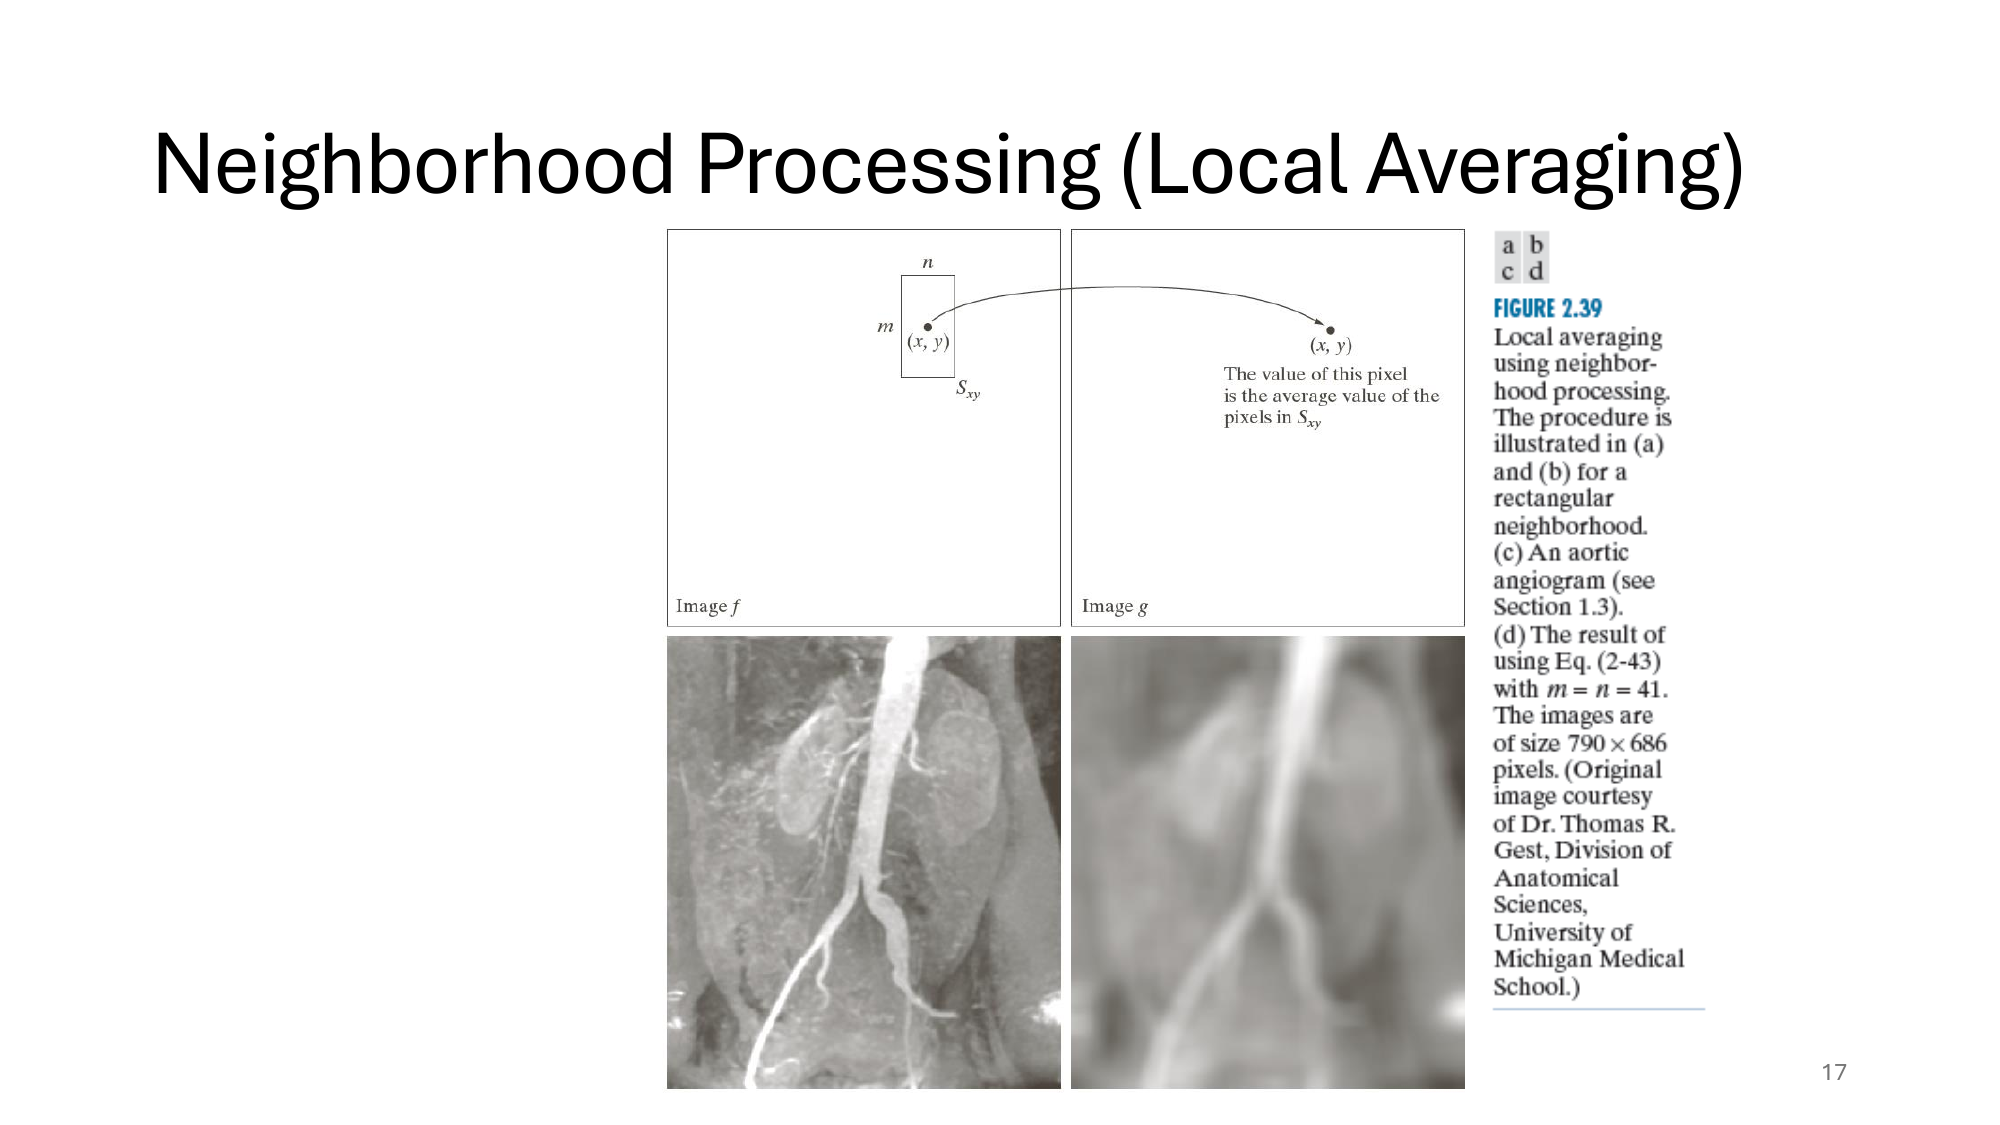
\includegraphics[width=0.9\textwidth]{images/slide4-17.png}
    \caption{Image registration: aligning two images}
    \label{fig:registration}
\end{figure}

\begin{deepexplanation}
\textbf{DEEP ANALYSIS - Figure \ref{fig:registration}: Aligning Images}

\textbf{What Is Image Registration?}
The process of transforming one image to align with another:
\begin{itemize}
    \item Same scene, different viewpoints
    \item Same scene, different times
    \item Different modalities (MRI and CT)
\end{itemize}

\textbf{The Process:}
\begin{enumerate}
    \item \textbf{Feature Detection}: Find distinctive points in both images
    \begin{itemize}
        \item Corners (Harris, FAST)
        \item Blobs (SIFT, SURF)
        \item Manual selection (control points)
    \end{itemize}
    
    \item \textbf{Feature Matching}: Find corresponding points
    \begin{itemize}
        \item Based on local appearance
        \item RANSAC for outlier rejection
    \end{itemize}
    
    \item \textbf{Transformation Estimation}: Compute best-fit transformation
    \begin{itemize}
        \item Least squares if more than minimum points
        \item Type depends on expected distortion (affine, projective, etc.)
    \end{itemize}
    
    \item \textbf{Resampling}: Apply transformation and interpolate
    \begin{itemize}
        \item Forward mapping or inverse mapping
        \item Use bilinear/bicubic interpolation
    \end{itemize}
\end{enumerate}

\textbf{Forward vs. Inverse Mapping:}

\textbf{Forward Mapping:}
\begin{itemize}
    \item For each input pixel $(x, y)$, compute output $(x', y')$
    \item Problem: Output pixels may have holes or multiple values
\end{itemize}

\textbf{Inverse Mapping (Preferred):}
\begin{itemize}
    \item For each output pixel $(x', y')$, compute input $(x, y)$
    \item No holes; interpolate if $(x, y)$ is non-integer
\end{itemize}

\textbf{Applications:}
\begin{itemize}
    \item Medical imaging (aligning scans)
    \item Remote sensing (orthorectification)
    \item Panorama stitching
    \item Motion compensation in video
\end{itemize}
\end{deepexplanation}

\begin{figure}[H]
    \centering
    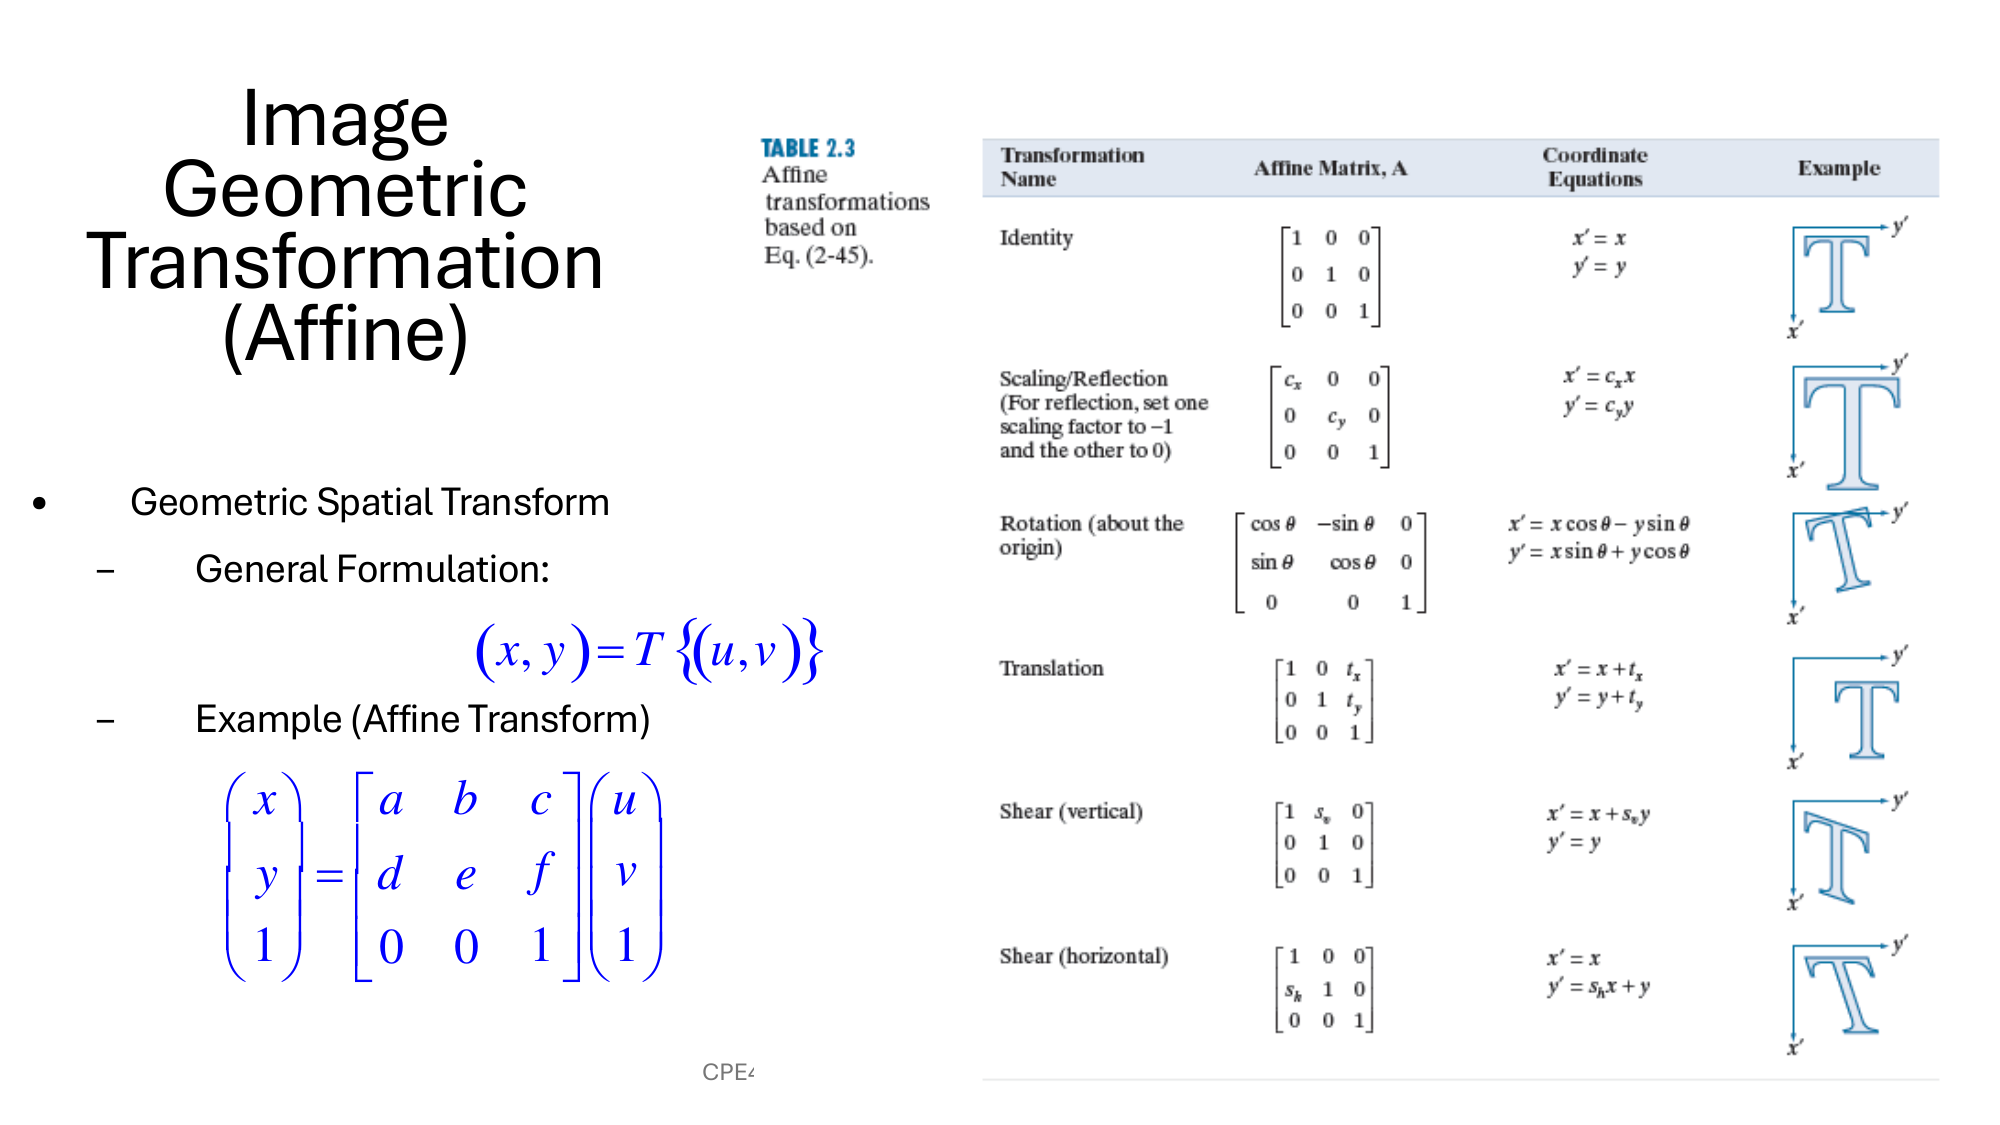
\includegraphics[width=0.85\textwidth]{images/slide4-18.png}
    \caption{Transformation types and their properties}
    \label{fig:transform_types}
\end{figure}

\begin{deepexplanation}
\textbf{DEEP ANALYSIS - Figure \ref{fig:transform_types}: Hierarchy of Transformations}

\textbf{From Most Restrictive to Most General:}

\textbf{1. Rigid (Euclidean) Transformation:}
\begin{itemize}
    \item Rotation + Translation only
    \item \textbf{Preserves}: Distances, angles, shapes
    \item Parameters: 3 (rotation angle, $t_x$, $t_y$)
    \item Minimum points: 2
\end{itemize}

\textbf{2. Similarity Transformation:}
\begin{itemize}
    \item Rotation + Translation + Uniform Scaling
    \item \textbf{Preserves}: Angles, shapes (not sizes)
    \item Parameters: 4 (rotation, scale, $t_x$, $t_y$)
    \item Minimum points: 2
\end{itemize}

\textbf{3. Affine Transformation:}
\begin{itemize}
    \item All linear transformations + translation
    \item \textbf{Preserves}: Parallelism, ratios of distances on lines
    \item Parameters: 6
    \item Minimum points: 3
\end{itemize}

\textbf{4. Projective (Perspective) Transformation:}
\begin{itemize}
    \item Models camera viewing geometry
    \item \textbf{Preserves}: Straight lines (only!)
    \item Parameters: 8
    \item Minimum points: 4
\end{itemize}

\textbf{5. Polynomial/Elastic:}
\begin{itemize}
    \item Non-linear, locally varying
    \item Can model lens distortion, tissue deformation
    \item Many parameters (depends on polynomial order)
\end{itemize}

\textbf{Choosing the Right Transformation:}
\begin{itemize}
    \item Scanned documents: Affine usually sufficient
    \item Photographs with perspective: Projective
    \item Medical images: Often elastic/non-rigid
    \item The simpler the model that fits, the more robust
\end{itemize}
\end{deepexplanation}

\begin{figure}[H]
    \centering
    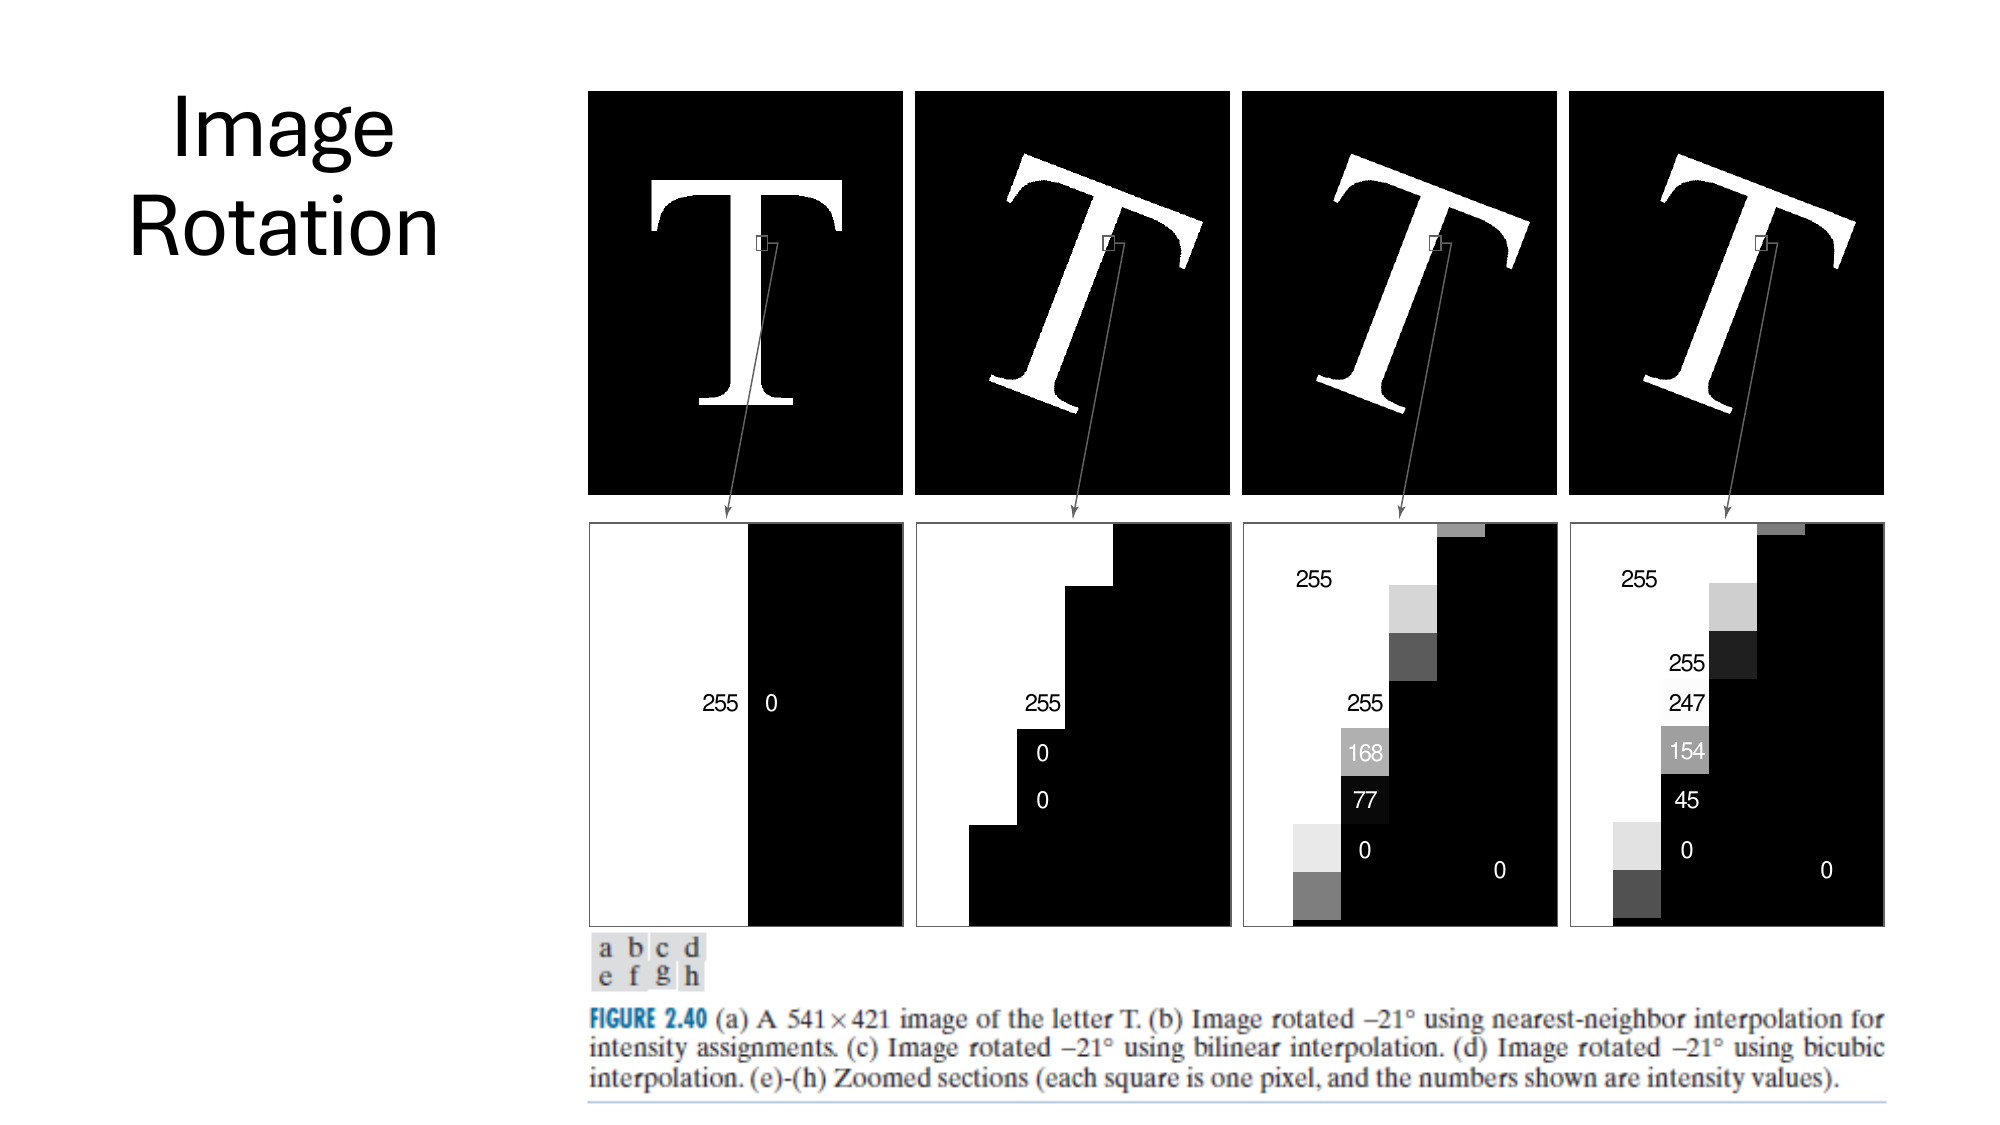
\includegraphics[width=0.85\textwidth]{images/slide4-19.png}
    \caption{Projective (perspective) transformation}
    \label{fig:projective}
\end{figure}

\begin{deepexplanation}
\textbf{DEEP ANALYSIS - Figure \ref{fig:projective}: Perspective Correction}

\textbf{The Projective Transformation:}
\[
x' = \frac{a_{11}x + a_{12}y + a_{13}}{a_{31}x + a_{32}y + 1}
\]
\[
y' = \frac{a_{21}x + a_{22}y + a_{23}}{a_{31}x + a_{32}y + 1}
\]

\textbf{In Homogeneous Coordinates:}
\[
\begin{bmatrix} x'' \\ y'' \\ w \end{bmatrix} = 
\begin{bmatrix} a_{11} & a_{12} & a_{13} \\ a_{21} & a_{22} & a_{23} \\ a_{31} & a_{32} & 1 \end{bmatrix}
\begin{bmatrix} x \\ y \\ 1 \end{bmatrix}
\]
Then: $x' = x''/w$, $y' = y''/w$

\textbf{What Projective Can Do That Affine Cannot:}
\begin{itemize}
    \item Model foreshortening (distant objects smaller)
    \item Correct for camera angle
    \item Make parallel lines converge at vanishing point
\end{itemize}

\textbf{Example Application: Document Scanning}
\begin{enumerate}
    \item Photo of document taken at angle
    \item Rectangular page appears as quadrilateral
    \item Find 4 corners in image
    \item Compute projective transform to rectangle
    \item Apply inverse transform to ``de-warp''
\end{enumerate}

\textbf{The Four-Point Correspondence:}
\begin{itemize}
    \item 8 unknowns (parameters), 9th is set to 1 for scaling
    \item Each point pair gives 2 equations
    \item 4 points = 8 equations = unique solution
\end{itemize}
\end{deepexplanation}

\begin{figure}[H]
    \centering
    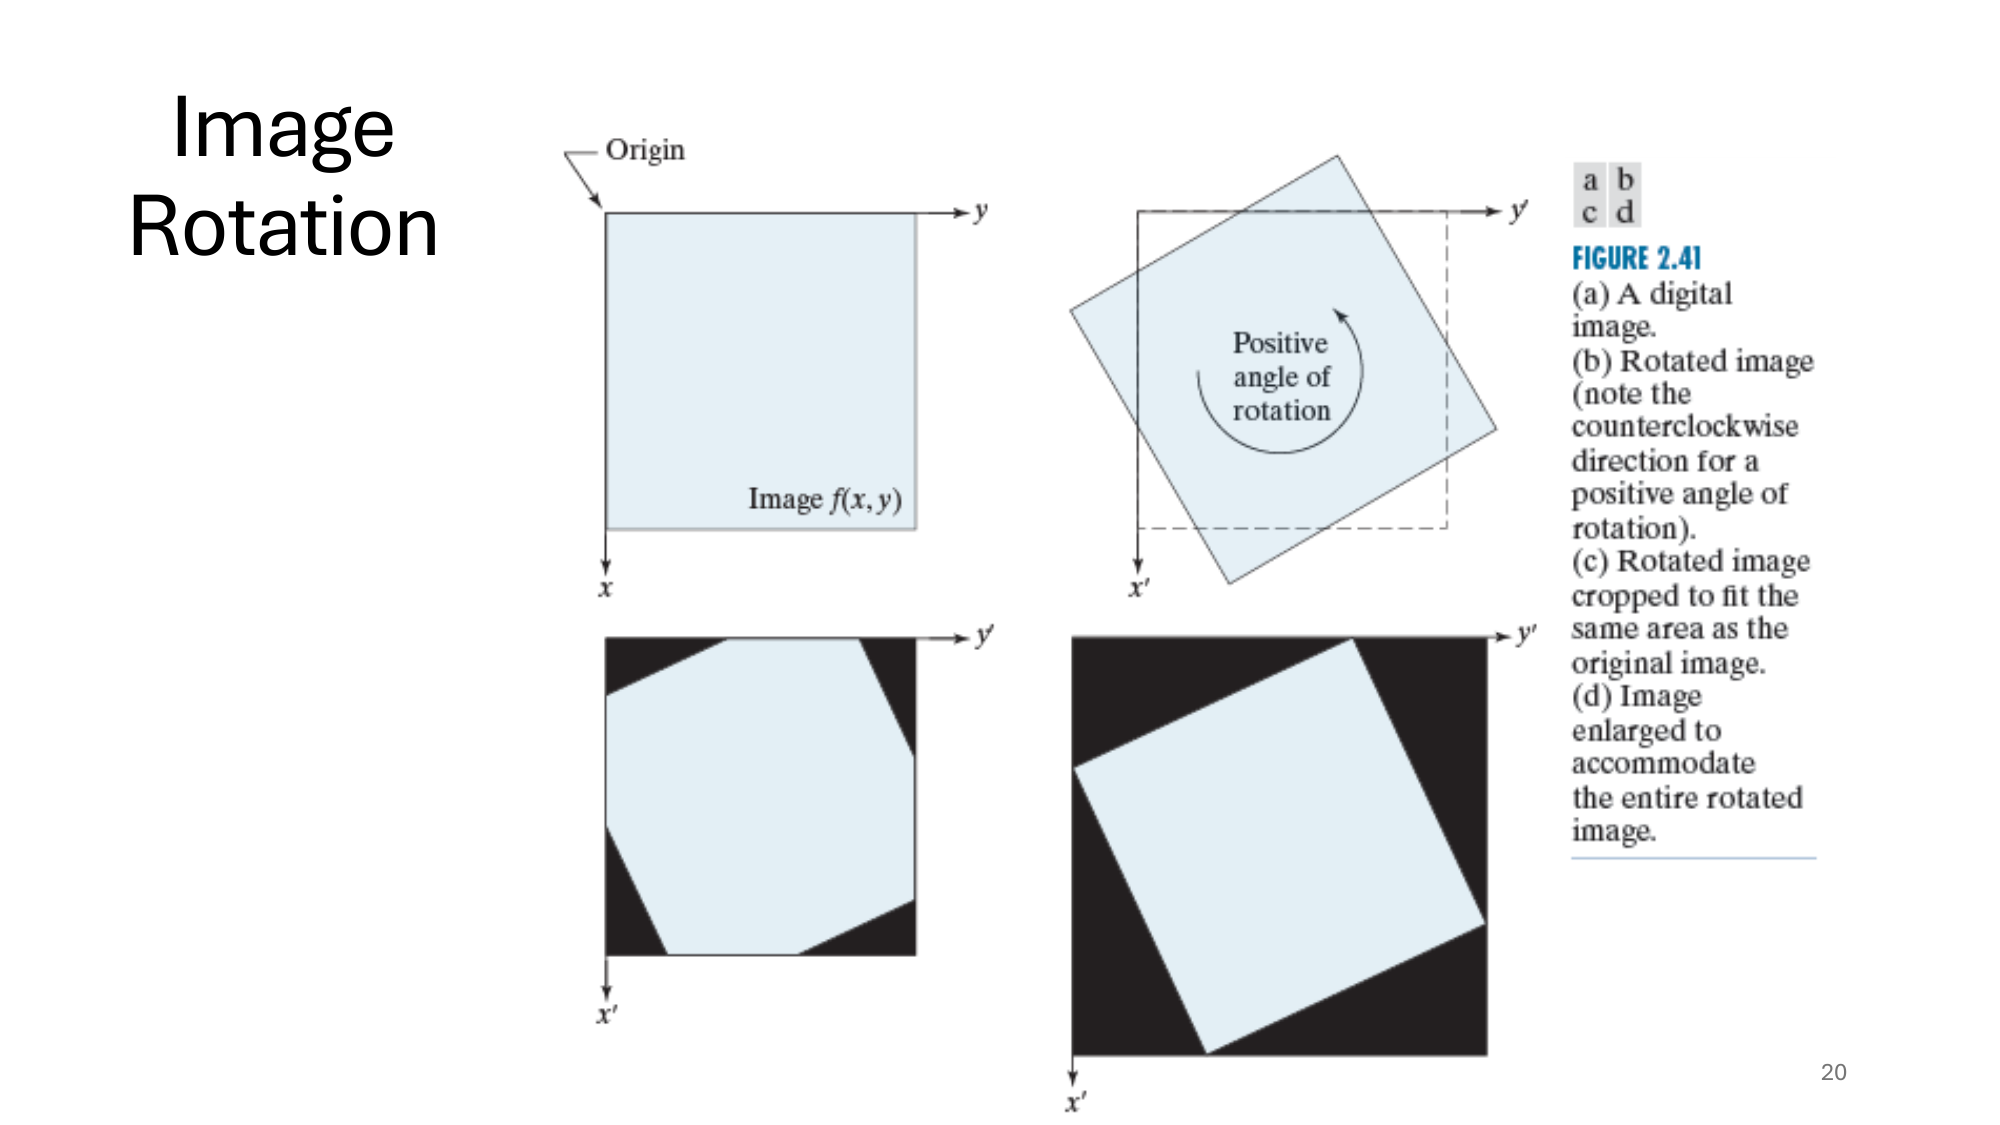
\includegraphics[width=0.85\textwidth]{images/slide4-20.png}
    \caption{Transformation application examples}
    \label{fig:transform_examples}
\end{figure}

%==============================================================================
\section{Introduction to MATLAB for Image Processing}
%==============================================================================

\begin{conceptbox}[MATLAB as the Standard Tool]
MATLAB (and Python with NumPy/OpenCV) are the standard tools for digital image processing:
\begin{itemize}
    \item Images are stored as matrices/arrays
    \item Rich library of built-in functions
    \item Visualization tools
    \item Image Processing Toolbox (MATLAB)
\end{itemize}
\end{conceptbox}

\begin{figure}[H]
    \centering
    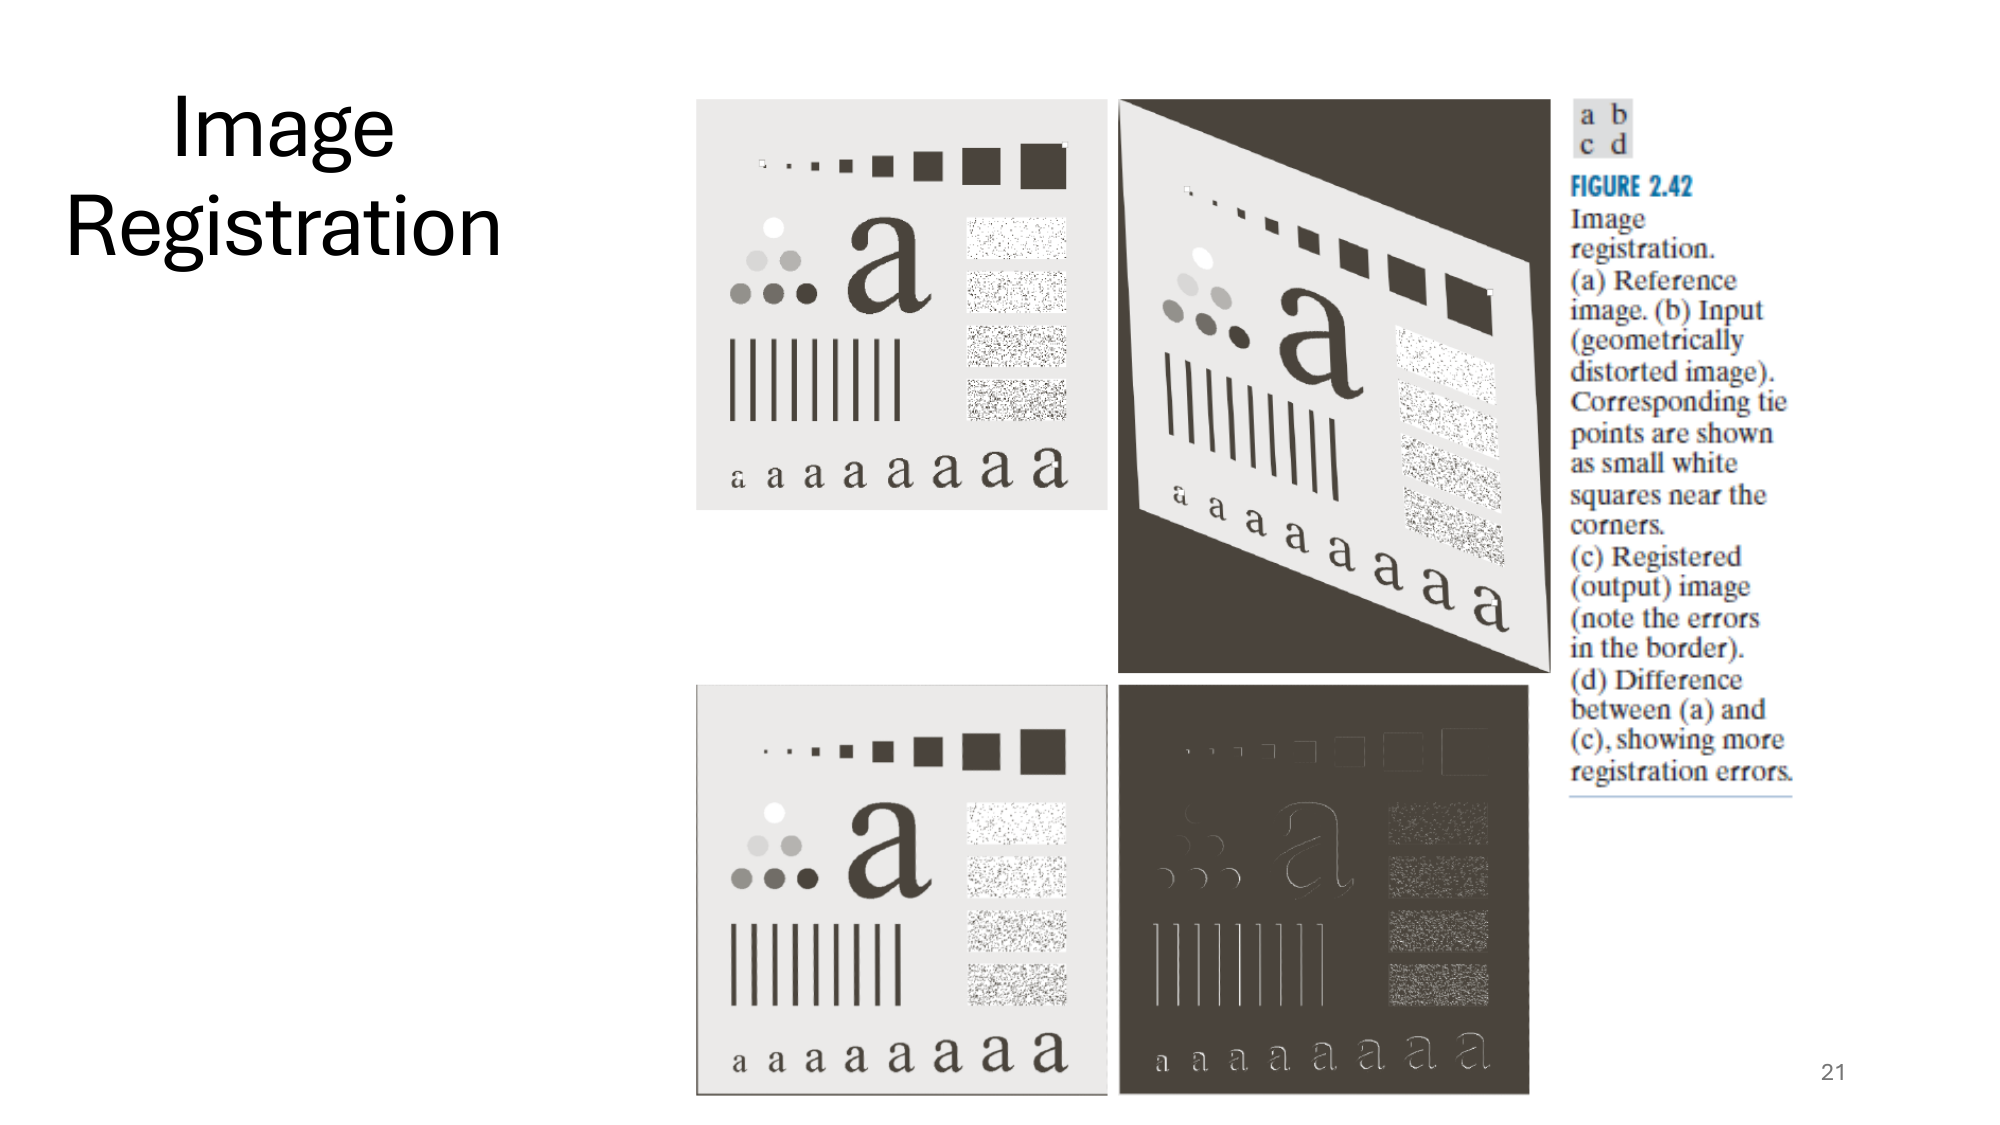
\includegraphics[width=0.85\textwidth]{images/slide4-21.png}
    \caption{Basic image operations in MATLAB}
    \label{fig:matlab_basic}
\end{figure}

\begin{deepexplanation}
\textbf{DEEP ANALYSIS - Figure \ref{fig:matlab_basic}: Programming with Images}

\textbf{Reading and Displaying Images:}
\begin{verbatim}
% Read image from file
img = imread('photo.jpg');

% Display image
imshow(img);

% Get image information
[M, N, channels] = size(img);  % dimensions
class(img)  % data type (uint8, double, etc.)
\end{verbatim}

\textbf{Image Data Types:}
\begin{center}
\begin{tabular}{|l|l|l|}
\hline
\textbf{Type} & \textbf{Range} & \textbf{Use} \\
\hline
uint8 & 0--255 & Most common, 8-bit images \\
uint16 & 0--65535 & 16-bit medical images \\
double & 0.0--1.0 & Computation, processing \\
logical & 0 or 1 & Binary images \\
\hline
\end{tabular}
\end{center}

\textbf{Converting Between Types:}
\begin{verbatim}
img_double = im2double(img);  % uint8 to [0,1]
img_uint8 = im2uint8(img_double);  % back to uint8
\end{verbatim}

\textbf{Accessing Pixels:}
\begin{verbatim}
pixel = img(row, col);  % grayscale
pixel = img(row, col, :);  % color (R,G,B)

% Modify a region
img(100:200, 150:250) = 0;  % set to black
\end{verbatim}
\end{deepexplanation}

\begin{figure}[H]
    \centering
    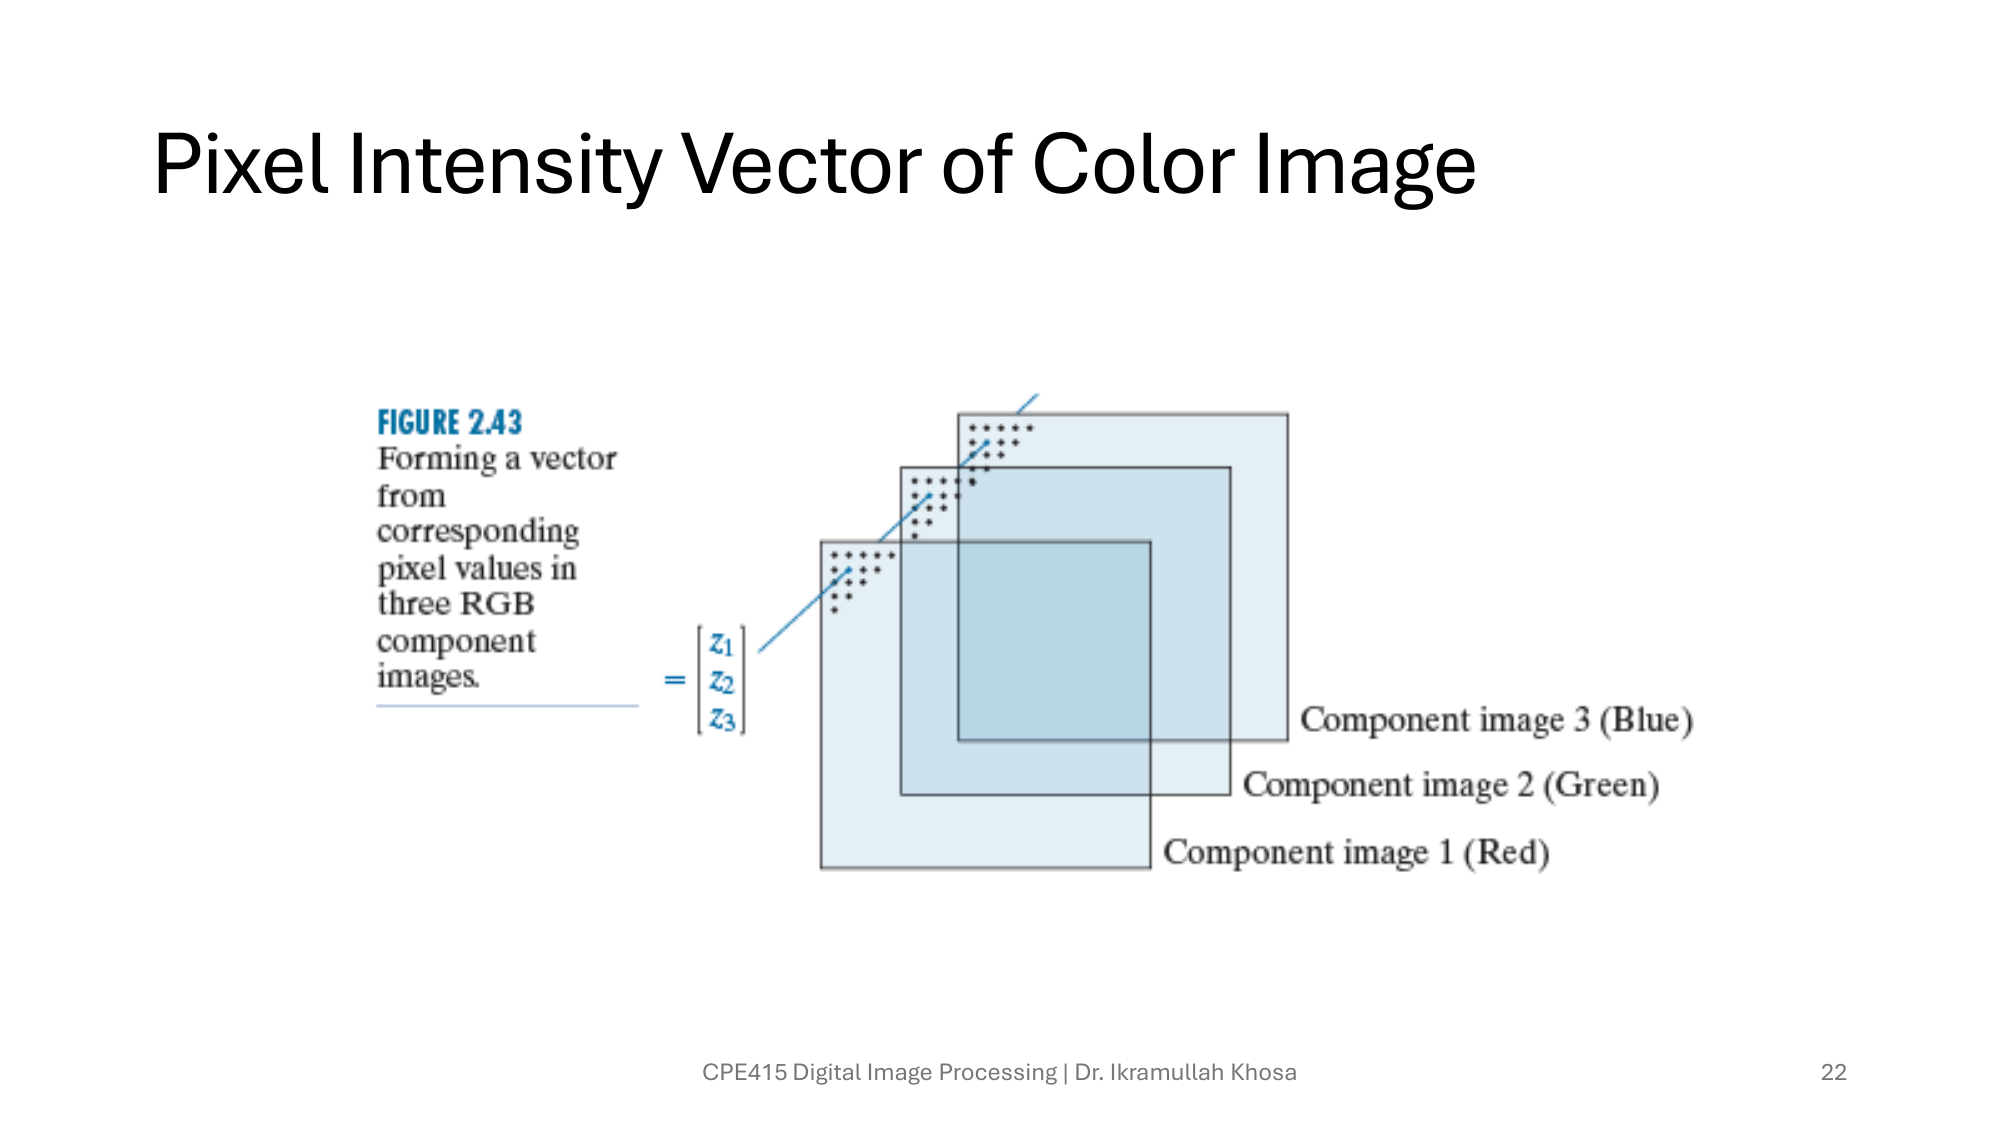
\includegraphics[width=0.85\textwidth]{images/slide4-22.png}
    \caption{Image type conversions}
    \label{fig:matlab_types}
\end{figure}

\begin{figure}[H]
    \centering
    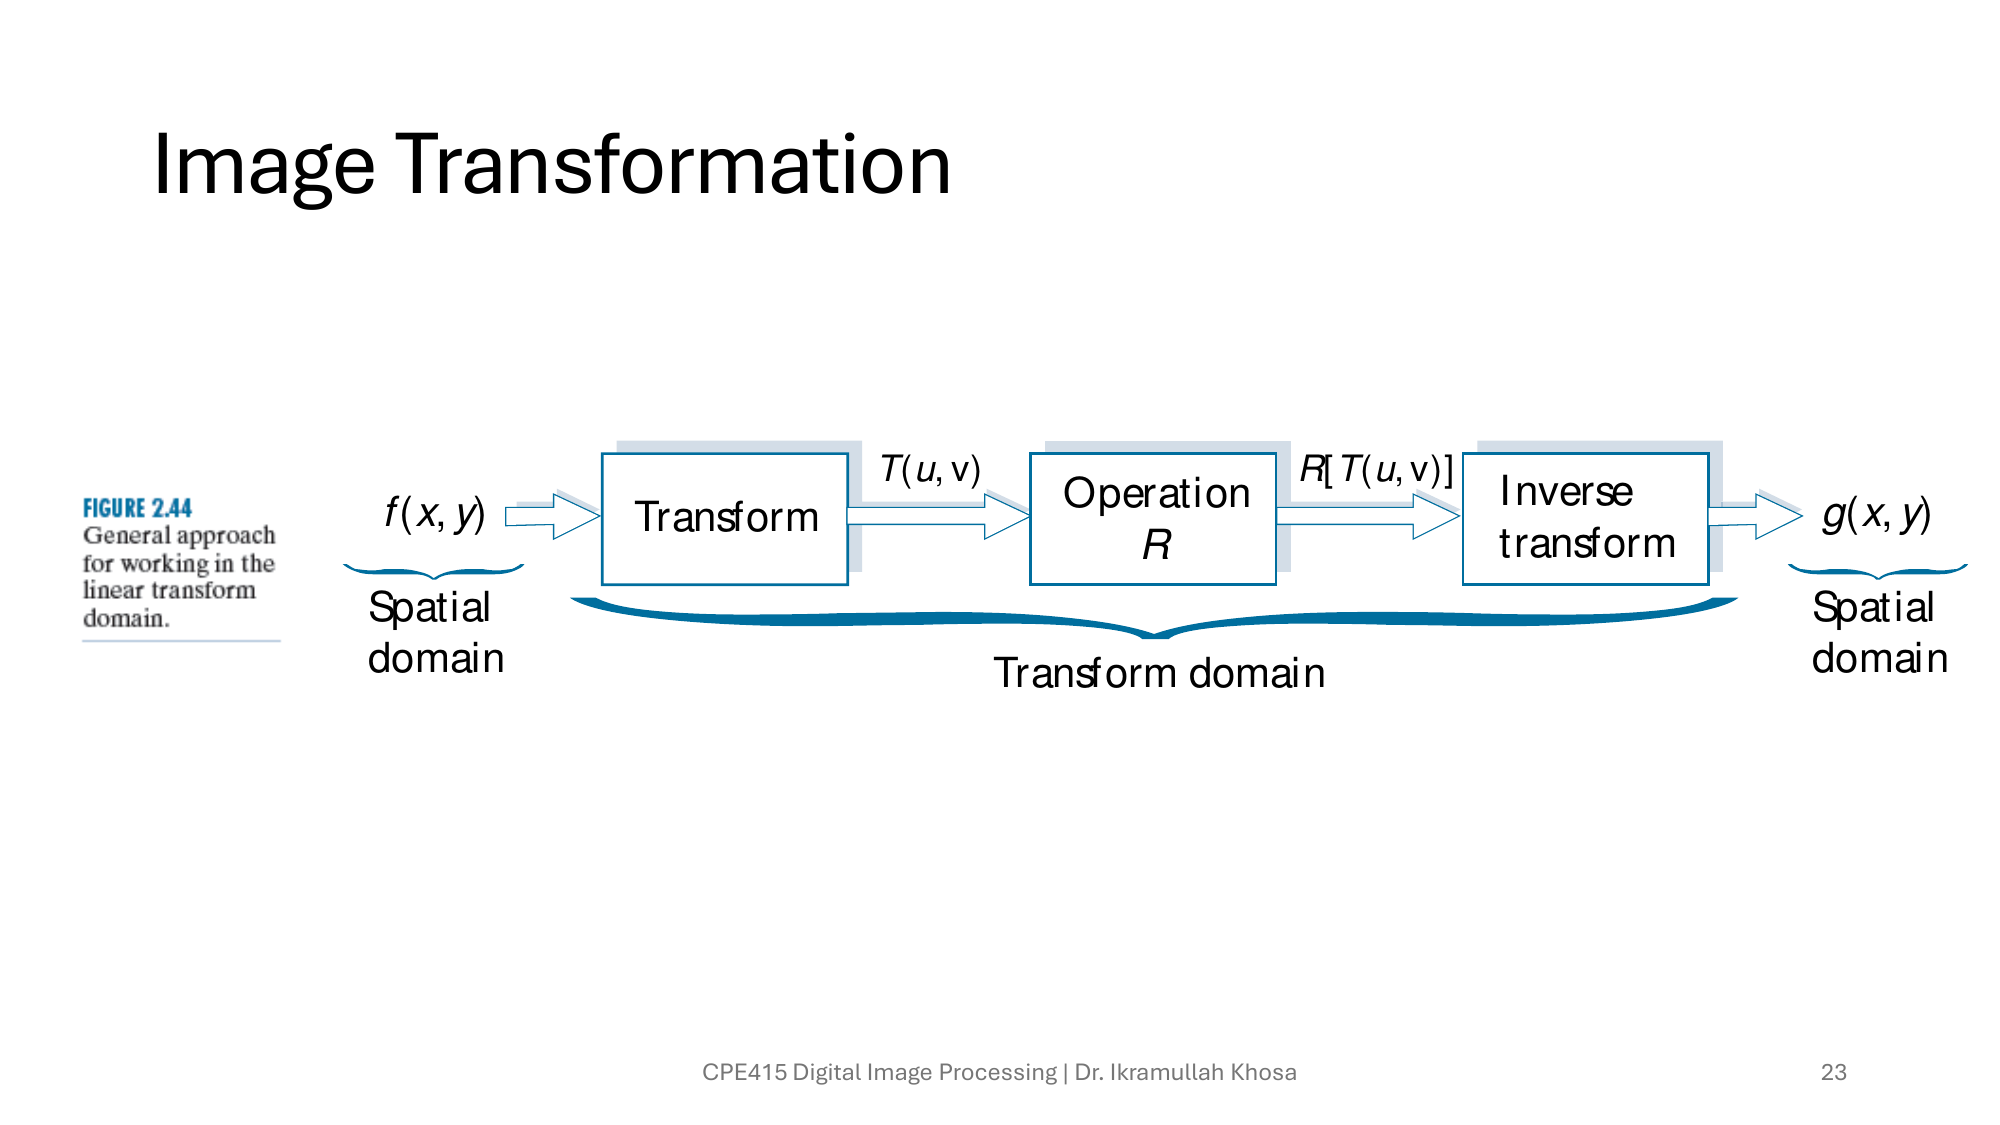
\includegraphics[width=0.85\textwidth]{images/slide4-23.png}
    \caption{Common image processing functions}
    \label{fig:matlab_functions}
\end{figure}

\begin{deepexplanation}
\textbf{DEEP ANALYSIS - Figure \ref{fig:matlab_functions}: Essential Functions}

\textbf{Basic Operations:}
\begin{verbatim}
% Arithmetic
C = A + B;  % addition (watch for overflow!)
C = imsubtract(A, B);  % safe subtraction
C = immultiply(A, B);
C = imdivide(A, B);

% Geometric
B = imresize(A, 0.5);  % shrink by half
B = imresize(A, [256, 256]);  % specific size
B = imrotate(A, 45);  % rotate 45 degrees
B = imcrop(A, [x y width height]);  % crop region
\end{verbatim}

\textbf{Intensity Transformations:}
\begin{verbatim}
% Adjust contrast
B = imadjust(A, [low high], [out_low out_high]);

% Histogram equalization
B = histeq(A);

% Thresholding
B = A > 128;  % binary image
level = graythresh(A);  % Otsu's threshold
B = imbinarize(A, level);
\end{verbatim}

\textbf{Filtering:}
\begin{verbatim}
% Create filter kernel
h = fspecial('gaussian', [5 5], 1);

% Apply filter
B = imfilter(A, h);

% Built-in filters
B = imgaussfilt(A, sigma);  % Gaussian blur
B = medfilt2(A);  % median filter
\end{verbatim}

\textbf{Analysis:}
\begin{verbatim}
% Histogram
[counts, bins] = imhist(A);
imhist(A);  % display histogram

% Statistics
mean2(A)  % mean intensity
std2(A)   % standard deviation
\end{verbatim}
\end{deepexplanation}

\begin{figure}[H]
    \centering
    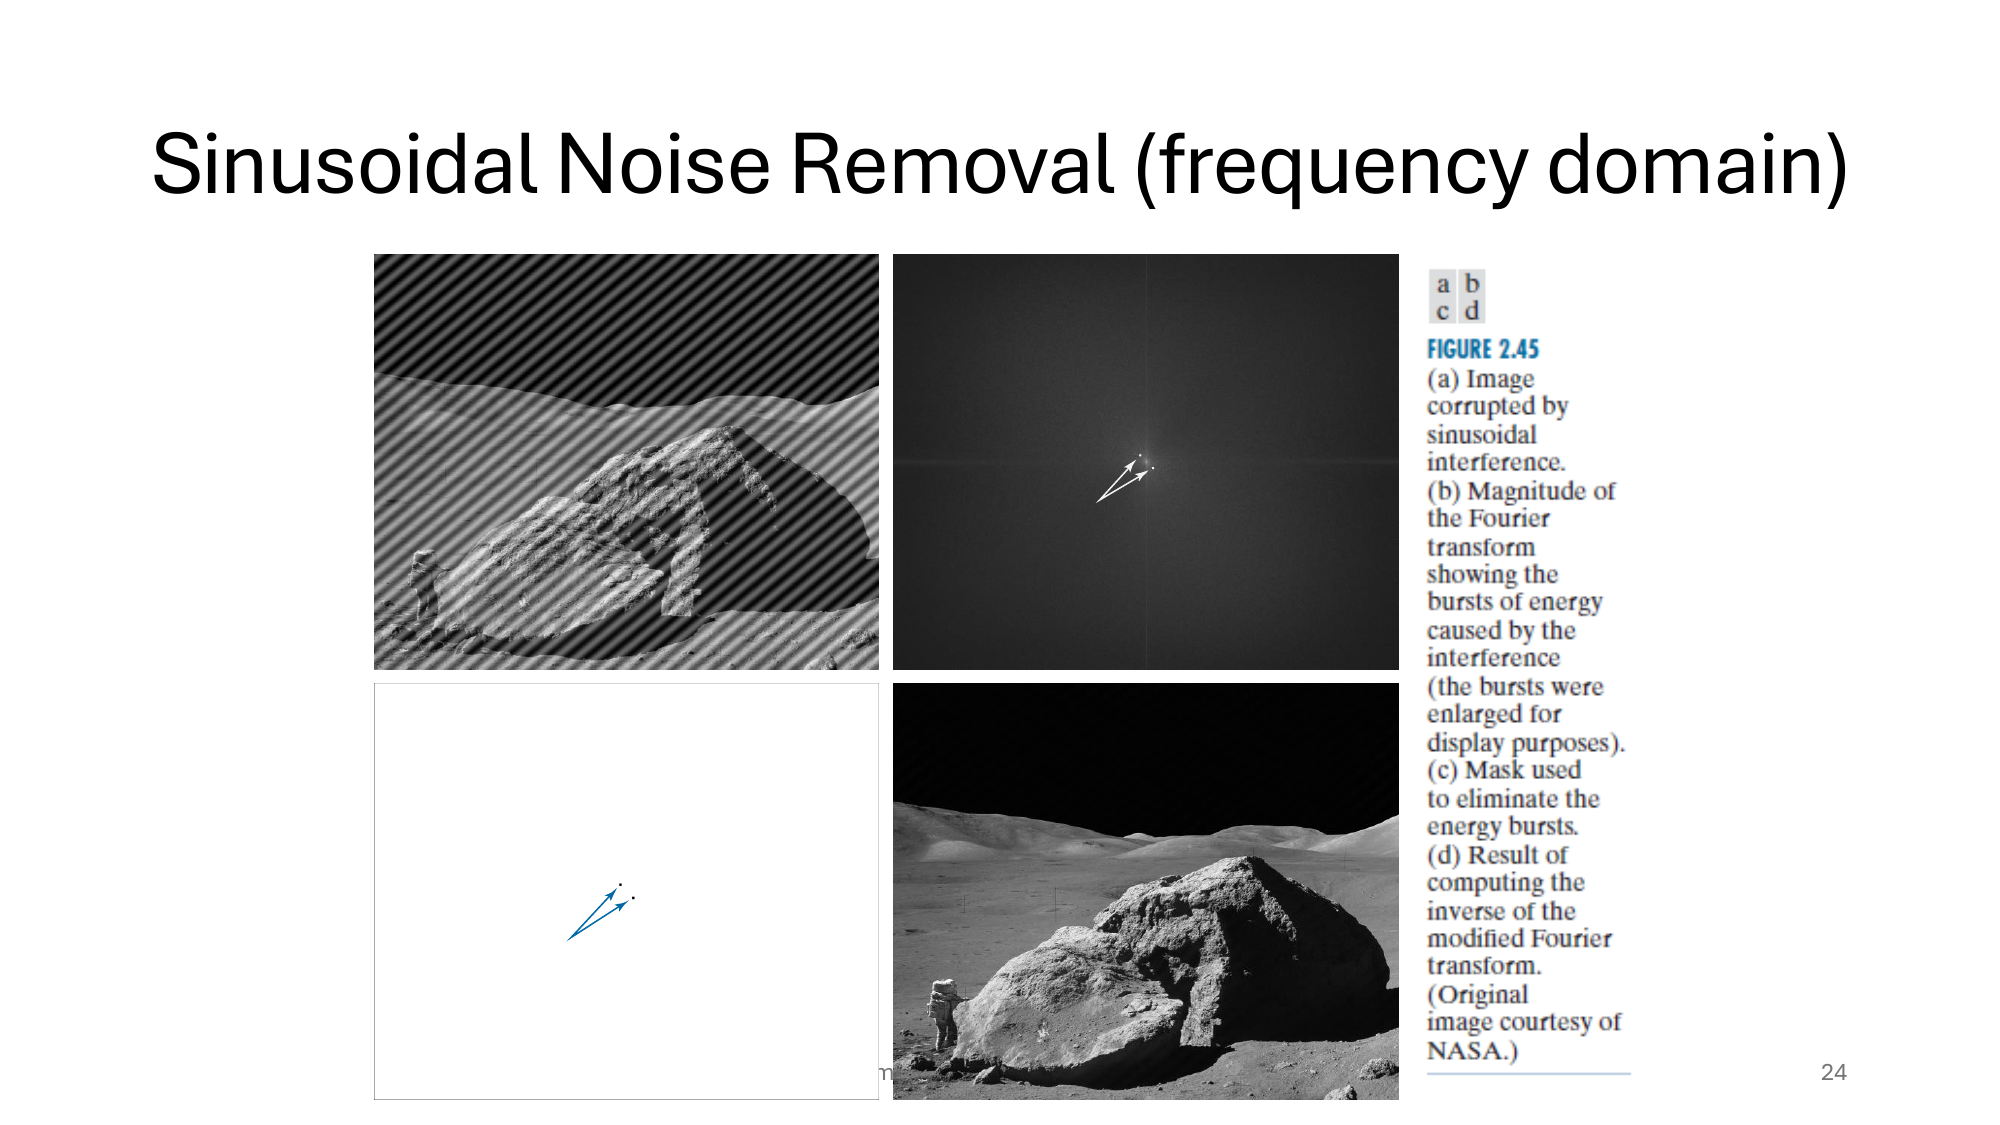
\includegraphics[width=0.85\textwidth]{images/slide4-24.png}
    \caption{Subimage and region operations}
    \label{fig:matlab_regions}
\end{figure}

%==============================================================================
\section{Summary and Key Concepts}
%==============================================================================

\begin{conceptbox}[Chapter 2 Summary]
This chapter covered the fundamental concepts needed to understand digital images:

\textbf{Human Visual System:}
\begin{itemize}
    \item Eye structure: Cornea, lens, retina
    \item Photoreceptors: Cones (color, detail) and Rods (low-light)
    \item Adaptation: Huge dynamic range, but limited simultaneous range
    \item Visual phenomena: Weber's Law, Mach bands, simultaneous contrast
\end{itemize}

\textbf{Image Acquisition:}
\begin{itemize}
    \item Sensor types: Single, linear array, 2D array
    \item Image model: $f(x,y) = i(x,y) \cdot r(x,y)$
\end{itemize}

\textbf{Digitization:}
\begin{itemize}
    \item Sampling: Discretizing spatial coordinates
    \item Nyquist theorem: Sample at $\geq 2 \times$ maximum frequency
    \item Quantization: Discretizing intensity values
    \item Aliasing and false contouring artifacts
\end{itemize}

\textbf{Digital Image Representation:}
\begin{itemize}
    \item Matrix representation: $M \times N$ pixels, $L$ gray levels
    \item Storage: $M \times N \times k$ bits
    \item Dynamic range and contrast
\end{itemize}

\textbf{Resolution:}
\begin{itemize}
    \item Spatial resolution: Pixel density
    \item Intensity resolution: Bits per pixel
    \item Trade-offs captured by isopreference curves
\end{itemize}

\textbf{Interpolation:}
\begin{itemize}
    \item Nearest neighbor: Fast, blocky
    \item Bilinear: Good compromise
    \item Bicubic: Best quality, slowest
\end{itemize}

\textbf{Pixel Relationships:}
\begin{itemize}
    \item Neighborhoods: $N_4$, $N_D$, $N_8$
    \item Adjacency: 4-, 8-, m-adjacency
    \item Connectivity and paths
    \item Distance metrics: $D_E$, $D_4$, $D_8$
\end{itemize}

\textbf{Basic Operations:}
\begin{itemize}
    \item Arithmetic: Addition, subtraction, multiplication, division
    \item Set operations: Union, intersection, complement
    \item Geometric: Translation, rotation, scaling, affine, projective
    \item Image registration
\end{itemize}
\end{conceptbox}

\begin{importantbox}
\textbf{Key Takeaways for Image Processing:}
\begin{enumerate}
    \item Always consider the Nyquist theorem when sampling
    \item Match quantization levels to application needs
    \item Choose interpolation method based on quality/speed trade-off
    \item Use appropriate distance/adjacency definitions for your algorithm
    \item Handle overflow/underflow in arithmetic operations
    \item Use inverse mapping for geometric transformations
\end{enumerate}
\end{importantbox}

%==============================================================================
\section{Practice Problems}
%==============================================================================

\begin{examplebox}[Problem 1: Sampling Calculation]
An analog image has spatial frequency content up to 100 cycles/mm. What is the minimum sampling density (pixels/mm) required to avoid aliasing?

\textbf{Solution:}
By Nyquist theorem: $f_s \geq 2 \times f_{max} = 2 \times 100 = 200$ samples/mm.

So we need at least 200 pixels per mm, or equivalently, a pixel pitch of at most 5 µm.
\end{examplebox}

\begin{examplebox}[Problem 2: Storage Calculation]
Calculate the storage requirement for:
\begin{enumerate}
    \item A $1024 \times 768$ grayscale image with 8 bits/pixel
    \item The same image in 24-bit RGB color
\end{enumerate}

\textbf{Solution:}
\begin{enumerate}
    \item $1024 \times 768 \times 8 = 6,291,456$ bits $= 768$ KB
    \item $1024 \times 768 \times 24 = 18,874,368$ bits $= 2.25$ MB
\end{enumerate}
\end{examplebox}

\begin{examplebox}[Problem 3: Distance Metrics]
Calculate $D_E$, $D_4$, and $D_8$ from pixel $p = (2, 3)$ to pixel $q = (7, 6)$.

\textbf{Solution:}
\begin{itemize}
    \item $D_E = \sqrt{(7-2)^2 + (6-3)^2} = \sqrt{25 + 9} = \sqrt{34} \approx 5.83$
    \item $D_4 = |7-2| + |6-3| = 5 + 3 = 8$
    \item $D_8 = \max(|7-2|, |6-3|) = \max(5, 3) = 5$
\end{itemize}
\end{examplebox}

\end{document}
